\documentclass[
  % Replace twoside with oneside if you are printing your thesis on a single side
  % of the paper, or for viewing on screen.
%  oneside,
  twoside,
  11pt, a4paper, openright
]{book}



\usepackage[left=1in,right=1in,top=1in,bottom=1in]{geometry}
\usepackage{microtype}
\usepackage{cleveref}
\usepackage{xcolor}
\usepackage[draft]{fixme}
\fxusetheme{colorsig}
\FXRegisterAuthor{tgm}{atgm}{TM}
\FXRegisterAuthor{sg}{asg}{SG}
\usepackage{amsmath}
\usepackage{amssymb}
\usepackage{xspace}
\usepackage{complexity}
\usepackage{times}
\usepackage{flafter}
\usepackage{paralist}
\usepackage{enumitem}
\usepackage{amsthm}
\theoremstyle{plain}
% \newtheorem{theorem}{Theorem}
% \newtheorem{lemma}{Lemma}
% \newtheorem{corollary}{Corollary}
% \newtheorem{observation}{Observation}

\theoremstyle{remark}
\newtheorem{remark}{Remark}
\newtheorem{case}{Case}
% \newtheorem{claim}{Claim}[lemma]
% 
% \theoremstyle{definition}
% \newtheorem{definition}{Definition}

\newenvironment{subproof}{%
  \renewcommand{\qedsymbol}{$\Diamond$}%
  \begin{proof}[Proof of Claim]%
}{%
  \end{proof}%
}

\def\DEBUG{true}

\ifdefined\DEBUG
 \newcommand{\tgm}[1]{\textcolor{blue}{#1}}
 \newcommand{\sg}[1]{\textcolor{red}{#1}}
\else
  \newcommand{\tgm}[1]{#1}
  \newcommand{\sg}[1]{#1}
\fi



\usepackage{enumitem}
\setlist{nolistsep, noitemsep, topsep=0pt}

\setcounter{secnumdepth}{2}

\usepackage{tikz}
\usetikzlibrary{calc}
\usetikzlibrary{decorations.markings}
\usetikzlibrary{shapes.geometric,positioning}
\usetikzlibrary{arrows}
\usetikzlibrary{patterns}
\tikzset{node/.style={minimum size=1.8mm,circle,fill=black,draw,inner sep=0pt},
         decoration={markings,mark=at position .5 with {\arrow[black,thick]{stealth}}}}
\tikzset{req/.style={minimum size=1.8mm,circle,fill=white,draw,inner sep=0pt},
         decoration={markings,mark=at position .5 with {\arrow[black,thick]{stealth}}}}

%Environment for restating lemmas
\newcommand{\restated}[2]{
\begin{trivlist}
        \item[\hskip\labelsep {\bf #1} (Restated)] \emph{#2}
\end{trivlist}}

\usepackage[noblocks]{authblk}
\title{A QPTAS for Gapless MEC\footnote{Research partially funded by Deutsche Forschungsgemeinschaft grant MO2889/1-1.}}
\author{Shilpa Garg}
\affil{Max Planck Institute for Informatics, Saarland Informatics Campus, Germany. \texttt{sgarg@mpi-inf.mpg.de}}
\author{Tobias M\"omke}
\affil{Saarland University, Saarland Informatics Campus, Germany. \texttt{moemke@cs.uni-saarland.de}}


\renewcommand{\epsilon}{\varepsilon}
\newcommand{\ie}{i.e.}
\newcommand{\eg}{e.g.}
\newcommand{\WLOG}{w.l.o.g.\xspace}
\newcommand{\cost}{\ensuremath{\mathrm{cost}}\xspace}
\newcommand{\MEC}{\textsc{MEC}\xspace}
\newcommand{\GMEC}{\textsc{Gapless-MEC}\xspace}
\newcommand{\BMEC}{\textsc{Binary-MEC}\xspace}
\newcommand{\SEG}{\textsc{SEG}\xspace}
\newcommand{\GSEG}{\textsc{Gapless-SEG}\xspace}
\newcommand{\dist}{\ensuremath{\mathrm{dist}}\xspace}
\newcommand{\gain}{\ensuremath{\mathrm{gain}}\xspace}
\newcommand{\agree}{\ensuremath{\mathrm{agree}}\xspace}
%\newcommand{\Pr}{\textrm{Pr}}
\newcommand{\euler}{\textrm{e}}
\newcommand{\SWC}{\textsc{SWC}_{\epsilon^3}}

\renewcommand{\DP}[1]{\ensuremath{\mathrm{DP}(#1)}\xspace}
%The following name is used, since \dp already has a meaning in latex.
\newcommand{\CDP}[1]{\ensuremath{\mathrm{dp}(#1)}\xspace}
\newclass{\opt}{opt}
\newclass{\reference}{ref}
\newclass{\UG}{UG}
\usepackage{lipsum}
\usepackage{mathtools}
\usepackage{amsmath}
\usepackage{amsthm}
\usepackage{acronym}
\usepackage{listings}
\usepackage{fancyhdr}
\usepackage[utf8]{inputenc}
\usepackage{color}
\usepackage{balance}
\usepackage{graphicx}
\usepackage{array}
\usepackage{tikz}
\usetikzlibrary{arrows,calc,matrix,shapes,trees,positioning}
\usepackage[boxed,vlined,linesnumbered]{algorithm2e}
\usepackage{booktabs}
\usepackage{tabularx}
\usepackage{rotating}
\usepackage{paralist}
\usepackage{subfigure}
\usepackage{datetime}
\usepackage{multirow}
\usepackage{tipa}
\usepackage{pgfplots}
\usepackage{pgfplotstable}
\usepackage{soul}
\usepackage[T1]{fontenc}
\usepackage{lmodern}
\usepackage{url}
\usepackage[font={bf}]{caption}
\usepackage{amsmath}
\usepackage{amssymb}
\usepackage{listings}
\lstset{language=Java}
\usepackage{moreverb}
%\renewcommand*\ttdefault{lmvtt}
\SetKwComment{Comment}{$\triangleright$\ }{}
\usepackage[english]{babel}
\usepackage{setspace}
\usepackage[bookmarks]{hyperref}
\usepackage{xcolor}
\usepackage{mathtools}
%\usepackage{natbib}
\usepackage{enumitem}
\usepackage{pdflscape}
\usepackage{appendix}
% \usepackage[object=vectorian]{pgfornament}

\setlist[itemize]{leftmargin=*}
\DeclareMathOperator*{\argmin}{arg\,min}


%%Algorithm style
\SetAlFnt{\sffamily}
\setlength{\algoheightrule}{0.8pt} % thickness of the rules above and below
\setlength{\algotitleheightrule}{0.8pt} % thicknes of the rule below the title
%%


\usepackage{titlesec}
\titleformat{\chapter}[display]
{\normalfont\bfseries}
{{\LARGE {\it Chapter}~~}{\HUGE \thechapter}}
{1ex}
{\vspace{2ex}  \huge }
[\vspace{1ex}]

\usepackage{etoolbox}

\makeatletter
\patchcmd{\ttlh@hang}{\parindent\z@}{\parindent\z@\leavevmode}{}{}
\patchcmd{\ttlh@hang}{\noindent}{}{}{}
\makeatother

\hypersetup{
    colorlinks,
    linkcolor={red!50!black},
    citecolor={red!50!black},
    urlcolor={blue!80!black}
}

%\usepackage{unicode-math}
\usepackage{libertine}
\usepackage[italic]{mathastext}
\renewcommand{\ttdefault}{cmtt}
%\renewcommand{\sfdefault}{lmss}
%\usepackage{euler}


\usepackage{bbm}
\usepackage{amsthm}
\usepackage{amssymb}
\usepackage{stmaryrd}
\usepackage{url}



\newcommand{\todo}[1]{\textbf{[TODO: #1]}}
\newcommand{\N}{\mathbbm{N}}
\newcommand{\cupdot}{\dot{\cup}}
\newcommand{\iverl}{\llbracket}
\newcommand{\iverr}{\rrbracket}
\newcommand{\abs}[1]{{\left\lvert #1 \right\rvert}}
\usepackage{amsfonts}

%\setmathfont{Latin Modern Math}
%\setmathfont[range=\mathit/{latin,Latin,num,Greek,greek}]{Linux Biolinum O Italic}
%\setmathfont[range=\mathup/{latin,Latin,num,Greek,greek}]{Linux Biolinum O}
%\setmathfont[range=\mathbfup/{latin,Latin,num,Greek,greek}]{Linux Biolinum O Bold}
%\setmathfont[range={\mathrm,0048-0057}]{Linux Biolinum O}

 \newtheorem{theorem}{\normalfont{\scshape Theorem}}[chapter]
 \newtheorem{lemma}{\normalfont{\scshape Lemma}}[chapter]
 \newtheorem{claim}{\normalfont{\scshape Claim}}[chapter]
 \newtheorem{proposition}{\normalfont{\scshape Proposition}}[chapter]
 \newtheorem{corollary}{\normalfont{\scshape Corollary}}[chapter]
 \newtheorem{observation}{\normalfont{\scshape Observation}}[chapter]
 \newtheorem{definition}{\normalfont{\scshape  Definition}}[chapter]
 \newtheorem{example}{\normalfont{\scshape Example}}[chapter]
 \newtheorem{problem}{\normalfont{\scshape Problem}}[chapter]
 \newtheorem{weakness}{\normalfont{\scshape Weakness}}[chapter]
  \newtheorem{gaps}{\normalfont{\scshape Open Problem}}[chapter]
 
 

 \newcommand{\squishlist}{
 \begin{list}{$\bullet$}
  { \setlength{\itemsep}{0pt}
     \setlength{\parsep}{1pt}
     \setlength{\topsep}{1pt}
     \setlength{\partopsep}{0pt}
     \setlength{\leftmargin}{3em}
     \setlength{\labelwidth}{1em}
     \setlength{\labelsep}{0.5em} } }
 \newcommand{\squishend}{\end{list}}

 %%%% Tikz related libraries
\usetikzlibrary{positioning,shapes,shadows,arrows}
\usetikzlibrary{patterns}
\usepgfplotslibrary{groupplots}
\usetikzlibrary{trees}
\setlength{\textfloatsep}{5pt}
\setlength{\floatsep}{0pt}
\setlength{\intextsep}{0pt}
%%%%

%%%% Misc
%\newcommand{\verbatimfont}[1]{\def\verbatim@font{#1}}%
%\verbatimfont{\sffamily}

\def\CC{{C\nolinebreak[4]\hspace{-.05em}\raisebox{.4ex}{\tiny\bf ++}}}
\def\Giraphpp{{Giraph\nolinebreak[4]\hspace{-.05em}\raisebox{.4ex}{\tiny\bf ++}}}
\def\vgap{\vspace*{0.3cm}}
\def\sf{\sffamily}
%%%%


%%% bib
% \usepackage[backref=true]{biblatex}
% \usepackage{hyperref}
% \DefineBibliographyStrings{english}{%
%   backrefpage = {page},% originally "cited on page"
%   backrefpages = {pages},% originally "cited on pages"
% }

 \usepackage{natbib}%
% \hypersetup{urlcolor=blue, colorlinks=true}
% \usepackage{backref}

%%% 


\setlength{\headheight}{15.2pt}

%%% Header conf
\fancypagestyle{fancybook}{%
    \fancyhf{}%
    % Note the ## here. It's required because \fancypagestyle is making a macro (\ps@fancybook).
    % If we just wrote #1, TeX would think that it's the argument to \ps@fancybook, but
    % \ps@fancybook doesn't take any arguments, so TeX would complain with an error message.
    % You are not expected to understand this.
    \renewcommand*{\sectionmark}[1]{ \markright{\thesection\ ##1} }%
    \renewcommand*{\chaptermark}[1]{ \markboth{\chaptername\ \thechapter: ##1}{} }%
    % Increase the length of the header such that the folios
    % (typography jargon for page numbers) move into the margin
    \fancyhfoffset[LE]{6mm}% slightly less than 0.25in
    \fancyhfoffset[RO]{6mm}%
    % Put some space and a vertical bar between the folio and the rest of the header
    \fancyhead[LE]{\nouppercase{\sf \thepage~|~~{\slshape \leftmark}}}%
    %\fancyhead[LE]{\thepage\hfill{\leftmark}}%
    \fancyhead[RO]{\nouppercase{\sf {\slshape \rightmark}~~|~\thepage}}%
%    \fancyfoot[C]{{\thepage}}
}

%% (more) Tikz definitions
% Graphs
\tikzstyle{boundary}=[circle,fill=black!25,minimum size=15pt,inner sep=0pt]
\tikzstyle{vertex}=[circle,draw,minimum size=15pt,inner sep=0pt]

%% tikz
 \tikzset{
    line/.style = {draw},
    block/.style = {rounded rectangle,fill, text centered, minimum height=0.4em, inner sep=1pt},
    greyblock/.style = {fill=black!10, rounded rectangle,draw, text centered, minimum height=1em},
}
%%


% Query
\definecolor{query-color}{RGB}{240,240,235}
\tikzstyle{query}=[draw=query-color,fill=query-color,inner sep=6pt]

%Queries

\newcommand{\sparqlq}{

}



%%% Local Variables:
%%% mode: latex
%%% TeX-master: "main"
%%% End:

%%


\usepackage{afterpage}

\newcommand\blankpage{%
    \null
    \thispagestyle{empty}%
%    \addtocounter{page}{-1}%
    \newpage}

\begin{document}



%\pagenumbering{gobble}
\pagenumbering{roman}

\pagestyle{empty}
{

\centering

\vspace*{2cm}

{
\setstretch{1.5}

% \begin{center}
% \pgfornament[width=2cm,symmetry=h]{88}
% %\pgfornament[width=5cm,symmetry=h]{49}
% %\pgfornament[width=10cm]{49}
% \end{center}


{\LARGE \textbf{Computational Haplotyping: theory and practice }}%of Large Labelled Graphs}}





\vspace*{2cm}
{\large \textbf {Shilpa Garg}}

%\text{Max-Planck Institute for Informatics}

}

\vspace*{4cm}


\text{Thesis for obtaining the title of Doctor of Engineering}

\text{of the Faculty of Mathematics and Computer Science}

\text{of Saarland University}

%\vfill
\vspace*{4cm}

{ \large Saarbr\"ucken \\ 2018}

\vfill
}


%%% Local Variables:
%%% mode: latex
%%% TeX-master: "../main"
%%% End:

%\pagestyle{plain}
{

\vspace*{2cm}
{

{\bf Colloquium}
\vspace*{5mm}

\begin{tabular}{lrl}
Date &\hspace*{3.9cm:}&\\
Place &:&\\
Dean &:&
\end{tabular}

\vspace*{1cm}

{\bf Examination Board}

\vspace*{5mm}
\begin{tabular}{lrl}
Chairman&\hspace*{2cm:}&\\
Reviewer &:&\\
Reviewer &:&\\
Reviewer &:&\\
Scentific Assitant &:&
\end{tabular}


}

%%% Local Variables:
%%% mode: latex
%%% TeX-master: "../main"
%%% End:

\pagestyle{fancybook}
%*******************************************************
% Abstract
%*******************************************************
%\pdfbookmark[1]{Abstract}{Abstract}
\chapter*{Abstract}

Genomics has paved a new way to comprehend life and its evolution, and also to investigate causes of diseases and their treatment.
One of the important problems in genomic analyses is haplotype assembly. Constructing complete and accurate haplotypes plays an essential role in understanding population genetics and how species evolve.
In this thesis, we focus on computational approaches to haplotype assembly from third generation sequencing technologies.
This involves huge amounts of sequencing data, and such data contain errors due to the single molecule sequencing protocols employed. 
Taking advantage of combinatorial formulations helps to correct for these errors to solve the haplotyping problem.
Various computational techniques such as dynamic programming, parameterized algorithms, and graph algorithms are used to solve this problem.

This thesis presents several contributions concerning the area of haplotyping. First, a novel algorithm based on dynamic programming is proposed to provide approximation guarantees for phasing a single individual.
Second, an integrative approach is introduced to combining multiple sequencing datasets to generating complete and accurate haplotypes.
The effectiveness of this integrative approach is demonstrated on a real human genome.
Third, we provide a novel efficient approach to phasing pedigrees and demonstrate its advantages in comparison to phasing a single individual.
Fourth, we present a generalized graph-based framework for performing haplotype-aware de novo assembly. 
Specifically, this generalized approach consists of a hybrid pipeline for generating accurate and complete haplotypes from data stemming from multiple sequencing technologies, one that provides accurate reads and other
that provides long reads.

% In summary, this thesis introduces novel computational approaches to generating haplotypes, which make a significant contribution to
% the field of genetics, further opening up avenues for developing life saving technologies.

\chapter*{Kurzfassung}

Die Genomik hat neue Wege eröffnet, die es ermöglichen, die Evolution lebendiger Organismen zu verstehen, sowie die Ursachen zahlreicher Krankheiten zu erforschen und neue Therapien zu entwickeln.
Ein wichtiges Problem ist die Assemblierung der Haplotypen eines Individuums. Diese Rekonstruktion von Haplotypen spielt eine zentrale Rolle für das Verständnis der Populationsgenetik und der Evolution einer Spezies.
In der vorliegenden Arbeit werden Algorithmen zur Assemblierung von Haplotypen vorgestellt, die auf Sequenzierdaten der dritten Generation basieren. Dies erfordert große Mengen an Daten, welche wiederum Fehler enthalten,
die die zugrunde liegenden Sequenzierprotokolle hervorbringen. Durch kombinatorische Formulierungen des Problems ist die Rekonstruktion von Haplotypen dennoch möglich, da Fehler erfolgreich korrigiert werden können.
Verschiedene informatische Methoden, wie dynamische Programmierung, parametrisierte Algorithmen und Graph Algorithmen können verwendet werden, um dieses Problem zu lösen.

Die vorliegende Arbeit stellt mehrere Lösungsansätze für die Rekonstruktion von Haplotypen vor.
Als erstes wird ein neuartiger Algorithmus vorgestellt, der basierend auf dem Prinzip der dynamischen Programmierung Approximationsgarantien für das Haplotyping eines einzelnen Individuums
liefert.
Als zweites wird ein integrativer Ansatz präsentiert, um mehrere Sequenzierdatensätze zu kombinieren und somit akkurate Haplotypen zu generieren.
Die Effektivität dieser Methode wird auf einem echten, menschlichen Datensatz demonstriert.
Als drittes wird ein neuer, effizienter Algorithmus beschrieben, um Haplotypen verwandter Individuen simultan zu konstruieren und die Vorteile gegenüber der Betrachtung einzelner Individuen aufgezeigt.
Als viertes präsentieren wir eine Graph-basierte Methode um mittels Haplotypinformation de-novo Assemblierung durchzuführen. Dieser Algorithmus kombiniert Daten stammend von verschiedenen Sequenziertechnologien, welche entweder
genaue oder aber lange Sequenzierreads liefern.


 

%%% Local Variables:
%%% mode: latex
%%% TeX-master: "../main"
%%% End:

%%*******************************************************
% Dedication
%*******************************************************
\thispagestyle{empty}
%\pdfbookmark[1]{Dedication}{Dedication}

\vspace*{3cm}

\begin{center}
    To my mother
\end{center}

%*******************************************************
% Acknowledgments
%*******************************************************
%\pdfbookmark[1]{Acknowledgements}{acknowledgements}
\chapter*{Acknowledgements}

I would like to express my deep gratitude to all the people who supported me during this work.

First and foremost, I am grateful to my supervisor Dr Tobias Marschall who introduced me to this haplotyping problem, 
helped me to develop problem solving skills for solving a research problem,
and provided me his able guidance in completing this thesis work. 
I would like to offer special thanks to Prof Thomas Lengauer for providing me his valuable remarks on an earlier version of some of the chapters of this thesis and the financial support.
Thanks a million to Prof George Church for his consent to give time to review this thesis.

I am deeply grateful to Prof Richard Durbin whose lab I visited for my research internship.
His enthusiasm for genomics and guidance on future career prospects largely motivated me.
Dr Tobias Mömke has been great source of inspiration and advice for me.
His problem solving ability has been a source of encouragement for me.

I am immensely thankful to all collaborators and coauthors for their support and assistance.
It was great working with David Porubsky and Ashley Sanders, and learning the magic of Strand-Seq technology.
Thanks to Mikko Rautiainen and vgteam for great discussions on the graph world of genomics.

I appreciate the discussions with my office-mate Ali Ghaffaari on violin and classical music.
Special thanks to Jana for always providing a friendly support and guidance.
I would like to extend my thanks to my group mates, who organized different events at weekends. The events were enjoyable experiences.

Jana, Fabio, Lara, Prabhav and Adam proofread a few chapters of this thesis and I greatly appreciate their valuable remarks and feedback.

I appreciate the travel financial support from Michelle Carnell, technical help from Achim, George and MPII-IST and other administrative help from Susanne and Ruth.  

Finally, I would like to express the gratitude to my family and friends, who greatly helped me in this journey.





%%% Local Variables:
%%% mode: latex
%%% TeX-master: "../main"
%%% End:

%%*******************************************************
% Declaration
%*******************************************************
%\pdfbookmark[0]{Declaration}{declaration}
\chapter*{Declaration}
\thispagestyle{empty}

Put your declaration here.


%*******************************************************
% Table of Contents
%*******************************************************
%\pdfbookmark[1]{\contentsname}{tableofcontents}

\setcounter{tocdepth}{2} % <-- 2 includes up to subsections in the ToC
\setcounter{secnumdepth}{3} % <-- 3 numbers up to subsubsections

\tableofcontents 

% %*******************************************************
% % List of Figures and of the Tables
% %*******************************************************

% %*******************************************************
% % List of Figures
% %*******************************************************    
% %\pdfbookmark[1]{\listfigurename}{lof}
% \listoffigures

% %*******************************************************
% % List of Tables
% %*******************************************************
% %\pdfbookmark[1]{\listtablename}{lot}
% \listoftables
  
% %*******************************************************
% % List of Listings
% %******************************************************* 
% %\pdfbookmark[1]{\lstlistlistingname}{lol}
% \lstlistoflistings 
   
% %*******************************************************
% % Acronyms
% %*******************************************************
% %\pdfbookmark[1]{Acronyms}{acronyms}
% \chapter*{Acronyms}
% \begin{acronym}[UML]
%     \acro{DRY}{Don't Repeat Yourself}
%     \acro{API}{Application Programming Interface}
%     \acro{UML}{Unified Modeling Language}
% \end{acronym} 

%%% Local Variables: 
%%% mode: latex
%%% TeX-master: "../main"
%%% End: 




\pagenumbering{arabic}
\setcounter{page}{0}
\chapter{Introduction}

% In this chapter, we introduce the fundamentals of genetics and DNA sequencing. Furthermore, we introduce the important research problem in the field of genetics, the diploid genome assembly (haplotyping). 
% We will see how we can mathematically formualate the diploid assembly problem as a computer scientist.
% Then we provide a high level description of the main methods used in this problem.
% Thereafter, we describe the limits and challenges faced currently in this field. We finish this chapter by an outline of the thesis.


Genetics studies the phenomenon of \textit{life} at its most basic level, thus the science of genetics is important and fascinating.
% In this section we describe the basics about genetics and haplotyping. We provide motivation about why understanding genetics for different organisms is so important.
% https://www.gen.cam.ac.uk/undergraduate/whygenetics
% http://www.helsinki.fi/biosciences/genetics/
An important field in genetics is haplotyping.
Haplotyping is the process of determining the sequences of both copies of homologous chromosomes, which are inherited from each parent in diploid organisms.
Haplotyping has applications in different fields such as evolutionary studies, clinical diagnosis, precision medicine, and biotechnology. 
Current sequencing technologies allow for reading off the genome sequence, and thus the reconstruction of haplotypes is
possible, in principle. Unfortunately, sequencing is prone to errors and the use of advanced algorithms and models is essential to correct for errors, in order to reconstruct accurate haplotypes.
However, the process of correcting these errors poses various computational challenges.
In this thesis, we present our novel algorithms to addressing various computational challenges in this field.

\section{Genetics, DNA sequencing and Haplotyping}\label{sec:dna_seq}
Genetics is the study of genes, genetic variation, and heredity in living organisms. 
Genetics controls what an organism looks like and how it functions.
% The DNA is the carrier of hereditary information and thus understanding DNA in detail has been the central aim for many researchers.
% Classically the genetic variants (mutations) present in the living organisms have been used to study and investigate the cause of biological diseases and, additionally helps to make deductions about the way cells and organisms worked. 
% Genetics is the study of genes, genetic variation, and heredity in living organisms.
Specifically, there are two sides to the science of genetics.
On the one hand, the availability of different types of molecular information, such as sequence information and gene expression levels, paired with gene editing techniques with which we can perturb the genome in a controlled fashion and observe its biological effects, 
provides powerful explanation about the functions of the genes.
On the other hand, genetics provides a fundamental understanding of how organisms, populations, and species evolve. 
In the last few years, one of the most exciting new developments is the way in which these two sides have begun to converge \citep{casillas2017molecular}.
This convergence is achieved through the development of sequencing technologies that provide datasets from the genomic level to epigenomic, transcriptomic, proteomics or metabolomic level.
% The integrative analyses of these datasets promise to provide a systematic view of the causes and consequences of evolution, development and functions of organisms.

% these vary during the lifetime of the individual, therefore, have the potential to provide insights  effort of using molecular techniques to understand the processes of development, evolution, and speciation.
% % Modern computational biology tools (analysis of genomic sequences and bioinformatics) use these integrative principles 
% % to answer various difficult biological questions ranging from the mechanisms of evolution to the development of complex diseases.
% Thus, genetics has a central role in modern biology and its influence is ever increasing.

% s\todo{citations are missing in this para or even figures.}
% from italy person thesis.
\textit{What actually is genetic information?} 
The discovery of spatial structure of double helix deoxyribonucleic acid (DNA) by Watson and Crick in 1953, laid the main foundation for the understanding of genetics.
In most living organisms, genetic information is encoded in the form of DNA molecules.
A DNA molecule is a chain in which many bases are ordered in a linear sequence, the bases --- A, T, G, and C --- are the letters of the genetic alphabet.
The whole information within the DNA molecule of an organism is called its genome. The genome is further divided into chromosomes.
Genomes have single (haploid), double (diploid) or higher ploidy with more than two homologous chromosomes (polyploids). 
In this study, we focus on \textit{diploid} organisms. For example, humans are diploids, consisting of two copies of each chromosome called homologous chromosomes or \textit{haplotypes} --- one inherited from the mother and the other from the father.
There are differences between these two copies of each chromosome known as genetic variation. 
% \todo{this para explained in more detail in biological background.}

In early 2000s, a historic breakthrough happened with the sequencing of the human genome \citep{collins2003human}.
\textit{Sequencing} is the operation that comprises in determining the base sequence of a DNA molecule.
For sequencing genomes, there exist several kinds of sequencing technologies which share the following common properties:
\begin{itemize}
 \item They yield genomes in fragments called ``reads''.
 \item The position of reads along the genome sequence is unknown and also, mostly, the strand from which the read was sampled is unknown.
 \item The reads contain errors.
\end{itemize}

\bigskip
Huge amounts of sequencing data are produced by next generation sequencing technologies (NGS) routinely. 
The major challenge with these sequencing datasets is that the genomic information is partial and erroneous. Therefore, no sequencing technology delivers data from which we can assemble the complete genome.

The sequencing technologies differ in terms of error rates and lengths of the produced reads. We define the error rate of a read as the ratio of the number of incorrectly sequenced bases to the length of the read.
Broadly, the sequencing technologies can be categorized into four classes:
\begin{itemize}
 \item Short read sequencing: It includes Illumina/Solexa sequencing \citep{bentley2008accurate}, which has been the most widespread technology. 
 This technology produces short reads (hundreds of bases) with an error rate ($\le 1$\%). 
  \item Long read sequencing: This approach includes Single Molecule Real Time sequencing (PacBio) \citep{eid2009real} and Oxford Nanopore sequencing (ONT) \citep{laszlo2014decoding}. These technologies produce very long sequences, up to hundreds of kilo-bases. 
  The downside is that PacBio and ONT exhibit very high error rates of up to 15\% and 38\% respectively. 
  \item Synthetic long read sequencing: This technology includes 10x Genomics technology \citep{eisenstein2015startups}, which adds a unique barcode to every short read (produced from Illumina platform) generated from an individual molecule. 
  The barcode information allows to link short reads together at a long-range and the linked-read length is ~50 kb.
 \item Single-cell sequencing: This technology includes Strand specific sequencing (Strand-Seq), which produces Illumina reads, along with information on the directionality of DNA. Each single strand of a DNA molecule is labeled regarding its 5'–3' orientation \citep{falconer2012dna}.
\end{itemize}

Furthermore, each sequencing technology has some bias due to the protocols employed.
The high G/C content regions are sequenced less frequently by the short read technologies than the rest of the genome and the downstream end of reads exhibit high error rate \citep{aird2011analyzing, dohm2008substantial}.

The sequencing data is routinely used to reconstruct the underlying genome. There are inherent benefits and challenges when utilizing sequencing reads from different sequencing technologies. 
Specifically, upcoming long-read technologies deliver reads that span multiple variants and therefore, provide power to reconstruct end-to-end whole genome.
The challenge is high sequencing error rates. To overcome this challenge, the long noisy sequencing datasets are often supplemented with short accurate datasets.
Thus, the potential way to generating the complete genomes could be to combining multiple sequencing technologies, one that produces long reads and others that produce low error rates and provide long-range information.

\textit{What are the common obstacles across all technologies in producing a diploid genome?}
For all the existing sequencing technologies, the first challenge arises from the lack of information of the location of reads.
For diploid organisms, the next challenge is the lack of the \textit{haplotypic identity} of reads, meaning the haplotype that the read comes from.
Knowing the phase of reads is essential for reconstructing both copies of each chromosome, which helps to understand the true biological characteristics of diploid organisms.
% Thus, from the biological point of view, the single individual haplotyping (SIH) problem consists in the reassignment of each read to the original haplotype.
% Once we know this identity, it becomes easier to assemble the reads from each haplotype separately to further reconstruct the two genome sequences of diploid organisms.
% The process of reconstructing the diploid assemblies from sequencing reads is known as \textit{diploid genome assembly} or \textit{haplotyping}.

The haplotypes are required in order to correctly understand allele-specific expression and compound heterozygosity. Compound heterozygosity is a phenomenon of having two heterozgous recessive alleles at a marker site, which could be the cause for genetic diseases.
Haplotypes also help in investigating the genetics of common diseases, and to performing population-genetic analyses of admixture, migration and selection \citep{tewhey2011importance, Glusman2014}. 
Furthermore, the haplotype sequences are used in relating genotypes to phenotypes and for understanding how the arrangement of cis- and trans-acting variants across the two homologous copies of a genomic region affects phenotypic expression.

\begin{figure}[t!]\centering
\includegraphics[width=\columnwidth]{{ex1-intro1}.pdf}
\caption{Seven variants covered by reads (horizontal bars) in a single individual.
The alleles that a read supports are printed in white. The middle panel shows the phased reads in colors and haplotypes at the bottom over the seven variants.}
\label{fig:ex1_intro}
\end{figure}

Broadly, the approaches to obtain haplotypes are classified into two categories: Reference-based and \textit{de novo} assembly.

% This absence of context and the small size and error rates of the sequences obtained, relatively to the genome size, makes it difficult to use reads as such.
% Ideally, we would need the access to the underlying genomes in their entirety.
% Since the beginning of sequencing of DNA molecules, genomes are produced by structuring and ordering reads information. 
% Then these reconstructed genomes can be used
% as references. 
Reference genomes provide reliable information on the genomic of reads. 
Over the years, a lot of efforts have been devoted to generate good quality reference genomes.
The reference genomes play an important role in gene regulation of living beings \citep{encode2004encode}. 
They also reveal the inner organization of the genome,
including the relative positions of genes or chromosomes structure. 
They have been used by biologists for other tasks, for instance, finding about the known genes
positions and functions to annotate the genome \citep{harrow2012gencode}.

Therefore, the reference genome is a good backbone for solving the problem of identifying the location or origin of each read.
To identifying the origin of reads, we align them to the reference genome. 
Once the reads are aligned to the reference genome, the aligned reads are then partitioned into two sets to generate haplotypes. This process is called \textit{reference-based} haplotyping (phasing).

In reference-based haplotyping, there is a reference bias. The reference genome does not capture the genome diversity of population or complete information of a target individual.
The reads that are unique to the target genome, are not aligned or wrongly aligned to the reference genome.
The usage of reference genome for read alignment generates a bias in the target genome. This reference bias causes problems for further downstream analyses. 
To overcome these problems, the approach that uses reference genome is generalized to perform \textit{haplotype-aware} de novo assembly.
In this approach, the reference genome is not used, but the haplotypes are instead constructed directly from the reads.
% In a reference-based approach, the reads are aligned to the reference genome and then the aligned reads are partitioned into two sets to generate the haplotypes.
% This process is 
% To determine the assignment of each read to one of the homologous copies of chromosome (haplotype) is an important question. 
% Thus, from the biological point of view, the haplotyping (SIH) problem consists in the reassignment of each read to the original haplotype.
% Once we know this identity, it becomes easier to assemble the reads from each haplotype separately to further reconstruct the two genome sequences of diploid organisms.
% The process of reconstructing the diploid assemblies from sequencing reads is known as \textit{diploid genome assembly} or \textit{haplotyping}.

These approaches for haplotyping are discussed below in detail (Sections \ref{sec:ref} and \ref{sec:dip}). 
First, we present formulation and methods to solving reference-based haplotyping (single individual haplotyping) and then explain the generalized approach for performing \textit{haplotype-aware} de novo assembly.
\section{Reference-based Haplotyping}\label{sec:ref}
The \textit{reference-based} phasing method is applied when a reference genome is available for the species of the target genome.
We expect the target genome to be very close to the reference, more specifically, given the reads of the target genome, we expect the reference to be from the same species as the reads.
% We are interested to phase the differences of target genome to its reference.

In reference-based phasing method, the standard pipeline consists of the following steps: 
\begin{itemize}
 \item Align the reads to the reference genome.
 \item Detect variants.
 \item Phase the variants based on how aligned reads connect the alleles over them, to generate two haplotypes.
\end{itemize}
% The main focus of this study is the third step in the pipeline.
% For illustration, the toy example is given in Figure~\ref{fig:ex1_intro}.

\begin{example}
 To illustrate the haplotyping problem for a single genome, we consider a small example in Figure~\ref{fig:ex1_intro}. The example shows seven variants. Also shown are the sequencing reads aligned to the reference genome.
 The alleles that the reads support are printed in white. 
 Erroneous alleles in the reads are shown in red. In practice, we don't know the alleles that contain these sequencing errors. 
 The goal of \textit{reference-based} haplotyping problem is the re-assignment of phases to the reads, meaning assigning haplotype specific colors (green or purple) to each read. 
 In the middle panel, the colored bars represent the assignment of each read to either the green or purple haplotype.
 Finally, the reads from each haplotype are separately assembled together to output two haplotypes shown at the bottom in purple and green.
\end{example}
% In this study, we identify the limitations of the existing methods in phasing a single genome. To overcome these limitations, we propose a novel efficient algorithm.

\begin{figure}[t!]\centering
\includegraphics[width=\columnwidth]{{ex1-intro}.pdf}
\caption{Example shows the SNP matrix for the example shown in Fig.~\ref{fig:ex1_intro}. Seven variants covered by reads (horizontal bars) in a single individual.
 The allele in read is encoded as 1 if it matches the allele in the reference position at that position and 0 otherwise.
 The middle panel shows the phased reads in colors and haplotypes at the bottom over these seven variants.}
\label{fig:ex1_intro1}
\end{figure}

\bigskip
% you may refer also this: http://homolog.us/Tutorials/index.php?p=1.4&s=1

\subsection{Haplotyping as Combinatorial Optimization problem}
For diploid genomes, large volumes of sequencing data, which contain errors, are generated every day. Extracting useful information from these datasets to understand the biology of diploid genomes is a challenging problem. 

The objective of extracting useful information from noisy data in order to achieve the best possible value of goal, or objective, 
requires formulating an \textit{optimization} problem, that is defined as: given an object $\math{o}$, find a solution such that an optimization criterion $\math{f}$ is minimized or maximized.

% Reference genome reconstruction is therefore crucial in various domains where raw,
% out of context reads are unusable. The task of reordering the reads to reconstruct the
% sequenced genome for diploid organisms is called diploid genome assembly or haplotyping.
% Over the genome, there are difference between two copes for each chromosome, known as variants \todo{explained in biological background}. 
% Traditionally, there are two ways to solve it, one is based on the ordered reads to the reference genome and the other one is \textit{denovo assembly}.
% As it will be detailed further, diploid genome assembly is especially complex as the bases distribution is far
% from being uniform. Genomes present specific patterns such as large repeated sequences
% (repeats), regions with very specific distributions of nucleotides or extremely repeated
% sequences of nucleotides. Such patterns make genomes different from a uniformly distributed sequence of nucleotides. \todo{[13]} shows that a human genome is largely constituted
% of repeated sequences of significant lengths.


% \fbox{\begin{minipage}{30em}
%  In summary, the core messages of DNA, sequencing and haplotyping:
%  \begin{itemize}
%   \item The molecular information of the genomes can be obtained using different sequencing technologies.
%   \item The sequencing data is big, erroneous and not complete.
%   \item The task of recovering the genome sequences for diploid organisms is called as diploid genome assembly or haplotyping.
%  \end{itemize}
% \end{minipage}}
We will see how we can formulate the haplotyping problem as combinatorial optimization problem.

For the haplotyping problem, which consists of determining the \textit{haplotypic identity} of each read, we consider the reads aligned to the reference genome.
A read aligner maps the reads to the reference genome, ideally to positions with a high similarity score for the read. 
The number of read alignments that cover a position is known as the coverage at that position.
Furthermore, we have structural variants (SNVs) detected using different variant calling algorithms.
In case of bi-allelic variants, that is, those for which two different alleles are known on two copies of chromosome, three genotypes are possible.
One typically denotes the reference allele as 0 and the alternative one as 1. Using this
notation, the two chromosomal copies either both carry the reference allele (genotype
0/0), (or alternative allele 1/1) or one of them contains the reference while
the other one carries the alternative allele (genotype 0/1). If both chromosomal copies
carry the same allele (i.e. genotype 0/0 or 1/1), the genotype is called homozygous, while
genotype 0/1 is referred to as heterozygous.

Given the variants and the alignments, the goal here is to phase the variants and generate the haplotypes.
The variants over the genome can be phased by using reads aligned to the reference genome. This process is known as \textit{read-based phasing} or \textit{single individual haplotyping}.

Mathematically, the aligned reads over the variants are encoded in the form of a SNP matrix.
The SNP matrix for the example given in Figure~\ref{fig:ex1_intro} is illustrated in Figure~\ref{fig:ex1_intro1}.
The SNP matrix is $\mathcal{F}\in\{0,1,-\}^{R\times M}$, where $R$ is the number of reads and $M$ is the number of variants along a chromosome.
Each matrix entry $\mathcal{F}(j,k)$ is $0$ (indicating that the read matches the reference allele) or $1$, indicating that the read matches the alternative allele if the read covers that position and ``$-$'' otherwise.
Note that the ``$-$'' character can also be used to encode the unsequenced ``internal segment'' of a paired-end read.
The goal of haplotype assembly problem is to generate two haplotypes $h^0,h^1\in\{0,1\}^M$ under some conditions explained later.

The presence of sequencing and mapping errors makes the haplotype assembly problem a challenging task. 
Computationally, this problem has been generally modeled as an optimization problem to correct the sequencing and mapping errors.
In literature, different combinatorial formulations of the problem have been
proposed \citep{lippert2002algorithmic}. Among them, Minimum Error Correction (MEC) \citep{lippert2002algorithmic} has
been proven particularly successful in the reconstruction of accurate haplotypes for
diploid species \citep{martin2016whatshap, he2010optimal, CDW13_exact, Glusman2014}. It aims at correcting the input data with the minimum
number of corrections to the SNP values, such that the resulting reads can be unambiguously partitioned into two sets, each one identifying a haplotype. 
To mathematically formulate the minimum number of corrections (MEC) as an optimization problem, we require a few definitions.

The quality of a solution relies on the measure $d(r_1,r_2)$ based on the Hamming distance between any two rows $r_1,r_2\in\{0,1, -\}^M$ in $\mathcal{F}$.
\begin{definition}[Distance] 
 Formally, the distance is given by,
\[d(r_1,r_2):= \big|\big\{k\,\big|\,r_1(k)\neq -\ \wedge\ r_2(k)\neq -\ \wedge\ r_1(k)\neq r_2(k)\big\}\big|.\]
\label{eq:distance}
\end{definition}

\begin{definition}[Feasibility]
A SNP matrix $\mathcal{F}\in\{0,1,-\}^{R\times M}$ is called \emph{feasible} if there exists a bi-partition of rows (i.\,e., reads) into two sets such that all pairwise distances of two rows within the same set are zero.
\label{def:feasible-mec}
\end{definition}
Feasibility of a matrix $\mathcal{F}$ is equivalent to the existence of two haplotypes $h^0,h^1\in\{0,1\}^M$ such that every read $r$ in the matrix has a distance of zero to $h^0$ or to $h^1$ (or both).
The MEC problem can now simply be stated in terms of flipping bits in $\mathcal{F}$, where entries that are $0$ or $1$ can be flipped and ``$-$'' entries remain unchanged.

\begin{problem}[MEC]
Given a matrix $\mathcal{F}\in\{0,1,-\}^{R\times M}$, flip a minimum number of entries in $\mathcal{F}$ to obtain a feasible matrix.
\label{prob:mec}
\end{problem}


\begin{definition}[MEC cost]
The MEC cost for a feasible solution $h^0,h^1\in\{0,1\}^M$ is given by: \\
    \[\cost_{\mathcal{F}}(h^0,h^1) := \sum_{i=1}^{n} \min\{\dist(r_i,h^0), \dist(r_i,h^1)\}\]\,.

where $r_i \in \{0,1, -\}^M$ is the $i$-th row of a SNP matrix $\mathcal{F}$.
\label{eq:cost}
\end{definition}

In theory, the MEC problem is NP-hard \citep{Cilibrasi2007}.

In practice, the following different types of MEC instances are generated from different sequencing datasets:
\begin{itemize}
 \item $\MEC$: Instances in which entries in each of the $n$ rows of $\mathcal{F}$ are from $\{0,1,-\}$. There is no restriction on the placement of entries $0, 1$ and $-$. These instances are generated from Illumina, 10x Genomics and Strand-Seq sequencing technologies.
 \item $\GMEC$: A \MEC instance is called \emph{gapless} if the entries in each of the $n$ rows of $\mathcal{F}$ follows a regular expression \texttt{$-^*\{0,1\}^*-^*$}. 
 These instances are generated from PacBio, ONT and single-end Illumina like technologies.
 \item $\BMEC$: Instances in which entries in each of the $n$ rows of $\mathcal{F}$ are from $\{0,1\}$ with no gaps.
\end{itemize}

We now illustrate these \MEC instances for a single genome from different sequencing technologies through an example.
\begin{example}
In Figure~\ref{fig:ex_MECs}, the example shows a mathematical representation of reads from different sequencing technologies, that cover seven variants. 
 The top panel shows a general \BMEC instance consisting of binary values with no gaps, the middle panel shows a \GMEC instance with binary values in between and gaps at its two ends and, the bottom is 
a \MEC instance which consists of binary values and gaps, that are randomly distributed in the rows.
\end{example}



\begin{figure}[t!]\centering
\includegraphics[width=\columnwidth]{{ex-MECs}.pdf}
\caption{Seven variants covered by reads (horizontal bars) in a single individual are represented as \MEC instances. At the top is a general \MEC instance with arbitrary gaps, the middle is a \GMEC instance with gaps only at its two ends and the bottom is 
a \BMEC instance which consists of only binary values.}
\label{fig:ex_MECs}
\end{figure}

Additionally, we consider a weighted version of the MEC (wMEC), in which a cost is associated to every matrix entry.
This is useful in practice since each nucleotide in a sequencing read usually comes with a ``phred-scaled'' base quality $Q$ that corresponds to an estimated probability of $10^{-Q/10}$ that this base has been wrongly sequenced.
These phred scores can hence serve as costs of flipping a letter, allowing less confident base calls to be corrected at a lower cost compared to high confidence ones.

\begin{problem}[wMEC]
Given a matrix $\mathcal{F}\in\{0,1,-\}^{R\times M}$ and a weight matrix $\mathcal{W}\in\N^{R\times M}$, flip entries in $\mathcal{F}$ to obtain a feasible matrix, while minimizing the sum of incurred costs, where flipping entry $\mathcal{F}(j,k)$ incurs a cost of $\mathcal{W}(j,k)$.
\label{prob:wmec}
\end{problem}

Similar to MEC formulation and its versions, there are other objective functions useful for solving haplotype assembly problem.

\begin{figure}[t!]\centering
\includegraphics[width=\columnwidth]{{integrative_datasets}.pdf}
\caption{Variants covered by reads in a single individual are represented as \MEC instances from different sequencing technologies. The weights are shown in red. Figure from a paper by \cite{klau2017guided}.}
\label{fig:ex_all_datas}
\end{figure}
% \todo{maybe also define heterozgous and homogygous variants, explain genotypes too.}
% \todo{define read-length and coverage here.}

\subsubsection{Other problem formulations}
The other problem formulations to solving haplotype assembly problem are as follows:
\begin{itemize}
 \item Minimum fragment removal (MFR) and its weighted version (WMFR): These objective functions derive the haplotype assembly by removing rows of the matrix $\mathcal{F}$.
 \item Minimum SNP removal (MSR) and its weighted version (WMSR): These objective functions derive the haplotype assembly by removing the columns of the matrix $\mathcal{F}$.
 \item Minimum fragment cut (MFC): This function involves partitioning of the rows into two segments representing haplotypes.
 \item Other objective functions such as Graph and Satisfiability (SAT) formulations.
\end{itemize}

However, this study does not focus on these formulations. Specifically, the focus of the study is on the Minimum Error Correction (MEC) formulation to solving haplotype assembly problem.
\subsection{Main approaches}
We present here the algorithmic approaches, mainly focused on the Minimum Error Correction formulation to solving the haplotype assembly problem, both in theory and practice.
\subsubsection{Theoretical approaches}
In this section, we discuss theoretical approaches for the \MEC and its versions for solving haplotype assembly.
For the simplest version \BMEC, it is easy to see that finding its optimal solution is equivalent to solving the hypercube 2-segmentation problem (H2S).
The H2S problem was introduced by \cite{KPR98_segmentation,KPR04_segmentation} and is known to be $\NP$-hard \citep{Fei14_np,KPR04_segmentation}.
The optimization version of \BMEC  differs from H2S, in the former we minimize the number of mismatches instead of maximizing the number of matches.
In particular, the $\NP$-hardness of H2S directly implies the $\NP$-hardness of \BMEC, \GMEC, and \MEC.
\GMEC and \MEC were shown to be $\NP$-hard by \cite{Cilibrasi2007}.\footnote{Their result predates the hardness result of \cite{Fei14_np} for H2S. The proof of the claimed $\NP$-hardness of H2S by ~\cite{KPR98_segmentation} was never published.}

To guarantee approximation status, \cite{OR02_polynomial} obtained a polynomial time approximation scheme (PTAS) (see Definition~\ref{def:ptas}) for \BMEC based on random embeddings.
Building on the work of \cite{LMW02_finding}, \cite{JXL04_k} presented a deterministic PTAS for \BMEC.
\GMEC is a generalization of \BMEC, with logarithmic factor approximation as the best known approximation algorithm so far.
Furthermore, the most generalized version is the \MEC that contains arbitrary gaps and binary values. The \MEC is known to be APX-hard. 
Therefore, there is a gap on the approximation status of \GMEC,  whether it is as easy as \BMEC or as hard as \MEC, is unknown.

% Additionally, they showed that allowing a single gap in each strings renders the problem $\APX$-hard.
% More recently, Bonizzoni et al.~\citep{BDK+16_minimum} showed that it is unique games hard to approximate \MEC with constant performance guarantee, whereas it is approximable within a logarithmic factor in the size of the input. 
% To our knowledge, previous to our result their logarithmic factor approximation was also the best known approximation algorithm for \GMEC.

\begin{gaps}
 The approximation status of \GMEC is an open problem; \GMEC instances are very important and are often produced by single-ended PacBio or ONT technologies.
 Deriving polynomial time approximation algorithms (PTAS) for \GMEC instances provide evidence that the problem can be solved in polynomial time.
 \label{gap:gap1}
\end{gaps}

\subsubsection{Approaches in practice}
Here, we discuss exact, as well as heuristic approaches, which are generally used in practice for solving haplotype assembly problem.
\paragraph{Exact approaches} The exact approaches, which solve the problem optimally, include integer linear programming \citep{Fouilhoux2012,CDW13_exact}, and fixed-parameter tractable (FPT) algorithms \citep{he2010optimal,Patterson2015,Pirola2015}.

\textit{Integer Linear Programming (ILP)} consists of two parts, constraints or conditions and objective function. Additionally, the objective function and the constraints are linear.
An ILP in standard form is expressed as
\[{\begin{aligned}&{\text{maximize}}&&\mathbf {c} ^{\mathrm {T} }\mathbf {x} \\&{\text{subject to}}&&A\mathbf {x} +\mathbf {s} =\mathbf {b} ,\\&&&\mathbf {s} \geq \mathbf {0} ,\\&{\text{and}}&&\mathbf {x} \in \mathbb {Z} ^{n},\end{aligned}}\]
where $\displaystyle \mathbf {c} ,\mathbf {b} $, $\mathbf {x}$ and $\mathbf {s}$ are vectors, $\displaystyle A $ is a matrix and entries in $\mathbf {x}$ are integers.

\cite{CDW13_exact} focused on MEC formulation for haplotype assembly problem and proposed an ILP-based approach to solving this problem.
Basically, they consider the binary variables for each row and column and their corresponding values are supposed to be dependent on haplotypes.
By using some auxiliary variables, they relax the integer program to linear, which can be solved in polynomial time.
% \todo{do I need to mention the actual ILP program?}

\textit{Branch-and-Bound algorithm.}
A branch-and-bound algorithm consists of enumerating the candidate solutions by using a rooted tree.
The algorithm explores the branches of this tree, which represent subsets of the solution set.
Before enumerating the candidate solutions of a branch, the branch is compared to the upper and lower estimated bounds on the optimal solution, and is ignored if it cannot produce a better solution than the best one found so far by the algorithm.
\cite{wang2005haplotype} also focused on MEC formulation and applied a branch
and bound algorithm to finding haplotypes as optimal path in a binary tree. This approach solves the problem in an exact way, but does not scale well for large datasets.

\textit{Parameterized algorithms.} 
The parameterized algorithms consist of choosing fixed parameters and the sophisticated algorithms that allow to solving some problems in time exponential only in the size of a fixed parameter, but polynomial in the input size. 
Such an algorithm is called a fixed-parameter tractable (fpt-) algorithm, because the problem can be solved efficiently for small values of the fixed parameter.

Based on NGS data analysis, there are several parameters, such as read length, coverage and sequencing errors, that can help in solving genomics problems efficiently. 
Choosing a parameter, that is small enough to work in practice, is an art.
In the works by \cite{he2010optimal,Patterson2015,Pirola2015}, different parameters are proposed to solve the MEC formulation of haplotyping problem using NGS datasets.
It is shown that the parameterized algorithms using different types of NGS datasets independently, work well in practice for solving haplotyping \citep{martin2016whatshap, klau2017guided}. 

\begin{example}
 The corresponding \MEC instances for a single genome from different technologies such as Illumina, PacBio and Strand-Seq technologies are shown in Figure~\ref{fig:ex_all_datas}. 
 Shown is the toy example of \MEC instances for a human genome that consists of heterozygous variants, one in every 1000 bp. Over these variants, we observe that the matrix from Illumina data contains more gaps compared to binary values in every row because of the short read nature.
 The matrix from long-read technologies such as PacBio and ONT contain more binary values in every row. The matrix from Strand-Seq data is very sparse with more gaps, and arbitrary positioning of gaps and binary values. 
 The reads from any technology independently do not fill all the columns in the matrix with binary values and therefore, cannot generate end-to-end haplotypes.
 The joint matrix from different combinations of technologies contains binary values in all the columns and thus can produce end-to-end haplotypes.
\end{example}

As described in Section~\ref{sec:dna_seq}, the NGS datasets have their inherent challenges and benefits and, no technology independently enables producing the complete haplotypes.
For instance, long-read technologies have high sequencing error rates and short-read technologies produce short reads, which are not sufficient to producing the whole genome.
This necessitates to optimally combine the advantages of all technologies available at hand, in a joint framework, in order to facilitate producing the whole genome sequences.
However, an efficient algorithm to solve haplotyping, by combining all sequencing datasets in an integrative framework, is unknown.
Therefore developing a parameterized algorithm for this integrative framework and deciding parameters that work well in practice is very important. 

\begin{gaps}
Finding a parameterized algorithm for a version of MEC that uses multiple sequencing technologies in an integrative framework, is an open problem.
\label{gap:gap2}
\end{gaps}

\begin{figure}[t!]\centering
\includegraphics[width=\columnwidth]{{pedigree}.pdf}
\caption{Seven SNP loci covered by reads (horizontal bars) in three individuals. Unphased genotypes are indicated by labels 0/0, 0/1 and 1/1. The alleles that a read supports are printed in white.}
\label{fig:ex_pedigree}
\end{figure}
\paragraph{Heuristic approaches}
A heuristic algorithm is one that is designed to solve a problem in a faster and more efficient fashion in terms of speed and memory requirements, at the cost of sacrificing optimality.
Heuristic algorithms are most often employed when approximate solutions are sufficient and exact solutions are necessarily computationally expensive.

There is a lot of literature that relies on heuristic approaches for haplotyping.
HASH (haplotype assembly for single human) used a Markov chain Monte Carlo (MCMC) algorithm and graph partitioning approach to assemble haplotypes,
given a list of heterozygous variants and a set of shotgun sequence reads mapped to a reference genome assembly \citep{bansal2008mcmc}. 
In the work by \cite{wang2007clustering}, a clustering algorithm is deployed into split the rows of $\mathcal{F}$ in two sets based on MEC formulation.
HapCut \citep{Bansal2008} utilized the overlapping structure of the fragment matrix and max-cut computations to find the minimum error correction (MEC) solution for haplotype assembly. 
\cite{Duitama2010} followed a heuristic approach for max-cut to find haplotypes efficiently. 
MixSIH \citep{matsumoto2013mixsih} utilized a probabilistic mixture model to solve haplotyping.
H-BOP \citep{xie2012fast} followed a heuristic algorithm for optimizing a combination of the MEC and Maximum Fragments Cut models.
ProbHap \citep{Kuleshov2014b} fundamentally employed a similar approach to WhatsHap \citep{Patterson2015}, but uses the Viterbi algorithm to solve the maximum likelihood function specified by a probabilistic graphical model. 
% % https://www.ncbi.nlm.nih.gov/pmc/articles/PMC2935405/
% \textit{Clustering algorithms.} In the work by \citep{wang2007clustering}, a clustering algorithm is used to split the rows of $\mathcal{F}$ in two sets. 
% The main contribution consists in the combination of the two distance functions used by the clustering algorithm. 
% The first distance is the Hamming distance as defined in Equation~\ref{eq:distance}. This distance takes into account only the number of mismatches between two fragments. 
% The second distance $D'$ also takes into account the number of matches between the two fragments.
% This means that given a certain fixed number of mismatches between two fragments, the more they overlap the closer they are.
% Using the above distance functions, a simple iterative clustering procedure is given as follows.
% \begin{enumerate}
%  \item for each possible pair of fragments in the SNP matrix the generalized Hamming distance is computed. Let $r_1$ and $r_2$ be the two furthest fragments according to Hamming distance, the two sets are initialized as $C1 = r_1$ and $C2 = r_2$.
%   \item Let H1 and H2 be the two consensus strings derived from C1 and C2: all the fragments are compared with H1 and H2 and assigned to the corresponding closer set. If a fragment is equidistant from the two consensus strings, the distance $D'$ is used to decide to which set assign the fragment.
%   \item Once all fragments are assigned, the consensus strings H1 and H2 are updated and the algorithm restarts from (2). The procedure loops until a stable haplotype pair is found (i.e. when the consensus haplotypes are the same before and after the update).
% \end{enumerate}
% 
% \textit{Max-Cut based algorithm.}
% HapCUT~\citep{Bansal2008} approaches the haplotype assembly as a MAX-CUT problem.
% Given a certain haplotype pair $H$, a graph $G(H)$ is constructed such that there is a vertex for each column of the matrix $\mathcal{F}$ and 
% there is an edge between two vertices of $G(H)$ if the corresponding columns in $\mathcal{F}$ are linked by at least one fragment. 
% Consider the fragment $\mathcal{F}(j)$ such that it covers both positions k1 and k2. Let $\mathcal{F}(j)[k1,k2]$ and H[k1, k2] represent the restriction of  $\mathcal{F}(j)$ and H to loci k1 and k2. 
% There are two cases: $\mathcal{F}(j)[k1,k2]$ matches one of the two haplotype strings of H[k1, k2], or $\mathcal{F}(j)[k1,k2]$ does not match any. 
% The weight w (k1, k2) associated with the edge between node k1 and k2 in the graph $G(H)$ is given by the number of fragments such that $\mathcal{F}(j)[k1,k2]$ does not match any string in 
% H[k1, k2] minus the number of fragments such that the match exists. 
% The higher w(k1, k2), the weaker is the correlation between the haplotype pair H and the SNP matrix restricted to columns k1 and k2. 
% Let (S, $\mathcal{F}$ - S) be a cut of G, the weight of the cut is defined as follows:
% \[ w(S) = \sum_{j\in S,k\in \mathcal{F}- S} w(j,k)\]
% 
% Consider the haplotype pair $H_S$ derived from $H$ by flipping all the elements involved in S. It is shown that the problem of finding a haplotype pair minimizing the \MEC score
% is reduced to the problem of finding a max-cut in $G(H)$. To solve max-cut problem, HapCut initializes the random haplotype pair, and then iteratively attempts to refine the haplotype pair to reduce \MEC score
% till it is no longer possible to further reduce it.

In addition, there are some pedigree based approaches for performing haplotype assembly for single individuals.

\subsection{Pedigree of genomes}
Another approach to haplotyping takes into account the sequencing datasets from families of genomes.
Specifically, such an approach takes advantage of two things: one is the sequencing data itself of each individual and the other is the principles of the Mendelian segregation of alleles in pedigrees. 
There are alleles that are specific to a single founding chromosome within a pedigree, which are referred to as lineage-specific alleles. 
These are highly informative for identifying haplotypes that are identical-by-descent (IBD) between individuals within a pedigree.
At the simplest level of a family trio (both parents and one child), very simple rules indicate which alleles in the child were inherited from each parent, thus largely separating the two haplotypes in the child.  
Nevertheless, genetic analysis cannot phase positions in which all family members are heterozygous. 
In cases where genetic analysis information is missing, using sequencing dataset is an excellent choice.
The genetic analysis largely supplement with the sequencing datasets for complete haplotype assembly.
% Furthermore, it is not always feasible to recruit the required participants for family-based studies. 
% In the absence of a family context, molecular haplotyping is an excellent choice because it does not require DNA samples from other family members. 
% The sequencing based haplotyping largely supplement the need for genetic analysis.

The Haploscribe method \citep{Roach2011} phased whole-genome data based on genetic analysis. Haploscribe followed a parsimony approach to generate
meiosis-indicator (inheritance state) vectors and obtained haplotypes by modeling haplotyping problem using a hidden Markov model (HMM). 
Other tools by \cite{abecasis2002merlin, williams2010rapid} are also based on genetic analysis information. 

All these previous approaches lack the joint usage of both information sources based on IBD and sequencing datasets of individuals in the pedigree. 
Finding an efficient method that uses both sequencing data and genetic inheritance principles in an integrative fashion, for performing phasing, is very important to generating complete haplotypes.


\begin{gaps}
 Combining both principles of genetic inheritance and sequencing reads into one framework is an open problem. Furthermore, to come up with an efficient algorithm that works well in practice is an important question.
 \label{gap:gap3}
\end{gaps}
\begin{example}
 To illustrate the motivation to combine genetic and read-based haplotyping, the corresponding \MEC instance for a single genome is shown in Figure~\ref{fig:ex_pedigree}. 
There are seven SNP positions covered by reads in three related individuals. 
It illustrates how the ideas of genetic and read-based haplotyping complement each other. 
All genotypes at SNP 3 are heterozygous. 
Thus, its phasing cannot be inferred by genetic phasing, that is, using only the given genotypes and not the reads. SNP 4, 
in contrast, is not covered by any read in the child. When only using reads in the child (corresponding to single-individual read-based phasing), 
no inference can be made about the phase of SNP 4 and neither about the phase between SNP 3 and SNP 5. 
The phases of all SNPs for child can be easily inferred based on the observation that all seven child genotypes are compatible with the combination of brown and green haplotypes from the parents. 
This example demonstrates that using pedigree information, genotypes and sequencing reads jointly are very powerful for establishing phase information.
\end{example}
\begin{figure}[t!]\centering
\includegraphics[width=\columnwidth]{{assembly_graphs}.pdf}
\caption{Figure shows the reads and reconstructed haplotypes using two graph approaches: (a) de Bruijn graph and (b) overlap graph.}
\label{fig:assembly_graphs}
\end{figure}

In summary, we have presented an overview of computational approaches for performing haplotype assembly by using reference genome as a backbone. 
The main point is the reference genome used, which may hinder the correct downstream analyses in some cases.
First, we cannot phase variants that are de novo or rare in the target genome.
Second, we make the prior hypothesis that the target genome is very close to the reference, which may not always be true in reality.
Third, the method is obviously not self-sufficient since a prior reference needs to be
constructed. For these reasons, we additionally consider \textit{haplotype-aware de novo} (without reference) assembly, which is also known as \textit{diploid} assembly.

\section{Diploid assembly}\label{sec:dip}
In diploid assembly, the reads from the diploid genome are directly used to assemble the haplotype sequences. The obtained haplotype sequences are known as diploid assemblies.
The diploid assembly process involves partitioning the input read set into two sets and then gluing together the reads from each set in proper order to produce diploid assemblies.
Therefore, it is necessary to know the \textit{ordering} and \textit{haplotypic} identity of these reads. 
The diploid assembly process is challenging due to short read lengths, incomplete data, sequencing errors and repetitive regions on the genome.
% The other challenges occur are, reads are very short compared to the genome size and are not long enough to span the whole repeats.

How to formulate the diploid assembly problem to finding the ordering and haplotypic identity of reads for producing diploid assemblies, while avoiding misassemblies in complex repetitive regions, is discussed below.

\subsection{Diploid assembly as graph problem}
The diploid assembly from sequencing reads is modeled as the assembly graph problem.
The assembly graph restores reliable information about the \textit{ordering} of reads.
Assembly graphs can be categorized into two families: overlap graphs and de Bruijn graphs.
\paragraph{Overlap graph}
Given a set of reads, the overlap graph consists of nodes that represent reads and the edges represent the overlap between read sequences.
The weight on the edges represents the maximal overlap length between two sequences. As illustrated in Figure~\ref{fig:assembly_graphs}b, 
given four reads, the goal is to reconstruct the haplotypes sequences H0 and H1.
In overlap graph, there are four nodes R1, R2, R3 and R4 for these reads and there are edges between these nodes based on the overlap, for example, there is a link between R1 and R2 with a weight of 3.

The overlap graphs can be simplified to string graphs by the transitive reduction of edges.
Also, the contained edges are removed, which occur when one read is a substring of other reads.

Most of the assemblers generate only one sequence and the algorithm to construct this sequence (instead of two) can be outlined as follows.
\begin{itemize}
 \item Overlap: calculate pairwise overlaps between reads
 \item  Layout: look for a parsimonious solution (as a generalized Hamiltonian path visiting each node at least once while minimizing the total string length)
 \item  Consensus: merge reads, using redundancy to correct sequencing errors
\end{itemize}

The first OLC assembler was Celera \citep{myers2000whole}, which was designed to handle sequencing data from Sanger technology.
Celera uses a BLAST-like approach to performing all-vs-all read alignment. It then compacts the overlaps with no ambiguity and applies some heuristics on the complex regions involving repeats. The final sequences
are generated by removing sequencing errors. The complex repetitive regions are hard to resolve and, this results in fragmented assemblies.  We call these fragmented sequences
``contigs'' for contiguous consensus sequences. Furthermore, a series of contigs are connected using long-range read information to generate long assemblies called ``scaffolds''.

This paradigm was used with long Sanger sequences and for relatively small
genomes. Currently, the OLC-based algorithms are also used with PacBio datasets. 
Because of the cost of the pairwise overlaps computation, the OLC is too time
consuming for large NGS datasets. Thus, other solutions are required to deal with the amount of reads to assemble large genomes.
\bigskip

\begin{figure}[t!]\centering
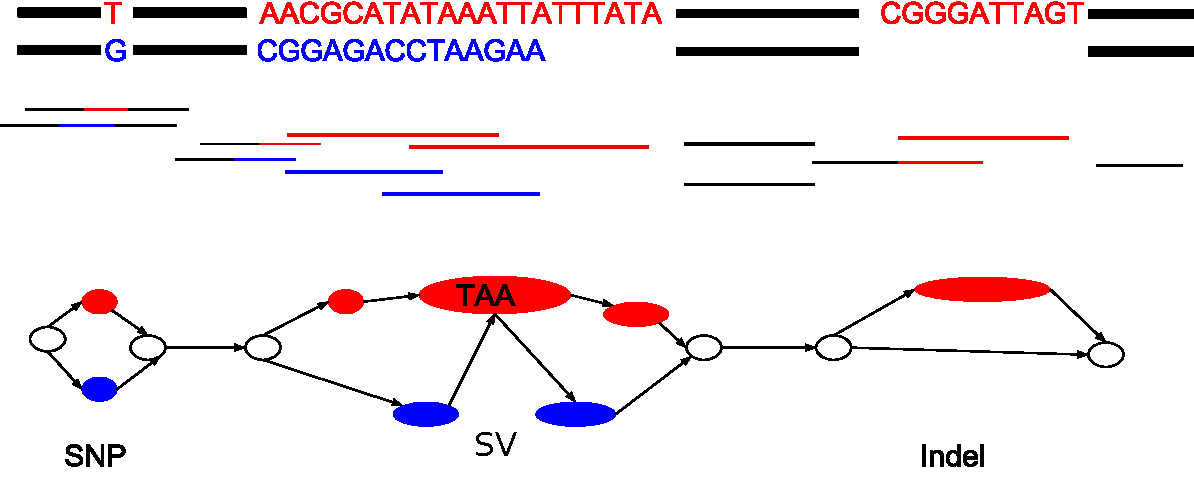
\includegraphics[width=\columnwidth]{ex_sv.pdf}
\caption{Given the input reads (middle) from the two sequences (top), we show a corresponding assembly graph at the bottom.
The bubbles in the sequence graph (bottom) show three different heterozygous variations; the first one is an SNV, the second one is an SV, and the third one is an indel. }
\label{fig:ex_sv}
\end{figure}

\paragraph{De Bruijn graphs}
% https://genome.sph.umich.edu/w/images/b/b4/666.2012.01.pdf
In this type of assembly graph, each read is broken into a sequence of overlapping k-mers. The distinct
k-mers are added as vertices to the graph, and k-mers that originate from adjacent positions in
a read are linked by an edge.
In Figure~\ref{fig:assembly_graphs}a, the reads are divided into words of fixed length $k$, where $k=4$. Here,
each node in the graph is a word and the connection between the nodes is based on the overlap between nodes.
Basically, the de Bruijn graph is a directed graph representing overlaps
between sequences of symbols, named after Nicolass Govert de Bruijn \citep{todd1933combinatorial}. Given an
alphabet $\sigma$ of $n$ symbols, a $k$ dimensional de Bruijn graph has the following properties.
\begin{enumerate}
 \item $n^k$ vertices produced by all words of length $k$ from alphabet $\sigma$
 \item Two vertices X and Y are connected if and only if the $k$ - 1
suffix of X is equal to the $k$ - 1 prefix of Y.
\end{enumerate}

The first application of the de Bruijn graph in genome assembly was introduced into
the EULER assembler \citep{pevzner2001eulerian} in order to tackle assembly complexity. 
The assembly problem can then be formulated as finding a walk
through the graph that visits each edge in the graph once --- an Eulerian path problem.
Due to the repeats, it is hard to find the Euler path. 
In most instances, the assembler attempts to construct
contigs consisting of the unambiguous, unbranching regions of the graph.

\paragraph{De Bruijn graph and overlap graph}
The de Bruijn graph theoretically achieves
the same tasks that the overlap graph does, but in an efficient manner.
The de Bruijn graph became widely used when the short reads from NGS appeared. The OLC
approach did not scale well on the high number of sequences generated by NGS. The
use of the de Bruijn graph is very interesting for short read assembly for its ability to
deal with the high redundancy of such sequencing in a very efficient way. Indeed a k-mer
present dozens of times in the sequencing dataset appears only once in the graph. This
makes the de Bruijn graph structure not very sensible to high coverage, unlike
OLC. The de Bruijn graph was first proposed as an alternative structure \citep{pevzner2001eulerian} because it
was less sensible to repeats. Repeats that were problematic in the OLC, creating very
complex and edges heavy zones, are collapsed in the de Bruijn graph.

From the above, it follows that the assembly graphs contain the information about ordering of reads. 
We now discuss the special structures in assembly graphs, that can occur due to repeats and heterozygous regions.

\paragraph{Graph structures} There are mainly two types of structures (bubbles and repeats) that occur in the assembly graphs for diploid genomes.

\textit{Bubbles.}
Bubbles are defined as a set of disjoint paths that share the same start and end nodes.
Bubbles in the graph represent heterozygosity for the diploid organism.
Bubbles can contain simple SNVs with only one allele difference, or even large complex structural variations in the order of a few kilo-bases.  
Figure~\ref{fig:ex_sv} illustrates how the bubbles in an assembly graph can contain both small variants (SNPs and indels up to several dozen base-pairs in length) and large structural variants.
\begin{figure}[t!]\centering
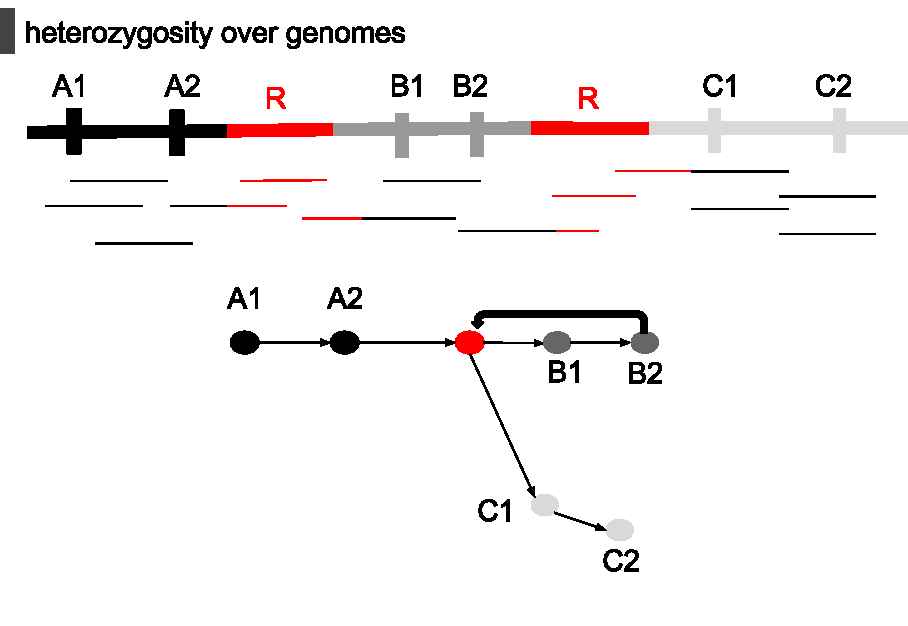
\includegraphics[width=\columnwidth]{repeats.pdf}
\caption{At the top, shown are the heterozygosity (in vertical bars) and repetitive regions (in red) over the genome. At the bottom, shown is the graph with nodes as heterozygous or repetitive region, and connections are based on the successive read overlap.
The graph has cycles because of repetitive region shown by R, which also causes two branches.}
\label{fig:repeats}
\end{figure}

\textit{Repeats.} The repeats over the genomes cause branches or cycles in the assembly graphs and, therefore, make a graph more complex and break its linear chain properties.
This is illustrated in Figure~\ref{fig:repeats}. In this example, the repeat $R$ causes cycles and branches in the graph.
Assemblers generally handle these repeats by making a guess as to which branch to follow.
Incorrect guesses create false joins (chimeric contigs) and erroneous copy numbers. 
If the assembler is more conservative, it will break the assembly at these branch points, leading to an accurate but fragmented assembly with fairly small contigs.
The maximal repeat resolution  depends on the read-length. If there is a read that is long enough to span the repeat region, then the repeat is resolvable.
Therefore, upcoming long-read sequencing technologies have the power to obtain maximal repeat-resolved diploid assemblies.

We have explored the assembly graphs and their special structures. We now provide the main approaches followed for reconstructing the genome from NGS data. 
\begin{figure}[t!]\centering
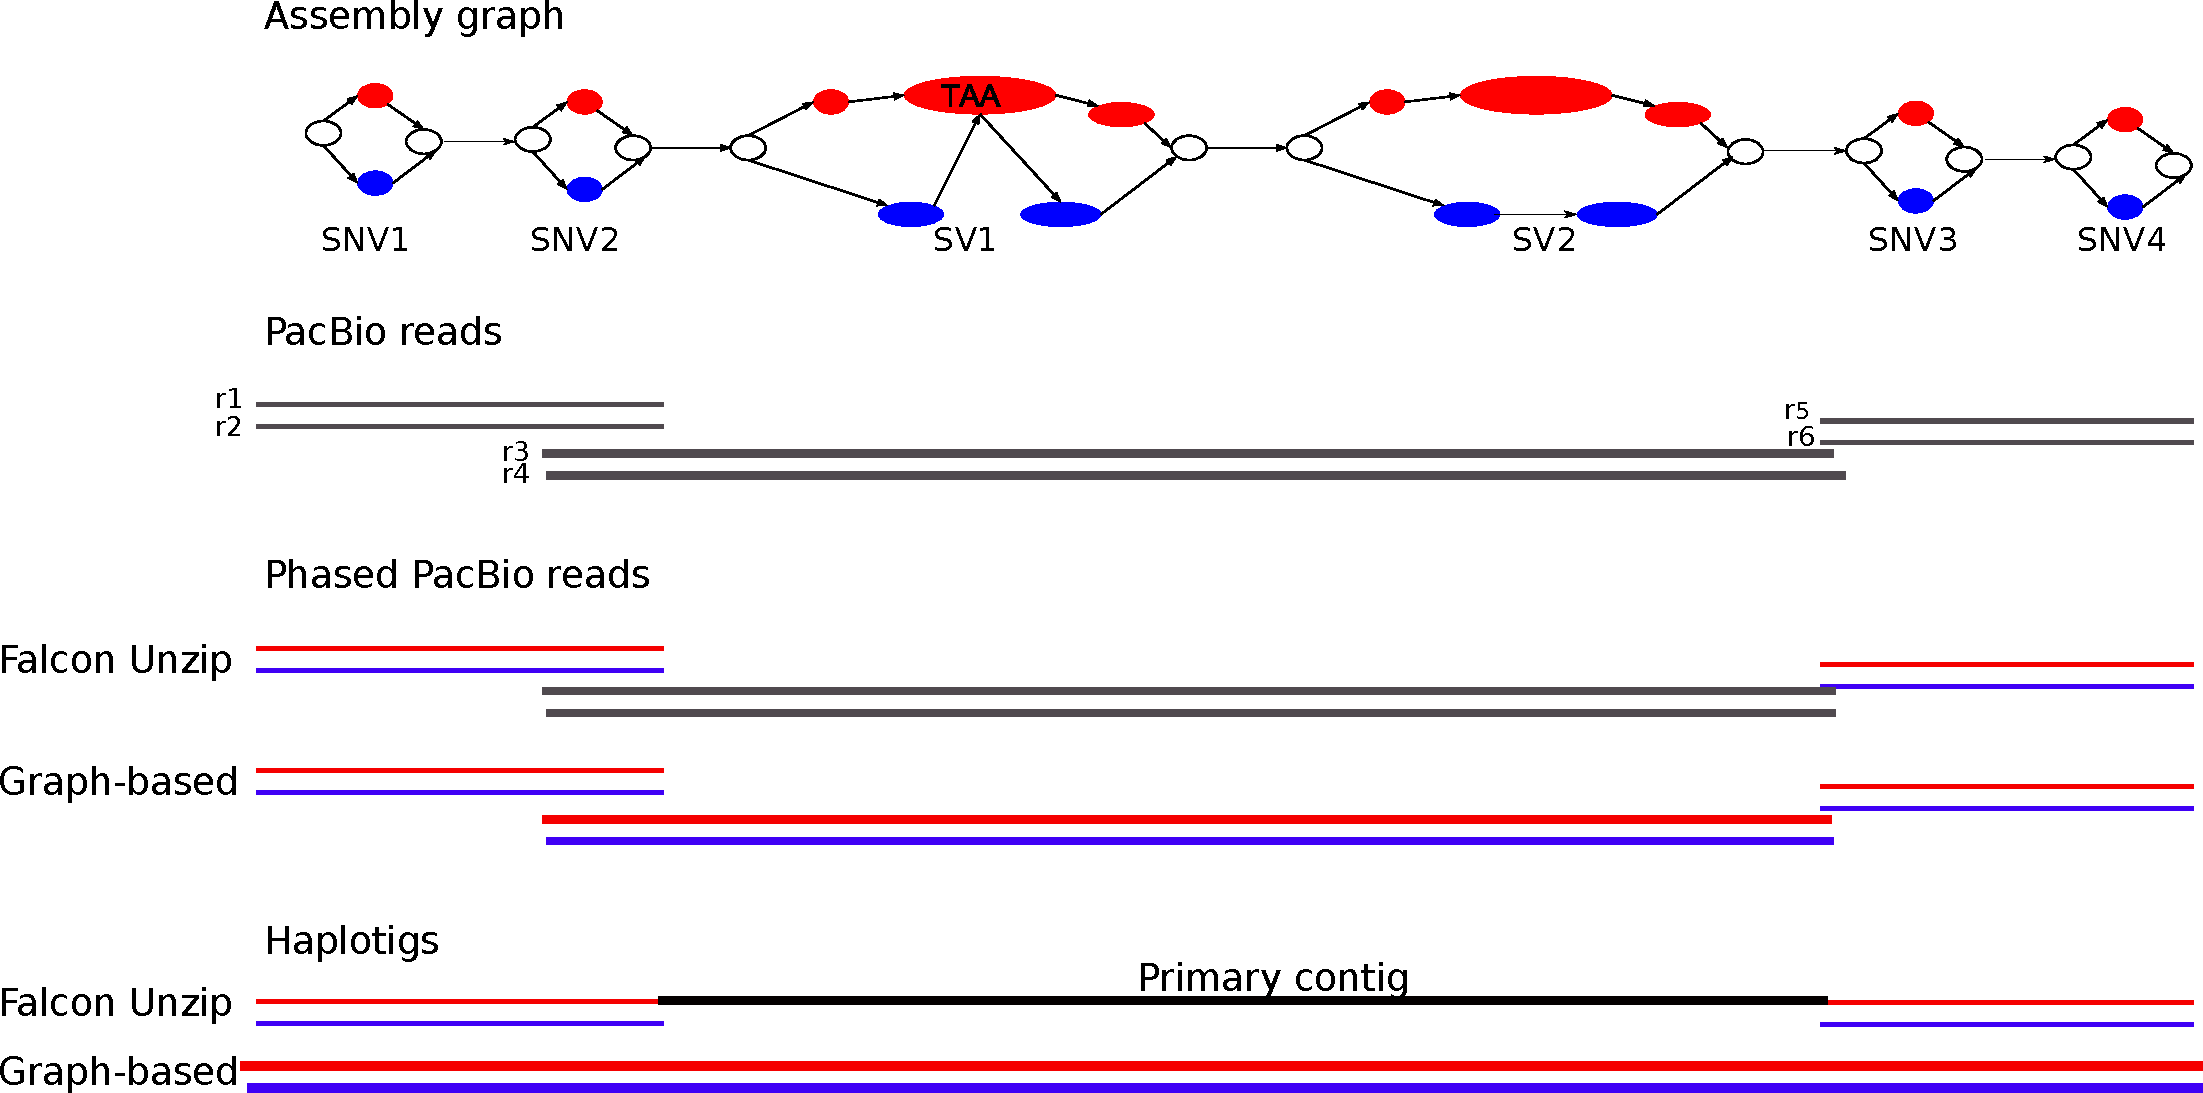
\includegraphics[width=\columnwidth]{ex_graph_approach.pdf}
\caption{Input: an assembly graph (top) (consisting of four SNVs and two SVs) and the PacBio reads $r_1, r_2, r_3, r_4, r_5, r_6$ (gray). 
Output: the phased reads (colored in blue and red) and haplotigs (bottom) using Falcon Unzip and our graph-based approach. Our graph-based phases central region, contrarily, Falcon Unzip does not.  }
\label{fig:ex_graph_approach}
\end{figure}

\subsection{Main approaches for diploid assembly}
Over the last decade, the development of various NGS technologies has impacted the assembly problem.
In theory, the problem of \textit{de novo assembly}---computing the consensus of two or more sequences---is NP-hard, when the problem is modeled either as string graphs or de Bruijn graphs \citep{medvedev2007computability}. 
There are several heuristic approaches to approximate the optimal de novo haploid assembly based on NGS datasets \citep{idury1995new, myers1995toward, myers2005fragment, pevzner2001eulerian, nagarajan2009parametric, nagarajan2013sequence, sovic2013approaches}.

However, even with Sanger (reads of the order of 800-1000 base pairs) and Illumina sequencing, which deliver short reads with low error rates, de novo assembly of heterozygous diploid genomes has been a difficult problem \citep{vinson2005assembly, levy2007diploid}.
In practice, there are several short-read assemblers based on Illumina data for heterozygous genomes \citep{kajitani2014efficient, pryszcz2016redundans, simpson2012efficient, bankevich2012spades, li2015fermikit}.
The assemblies that they produce are accurate, but contain gaps and are composed of relatively short contigs and scaffolds. 
Third generation sequencing technologies such as methods available from Pacific Biosciences (PacBio) and Oxford Nanopore Technologies (ONT) deliver much longer reads, but with high error rates.
There are now several long-read assemblers \citep{koren2017canu, vaser2017fast, xiao2016mecat, berlin2015assembling, chin2013nonhybrid, hunt2015circlator, lin2016assembly} that use these long-read data for de novo assembly.
The assemblies that are delivered from these assemblers are more contiguous, with longer contigs and scaffolds.
Finally, there are hybrid assemblers that take advantage of long-read data (with its high error rate) and short-read data (with its low error rate) \citep{bashir2012hybrid, antipov2015hybridspades, zimin2017hybrid} and attempt to combine the best aspects of both.
These hybrid assemblers have the power to deliver highly accurate, repeat-resolved assemblies.

The main drawback of above state-of-the-art assemblers is that they generate only one consensus sequence even for diploid organisms. To date, there is only one assembler that can produce diploid assemblies for diploid genomes.

\textit{Diploid assembly.} A recent and currently only available diploid assembly method --- Falcon Unzip \citep{chin2016phased} --- is purely PacBio based diploid assembler.
Falcon Unzip generates haplotype contigs or ``haplotigs'' that represent the diploid genome with correctly phased homologous chromosomes.
Falcon Unzip involves constructing a string graph from long PacBio reads, and generating haplotigs in a greedy manner using local conservative approach.


For generating haplotigs, Falcon Unzip first identifies phase for each read based on the condition that the read covers at-least one SNV for phasing.
In the regions over the genome where the SNVs are at a long distance to each other, the Falcon Unzip can not phase those regions, resulting in incomplete assemblies.
Additionally, the Falcon Unzip cannot phase all large structural variants and regions with high heterozygosity. 

% The pipeline is given in Figure~\ref{fig:falcon_unzip}.
% Falcon Unzip begins by using reads to construct a string graph that contains sets of ``haplotype-fused contigs'' , also called as ``primary contigs'', as well as bubbles representing divergent regions between homologous sequences (Fig.~\ref{fig:falcon_unzip}a). 
% Next, Falcon-Unzip identifies read haplotypes using phasing information from heterozygous positions that it identifies (Fig.~\ref{fig:falcon_unzip}b). 
% Phased reads are then used to assemble haplotigs and primary contigs (backbone contigs for both haplotypes) (Fig.~\ref{fig:falcon_unzip}c) 
% that form the final diploid assembly with phased single-nucleotide polymorphisms (SNPs) and structural variants (SVs).
% 
% \textit{Phasing using primary contigs.}
% In Falcon Unzip, the reads are aligned to primary contigs and heterozygous SNPs (het-SNPs) are called by analyzing the base frequency of the detailed sequence alignments.
% A simple phasing algorithm was developed to identify phased SNPs. 
% Along each contig, the algorithm assigns phasing blocks where ``chained phased SNPs'' can be identified. 
% Within each block, if a raw read contains a sufficient number of het-SNPs, it assigns a haplotype phase for the read unambiguously. 
% Combined with the block and the haplotype phase information, it assigns a ``block-phase'' tag for each phased read in each phasing block.
% Some reads might not have enough phasing information. For example, if there are not enough het-SNP sites covered by a read, it assigns a special 'un-phased tag' for each un-phased read.
% The initial assembly graph is fused using phased reads and the haplotigs are generated in a greedy manner using local conservative approach.
% % \todo{maybe add example how haplotigs from haplotype fused assembly graph works?}

% \begin{figure}[t!]\centering
% \includegraphics[width=\columnwidth]{{cropped_falcon-unzip}.pdf}
% \caption{(a) An initial assembly is computed by FALCON, which error corrects the raw reads (not shown) and then assembles them using a string graph of the read overlaps. 
% The assembled contigs are further refined by FALCON-Unzip into a final set of contigs and haplotigs. 
% (b) Phase heterozygous SNPs and group reads by haplotype. (c) The phased reads are used to open up the haplotype-fused path and generate as output a set of primary contigs and associated haplotigs.}
% \label{fig:falcon_unzip}
% \end{figure}

There is no known algorithm that works at different levels of heterozygosity, phases all types of structural variants and generates complete diploid assemblies.
A potential step to achieve this task of complete diploid assemblies is to phasing directly from the assembly graph.
Moreover, it becomes easier to detect large structural variants, such as translocations and other rearrangements, in an assembly graph.
Thus, working in the space of assembly graphs provides deep insights to detect all types of structural variation, which further helps in phasing whole genomes.

Additionally, the Falcon Unzip is purely PacBio based assembler, which uses very noisy data and, therefore, the Falcon Unzip requires high coverage data to producing accurate assemblies.
In contrast, hybrid approaches that combine accurate Illumina and long read PacBio data, conceptually have the potential to producing good quality assemblies even at low coverages.
However, there is no known algorithm, that combines mutiple sequencing datasets such as accurate Illumina and long read PacBio data, for producing good quality haplotigs.
\begin{gaps}
 Phasing bubbles directly from the assembly graph is an open problem. Additionally, the MEC formulation for phasing that works on graphs, by combining datasets from multiple sequencing technologies, is unknown. 
 \label{gap:gap4}
\end{gaps}

\begin{example}
Figure~\ref{fig:ex_graph_approach} demonstrates the conceptual advantages of our graph-based approach over the Falcon Unzip method.
Consider four SNVs separated by two large SVs and there are four reads spanning these variants.
Falcon Unzip can not phase the central region because the reads $r_3$ and $r_4$ do not cover any SNVs, resulting in incomplete haplotigs.
In contrast, the graph-based approaches attempt to detect all types of SVs and phase all of them.
\end{example}
Based on the above example, we observe that it is possible to deliver complete and contiguous haplotigs using assembly graph-based approach.

% \begin{figure}[t!]\centering
% 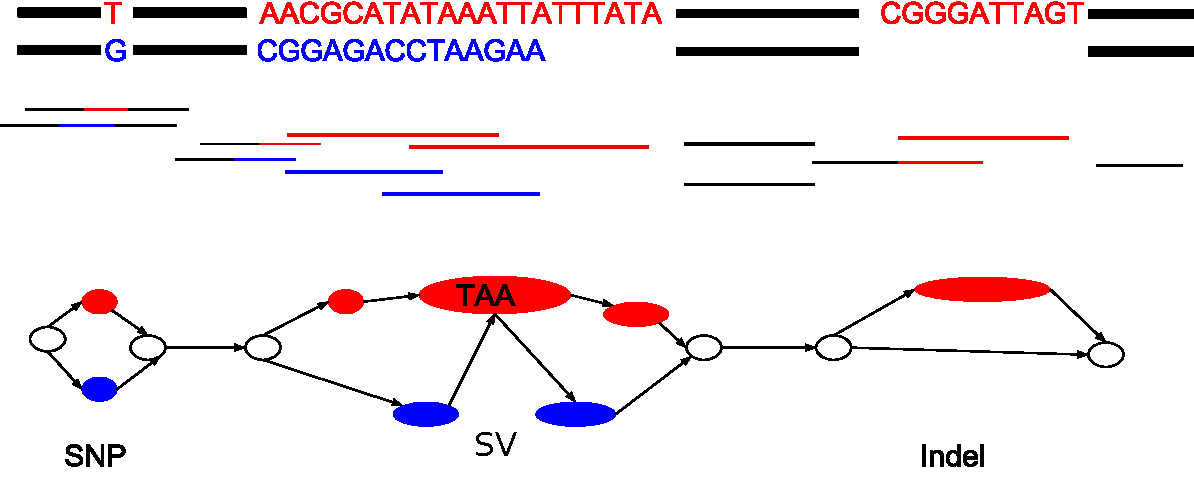
\includegraphics[width=\columnwidth]{ex_sv.pdf}
% \caption{Based on reads (middle) from the two sequences (top), the bubbles in the graph (bottom) show three different heterozygous structural variations; first is a SNV, second is a SV and third is an indel. }
% \label{fig:ex_sv}
% \end{figure}
\section{Outline of our contributions}
In the above section, I highlighted four ``open problems'' in the arena of haplotyping using NGS data.

\begin{itemize}
 \item In Chapter 2, I provide a general background on the different types of algorithms. I outline the motivation on how these algorithms are used in solving small daily examples fast. 
 I highlight the advantages and disadvantages of these algorithms in context of large problems.
 \item Solving MEC instances using NGS data are NP-hard. In Chapter 3, I describe the dynamic programming based algorithm to solve these instances approximately.
 I discuss the approximation guarantee, which provides hints that these instances can be solved in practice in polynomial time. (Problem~\ref{gap:gap1})
  \item In Chapter 4, I discuss different types of NGS datasets, with their advantages and disadvantages. I describe the integrative phasing framework obtained by combining NGS datasets. I discuss the parameterized algorithm that solves these instances efficiently in practice. 
  I demonstrate the effectiveness of this algorithm on real genomic datasets. (Problem~\ref{gap:gap2})
 \item In Chapter 5, I describe the generalized parameterized approach to incorporate information from pedigrees. I show the experiments on real datasets and highlight that pedigree data has an additional advantage in delivering better quality haplotypes. (Problem~\ref{gap:gap3})
 \item In Chapter 6, I describe the generalized approach --- haplotype-aware diploid assembly --- in a graph framework, that has the ability to handle all levels of heterozygosity and structural variations to produce accurate and complete haplotype assemblies.
 I present this approach as a hybrid of different types of NGS datasets and show its effectiveness on the pseudo-diploid genome. (Problem~\ref{gap:gap4})
 \item Finally, in Chapter 7, I provide a summary of the results presented in this thesis, along with the future outlook and perspectives.
\end{itemize}

\section{Relevant publications}
\begin{itemize}
 \item David Porubsky*, \underline{Shilpa Garg}*, Ashley D. Sanders*, V. Guryev, Peter M. Lansdorp, T. Marschall,
\textit{Dense And Accurate Whole-Chromosome Haplotyping Of Individual Genomes}, Nature Communications, 2017.

In this paper, my contribution was in developing an integrative pipeline and writing draft for WhatsHap section.
\item \underline{Shilpa Garg}, Marcel Martin and Tobias Marschall, \textit{Read-Based Phasing of Related Individuals},
Proceedings of ISMB 2016/Bioinformatics.
\item \underline{Shilpa Garg}, Mikko Rautiainen, Adam M Novak, Erik Garrison, Richard Durbin, Tobias Marschall, \textit{A graph-based approach to diploid genome assembly}, ISMB 2018 (to appear).
\item \underline{Shilpa Garg}, Tobias Moemke, \textit{A QPTAS for Gapless-MEC}, Submitted.
\item Preprint: M. Martin*, M. Patterson*, \underline{Shilpa Garg}, S. O. Fischer, N. Pisanti, G. W. Klau, A. Schnhuth, T.
Marschall, \textit{WhatsHap: fast and accurate read-based phasing}.

In this paper, my contribution was in developing some parts of the pipeline and making figures.
\end{itemize}


% \subsection{Issues we address}
% To address those problems, we will present new algorithmic approaches. 
% \begin{itemize}
% \item In the second chapter, we present the fundamental concepts of different type of algorithms.
%  \item In the third chapter, we present dynamic programming based algorithm to prove the near-polynomial approximation status of \GMEC.
%  \item In the forth chapter, we present a parameterized algorithm to solve \MEC instances integatively from different datasets.
%   \item In the fifth chapter, we present a integrative framework to solve sequencing-based and genetic haplotyping, helps to generate complete and accurate haplotypes.
%  \item In the sixth chapter, we introduce new way to represent the assembly graph and futher, finding long read paths in the graph based on different types of datasets, which futher helps in better phasing. 
% \end{itemize}


% 
% 
%  
% 
% \todo{cover these issues in approaches}
% \subsection{Diploid genome assembly hardness}
% \begin{itemize}
% \item Theoretical approximation gurantee on gapless-MEC. It is important because even for high coverages, we can solve it in polynomial time approximately.
%  \item integrating datasets to produce more accurarte and complete
%  \item non-reference denovo based, can not detect large SVs, directly from graph, hybrid
%  \item pedigree of genomes
% \end{itemize}
% 
% \subsection{Goals and achievements}
% \begin{enumerate}
%  \item DNA genomes ranging from small yeast like genome to larger ones like human.
%  \item end-to-end full genome sequences
%  \item efficient algorithms to generate optimal or near-optimal solution.
% \end{enumerate}
% 
% 
% 
% 
% \subsection{Outline of our contributions}
% \begin{enumerate}
%  \item Chpater 1 consists of ...
%   \item Chpater 2 consists of ...
%    \item Chpater 3 consists of ...
% \end{enumerate}







\chapter{Algorithmic Background}
% http://web.stanford.edu/group/hopes/cgi-bin/hopes_test/an-introduction-to-dna-and-chromosomes-text-and-audio/#what-is-dna-making-the-single-strand
% Various algorithms can be used for solving combinatorial optimization problems.
% As discussed in Chapter~\ref{ref:chp1}, the haplotyping problem can be formulated as a combinatorial optimization problem.
% Further, our focus here is on algorithms which are useful for solving the haplotyping problem using the Minimum Error Correction (MEC). 
% The MEC is known to be NP-hard \citep{Cilibrasi2007}.  
% The NP-hardness rules out the possibility for polynomial time exact algorithm under the assumption that $P \neq NP$.
% Nevertheless, we want to find the haplotypes. Therefore, we sacrifice the optimality condition and present a brief description of the category of algorithms that 
% find near-optimal solution and work well in practice. For some relevant instance classes (ie. bounded coverage), we can find optimal solutions.
% 
% 
% % The NP hardness is one of the most common characteristics of the vast majority of interesting computational biological problems.
% % The NP hardness rules out the existence of polynomial-time exact algorithms for these problems and thus making them ``intractable''.
% % % NP-completeness theory distinguishes computationally ``tractable'' problems,
% % % i.e., those solvable in deterministic polynomial time, from those problems that
% % % are classified as ``intractable'' by showing that they are NP-hard. 
% % Finding ways to deal with NP-hard problems is one of the central challenges in the field of computer science.
% % Thus, several types of algorithms have been developed, for instance, approximation algorithms, parameterized algorithms and randomized algorithms to cope with the intractability of computational problems,
% % In this chapter we provide basic fundamentals of these algorithms that can be used as tools to solve biological problems.
% % Furthermore, we explain these algorithms by using classic examples.
% % formulation for the diploid assembly problem and describe briefly various methods to perform haplotyping including graph-based approaches.
% % Furthermore, we discuss about the challenges to solve the problem and provide the main contributions of this thesis.
% \section{Overview}
% http://people.csail.mit.edu/rrw/presentations/marx-approx.pdf
Many computational problems that arise in practice from analyzing biological data sets are optimization problems.
For optimization problems, the goal is to minimize or maximize some objective function (e.g. cost, quality or other measures) over the set of possible solutions that satisfy some constraints.
These optimization problems often turn out to be NP-hard and, the
NP-hardness of an optimization problem implies that, unless P = NP, there is no polynomial-time algorithm
that finds the optimal value of the objective function. 
The next step would be to look for algorithms that provide near-optimal solutions and work fast in practice.
We therefore seek to understand the structure of relevant problem instances and to design algorithmic
techniques to exploit these structures.

To design and analyze algorithms for these optimization problems, we explore the theory of parameterized algorithms and the theory of approximation algorithms.
% In both the theories, the structures of different instances are analyzed that helps to design polynomial time algorithms.
Parameterized complexity aims to analyze problem instances in finer detail and some parameters are considered based on the structural and other properties of input or output.
The running time of parameterized algorithms is expressed as a function of these parameters. 
The goal is to identify the parameters for which the overall running time is small when their values are small, even if the input size is large. 
In approximation algorithms, we relax the optimality criterion: instead of looking for an exact optimal solution,
we allow solutions for which the objective function is close to the optimal solution within some worst case bound.
We guarantee that the quality of the approximate solution is not worse than that bound on the deviation of the solution from the optimum.
The approximation algorithms and the parameterized algorithms can be deterministic or randomized.

% Thus, designing algorithms whose run times are polynomial in the input size become feasible, under the scenario of relaxation in the condition of optimality, 
% in other words, accepting the approximate solutions.

\section{Types of algorithms}
In this thesis, we consider the following broadly defined categories of algorithms for solving computational problems: Parameterized algorithms, Approximation algorithms and Randomized algorithms.

\subsection{Parameterized algorithms}
Let us begin with a small example as illustrated by \cite{cygan2015parameterized}. 
Imagine that you are a security guard of a bar
in a small town of Germany. On Friday, several people come to the bar for a party. 
There are some people who often fight with each other at the bar and the guard takes note of them.
In order to have a peaceful party without any fights, the guard plans ahead and
only admits people who do not fight with anyone else at the
bar. At the same time, he is willing to reject at most $k$ people, such that he gains maximum profit.

The above situation can be formalized in the context of an optimization problem. Let us suppose that there are $n$ people who come to the bar, 
and the constraint is that for each pair of people, we know whether or not they will have a fight between them if the pair is allowed inside the bar. 
The goal here is to identify the number of people allowed inside the bar to incur maximum profit such that there are at most $k$ people who are prohibited.
Figure~\ref{fig:parameter_dia1} shows an instance of the problem and a solution for
 k = 3.  It can be easily checked that this instance has no solution with k = 2.
 
\begin{figure}[t!]\centering
\includegraphics[width=\columnwidth]{{parameter_dia1}.pdf}
\caption{An instance of the problem with a solution for k = 3. An edge between two guests means that they will fight if both are admitted. The grey circles represent the troublemakers.}
\label{fig:parameter_dia1}
\end{figure}
 
\paragraph{Efficient algorithms.}
Let us solve the above problem in a naive manner by trying all possibilities.
If the problem instance is small, i.e.\, $n=100$ people, then the number of possibilities are $2^{100}$.
Even for such a small instance, the algorithm takes a long time, and cannot give an answer in a reasonable amount of time.
Another approach to this problem is to reject a small number of guests, let's say, $k \le 10$.
In this case, the total number of possibilities are $100 \choose 10$. This approach is better compared to the brute-force approach, but even this approach takes a long time.

Let us look closer into the problem and, try to identify some peaceful people and troublemakers.
In particular, we want to identifying persons who do not have a conflict with anyone, and also identifying a person who fights with at aleast $k+1$ other persons.
The example for this case is shown in Figure~\ref{fig:parameter_dia1}. 
There are seven persons shown by nodes and there is an edge between nodes if the two persons fight between each other.
Here, we want to find a person that fights with at aleast four persons for $k=3$. In this example, the person whom we want to reject from the party is D, reducing $k$ by one.
We proceed ahead in a similar manner. If we are left with no such person then we know that each remaining person will fight with at most $k$ other persons.
Thus rejecting any single person resolves at most $k$ potential conflicts.
If there are more than $k^2$ potential conflicts, then it is not possible to have a good party by rejecting only $k$ persons.
Taken together, the persons can be classified into two important classes; one, those who participate in at aleast one potential conflict and second, those who participate in at most $k$ conflicts. 
Thus, in total, there are at most $k^2$ potential conflicts, which results in $2k^2$ persons for whom it is unknown.
Now, if we try all possibilities of $2k^2 \choose k$, the running time is reduced compared to previous approach, but even this approach takes a long time.

After all above insights, the main observation to consider is that every conflict has to be resolved, and the only way to resolve a conflict is to refuse at least one of the two persons.
Let us suppose that there is a conflict between persons X and Y. 
If we add one of them, let's say X, to the list of persons to reject and, then repeat this process by rejecting at most $k-1$ persons.
If it succeeds, we get the solution, otherwise we remove the person X from the reject list and, instead try moving Y to the reject list and run this algorithm recursively.
If this succeeds, we get the solution and otherwise, it is not possible to solve this problem by rejecting at most $k$ guests.

To analyze the running time of this recursive algorithm, there are in total $O(2^k)$ recursion calls, $2^k$ leaves in the recursion tree.
Each recursion call can be solved in linear time $O(m+n)$, where $m$ is the total number of possible conflicts.
The good news is that this recursive algorithm gives a solution in a reasonable amount of time.
This algorithm runs in time $O(2^k \cdot k \cdot n)$, 
and is faster than the brute-force algorithm which takes $O(n^k)$ time.
% Therefore, it is possible to design an efficient algorithm after having good insights on the structures of the problem instances.


In the $O(2^k \cdot k \cdot n)$--- time algorithm, the combinatorial explosion is restricted to parameter $k$, i.e.\, the running time is exponential in $k$, but linear in $n$.
The main insight from the above example is that the problem instances can be solved in time polynomial in the input size, if we fix a parameter. 
We aim to identify a parameter that is small for the problem instances encountered in practice.

We are now ready to provide some formal definitions on parameterized algorithms as defined by \cite{cygan2015parameterized}.

\begin{definition}[Parameterized algorithms]
 Algorithms with running time $f(k)\cdot n^c$, for a constant $c$ independent of both $n$ and $k$, are called \textit{fixed-parameter (FPT) algorithms}.
 \end{definition}
 
  Typically, the goal in parameterized algorithms is to design FPT algorithms, trying to make both $f(k)$ factors 
 and the constant $c$ in the bound on the running time as small as possible. 
 
 In parameterized algorithms, $k$ is simply a \textit{relevant secondary measurement} 
 that encapsulates some aspect of the input instance, be it the size of the solution or the structure and other characterizes of the input instance.


\paragraph{The art of parameterization.}
We have seen that we can solve a complex problem in an efficient manner by cleverly framing an algorithm using relevant parameters.
For some problem instances, it is easy to find such parameters, whereas it is difficult for others.

For example, let us consider a variant of the problem described above where we want to reject at most $k$ persons
such that the number of conflicts are at most $l$.
Based on the properties explicitly given in the input instance, the first guess is to parameterize either by $k$, by $l$ or both. 
In case of both parameters, the goal is to find an FPT algorithm with running time $f(k,l) \cdot n^c$ for some computable function $f$
depending only on $k$ and $l$. Thus, the above definition for a single parameter can be extended to considering a set of parameters at the same time.

Parameterized algorithm (more than one parameter): Formally, one can express parameterization by $k$ and $l$, by defining the value $k+l$ to be the parameter:
an $f(k,l)\cdot n^c$ algorithm exists if and only if an $f(k+l) \cdot n^c$ algorithm exists.

Other variants of the problem described above could be formulated as identifying at most $k$ persons to reject such that,
say, the numbers of conflicts decreases by $p$, or such that each allowed person conflicts with at most $d$ other persons,
or such that the average number of conflicts per guest is at most $a$. Based on the properties of this instance, the parameters $p, d, a$ are again explicitly given in the input,
indicating the kind of solution to find. 

The bottom-line is that we can find different parameters for a problem based on the structure and other special properties of problem instances.
This allows us to algorithms which are exponential in these parameters, but polynomial in the input size.

Different problem domains offer different choices of suitable parameters. For example, 
for the string or sequence problems that are related to genomics, one can parameterize by the maximum read length, by the maximum coverage,
by the size of alphabet or by the number of alleles in a variant.

Parameterized complexity allows us to study how different parameters influence the time complexity of the problem.
Additionally, it allows us to solve the problem effiicently.
% A successful parameterization of a problem needs to satisfy two properties:
% First, there should be specific reason for the choice of parameters for different applications.
% Second, we need efficient algorithms where the combinatorial explosion is restricted to the parameter(s), that is, we want the problem to be in FPT with this parameterization.

In conclusion, for the same problem, there can be multiple choices of parameters. 
Selecting the right parameter(s) for a particular problem is often not straightforward.

% \subsubsection{Formal definitions}
We follow the formal foundation of parameterized complexity by \cite{cygan2015parameterized}.

\begin{definition}
 A parameterized problem is a language $L \subseteq \sum^* \times \N$, where $\sum$ is a fixed, finite alphabet. For an instance $(x,k) \in \sum^* \times \N$, $k$ is called the parameter.
\end{definition}

% The size of an instance $(x,k)$ of a parameterized problem as $|x| + k$. 
%  One interpretation of this convention is that, when given to the algorithm on the input, the parameter $k$ is encoded in unary.


\begin{definition}
 A parameterized problem $L \subset \sum^* \times \N$ is called \textit{fixed-parameter tractable} (FPT) if there exists an algorithm $\mathcal{A}$ (called a fixed-parameter algorithm),
 a computable function $f: \N \rightarrow \N$ and a constant $c$ such that, given $(x,k) \in \sum^* \times \N$, the algorithm $\mathcal{A}$ correctly decides
 whether $(x,k) \in L$ in time that is bounded from above by $f(k) \cdot |(x,k)|^c$, where $|(x,k)|$ is the size of an instance.
 The complexity class containing all fixed-parameter tractable problems is called FPT.
\end{definition}

Observe that, given some parameterization problem $L$, the algorithm designer has essentially two different optimization goals when designing FPT algorithms for $L$.
Since the worst case time complexity has to be of the form of $f(k)\cdot n^c$, one can:
\begin{itemize}
 \item optimize the \textit{parametric dependence} of the running time, i.e., try to design an algorithm where function $f$ grows as slowly as possible; or
 \item optimize the \textit{polynomial factor} in the running time, i.e. try to design an algorithm where constant $c$ is as small as possible.
\end{itemize}

\subsection{Randomized algorithms}
In randomized algorithms, the idea is to perform independent random choices and then utilize these random choices to influence the computation.
The assumption is that the average over all random choices results in good performance.
% For example, sample a random element from a set $X$ by choosing $O(\log |X|)$ random bits and then use these
% bits to index an element in the set. 

There are two principal advantages to using randomized algorithms. The first is performance --- for many problems, 
randomized algorithms run faster than the best known deterministic algorithms.
Thus, randomized techniques are often used in approximation theory in order to provide a faster solution to the problem.
Second, many randomized algorithms are simpler to describe and implement than deterministic algorithms of
comparable performance. 

An observation from basic probability theory ---\textit{linearity of expectation}--- that is often used in the analysis of randomized algorithms.
Linearity of expectation states that the expectation over a sum of random variables is equal to the sum over the expectation of each random variable.
For example, for random variables, $X_1, X_2 \ldots$, the linearity of expectation is given by.
\begin{equation}
 E\big[\sum_i X_i\big] = \sum_i E[X_i].
\end{equation}
% https://www.cs.cmu.edu/afs/cs/academic/class/15451-s07/www/lecture_notes/lect0123.pdf
Here we provide an example of a randomized version of Quick-sort for illustration. 
Quick-sort is a sorting technique which proceeds as follows.
Pick an element $p$ of the array as the pivot.
Reorder the elements of the array such that all the elements with values smaller than the pivot are to the left and the greater ones are to the right. After the reordering operation is finished, the pivot is at its final position.
The next step is to recursively apply the above steps of randomly picking the pivot and reordering to the left and right parts.

Quick-sort depends on how the pivot element is picked.
If the pivot element is chosen randomly, then it is known as randomized Quick-sort.
For any given array $A$ of size $n$, it is easy to show that the expected time of this algorithm is $O(n \log n)$ using the linearity of expectation \citep{motwani2010randomized}.
% This is called a Worst-case Expected-Time bound, which is better than an average-case bound because we are no longer assuming any special properties
Making the algorithm probabilistic gives us more control over the running time.
The algorithm runs fast with high probability. They are simple and efficient compared to deterministic algorithms.
% We talk about Note that we are not talking about worst case runtimes here (in this sense, randomized algorithms are an outlier in your exposition).
% As illustrated by \cite{motwani2010randomized}, let us consider the example of \textit{binary planar partition} of a set of $n$ disjoint line segments in the plane.
% The goal is to build a small linear decision tree that has at most one line segment or its pieces in each cell.
% This problem can be represented by a binary tree.
% Every internal node of a tree has two children. The children of each node $v$ of a tree represent the associated regions $r(v)$ of the plane.
% Associated with each internal node $v$ of a tree is a line $l(v)$ that intersects $r(v)$.
% The region corresponding to the root is the entire plane.
% The region $r(v)$ is partitioned by $l(v)$ into two regions $r_1(v)$ and $r_2(v)$,
% which are the regions associated with the two children of $v$. Thus, any region $r$ of the partition
% is bounded by the partition lines on the path from the root to the node corresponding to $r$ in the tree.
% % \todo{think of better real-world example than in computer graphics.}
% 
% \begin{figure}[t!]\centering
% \includegraphics[width=\columnwidth]{{random_dia1}.pdf}
% \caption{An example of a binary planar partition for a set of segments (dark lines). Each leaf is labeled by the line segment it contains. The labels r(v) are omitted for clarity.}
% \label{fig:random_dia1}
% \end{figure}
% 
% Given a set $S = \{s_1, s_2, \ldots, s_n\}$ of non-intersecting line segments in the plane,
% we wish to find a binary planar partition such that every region in the partition contains at most one line segment.
% Notice that the definition allows us to divide the input line segment $s_i$ into several segments $s_{i1}, s_{i2}, \ldots,$
% each of which lies in a different region. The example shows such a partition of a set into three line segments in Figure~\ref{fig:random_dia1}.
% 
% For a line segment $s$, let $l(s)$ denote the line obtained by extending $s$ on both sides to infinity.
% For the set $S = \{s_1, s_2, \ldots, s_n\}$ of line segments, a simple and natural class of partition 
% is the set of autopartitions, which are formed by only using lines from the set $\{l(s_1), l(s_2), \ldots, l(s_n)\}$
% in constructing the partition. 
% 
% In the algorithm, the input is the set $S = \{s_1, s_2, \ldots, s_n\}$ of non-intersecting line segments.
% The output is the binary autopartitions of $S$. To solve it, we pick a permutation $\pi$ of $\{1,2, \ldots, n\}$ uniformly
% at random from the $n!$ possible permutations. Then we cut it with $l(s_i)$ where $i$ is first in the ordering $\pi$
% such that $s_i$ cuts the region. We repeat this process till a region contains more than one segment.
% 
% For the analysis of randomized algorithm, we show that the expected size of autopartitions produced by the algorithm is $O(n \log n)$.
% We can easily show this using linear of expectation of the intersections.

% http://math.mit.edu/~goemans/18434S06/knapsack-katherine.pdf
\subsection{Approximation algorithms}
% Most of the real-world problems can be modelled as optimization problems and unfortunately, most interesting discrete optimization problems are NP-hard.
% Thus unless P=NP, there are no efficient algorithms to find optimal solutions to such problems. We define an efficient algorithm is the one that is solved in time polynomial in input size.
% What should we do next? How about we find a near-optimal solution which can be found in polynomial time? Furthermore, we focus on finding 
% polynomial-time algorithms for some special cases of the problem, instead of any instance.
In this section, we present some fundamental definitions and concepts of approximation algorithms.
% Informally, an NP-Optimization problem $X$ is either a minimization or a
% maximization problem. $X$ defines a set of valid instances, and for each instance
% $I$, a non-empty set of feasible solutions. Moreover an objective function value is
% defined that, for each feasible solution $S$, returns a non-negative real number,
% which is generally intended as a measure of the quality of the solution. The
% goal is either to maximize or minimize the objective function value, and we call
% $X$ a maximization problem or a minimization problem, accordingly. A solution
% $OPT$ that maximizes (respectively minimizes) the objective function value is
% called optimal solution; for the problems that we are interested in, finding an
% optimal solution is NP-hard. For simplicity, from now on we talk about
% optimization problems. 
Approximation algorithms are a techniques for finding approximate solution for optimization problems that are NP hard.
If the approximate solution is close enough to the optimal solution and the algorithm runs faster, then this behavior might be preferable for most practical purposes. 
Based on this motivation, we define the notion of $\alpha$-approximation.

We follow the basic definitions of \cite{vazirani2013approximation}.

\begin{definition}
 A polynomial-time algorithm $A$ for an optimization problem $X$
is an $\alpha$-approximation algorithm ($\alpha \ge 1$) if it returns a feasible solution whose value is
at most a factor $\alpha$ away from the value of the optimal solution, for any input
instance.
\label{def:apx}
\end{definition}

Thus, if $opt$ is the optimal value of the objective function, an algorithm is an $\alpha$-approximation if it always returns a
solution whose value is at most $\alpha \cdot opt$ for a minimization problem, or at least
$opt/\alpha$ for a maximization problem.
In general, $\alpha$ can be a growing function of the input size, and does not necessarily need to be a constant number.
For some problems, it is possible to find approximate solutions that are
arbitrarily close to the optimal solution. More formally:

\begin{definition}
 We say that an algorithm $A$ is a polynomial time approximation
scheme (PTAS) for an optimization problem $X$ if for every fixed $\epsilon$ > 0 and for
any instance $I$, the running time of $A(\epsilon, I)$ is polynomial in the input size $n$,
and it returns a solution whose value is at most a $1 + \epsilon$ factor away from the
value of the optimal solution.
\label{def:ptas}
\end{definition}

%  \begin{figure}[t!]\centering
% \includegraphics[width=.6\columnwidth, height=.5\columnwidth]{{approx_dia1}.pdf}
% \caption{An instance of Vertex Cover problem. An optimal vertex cover is {b, c, e, i, g}.}
% \label{fig:approx_dia1}
% \end{figure}

Definitions~\ref{def:apx} and~\ref{def:ptas} can be generalized in the context of randomized algorithms.
In particular, we call an algorithm an expected
$\alpha$-approximation if the expected value of the output solution satisfies the above
constraints.

For a PTAS, the running time is polynomial for a fixed $\epsilon$, but the dependency
on $\epsilon$ can be arbitrary; in fact, running times can be on the order of $f(1/\epsilon)n ^{O(g(1/\epsilon))}$ for some functions $f$ and $g$ that are super-polynomial with
respect to $1/\epsilon$. Based on these functions $f$ and $g$, there are different variants of PTAS algorithms.
If the function $g$ is a constant that does not depend
on $\epsilon$, the algorithm is called Efficient PTAS (EPTAS); if, moreover, $f$
is polynomial in $1/\epsilon$, then it is called a Fully Polynomial Time Approximation
Scheme (FPTAS). In some sense, NP-hard problems admitting an FPTAS can
be thought as the easiest hard problems; one such example is the Knapsack
Problem.

A relaxation of Definition ~\ref{def:ptas} that allows for a
slightly larger running time is a Quasi-Polynomial Time Approximation Scheme
(QPTAS). A QPTAS is defined exactly same as above, except that $A$ is allowed quasi-polynomial
time $O(n^{poly \log n})$.

The class of problems that admit a constant factor approximation in polynomial time is called
APX. Clearly, all problems that admit a PTAS are in APX, but the converse
is not true if $P \neq NP$ \citep{jansen1998introduction}.

Some problems are known to be APX-hard. If a problem is APX-hard, then
the existence of a PTAS for it would imply the existence of a PTAS for every
problem in APX. Thus, being APX-hard is considered a strong evidence that
the problem does not admit a PTAS.

The existence of a QPTAS for a problem is sometimes seen as a hint that a
PTAS might exist: in fact, it implies that the problem is not APX-hard.

For some problems, we can obtain better approximation ratios if we assume
that the solution is large enough. Formally, for a minimization problem $X$, the
asymptotic approximation ratio $\rho$ of an algorithm $A$ is defined as:
\[
\rho = lim_{n \rightarrow \infty} sup_I \{ apx(I)/opt(I): opt(I) \ge n \}
\]

where $apx(I)$ and $opt(I)$ are the objective function value computed by algorithm $A$ and optimal value solution on the instance $I$ respectively.
Similarly to the definition of PTAS, we say that an algorithm $A$ is an
Asymptotic PTAS or APTAS for problem $X$ if $A(\epsilon, .)$ is an asymptotic $(1 + \epsilon)$-approximation for any fixed $\epsilon > 0$.

There are several advantages to using approximation algorithms.
 \begin{itemize}
  \item An approximation algorithm provides a way to find a near-optimal solutions when the optimal solution is not required, and finding an optimal solution for the problem is NP hard.
%   \item An approximation algorithm gives us an idea about how to devise a heuristic that will perform well in practice for the actual problem.
  \item An approximation algorithm provides a mathematically rigorous basis to study heuristics, and helps in unraveling structures of problem instances.
  \item The field of approximation algorithms gives us a means of distinguishing between various optimization problems in terms of how well they can be approximated.
 \end{itemize} 
%  https://web.cs.ship.edu/~tbriggs/dynamic/
Let us consider a classic example to illustrate the motivation and design of an approximation algorithm. 
Imagine that a thief has entered a house when its inhabitants have gone on a vacation.
The thief has a knapsack which is of fixed weight. In the house, the thief has multiple options for valuable items to steal.
Each of these items has a fixed price and weight as shown in Table~\ref{table:knapsack}. 
Since the knapsack that can carry a fixed weight of 12, the thief can not steal all the items. 
The thief's goal is to steal the items such that he gains the maximum profit from the items that fit into his knapsack. 
The thief problem actually is the popular Knapsack Problem.
\begin{center}
\begin{table}
\centering
\begin{tabular}{ lccc } 
 \hline
 Item & weight & price \\ 
  \hline
 gold ring & 3 & 20 \\
 mobile & 8 & 10 \\
 radio & 4 & 8 \\
 shoes & 5 & 3\\
 \hline
\end{tabular}
\\[10pt]
 \caption{Example for Knapsack problem}
\label{table:knapsack}
\end{table}
\end{center}
\paragraph{Efficient algorithms.}
The naive approach that a thief thinks of, is to try all possibilities of items and then choose the best.
The total number of possible combinations are $2^n$, which takes long time to compute the final solution. 

The next approach the thief follows is sorting the items in non-decreasing order based on the price.
The thief would first include an item in the knapsack with the maximum price and so on.
In this example, the thief first takes the gold ring and then, the mobile phone, which results in a weight of 11 and a price of 30.
This approach is basically a greedy approach and does not always give the optimal solution. 
For instance, in this example, the optimal solution consists of items 1, 3 and 4, for a total weight of 31.

Another technique that the thief can employ is dynamic programming. 
The thief considers sub-problems based on different items.
The thief stores the information ``the best knapsack so far'' for these sub-problems in a DP table.
The main idea is that the thief does not have to re-compute some sub-problems, which helps to save time.

% The main difference of DP algorithm to previous greedy approach is seen at processing the third item. 
% First, notice that the best knapsack that can consist, up until size four, does not include the third item. 
% Then, when the capacity of the knapsack increases enough to hold the third item, 
% the value changes --- the value of the knapsack now includes the second and third items, for a total value of 30. 
% Finally, when the capacity is large enough to hold all three items, then the capacity is grown to hold all three items. 
% However, following the same pattern for the fourth item, it is clear that algorithm works by showing that including the fourth item in place of any other item is not required.

\textit{Running time.} The run-time of this approach depends on the size of the DP table. 
Its two factors are $k$ rows (determined by the target capacity), and the $n$ columns (the number of items in the set). So, the run-time is $\theta(k \dot n)$. 
The main point here is that $k$ is not a constant, and its size may be considerably larger than the number of items $n$ in the set. 
Therefore, it is inefficient to solve this problem using a deterministic algorithm.
However, these instances often arise in practice and we would like to solve them. 
Thus we want to look into its approximate solution such that the algorithm to generate this solution is faster than a deterministic algorithm.

We now provide its formal definition and its approximate solution.

In the knapsack problem, given a knapsack of size $B \in Z^+$ and a set $S = \{a_1, . . . , a_n\}$
of items with their corresponding sizes and profits $s(a_i) \in Z^+$ and $p(a_i) \in Z^+$, the goal is to find
an optimal subset of objects whose total size is bounded by $B$ and which yields the maximum possible
total profit. This problem is also called as the 0/1 knapsack problem because each
item can either be included in or excluded from the knapsack. 

\paragraph{PTAS for Knapsack.}
We present an algorithm, which was proposed by \cite{lawler1979fast}, where it is assumed that we know the optimal solution $OPT$.
Let us assume that the set $O \subset S$ is considered by the optimal solution.
Another set $Q \subset O$ contains the items with value $\ge \epsilon \cdot OPT$.
We try all possibilities for sets $Q$ such that $|Q| \le 1/\epsilon$.
For some $Q$ we remove an item from a set with value $\ge \epsilon \cdot OPT$ and then run greedy algorithm to obtain set $G$.
The final solution is the best value obtained by the union of $Q$ and $G$.
The running time of this algorithm is $(n+1)^{1/\epsilon} \cdot \poly(n)$.

For analyzing this algorithm, let us consider a case when $Q$ is guessed correctly, then the loss from greedy algorithm is at most $\epsilon \cdot OPT$.
This happens due to the bound on the size on items that are removed, which are bounded by $\epsilon \cdot OPT$.
Therefore, it is easy to see that $p(Q \cup G) = OPT - \epsilon \cdot OPT = (1-\epsilon)OPT$.
% A clever approach involves utilizing jointly the brute-force and greedy method, meaning, using brute-force of part of the solution and
% then using the greedy algorithm on the rest. In particular, consider all $O(n^k)$
% possible subsets of $k$ items from $n$ items, where $k$ is some fixed constant.
% Then for each subset, use the greedy algorithm to fill up the rest of the knapsack in $O(n)$
% time. Let us suppose that the most profitable subset is $A$. The total running time of this algorithm is thus
% $O(kn^{k+1})$. If $O$ is the optimal subset, then the resulting approximation $P(A)$ achieves
% \[
% P(O) \leq P(A)(1+1/k) 
% \]
% 
% The above statement can be shown using the following insights.
% 
% It is straightforward to see that this algorithm returns the optimal solution if the optimal set $O$ has size less than or equal to $k$.
% Otherwise, let
% $H = \{a_1, . . . , a_k\}$ be the set of $k$ most profitable items in $O$. Since all subsets of size $k$ items
% are considered in the brute-force step, $H$ must be one of them. For this subset, filling in the
% rest of the knapsack using the greedy algorithm will yield a profit that satisfies the desired
% bound.
% 
% Let $L1 = O \setminus H = \{a_{k+1}, . . . , a_x\}$, and order the remaining items in $O$ in decreasing order of ratio
% of profit density. Let $m$ be the index of the first item in $L1$ which is not picked by the
% greedy algorithm step after picking $H$ in the brute-force step. The reason the item $a_m$ is
% not picked is that its size is larger than the remaining space $B_e$ in the knapsack. This also
% indicates that the greedy algorithm step has only picked items that have profit density of at
% least $p(a_m)/s(a_m)$ because it picks items in decreasing order of profit density. At this point,
% the knapsack contains $H, a_{k+1}, \ldots , a_{m-1}$, and some items not in $O$.
% 
% Let $G$ be the items packed by the greedy algorithm step. As mentioned before, all items
% in set $G$ have profit density of at least $p(a_m)/s(a_m)$. The items in $G \setminus O$, or the items in $G$
% that are not in the optimal set $O$, have total size
% \[
% \delta = B - (B_e + \sum_{i=1}^{m-1} s(a_i))
% \]
% 
% Since all the items have profit density of at least $p(a_m)/s(a_m)$, we can bound the profit of $G$:
% \[
% P(G) \geq \sum_{i=k+1}^{m-1} p(a_i) + \delta p(a_m)/s(a_m)
% \]
% 
% We can write the total profit of the items in $O$ as:
% \[
% P(O) = \sum_{i=1}^k p(a_i) + \sum_{i=k+1}^{m-1} p(a_i) + \sum_{i=m}^{|O|} p(a_i)
% \]
% 
% Using simple calculations, it can be shown that 
% \[
% P(O) \textless P(H \cup G) + p(a_m)
% \]
% 
% The best-found subset of items $A$ returned after both the brute-force and the greedy algorithm
% steps will have at least as much profit as that of $H$ and $G$ in combination, since we know that the
% union of $H$ and $G$ must have been one of the considered subsets. 
% Since $P(O) \textless P(H \cup G) + p(a_m)$ and $P(A) \geq P(H \cup G)$, then $P(O) - P(A) \textless p(a_m)$. Because the $k$ items in $H$ all
% have profit at least as large as that of $a_m$, we have that $s(a_m) \leq S(O)/(k + 1)$, and this gives
% the approximation ratio.
% To obtain the polynomial time approximation scheme or PTAS, we have a $(1 - \epsilon)$ approximation
% where $1/\epsilon = k + 1$. The resulting running time is $O(1/\epsilon \cdot n^{1/\epsilon})$, so the approximation
% scheme is polynomial in $n$ but not $1/\epsilon$. 

The above analysis shows that the Knapsack problem is in PTAS. In addition, the problem exhibits full polynomial time approximation scheme (FPTAS).

% \section{Discussion}
% In this chapter, we have explored different types of algorithms such as parameterized, randomized and approximation algorithms using classical examples.
% With this background chapter on algorithms, we set up a good foundation to solving the phasing problem that is explained in subsequent chapters.

%  Let us consider an example of vertex cover in Figure~\ref{fig:approx_dia1} to explain approximation algorithm. 
% %  https://www.cs.dartmouth.edu/~ac/Teach/CS105-Winter05/Notes/wan-ba-scribe.pdf
% Given a $G= (V,E)$, find a minimum subset $C \subset V$, such that $C$ \textit{covers} all edges in $E$, i.e., 
% every edge $\in E$ is incident to at least one vertex in $C$.
% 
% We consider the following steps to solve this problem. Let us consider set $C$ as empty. 
% We pick any edge $\{u,v\} \in E$ and add it to the set $C$. Afterwards we delete all the edges incident to either $u$ or $v$.
% We repeat this process till $E$ is not empty.
% 
% The above algorithm is a 2-approximation for vertex cover problem.

% An approximation algorithm, by definition, proves that a certain approximation
% factor is possible for a problem; thus, it provides an upper bound on the best
% possible approximation factor.
% A significant amount of research has been devoted to proofs
% that certain approximation ratios are not possible (under the assumption that
% $P \neq NP$ or analogous assumptions). These results provide a lower bound on
% the approximation factor.
% 
% Stronger results can often be provided by making stronger assumptions;
% for example, many hardness results have been proven under the assumption
% that $NP \subseteq DTIME (n^{O(log log n)})$, or the stronger $NP \subseteq DTIME (n^{O(log log n)})$
% (that is, NP-hard problems cannot be solved in quasi-polynomial time); more
% ecently, hardness results have been proved under the Exponential Time Hypothesis
% (ETH), that is, the assumption that SAT cannot be solved in subexponential
% time. Another strong hardness assumption is the Unique Games
% Conjecture (UGC). Clearly, stronger assumptions
% might lead to stronger results, but they are also considered less likely to be
% true; hence, there is a strong push for results that are as strong as possible,
% while relying on the weakest possible assumption (ideally, $P \neq NP$).








\chapter{Approximation algorithm for phasing individual genomes}\label{ref:chp3}

In this chapter, we study the approximation status of \GMEC, which is a variant of \MEC problem (see Problem~\ref{prob:mec} introduced in Chapter~\ref{ref:chp1}).
In other words, the minimum error correction problem (\MEC) is closely related to segmentation problems that were introduced by {[}Kleinberg--Papadimitriou--Raghavan STOC'98{]} in the context of data mining.
A \MEC instance is an $n \times m$ matrix $M$ with entries from $\{0,1,-\}$. 
    Feasible solutions are composed of two binary $m$-bit strings, together with an assignment of each row of $M$ to one of the two strings.
    The objective is to minimize the number of mismatches (errors) where the row has a value that differs from the assigned solution string.
    The symbol ``$-$'' is a wildcard that matches both $0$ and $1$.
    A \MEC instance is \textit{gapless}, if in each row of $M$ all binary entries are consecutive.

     Without restrictions, it is known to be $\UG$-hard \citep{trevisan2012khot} to compute an $O(1)$-approximate solution to \MEC. 
     For both \MEC and \GMEC, the best polynomial time approximation algorithm has a logarithmic performance guarantee \citep{BDK+16_minimum}.
    We partially settle the approximation status of \GMEC by providing a quasi-polynomial time approximation scheme (QPTAS).
    Additionally, for the relevant case where the binary part of a row is not contained in the binary part of another row, we provide a polynomial time approximation scheme (PTAS).
    
%     \begin{figure}[t!]\centering
% \includegraphics[width=\columnwidth]{{classes}.pdf}
% \caption{Figure shows the relationship between different classes of problems. In red, we show the approximation status known for different versions of \MEC.}
% \label{fig:classes}
% \end{figure}

\section{Our results.}
Our main result is the following theorem.
\begin{theorem}\label{thm:qptas}
    There is a quasi-polynomial time approximation scheme (QPTAS) for \GMEC.
\end{theorem}
We therefore partially settle the approximability for \GMEC, which is not $\APX$-hard unless $\NP \subseteq \QP$ (cf.~\cite{RS09_approximation}).
Moreover, \cite{Cilibrasi2007} showed that allowing a single gap in each string renders the problem $\APX$-hard.
Thus our result reveals a separation of the hardness of the gapless case and the case where we allow a single gap.
Furthermore, already \BMEC is strongly $\NP$-hard since the input does not contain numerical values. 
Therefore we can exclude the existence of an FPTAS for both $\BMEC$ and $\GMEC$ unless $\P = \NP$.

Additionally, we address the class of \emph{subinterval-free} \GMEC instances where no string is contained in another string.
More precisely, for each pair of rows from $M$ we exclude that the set columns with binary entries from one row is a strict subset of
the set of columns with binary entries from the other row.

\begin{theorem}\label{thm:ptas}
    There is a polynomial time approximation scheme (PTAS) for $\GMEC$ restricted to instances such that no string is the substring of another string.
\end{theorem}

\section{Further related work.}
Binary-MEC is a variant of the Hamming $k$-Median Clustering Problem when $k = 2$ and there are PTAS known \citep{JXL04_k, OR02_polynomial}. 
\cite{LMW02_finding} provided a PTAS for the general consensus pattern problem which is closely related to \MEC.
Additionally, they provided a PTAS for a restricted version of the star alignment problem aligning with at most a constant number of gaps in each sequence.
More recently, \cite{BDK+16_minimum} showed that it is unique games hard to approximate \MEC with constant performance guarantee, whereas it is approximable within a logarithmic factor in the size of the input. 
\GMEC was shown to be $\NP$-hard by \cite{Cilibrasi2007}.\footnote{Their result predates the hardness result of \cite{Fei14_np} for H2S. The proof of the claimed $\NP$-hardness of H2S by ~\cite{KPR98_segmentation} was never published.}

\cite{AS99_two} provided a PTAS for H2S, the maximization version of \BMEC and \cite{WUB13_monochromatic} showed that there is also a PTAS for the maximization version of \MEC.
For \GMEC, ~\cite{he2010optimal} studied the fixed-parameter tractability in the parameter of fragment length with some restrictions.
These restrictions allow their dynamic programming algorithm to focus on the reconstruction of a single haplotype and, hence, to limit the possible combinations for each column.
There is an FPT algorithm parameterized by the coverage \citep{Patterson2015}. 
\cite{BDK+16_minimum} provided FPT algorithms parameterized by the fragment length and the total number of corrections for Gapless-MEC.

Most research in haplotype phasing deals with exact and heuristic approaches to solve \MEC.
Exact approaches, which solve the problem optimally, include integer linear programming by \cite{Fouilhoux2012} and fixed-parameter tractable algorithms by \cite{he2010optimal, Pirola2015}.
There is a greedy heuristic approach proposed to solve Binary-MEC \citep{Bansal2008}. 

\cite{Lancia2001} obtained a network-flow based polynomial time algorithm for Minimum Fragment Removal (MFR) for gapless fragments.
Additionally, they found the relation of Minimum SNPs Removal (MSR) to finding the largest independent set in a weakly triangulated graph.


\section{Overview of our approach.}
Our algorithm is a dynamic program (DP) that is composed of several levels.
Given a general \GMEC instance, we decompose the rows of the instance into length classes according to the length of the contiguous binary parts of the rows as shown in Figure~\ref{fig:gen_instance2}.

\begin{figure}[h]
    \begin{center}
        \begin{tikzpicture}[scale=0.7]
            \node at (2.5, .5) {$q_{3,1}$};
            \node at (5, .5) {$q_{2,1}$};
            \node at (7.5, .5) {$q_{3,3}$};
            \node at (10, .5) {$q_{1,1}$};
            \draw[blue,thick] (10,.2) -- (10,-6);
            \draw[blue,thick, dashed] (5,.2) -- (5,-6);
            \draw[blue,thick, loosely dashed] (2.5,.2) -- (2.5,-6);
            \draw[blue,thick, loosely dashed] (7.5,.2) -- (7.5,-6);
            \draw (.2,-4) -- (10,-4);
            \draw (1,-4.2) -- (11,-4.2);
            \draw (3,-4.4) -- (10,-4.4);
            \draw (6,-4.6) -- (13,-4.6);
            \draw (7,-4.8) -- (14,-4.8);
            \draw (7,-5) -- (12,-5);
            \node at (0,-4.5) {$\Lambda_1$};

            \draw (.2,-2.5) -- (5,-2.5);
            \draw (1,-2.6) -- (5.5,-2.6);
            \draw (3,-2.8) -- (7,-2.8);
            \draw (3.5,-3.0) -- (6,-3.0);
            \draw (4,-3.2) -- (8,-3.2);
            \node at (0,-3) {$\Lambda_2$};


            \draw (6,-2.7) -- (10,-2.7);
            \draw (6.5,-2.9) -- (10.5,-2.9);
            \draw (7,-3.4) -- (10.2,-3.4);

            \draw (.2,-0.5) -- (2.5,-0.5);
            \draw (1,-0.7) -- (3,-0.7);
            \draw (1.1,-0.9) -- (2.8,-0.9);
            \draw (1.2,-1.1) -- (2.7,-1.1);
            \draw (1.6,-1.3) -- (3.3,-1.3);

            \draw (2.6,-1.5) -- (5.1,-1.5);
            \draw (3.5,-1.7) -- (5.7,-1.7);
            \draw (3.7,-1.9) -- (5.5,-1.9);
            \draw (2.6,-1.0) -- (5.2,-1.0);
            \draw (5.3,-1.0) -- (7.8,-1.0);
            \node at (0,-1) {$\Lambda_3$};
        \end{tikzpicture}
        \caption{\label{fig:gen_instance2} Different length classes, $\Lambda_1$ with corresponding column $q_{1,1}$, 
            $\Lambda_2$ with corresponding columns $q_{2,1}, q_{2,2} = q_{1,1}$, 
            and $\Lambda_3$ with corresponding columns $q_{3,1}, q_{3,2} = q_{2,1}, q_{3,3}, q_{3,4} = q_{1,1}$.}
    \end{center}
\end{figure}
For each length class we consider a well-selected set of columns such that each row crosses at least one column and at most two.
(Row $i$ crosses a column $j$, if $M_{i,j} \in \{0,1\}$, i.e., the binary part of the row contains that column.)

We further decompose each length class into two sub-classes, one that crosses exactly one column and one that crosses exactly two columns as shown in Figure~\ref{fig:gen_instance1}.

\begin{figure}[h]
    \begin{center}
        \begin{tikzpicture}[scale=0.7]
            \draw[blue,thick] (7,.2) -- (7,-6);
            \draw[blue,thick] (13,.2) -- (13,-6);
            \draw[blue,thick] (19,.2) -- (19,-6);
            \draw[blue,thick,dashed] (10,.2) -- (10,-6);
            \draw[blue,thick,dashed] (16,.2) -- (16,-6);
            \node at (2.5,-1.5) {$\Lambda_1$};
            \node at (7,0.5) {$q_{1,1}$};
            \node at (10,0.5) {$q_{1,2}$};
            \node at (13,0.5) {$q_{1,3}$};
            \node at (16,0.5) {$q_{1,4}$};
            \node at (19,0.5) {$q_{1,5}$};
            \draw (1,-0.5) -- (7,-0.5);
            \draw (3,-0.7) -- (8,-0.7);
            \draw (5,-0.9) -- (8,-0.9);
            \draw (6,-1.2) -- (11,-1.2);
            \draw (7,-1.5) -- (13,-1.5);
            \draw (8,-1.7) -- (11,-1.7);
            \draw (9,-1.9) -- (12,-1.9);
            \draw (9,-2.1) -- (13,-2.1);
            \draw (9,-2.3) -- (14,-2.3);
            \draw (8,-2.5) -- (12,-2.5);
            \draw (9.5,-2.9) -- (14,-2.9);
            \draw (11,-2.7) -- (16,-2.7);
            \draw (13,-3.1) -- (19,-3.1);
            \draw (14,-3.3) -- (19,-3.3);
            \draw (17,-3.5) -- (21,-3.5);
            \draw (15,-3.7) -- (21,-3.7);
        \end{tikzpicture}
        \caption{\label{fig:gen_instance1} For a single-length-class instance, the sketch shows the strings crossing each column either exactly once or exactly twice.}
    \end{center}
\end{figure}
For the second class, it is sufficient to consider every other column, which leaves us with many \emph{rooted} instances.
Thus for each sub-instance there is a single column (the root) which is crossed by all rows of the instance.

We further decompose rooted sub-instances into the left hand side and the right hand side of the root.
Since the two sides are symmetric, we can arrange the rows and columns of these sub-instances in such a way that all rows cross the first column.
We call this type of sub-instance \emph{SWC-instance} (for ``simple wildcards'') as shown in Figure~\ref{fig:swc}.
We order the rows from top to bottom by increasing length in order to be able to further decompose the instance.

\begin{figure}[h]
    \begin{center}
        \begin{tikzpicture}[scale=0.7]

            \draw[blue,thick] (4,.2) -- (4,-5);
            \node at (4,.5) {$q_0$};
%             \node at (3.5,-1) {$W$};
            \draw (4,-.5) -- (6,-0.5);
            \draw (4,-.6) -- (6.1,-0.6);
            \draw (4,-.7) -- (6.17,-0.7);
            \draw (4,-1) -- (6.21,-1);
            \draw (4,-1.2) -- (6.25,-1.2);
            \draw (4,-1.4) -- (6.29,-1.4);
            \draw (4,-1.6) -- (6.3,-1.6);
            \draw (4,-1.8) -- (6.33,-1.8);
            \draw (4,-2) -- (6.38,-2);
            \draw (4,-2.1) -- (6.4,-2.1);
            \draw (4,-2.4) -- (6.45,-2.4);
            \draw (4,-2.7) -- (6.5,-2.7);
            \draw (4,-2.9) -- (6.6,-2.9);
            \draw (4,-3.1) -- (7,-3.1);
             \draw (4,-3.25) -- (9,-3.25);
              \draw (4,-3.3) -- (9.5,-3.3);
              \draw (4,-3.5) -- (10,-3.5);
               \draw (4,-3.7) -- (11,-3.7);
        \end{tikzpicture}
        \caption{\label{fig:swc} Simple Wildcard (SWC) instances}
    \end{center}
\end{figure}

The first level of our DP solves these highly structured SWC-instances.
The basic idea that we would like to apply is that we select a constant number of rows from the instance that represents the solution.
Without further precautions, however, this strategy fails because of differing densities within the instance: 
the selected rows have to represent both the entries of columns crossed by many short rows and entries of arbitrarily small numbers of rows crossing many columns.
To resolve this issue, we observe that computing the solution strings $\sigma$ and $\sigma'$ is equivalent to finding a partition of $M$ into two row sets, one assigned to $\sigma$ and the other assigned to $\sigma'$.
If we assume to have the guarantee that for both solution strings $\sigma$ and $\sigma'$ an $\varepsilon$ fraction of rows of the matrix $M$ forms a \BMEC sub-instance, we show that the basic idea works.

This insight motivates to separate SWC-instances from left to right into sub-instances with the required property and to assemble them from left to right using a DP.
There are, however, several complications.
In order to choose the right sub-instances, we have to take into account that the choice depends on which rows are assigned to $\sigma$ and which are assigned to $\sigma'$.
Therefore the DP has to take special care when identifying the sub-instances.

Furthermore, in order to stitch sub-instances together to form a common solution, the solution computed in the left sub-instance has to compute a set of candidate solutions oblivious of the choices of the right sub-instance.
This means that we have to compute a solution to the left sub-instance without looking at a fraction of rows.
We present an algorithm for these sub-instances in Section~\ref{sec:swc}.

In order to combine the sub-instances, we face further technical complications due to having distinct sub-instances for those rows assigned to $\sigma$ and those rows assigned to $\sigma'$.
In Section~\ref{sec:second}, we introduce a DP whose DP cells are pairs of simpler DP cells, one for $\sigma$ and one for $\sigma'$.

Before we consider general instances, we first develop our techniques by considering subinterval-free instances which are easier to handle (Section~\ref{sec:subinterval-free}).
Observe that the instances considered until now are special rooted sub-interval-free instances.
We show how to solve arbitrary rooted sub-interval-free instances by combining the DP with additional information about the sub-problems that contain the root.
We then introduce the notion of domination in order to combine rooted sub-interval-free instances with a DP proceeding from left to right.
The main idea is that a dominant sub-problem dictates the solution.
At the interface of two sub-instances, there can be a (contiguous) region where none of the two sub-problems is dominant.
We show that these regions can be solved directly by considering a constant number of rows (using the results from Section~\ref{sec:swc}).

Until this point, all parts of our algorithm run in polynomial time.
We lose this property when considering length classes, in Section~\ref{sec:length-classes}.
The length classes allow us to separate an instance into rooted sub-instances.
The difficulty is that the left hand side of a separating column may have a completely different structure than the right hand side of that column.
We do not know how to combining the two sides by considering only a polynomial number of possibilities.
If we allow, however, quasipolynomial running time, we can solve the problem. 
We use that each of the two sub-instances (the one on the left and the one on the right) is composed of at most logarithmically many parts.
Considering all parts simultaneously allows us to take care of dependencies between the left hand side and the right hand side and still solve them as if they were separate instances.

Combining such rooted instances from left to right then can be done in the same spirit as combining rooted sub-interval-free instances.
To solve the entire length-class, we combine both solutions by running a new DP that considers quadruples of DP cells.

Finally, in Section~\ref{sec:generalQPTAS}, we are able to handle all length classes simultaneously. 
We solve general instances in the same spirit as the combined sub-instances of a single length class.
Instead of considering quadruples of cells, however, we form collections of quadruples that are -- figuratively speaking -- stacked on top of each other.
The key insight is that there are only $O(\log(n))$ different length classes and each collection has at most one quadruple of each length class.
Considering all possible collections adds another power of $\log(n)$ to the running time, which is still quasi-polynomial.

\section{Preliminaries and notation.}\label{sec:prelim}
We consider a \GMEC instance, which is a matrix $M \in \{0,1, -\}^{n \times m}$.
The $i$th row of $M$ is the vector $M_{i,*} \in \{0,1, -\}^{1 \times m}$ and the $j$th column is the vector $M_{*,j} \in \{0,1, -\}^{n \times 1}$.
The length of the binary part in $M_{i,*}$ is $|M_{i,*}|$. 
We say that the $i$th row of $M$ \emph{crosses} the $j$th column if $M_{i,j} \in \{0,1\}$.

For each feasible solution $(\sigma,\sigma')$ for $M$, we specify an assignment of rows $M_{i,*}$ to solution strings.
The default assignment is specified as follows.
For a row $M_{i,*}$, we assign $M_{i,*}$ to $\sigma$ if $\dist(\sigma,M_{i,*}) \le \dist(\sigma',M_{i,*})$.
Otherwise we assign $M_{i,*}$ to $\sigma'$.
For the rows of $M$ assigned to $\sigma$ we write $\sigma(M)$ and for the rows assigned to $\sigma'$ we write $\sigma'(M)$.
For a given instance, $\Opt = (\tau, \tau')$ denotes an optimal solution.
Observe that knowing $\Opt$ allows us to obtain an optimal assignments $\tau(M)$ and $\tau'(M)$ by assigning each row to the solution string with fewest errors and knowing $\tau(M)$ and $\tau'(M)$ allows us to obtain an optimal solution by selecting the column-wise majority values.

\section{Simple instances with wildcards.}\label{sec:swc}
In this section, we consider instances of \GMEC where all entries of column one in $M$ are zero or one, i.e., $M_{i,1} \in \{0,1\}$ for each index $i$.
Observe that the wildcards now have a simple structure which we refer to as SWC-structure.
An instance with SWC-structure is an SWC-instance.

\begin{definition}[Standard ordering of SWC-instances]
    We define the \emph{standard ordering} of rows in $M$ such that $|M_{i,*}| \le |M_{i+1,*}|$ for each $i$, \ie, we order them from top to bottom in increasing length of the binary part. 
    \label{def:order-SWC}
\end{definition}

\begin{definition}[Good SWC-instances]
    \label{def:good-SWC}
    We call an SWC-instance $M$ \emph{good}, if it is in standard ordering and there are at least $\varepsilon |\tau(M)|$ rows of $\tau(M)$ and at least $\varepsilon |\tau'(M)|$ rows of $\tau'(M)$ that have only entries from $\{0,1\}$.
\end{definition}

To solve good SWC-instances, we generalize the PTAS for \BMEC by Jiao et al.~\cite{JXL04_k}. 
Our algorithm requires partitions of the set of rows.
In the following two definitions, the required number of rows may be a fractional number. 
To solve the problem, we allow the assignment of fractional rows, i.e., for a row $i$, we can choose an $x \in [0,1]$ and assign an $x$ fraction of $i$ to one set and a $1-x$ fraction to the other set. 

The following two definitions allow us introduce a structured view on optimal solutions.
\begin{definition}[Trisection]
    An \emph{$\varepsilon$-trisection} of an instance $M$ for $\tau$ is a partition of the rows into three consecutive ranges that have the following properties.
    \begin{enumerate}
        \item The first range $U$ contains row $M_{1,*}$ and $(1-\varepsilon) |\tau(M)|$ rows of $\tau(M)$.
        \item The second range $L$ is consecutive to first row set containing $(\varepsilon - \varepsilon^2)|\tau(M)|$ rows of $\tau(M)$.
        \item The third range $X$ contains the remaining rows in $M$.
    \end{enumerate}
    To avoid ambiguity, we choose $L$ and $X$ such that the first row is in $\tau(M)$.

    We define an $\varepsilon$-trisection $U'$, $L'$, and $X'$ for $\tau'$ analogously, replacing $\tau(M)$ by $\tau'(M)$.
    \label{def:trisection}
\end{definition}

\begin{definition}[Subdivision of trisections]
    We consider the rows sets $U, L, U', L'$ from Definition~\ref{def:trisection} and additionally, we divide each of these sets into $1/\varepsilon^2$ disjoint subsets denoted as $U_i, L_i, U'_i, L'_i$.
    For each $i$, $U_i$ contains $\varepsilon^2 \cdot |U|$ rows from $\tau(M)$ and $L_i$ contains $\varepsilon^2 \cdot |L|$ rows from $\tau(M)$.
    Analogously, each $U'_i$ contains $\varepsilon^2 \cdot |U'|$ rows from $\tau'(M)$ and $L'_i$ contains $\varepsilon^2 \cdot |L'|$ rows from $\tau'(M)$.
    To avoid ambiguity, each set $U_i$ and $L_i$ starts with a (fractional) row of $\tau(M)$ and each set $U'_i$ and $L'_i$ starts with a (fractional) row of $\tau'(M)$. 
    \label{def:subdivision}
\end{definition}


We introduce a new algorithm $\textsc{SWC}_\delta$ for our setting.
For an instance $M$, we consider the rows sets $U, L, U', L'$ from the $\varepsilon$-trisections of $M$ and their subsets according to Definition~\ref{def:subdivision}.
Additionally, we select a multi-set of rows from $U'_i \cap \tau'(M)$ and $L'_i \cap \tau'(M)$.
We then compute the majority weighting according to Definition~\ref{def:weighted-majority} for each column $j$ using 
multisets based on the minimum number of errors.
The main idea to find two small row sets that represent the whole instance $M$.
The intuitive meaning is that we select rows from the upper part with a much lower density then the rows of the lower part.
We therefore introduce a bias such that all rows are equally important.

\begin{definition}[Weighted majority]
    Let $j$ be an integer and let $\tilde{U}$ and $\tilde{L}$ be two matrices with at least $j$ columns.
    In $\tilde{U}_{*,j}$ and $\tilde{L}_{*,j}$, we replace all zeros by $-1$ and then all wildcard symbols by zero.
    We then compute the number
    $\nu := \sum_{i \in \tilde{U}_{i,j}} (1-\varepsilon)i/(\varepsilon - \varepsilon^2) + \sum_{i \in \tilde{L}_{i,j}} i$. 
    Then $\textsc{Majority}_j(\tilde{U}, \tilde{L}) = 0$ if $\nu <0$ and $\textsc{Majority}_j(\tilde{U}, \tilde{L}) = 1$ if $\nu \ge 0$.
    \label{def:weighted-majority}
\end{definition}
With this preparation, we are now ready to present the algorithm.
The input has a long list of parameters that will allow our dynamic programs later on to control the execution.
The reason is that we do not know $\tau$ and $\tau'$. 
Therefore the algorithm takes \emph{guesses} of row sets as input.
The values $r$ and $r'$ are guesses of $|\tau(M)|$ and $|\tau'(M)|$.
\smallskip

\begin{algorithm}[H] 
    \caption{
        \label{alg:SWC}
        $\textsc{SWC}_\delta$}
    \SetAlgoNoLine
    \SetNlSkip{1em}
    \SetKwInOut{Input}{Input}
    \SetKwInOut{Output}{Output}
    \Input{Row sets $U_i$, $L_i$, $U'_i$ and $L'_i$ of a good SWC-instance $M$,  numbers $r, r'$.\\ Optional: selection of rows $\tilde{U}_i,\tilde{L}_i,\tilde{U}'_i,\tilde{L}'_i$, see below.}
    \Output{A pair of solution strings $(\sigma,\sigma')$.}
    Run the algorithm for each possible selection of the following type and keep the best outcome (minimum number of errors)\tcp*{If provided as input, skip selection.}
    For each $i$, select (with repetition) a multi-set $\tilde{U}_i$ of $1/\delta$ rows from $U_i$ and $\tilde{L}_i$ from $L_i$\;
    For each $i$, select (with repetition) a multi-set $\tilde{U}'_i$ of $1/\delta$ rows from $U'_i$ and $\tilde{L}'_i$ from $L'_i$ such that $\tilde{U}' \cap \tilde{U} = \tilde{L}' \cap \tilde{L} = \emptyset$\;
    \tcp{$\tilde{U} := \bigcup_i \tilde{U_i}$. The values $\tilde{U}'$, $\tilde{L}$, and $\tilde{L}'$ are defined analogously.}
    For each column $j$, set $\sigma_j := \textsc{Majority}_j(\tilde{U}, \tilde{L})$ and $\sigma'_j := \textsc{Majority}_j(\tilde{U}', \tilde{L}')$\;
    For each row $i$ of $M$, determine the value $d_i := \dist(\sigma,M_{i,*}) - \dist(\sigma',M_{i,*})$\;
    Assign the $r$ rows with minimal values $d_i$ to $\sigma$ and the remaining $r'$ rows to $\sigma'$.
\end{algorithm}
\smallskip

Observe that for small (\ie, constant) values of $r$ or $r'$, the algorithm $\textsc{SWC}_\delta$ can be replaced by an exact algorithm since we know $\tau(M)$ if and only if we know $\tau'(M)$, and we are able to guess constantly many rows.

\begin{lemma}\label{lem:SWC}
    Let $M$ be a good SWC-instance.
    For sufficiently large $r = |\tau(M)|$ and $r' = |\tau'(M)|$, let $U_i, L_i, U'_i, L'_i$ be a subdivision (Definition~\ref{def:subdivision}) of an $\varepsilon$-trisection $U,L,X,U',L',X'$ of $M$.
    Then $\textsc{SWC}_{\varepsilon^3}$ is a $(1 + O(\varepsilon))$-approximation algorithm for $M$. 
\end{lemma}
The proof is based on a randomized argument using Chernoff bounds. (See Appendix~\ref{app:SWC}).

Lemma~\ref{lem:SWC} shows that the set of solutions considered by $\SWC$ contains at least one solution that is good enough even though we do not look at $X$. 
It does not say that we finally compute that solution, since other solutions may have fewer errors in $U\cup L$ or $U' \cup L'$.
For our dynamic programs, we need a stronger statement.
We would like to be able to compute a solution for an instance and \emph{afterwards} change a fraction of assignments without losing the approximation guarantee.
The next lemma is a key ingredient of our result.

\begin{lemma}
    \label{lem:swc-gap}
    Let $M$ be a good SWC-instance and $\varepsilon > 0$ sufficiently small.
    Let $U,L,X$ be an $\varepsilon$-trisection for $\tau(M)$ and $U',L',X'$ an $\varepsilon$-trisection for $\tau'$, with subdivisions $U_i,L_i,U'_i,L'_i$ according to Definition~\ref{def:subdivision}.
    Let $(\sigma, \sigma')$ be the solution computed by $\textsc{SWC}_{\varepsilon^3}$ with $r = |\tau(M)|$, $r' = |\tau'(M)|$.
    Then re-assigning the rows $\sigma(X)$ to $\tau(X)$ and $\sigma'(X')$ to $\tau'(X')$ gives a $(1 + O(\varepsilon))$-approximation for the instance $M$.
\end{lemma}
\begin{proof}
    For ease of presentation, we assume that all appearing numbers are integers.
    It is easy to adapt the proof by rounding fractional numbers appropriately.

    We first analyze the computed solution string $\sigma$. 
    Let $\eta$ be the total number of errors of $(\tau,\tau')$ within $M$ and
    let $\eta_P$ be the total number of errors of $(\sigma,\sigma')$ within $P := U \cup L$.
    Due to Lemma~\ref{lem:SWC}, we have $\eta_P \le (1+O(\varepsilon)) \eta$.

    We may assume $r \ge r'$ since otherwise we can simply rename the two strings $\tau$, $\tau'$.
    Additionally, by renaming of $\sigma$ and $\sigma'$, we may assume that $|\sigma(P) \cap \tau(P)| \ge |\sigma'(P) \cap \tau(P)|$.
    Therefore $|\tau(P)| \ge n/3$ and $|\sigma(P) \cap \tau(P)| \ge n/6$.
    (Recall that the matrix $M$ has $n$ rows and $m$ columns. The value $n/3$ is a save bound on $n/2 - \varepsilon^2 n$.)

    \begin{claim}\label{claim:agree}
        There is a set $I$ of $m - 25\eta/n$ indices $j$ such that
        $\sigma_j = \tau_j$ for all $j \in I$.
    \end{claim}
    \begin{subproof}
        We concentrate on the columns of $M$ where both strings $\tau$ and $\sigma$ have at most $n/12$ errors within $P$.
        By counting the errors, there are at most $12 \eta/n$ columns where $\tau$ has at least $n/12$ errors.
        Similarly, there are at most $12 (1+O(\varepsilon)) \eta_P/ n < 13 \eta/ n$ many columns where $\sigma$ has at least $n/12$ errors.
        Therefore there is a set $I$ of at least $m - 25\eta/n$ columns where simultaneously both $\tau$ and $\sigma$ have less than $n/12$ errors each.

        Now suppose that the claim was not true and there was an index $j \in I$ with $\tau_j \neq \sigma_j$.
        Then, since $|\tau(P) \cap \sigma(P)| \ge n/6$, either $\sigma_j$ or $\tau_j$ is erroneous in at least $n/12$ rows of $\tau(P) \cap \sigma(P)$, a contradiction.
    \end{subproof}

    Next we analyze $\sigma'$ for the columns $I$.
    Let $j$ be a column (\ie, an index) from $I$.
    By symmetry, we may assume $\sigma_j = \tau_j = 0$. 
    We aim to show that an optimal solution has always sufficiently many errors to pay for wrong entries of $\sigma'$.

    Let $\eta_j$ be the number of errors of $(\tau,\tau')$ in column $j$ of $M$ and
    let $\eta_{P,j}$ be the number of errors of $(\sigma,\sigma')$ in column $j$ of $P$.
    Let $\eta''_j = \eta_j + \eta_{P,j}$.
    \begin{claim}\label{claim:errors}
        For each column $j$ of $I$, either $\sigma'_j = \tau'_j$ or $\eta''_j \ge (\varepsilon-\varepsilon^2)|\tau'(M)|/2$.
    \end{claim}
    \begin{subproof}
        We distinguish two cases.
        We first assume $\tau'_j = 0$.
        If also $\sigma'_j = 0$, we are done. 
        We therefore assume $\sigma'_j = 1$.
        If there are more than $|\tau'(L')|/2$ ones in column $j$ of $L'$, $(\tau,\tau')$ has more than $|\tau'(L')|/2$ errors in column $j$ and thus 
        $\eta_j \ge |\tau'(L')|/2$.
        Otherwise $\sigma'(L')$ has at least $|\tau'(L')|/2$ zeros in column $j$ and therefore $\eta_{P,j} \ge |\tau'(L')|/2$.
        We obtain $\eta''_j \ge |\tau'(L')|/2 \ge (\varepsilon-\varepsilon^2) |\tau'(M)|/2$ as claimed.

        In the second case, $\tau'_j = 1$ and we assume that $\sigma'_j = 0$.
        If there are more than $r'/2$ ones in column $j$ of $U'$, $(\sigma,\sigma')$ has more than $r'/2$ errors in column $j$ and thus $\eta_{P,j} \ge |\tau'(U')|/2$.
        Otherwise $\tau'(U')$ has at least $r'/2$ zeros in column $j$ and therefore $\eta_j \ge |\tau'(U')|/2$.
        Again, we obtain $\eta''_j \ge |\tau'(U')|/2 \ge (1-\varepsilon) |\tau'(M)|/2$ as claimed.
    \end{subproof}

    Since by our assumption $|\tau'(X')| < \varepsilon^2 |\tau'(M)|$,
    Claim~\ref{claim:errors} implies that within $I$, after reassigning the rows we still have a $(1+ O(\varepsilon))$-approximation.

    To finish the proof, we argue that $\eta$ is large enough to pay for all errors in $X$ and $X'$ outside of $I$.
    Let $\eta_I$ be the number of errors due to assigning $\sigma$ to $\tau(X)$ and $\sigma'$ to $\tau'(X')$ within the interval $I$.

    Then, using the size of $I$ stated in Claim~\ref{claim:agree}, the total number of errors of $(\sigma,\sigma')$ in $M$ is at most
    $(1+O(\varepsilon)) \eta + \eta_I + \varepsilon^2 n \cdot 25\eta/n$, \ie, the errors of $\textsc{SWC}_{\varepsilon^3}$ within $P$, the errors within $X$ and $X'$ in the columns of $I$, and all other entries of $X \cup X'$.
    The obtained approximation ratio is

    $((1+O(\varepsilon)) \eta + \eta_I + \varepsilon^2 n \cdot 25\eta/n/\eta 
    \le (\eta + O(\varepsilon) \eta + 25 \varepsilon^2 \eta)/\eta
    = 1 +  O(\varepsilon)$.

    The first inequality uses that for some constant $k$, $(1 + k \varepsilon) \eta \ge \eta + \eta_I$.
\end{proof}

\subsection{A DP for SWC-instances.}
\label{sec:second}

Let $M$ be an SWC-instance with rows  $\{1, 2, \ldots n\}$. 
We define $\st_i$ to be the start and $\en_i$ the end of string number $i$ of $M$, i.e., the column number of the matrix where the binary part starts and ends.
For a sub-matrix $M'$ of $M$, $\st_{M'}$ determines the index of the first column of $M'$ and $\en_{M'}$ the index of the last column of $M'$.

We next specify the parts of which the DP cells are composed.
We divide the input instance into blocks defined as follows.
\begin{definition}[Block]
    Given a good SWC-instance $M$, a block $B$ is a sub-instance determined by three numbers $1 \le a < b < c \le n$ as follows.
    The first column of $B$ is column $1$ of $M$. 
    The last column of $B$ is $\en_{b}$.
    The first row of $B$ is $a$ and the last row is $n$.
    We write $U_B$ for the rows from $a$ to $b - 1$, $L_B$ for the rows from $b$ to $c - 1$, and $X_B$ for the rows from $c$ to $n$. 
    \label{def:sets-one-solution-string}
\end{definition}
The idea is that a block determines a trisection. 
We subdivide each block into chunks and select rows from these chunks. 
Chunks are closely related to subdivisions of trisections, but we do not assume the knowledge of $(\tau,\tau')$.
\begin{definition}[Chunk] 
    Let $B$ be a block determined by the numbers $a,b,c$.
    We partition $B$ into $2/\varepsilon^2$ many \emph{chunks} (ranges or rows).
    These chunks are determined by numbers 
    \[
    a = a_1 < a_{2} < \dotsm < a_{1/\varepsilon^2 + 1} = b = b_{1} < b_{2} < \dotsm < b_{1/\varepsilon^2 + 1} = c\,.
    \]
    The $\ell$th chunk of $U_B$ is the submatrix composed of the rows $a_{\ell}$ to $a_{\ell+1}-1$ and the $\ell$th chunk of $L_B$ is the submatrix composed of the rows $b_{\ell}$ to $b_{\ell+1}$.
    \label{def:subsets-one-solution-string}
\end{definition}

\begin{definition}[Selection]
    \label{def:selection}
    For each block $B$ with a set of chunks $C$, we consider multiset $T$ of rows of size $2/\varepsilon^5$.
    We require that $T$ contains $1/\varepsilon^3$ rows from each chunk in $C$.
\end{definition}
The selection $T$ will take the role of $\tilde{U}$ and $\tilde{L}$ in $\textsc{SWC}_\delta$.
With these preparations we can define a DP cell.
\begin{definition}[DP cell]
    For each block $B$, each set of chunks $C$ of $B$ and each selection $T$ of rows from $B$, there is a DP cell represented by $D(B,C,T)$. 
    A DP cell $D(B,C,T)$ is a \emph{predecessor} of $D(\hat B,\hat C,\hat T)$ if the following conditions hold.
    \begin{itemize}
        \item $\hat{a} = b$ and $\hat{b} = c$, where $b,c,\hat{a},\hat{b}$ are the numbers from Definition~\ref{def:sets-one-solution-string}.
        \item The chunks from $C$ between $b$ and $c$ are exactly the chunks from $\hat{C}$ between $\hat{a}$ to $\hat{b}$.
        \item For each pair of chunks from $T \times \hat{T}$ with the same range of rows, the selection $T$ matches the selection $\hat{T}$. 
            \label{def:dp-cell-one-solution-string}
    \end{itemize}
\end{definition} 

The value of $D(B,C,T)$ will be an approximation of the minimum number of errors
that we can have in $M$ until the last column of $B$.

We now describe the dynamic program for a pair of solution strings $(\sigma, \sigma')$ by using joint DP cells $(\zeta,\zeta')$ (see also Fig.~\ref{fig:DP-crux1}). 

\begin{figure}[h]
    \begin{center}
        \begin{tikzpicture}[scale=0.6]
            \draw (-2,-2) rectangle (2,3);      % A
            \node at (-2.3,3) {$a$};
            \draw (-2,-3) rectangle (9,-2);     % B
            \node at (-2.3,-2) {$b$};
            \node at (-2.3,-3) {$c$};
            \node at (-2.3,-3.5) {$d$};
            \draw[red,dashed] (-2,-1.3) -- (8,-1.3);
            \node at (8, -1) {$b'$};
            \node at (9.5, -1.7) {$b$};
            \node at (13.5, -2.2) {$c'$};
            \draw (-2,-3.5) rectangle (18,-3);
            \draw[red,dashed] (-2,-2.6) -- (13,-2.6);
            \draw[red,dashed] (-2,-3.3) -- (18,-3.3);
            \node at (18.5, -3) {$d'$};
            \node at (18, -2.8) {$c$};
            \node at (-2.7,0){\(\left(\rule{0cm}{2.4cm}\right.\)};
            \node at (21,0){\(\left.\rule{0cm}{2.4cm}\right)\)};
            \draw (2,-3) to (2,-3.5);
            \draw[blue,dashed] (-2,1) -- (4.7,1);
            \draw[blue,dashed] (-2,1.2) -- (4.6,1.2);
            \draw[blue,dashed] (-2,1.3) -- (4.5,1.3);
            \draw[blue,dashed] (-2,1.4) -- (4.4,1.4);
            \draw[blue] (-2,1.8) -- (3.5,1.8);
            \draw[blue] (-2,2) -- (3.2,2);
            \draw[blue] (-2,2.1) -- (3.1,2.1);
            \draw[blue] (-2,2.2) -- (3,2.2);
            \draw[blue] (-2,-2.3) -- (10.8,-2.3);
            \draw[blue] (-2,-2.4) -- (11.7,-2.4);
            \draw[blue] (-2,-2.45) -- (12.2,-2.45);
            \draw[blue,loosely dashed] (-2,-1.5) -- (8,-1.5);
            \draw[blue,loosely dashed] (-2,-1.6) -- (8.1,-1.6);
            \draw[blue, loosely dashed] (-2,-1.7) -- (8.1,-1.7);
        \end{tikzpicture}
        \caption{\label{fig:DP-crux1} Example for a pair of strings with $b' > b$. The blue lines and dashed blue ones represent sets $T$ and $T'$, and $T \cap T' = \emptyset$.}
    \end{center}
\end{figure}

For $\sigma'$, we use the same notation as in Definitions~\ref{def:sets-one-solution-string}, \ref{def:subsets-one-solution-string} and \ref{def:selection}, but we use the symbol prime (\,$\cdot '$\,) for all occurring variables.

\begin{definition}[DP cell for a pair]
    We define joint DP cell $(\zeta,\zeta') = (D(B,C,T), D'(B',C',T'))$ with the two single cells defined as in Definition~\ref{def:dp-cell-one-solution-string}. 
    We require that
    \begin{itemize}
        \item the rows of $C$ and $C'$ where chunks start are pairwise distinct, and
        \item $T \cap T' = \emptyset$.
    \end{itemize}
    \label{def:dp-cell-two-solution-string}
\end{definition}
\smallskip

\begin{definition}[Predecessor of a joint DP cell]
    A DP cell $(\hat{\zeta}, \hat{\zeta}')$ is a \emph{predecessor} of $(\zeta, \zeta')$ if (i) $\hat{\zeta} = \zeta$ and $\hat{\zeta}'$ is a predecessor of $\zeta'$; or (ii) $\hat{\zeta}$ is a predecessor of $\zeta$ and $\hat{\zeta}' = \zeta'$.
    \label{def:predecessor-two}
\end{definition}

\subparagraph{Algorithm ($\textsc{SWC}^{\sigma, \sigma'}$).}
The general idea of the algorithm is to guess trisections.
Suppose we initially chose blocks $B,B'$ that are the left-most trisections for $\tau$ and $\tau'$.
Then we obtain an approximation of the prefix of $(\tau,\tau')$ restricted to $B,B'$ (whichever ends first) by sampling rows of $U_B$,$L_B$,$U_{B'}$, and $L_{B'}$.
The sampled rows for $L_B$ and $L_{B'}$ provide the interface to the next step.
Suppose $L_{B'}$ starts at an earlier row than $L_{B}$. 
Then we guess the trisection of $M$ for $\tau$ restricted to the rows of $L_{B'}$ and $X_{B'}$.
Let $B''$ be that block of our algorithm.
Then $U_{B''} = L_B$ and we sample rows of $L_{B''}$ in order to approximate a new infix of $\tau$.
For a simplified version of the DP without the complications due to having two solution strings, we refer to Appendix~\ref{sec:single}.

We globally guess two numbers $r$ and $r'$ that represent $|\tau(M)|$ and $|\tau'(M)|$.
We split the processing into an initialization phase and an update phase.
In the initialization phase, we assign values to each DP cell  $(\zeta,\zeta')$ based on $\SWC$ with the following parameters.
We obtain $U_i, L_i$ from the chunks $C$ and $U'_i,L'_i$ from the chunks $C'$.
In the execution of $\SWC$, we use the selections $T,T'$ instead of trying all possible selections, i.e., $T$ and $T'$ determine all $\tilde{U}_i$, $\tilde{L}_i$, $\tilde{U}'_i$, and $\tilde{L}'_i$ in the algorithm.
Let $\tilde{B}$ be the matrix with rows from $1$ to the $\min\{c - 1,c' - 1\}$ and columns one to $\min\{\en_B, \en_{B'}\}$.
The solution of the computation is a pair of strings $(\sigma_{\zeta,\zeta'},\sigma'_{\zeta,\zeta'})$, the prefixes of the two computed strings until $\en_{\tilde{B}}$.
The value of $(\zeta,\zeta')$ is $\cost_{\tilde{B}}(\sigma_{\zeta,\zeta'},\sigma'_{\zeta,\zeta'})$.

In the update phase, we compute the value and the pair of strings of the DP cell $(\zeta,\zeta')$ as follows. 
We inductively assume that all DP cells for predecessors of $(\zeta,\zeta')$ have been updated already.
We try all predecessor pairs of DP cells and keep the one that gives the best result (see also Appendix~\ref{sec:single}).
Let $(\overline{\zeta},\overline{\zeta}')$ be a predecessor of $(\zeta,\zeta')$.
By symmetry, we assume without loss of generality that $b' < b$. 
There are two cases how the two pairs interact.
The first case is $\zeta = \overline{\zeta}$.
We run $\SWC$ on the columns $\en_{\overline{B}'}+1$ to $\en_{B}$ with the parameters from $(\zeta,\zeta')$ (see initialization).
To obtain the full solution, we append the computed string for $B'$ to the string $\sigma'_{\zeta,\overline{\zeta}'}$ (which is one of the solution strings of the predecessor pair).
Let $\tilde{B}$ be the matrix with rows from $1$ to the $\min\{c - 1,c' - 1\}$ and columns one to $\en_{B'}$.
The solution of the computation is a pair of strings $(\sigma_{\zeta,\zeta'},\sigma'_{\zeta,\zeta'})$, the prefixes of the two computed strings from column one to $\en_{\tilde{B}}$.
The potential new value of $(\zeta,\zeta')$ is $\cost_{\tilde{B}}(\sigma_{\zeta,\zeta'},\sigma'_{\zeta,\zeta'})$.
We replace the stored solution with the potential new solution if the cost has decreased.

The second case is $\zeta' = \overline{\zeta}$.
This case is the crux of the joint DP, since we have a ``switch'' of the role of $\sigma$ and $\sigma'$.

We run $\SWC$ on the columns $\en_{\overline{B}}$ to $\en_{B'}$ with the parameters from $(\zeta,\zeta')$ (see initialization).
To obtain the full solution, we then append the computed string for $B$ to the string $\sigma_{\overline{\zeta},\zeta'}$ (which is one of the solution strings of the predecessor pair).
Let $\tilde{B}$ be the matrix with rows from $1$ to the $\min\{c - 1,c' - 1\}$ and columns one to $\en_{B'}$.
The solution of the computation is a pair of strings $(\sigma_{\zeta,\zeta'},\sigma'_{\zeta,\zeta'})$, the prefixes of the two computed strings until $\en_{\tilde{B}'}$.
The potential new value of $(\zeta,\zeta')$ is $\cost_{\tilde{B}}(\sigma_{\zeta,\zeta'},\sigma'_{\zeta,\zeta'})$.
We replace the stored solution with the potential new solution if the cost has decreased.

For the last strings,
we additionally consider special cells that are defined as before, but with $c=n$ or $c'=n$. 
Intuitively, we use these cells when only at most $1/\varepsilon^4$ rows of $\tau(M)$ or $\tau'(M)$ are left.
For pairs of cells containing such $\zeta$ or $\zeta'$, our computation considers the optimal solution within the computation instead of $\SWC$.

\begin{theorem}\label{thm:column1}
    The algorithm $\textsc{SWC}^{\sigma,\sigma'}$ is a PTAS for $SWC$-instances.\\
\end{theorem}
\begin{proof}
    To see that the DP works in polynomial time, we observe that instead of simple DP cells in Lemma~\ref{lem:simpleDP} here we consider pairs of DP cells.
    Therefore the number of cells is squared and thus stays polynomial.
    During the recursive construction of the solution, we compare each cell to be computed with one compatible cell at a time.
    Therefore the construction of the solution also takes only polynomial time.
    As in Lemma~\ref{lem:simpleDP}, the computed solution is vacuously feasible.

    We continue with analyzing the quality of the computed solution.
    Let $(\tau,\tau')$ be an optimal solution.
    We set $r = |\tau(M)|$ and $r' := |\tau'(M)|$.
    By renaming the two strings we may assume that the last row of the first $(1-\varepsilon^2) r$ rows of $\tau(M)$ is below the first row of the last $\varepsilon^2 r'$ rows of $\tau'(M)$.

    We consider DP cells similar to the proof of Lemma~\ref{lem:simpleDP}.
    Starting from the top-most row of $\tau(M)$, for each $i \ge 0$, the $i$th range $Y_i$ contains the next 
    $(\varepsilon^{2i} - \varepsilon^{2i+2})r$ rows of $\tau(M)$.
    We assign the rows not in $\tau(M)$ such that the first row of each $Y_i$ is contained in $\tau(M)$.
    Then we choose $Y_i$ such that all rows of $M$ until $Y_{i+1}$ are contained in $Y_i$.

    We consider the DP cells $\zeta_i$ for each $i$ with the parameters $B_i$, $C_i$, and $T_i$.
    The block $B_0$ contains the rows of $Y_0$ and $Y_1$, and the columns one to the end of the first row of $\tau(B_0)$.
    For each $i > 0$, block $B_i$ contains the rows of $Y_i$ and $Y_{i+1}$, and the columns after those of $B_{i-1}$ to the end of the first row of $B_i$.

    If only a constant number of rows of $\sigma(M)$ are left, we can compute the partial solutions optimally and
    there are DP cells for exactly this purpose:
    there is a DP cell $\zeta_i$ such that the last $2/\varepsilon^5$ rows of $\tau(M)$ are located between $a_i$ and $c_i$ and $Y_i$ contains exactly these rows.
    As before, to keep a clean notation, in the following we implicitly assume that cells with constantly many rows of $\sigma(M)$ are handled separately.

    The chunks of $C_i$ are the ranges that equally distribute $\tau(B)$. The selection $T_i$ is the best possible selection as specified in $\SWC$.
    Analogously we define $B'_i$, $C'_i$, and $T'_i$ for $\zeta'_i$.

    We construct a solution SOL and inductively show that the value of each considered cell $(\zeta_i,\zeta'_j)$ and $(\zeta'_i,\zeta_j)$ is at most a factor $(1+O(\varepsilon))$ larger than the number of errors of an optimal solution restricted to the considered prefix and the considered rows. 
    Afterwards we show that our algorithm computes a solution at least as good as SOL.

    We first consider the DP cell $(\zeta_0,\zeta'_0)$.
    Recall that we assumed \WLOG that $i'_0 > i_0$.
    We apply Lemma~\ref{lem:swc-gap} with the parameters of the pair of cells to obtain the prefixes $\sigma_{\zeta_0}$ and $\sigma'_{\zeta'_0}$.
    The total number of errors within the columns of $M$ at the prefixes is therefore at most a factor $(1+O(\varepsilon))$ larger than in $(\tau,\tau')$.
    There are two possibilities for the subsequent steps with $i \ge 0$.

    We first assume that $b_{i+1}' > b_{i}$ and consider the cell $(\zeta_{i},\zeta'_{i+1})$.
    Then, similar to the proof of Lemma~\ref{lem:simpleDP}, we apply $\SWC$ to obtain the suffix of $({\sigma}_{\zeta_i,\zeta'_{i+1}},{\sigma'}_{\zeta_i,\zeta'_{i+1}})$ after $\en_{B_{i'}}$.
    By Lemma~\ref{lem:swc-gap}, considering the suffix alone we have at most a factor $(1+O(\varepsilon))$ more errors within these columns than $(\tau,\tau')$.

    Since $\zeta_i$ is a predecessor of $\zeta_{i+1}$, all newly assigned rows were not considered in $(\zeta_i,\zeta'_i)$.
    Note that $\zeta_i$ did not change. Even though we looked at the same chunks, we used the same selections and therefore did not change $\sigma_{\zeta_i,\zeta'_i}$.

    The second possibility is that $b_{i+1}' < b_{i}$ and we consider the cell $(\zeta_{i+1},\zeta'_{i})$. The instance is shown in Fig.~\ref{fig:DP-crux2}.
    We then apply $\SWC$ to obtain the suffix of $({\sigma}_{\zeta_{i+1},\zeta'_{i}},{\sigma'}_{\zeta_{i+1},\zeta'_{i}})$ after $\en_{B_{i}}$.
    We obtain a $(1+O(\varepsilon))$-approximation analogous to the case $b_{i+1}' > b_{i}$.
\end{proof}

\begin{figure}[h]
    \begin{center}
        \begin{tikzpicture}[scale=0.6]
            \draw (-2,-2) rectangle (2,3);      % A
            \draw[red, dashed] (-2,2) rectangle (3,-1.3);
            \node at (-2.3,3) {$a_0$};
            \draw (-2,-3) rectangle (16,-2);     % B
            \node at (-2.3,-2) {$b_0$};
            \node at (-2.3,-3) {$b_1$};
            \node at (-2.3,-3.5) {$b_2$};
            \draw[red,dashed] (-2,-1.3) rectangle (8,-1.5);
            \draw (2,-3.5) rectangle (18,-3);
            \draw[red,dashed] (2,-1.6) rectangle (12.6,-3.6);
            \draw[red,dashed] (8,-3.62) rectangle (21,-3.9);
            \draw (8,-3.7) rectangle (19.5,-3.5); % Bottom area
            \node[red] at (3.2,2.5){$a'_0$};
            \node[red] at (8,-1) {$b_0'$};
            \node[red] at (13,-1.5) {$b'_1$};
            \node at (-2.7,0){\(\left(\rule{0cm}{2.4cm}\right.\)};
            \node at (21.5,0){\(\left.\rule{0cm}{2.4cm}\right)\)};
            \draw (2,-3) to (2,-3.5);
            \node[red] at (7.5,-3.8) {$b'_2$};
            \draw[blue, thick] (-2,-6) -- (2,-6);
            \draw[gray, thick] (-2,-6.2) -- (3,-6.2);
            \draw[blue, thick] (-2,-6.7) -- (16,-6.7);
            \draw[gray, thick] (-2,-6.9) -- (8,-6.9);
            \draw[blue, thick] (-2,-7.6) -- (19.5,-7.6);
            \draw[gray, thick] (-2,-7.8) -- (21,-7.8);
        \end{tikzpicture}
        \caption{\label{fig:DP-crux2} Blocks of an instance $M$ in the DP for a pair of solution strings. The blue and gray lines represent $\sigma$ and $\sigma'$ respectively from first two iterations of DP. The sketch shows the switch example in the second iteration because $b_{1}' < b_{0}$.}
    \end{center}
\end{figure}

\section{Subinterval-free instances.}\label{sec:subinterval-free}
We show how to generalize the results of the previous section in order to handle instances where no interval of a string $s$ is a proper subinterval of a string $s'$ and thus show Theorem~\ref{thm:ptas}.
To this end, we first show how to handle the rooted version of sub-interval free instances, where there is one column $j$ such that each string of the instance crosses $j$.

We order the rows of a subinterval-free instance $M$ from top to bottom such that for each pair $i,i'$ of rows with the binary part of $i$ starting on the left of the binary part of $i'$, $i$ is above $i'$.
In other words, the binary strings are ordered from top to bottom with increasing starting position (\ie, column).
Observe that the sub-string freeness property ensures that the last binary entry of $i'$ is not on the left of the last binary entry of $i$.

\begin{lemma}\label{lem:second_instance_setting}
    Let $M$ be a $\GMEC$ instance such that no string is the substring of another string.
    Furthermore we assume that there is a column $j$ of $M$ such that each string of the instance crosses $j$.
    Then there is a PTAS for $M$.
\end{lemma}

\begin{proof}
    Let $s$ and $t$ be the first and the last row of $M$.
    The column $j$ determines a block $W$ of $M$ that spans all rows and the columns from the first binary entry of $t$, $j_t$, to the last binary entry of $s$, $j_s$.
    In particular, $W$ has only binary entries.

    The right hand side of $j_t$ (the submatrix of $M$ composed of all columns with index at least $j_t$) forms a $\GMEC$ instance as required in Theorem~\ref{thm:column1}.
    The submatrix of $M$ that contains all rows of $M$ and columns $1$ to $j_s$ forms a \GMEC instance as required in Theorem~\ref{thm:column1} if we invert both the order of the rows and the columns.
    Instead of changing the ordering of the matrix, we can run the algorithm from right to left and from bottom to top.

    We would like to apply Theorem~\ref{thm:column1} independently to the two specified sub-problems.
    To this end we define a special set of DP cells $\gamma$ with cells $(\zeta_W,\zeta'_W) \in \gamma$.
    The content of these cells is similar to the regular cells, but it contains the information for both sides simultaneously.
    More precisely, a cell $\zeta_W$ has the following entrees (see also Figures~\ref{fig:second_instance1} and \ref{fig:second_instance2}).

    (a) Three consecutive ranges of rows determined by numbers $1\le \overleftarrow{c} < \overleftarrow{b} < \overrightarrow{b} < \overrightarrow{c} \le n$.
    These numbers determine an upper range $R_U$ from row $\overleftarrow{b}+1$ to row $\overrightarrow{b}-1$ and the following further ranges.
    A left lower range $\overleftarrow{R}_L$ from row $\overleftarrow{b}$ to row $\overleftarrow{c}+1$,
    as well as a right lower range $\overrightarrow{R}_L$ from row $\overrightarrow{b}$ to row $\overrightarrow{c}-1$.
    (b) A separation into chunks $C$. There are $3/\varepsilon^2$ chunks in $C$: $1/\varepsilon^2$ for $R_U$,  $1/\varepsilon^2$ for $\overrightarrow{R}_L$, and  $1/\varepsilon^2$ for $\overleftarrow{R}_L$.
    (c) A selection $T$ of $3/\varepsilon^5$ rows (with repetition): $1/\varepsilon^2$ for each chunk.

    We analogously obtain $\zeta'_W$ with the same variables but marked with the symbol prime.
    The rows selected in $\zeta'_W$ are required to be disjoint from those in $\zeta_W$, i.e., $T \cap T' = \emptyset$.
    Also the boundaries of chunks in $\zeta_W$ and $\zeta'_W$ have to be disjoint.

    \begin{definition}[Center cells]
        The cells $(\zeta_W,\zeta'_W) \in \gamma$ are called \emph{center cells}.
        \label{def:center-cells}
    \end{definition}
    The reason is that they take a special role as common ``centers'' of two separate runs of the DP: one run to the left and one run to the right.
    Observe that for each feasible entry of $(\zeta_W,\zeta'_W)$, we can apply Theorem~\ref{thm:column1} independently to the left and to the right, since the DP cells $(\zeta_W,\zeta'_W)$ takes the role of the left-most cell in Theorem~\ref{thm:column1}.
    The strings only overlap between the columns $j_t,j_s$ where we obtain an instance of \BMEC, which in particular is a good SWC-instance.
    Note that for each column $\hat{j}$ on the right hand side of $j_t$, all rows of $W$ located above $\overleftarrow{b}$ with binary entry at column $\hat{j}$  have also a binary entry at all rows between $\overleftarrow{b}$ and $\overrightarrow{b}$, due to the subinterval-freeness. 
    The properties of $\hat{j}$ on the left hand side of $j_s$ are analogous.
    We will choose $\overleftarrow{b}$ and $\overrightarrow{b}$ in such a way that by Lemma~\ref{lem:swc-gap}, it is therefore sufficient to consider the rows between $\overleftarrow{b}$ and $\overrightarrow{b}$ in order to handle all rows crossing $j$.

    None of the remaining steps from Section~\ref{sec:second} interfere with each other.
    We therefore run the following $DP$.
    We first compute all center cells $(\zeta_W,\zeta'_W) \in \gamma$.
    For each cell, we store an infix of $\sigma$ and an infix of $\sigma'$.
    The infix of $\sigma$ starts at $j_t$ and ends at $j_s$.
    The entries of the two strings are those that we obtain from $\SWC$ with the parameters of $(\zeta_W,\zeta'_W)$.
    Each cell $(\zeta_W,\zeta'_W)$ forms a starting point for Algorithm $\textsc{SWC}^{\sigma, \sigma'}$, applied independently towards the left hand side and the right hand side.

    To see that the DP yields a good enough approximation, again we compare against an optimal solution $(\tau,\tau')$.
    Clearly we get a $(1+O(\varepsilon))$-approximation for the infix between column $j_t$ and $j_s$ if for a DP cell $(\zeta_W,\zeta'_W)$, by Lemma~\ref{lem:swc-gap}.
    Note that the computed solution does not consider the rows above $\overleftarrow{c}$ or below $\overrightarrow{c}$.
    Since the further processing respects our choice between $\overleftarrow{c}$ and $\overrightarrow{c}$, the claim follows from Theorem~\ref{thm:column1}. 
\end{proof}

\subparagraph{General sub-interval-free instances} 
We use Lemma~\ref{lem:second_instance_setting} to handle general sub-interval free instances.
Instead of a single column $j$ crossed by all strings, we determine a sequence $q = (q_1,q_2,\dotsc)$ of columns with the property that each string crosses exactly one of them.
Let $s_1$ be the first string in $M$.
Then we choose $q_1$ to be the column of the last entry of $s_1$.

We recursively specify the remaining columns.
For a given $j$ such that we know $q_j$, let $s_i$ be the last (\ie, bottom-most) string that crosses $q_j$.
Then we choose $q_{j+1}$ to be the last (\ie, rightmost) column of string $s_{i+1}$.
For each $q_i$ in the sequence $q$, we determine a block $W_i$ analogous to $W$ in Lemma~\ref{lem:second_instance_setting}.

A simple induction shows that by the no-substring property and the chosen order of strings, each string crosses at least one column of $q$ and none of them crosses more than one.
In particular, for each $j$, the solution on the left hand side of $q_j$ depends on rows of $M$ disjoint from the rows that determine the solution on the right hand side of $q_{j+1}$. 

In order to combine the solution on the right hand side of $q_j$ with the solution on the left hand side of $q_{j+1}$, we introduce a notion of dominance.
Let us consider two arbitrary submatrices $V_1$ and $V_2$ of $M$.
\begin{definition}[Dominance]
    \label{def:dominance}
    We say that $V_1$ $\tau$-dominates $V_2$ if for each column $c$ that is in both $V_1$ and $V_2$, either at least one of the two matrices has no binary entries or
    the number of binary entries in $\tau(V_1)$ is at least $1/\varepsilon^2$ times the number in $\tau(V_2)$.
    We say that $V_1$ is $\tau$-dominant over $V_2$ for a column $c$, if the one column submatrix of $V_1$ determined by $c$ dominates $V_2$. 
    
    We analogously define $\tau'$-dominance.
\end{definition}

Consider a submatrix $\overrightarrow{V}$ of $M$ that only contains rows that cross $q_i$ and a submatrix $\overleftarrow{V}$ of $M$ that only contains rows that cross $q_{i+1}$.
We observe that if $\overrightarrow{V}$ is $\tau$-dominant over $\overleftarrow{V}$ for some column $c$, it is also $\tau$-dominant for all columns on the left hand side of $c$:
until $q_i$ is reached, when moving to the left the number of binary entries of $\tau(\overrightarrow{V})$ increases and the number of binary entries of $\tau(\overleftarrow{V})$ decreases.
Analogously, if $\overleftarrow{V}$ is $\tau$-dominant over $\overrightarrow{V}$ for some column $c$, it is also $\tau$-dominant for all columns on the right hand side of $c$.

We therefore have a possibly empty interval $I$ without $\tau$-dominance such that the columns of $\overrightarrow{V}$ on the left hand side of $I$ are $\tau$-dominant and the columns of $\overleftarrow{V}$ on the right hand side of $I$ are $\tau$-dominant.
(See also Figures~\ref{fig:second_instance1} and \ref{fig:second_instance2}.)

\begin{figure}[h]
    \begin{center}
        \begin{tikzpicture}[scale=0.7]
            \draw (0,0) -- (4,0);
            \draw (0.1,-.1) -- (4,-.1);
            \draw (0.2,-.2) -- (4,-.2);
            \draw[blue,thick] (4,.2) -- (4,-3);
            \node at (4,.5) {$q_0$};
            \node at (3.5,-1) {$W$};
            \draw (0.5,-.5) -- (4.5,-0.5);
            \draw (0.5,-.6) -- (4.6,-0.6);
            \draw (0.7,-.7) -- (4.6,-0.7);
            \draw (1,-1) -- (5,-1);
            \draw (1.2,-1.2) -- (5.1,-1.2);
            \draw (3,-1.5) -- (6,-1.5);
            \draw (3.1,-1.7) -- (6.2,-1.7);
            \draw (3.1,-1.8) -- (6.2,-1.8);
            \draw (3.1,-2) -- (7,-2);
            \draw (4,-2.3) -- (7.5,-2.3);
            \draw (4,-2.5) -- (8,-2.5);
            \draw (4,-2.6) -- (9,-2.6);
            \draw (4,-2.7) -- (9.4,-2.7);
            \draw (4,-2.8) -- (9.5,-2.8);
            \draw[blue,thick] (14,-2.5) -- (14,-5);
            \node at (14, -2) {$q_1$};
            \draw (10,-3.4) -- (14,-3.4);
            \draw[dashed] (9.5,-2.2) to (9.5,-3.6);
            \draw[dashed] (10,-2.2) to (10,-3.6);
            \draw (10,-3.7) -- (14,-3.7);
            \draw (10.2,-3.8) -- (17.2,-3.8);
            \draw (10.3,-4) -- (17.5,-4);
            \draw (10.5,-4.4) -- (17.8,-4.4);
            \draw (12,-4.5) -- (18,-4.5);
            \draw (12.5,-4.7) -- (19,-4.7);
            \node at (9.8,-3.1) {$I$};
            \node at (13,-4.1) {$W$};
            \draw[red, dashed] (0,0) rectangle (3.89,-.3);
            \draw[red, dashed] (3.2,-.3) rectangle (4.5,-2.2);
            \draw[red, dashed] (10,-3.4) rectangle (14,-3.8);
            \draw[red, dashed] (12.5,-3.8) rectangle (17.3,-4.7);
            \draw[red, dashed] (4.1,-2.4) rectangle (9,-2.9);
        \end{tikzpicture}
        \caption{\label{fig:second_instance1} Blocks represented by ranges shown in red on an instance $M$ and the blue lines are the columns, $I$ and $W$ shows the empty interval and central region respectively.}
    \end{center}
\end{figure}

\begin{figure}[h]
    \begin{center}
        \begin{tikzpicture}[scale=0.7]
            \draw (0,0) -- (4,0);
            \draw (0.1,-.1) -- (4,-.1);
            \draw (0.2,-.2) -- (4,-.2);
            \draw[blue,thick] (4,.2) -- (4,-3);
            \node at (4,.5) {$q_0$};
            \node at (3.5,-1) {$W$};
            \draw (0.5,-.5) -- (4.5,-0.5);
            \draw (0.5,-.6) -- (4.6,-0.6);
            \draw (0.7,-.7) -- (4.6,-0.7);
            \draw (1,-1) -- (5,-1);
            \draw (1.2,-1.2) -- (5.1,-1.2);
            \draw (3,-1.5) -- (6,-1.5);
            \draw (3.1,-1.7) -- (6.2,-1.7);
            \draw (3.1,-1.8) -- (6.2,-1.8);
            \draw (3.1,-2) -- (7,-2);
            \draw (4,-2.3) -- (7.5,-2.3);
            \draw (4,-2.5) -- (8,-2.5);
            \draw (4,-2.6) -- (9,-2.6);
            \draw (4,-2.7) -- (9.4,-2.7);
            \draw (4,-2.8) -- (9.5,-2.8);
            \draw[blue,thick] (11,-2.5) -- (11,-5);
            \node at (11, -2) {$q_1$};
            \draw (5,-3) -- (11,-3);
            \draw (5.1,-3.2) -- (11.2,-3.2);
            \draw (5.2,-3.3) -- (11.2,-3.3);
            \draw (5.5,-3.4) -- (11.3,-3.4);
            \draw[dashed] (5.5,-2.2) to (5.5,-3.6);
            \draw[dashed] (9,-2.2) to (9,-3.6);
            \draw (8,-3.7) -- (12,-3.7);
            \draw (8.2,-3.8) -- (12.2,-3.8);
            \draw (8.3,-4) -- (12.5,-4);
            \draw (8.5,-4.4) -- (12.8,-4.4);
            \draw (10,-4.5) -- (13,-4.5);
            \draw (10.5,-4.7) -- (14,-4.7);
            \node at (7,-3.1) {$I$};
            \node at (10.8,-4.1) {$W$};
            \draw[red, dashed] (0,0) rectangle (3.89,-.3);
            \draw[red, dashed] (3.2,-.3) rectangle (4.5,-2.2);
            \draw[red, dashed] (10.5,-3.1) rectangle (11.2,-4.7);
        \end{tikzpicture}
        \caption{\label{fig:second_instance2} This sketch shows a non-dominance example in region $I$.}
    \end{center}
\end{figure}

\begin{definition}[Dominance region]
    The \emph{dominance region} of $\overrightarrow{V}$  with respect to $\overleftarrow{V}$ is the set of columns where $\overrightarrow{V}$ is dominant over $\overleftarrow{V}$, and vice versa. 
    \label{def:dominance-region}
\end{definition}
Within the dominance region, our old DP can simply compute solutions without considering interferences: the dominated set of rows is small enough to be ignored, applying Lemma~\ref{lem:swc-gap}.

Within the interval $I$, the DP cells on both sides of $I$ have to ``cooperate.''
We obtain a \BMEC block in the middle with additional rows on the top and bottom. 
This sub-instance can be solved directly.

We use DP cells similar to Lemma~\ref{lem:second_instance_setting}, but for more than one center.
For each $j$, we consider column $q_j\in q$ and a collection $\kappa_j$ of DP cells $(\zeta_{q_j},\zeta'_{q_j}) \in \kappa_j$.
Each cell $(\zeta_{q_j},\zeta'_{q_j})$ is a center cell with center $q_j$.
We refer to the cells in $\kappa_j$ as the $j$th center cells.

Additionally, for each center cell we also store the dominance information on the left and right of $q_j$, 
i.e., we store the intervals $\overleftarrow{I}, \overleftarrow{I}'$ between $q_{j-1}$ and $q_j$ and the intervals $\overrightarrow{I},\overrightarrow{I}'$ between $q_j$ and $q_{j+1}$ where no cell dominates another, once with respect to $\tau$ and  once with respect to $\tau'$.

Formally this means to extend the cells by four numbers that store the start and end points four intervals $\overleftarrow{I},\overrightarrow{I}',\overrightarrow{I}$, and $\overrightarrow{I}'$.

For each of the four intervals we store additional information.
The four intervals only differ in whether we consider $\sigma$ or $\sigma'$. The left and right version are symmetric.
Therefore it is sufficient to analyze the details for a generic $I \in \overleftarrow{I},\overrightarrow{I}',\overrightarrow{I},\overrightarrow{I}'$.
The interval ${I}$ determines a block ${B}$ that we subdivide into chunks ${C}$ and we select rows ${T}$.
There are several differences to previous trisections, subdivisions and selections.

We divide the rows of block ${B}$ into four regions: 
a middle part ${U^\uparrow}$ that has only binary entries (a \BMEC sub-instance) such that each row crosses $q_j$,
a middle part ${U^\downarrow}$ that has only binary entries such that each row crosses $q_{j+1}$,
the rows ${U}^{\uparrow\uparrow}$ above ${U}^\uparrow$, and the rows ${U}^{\downarrow\downarrow}$ below ${U}^\downarrow$.
We choose the two middle parts such that the number of rows is maximal.

It is not sufficient to use a globally guessed $r$. 
Instead, we add four numbers ${r}^{\uparrow\uparrow},{r}^\uparrow,{r}^\downarrow,{r}^{\downarrow\downarrow}$ to the DP cell in order to guess and store the values 
$\tau({U}^\uparrow)$, $\tau({U^\downarrow})$, $\tau({U^{\uparrow\uparrow}})$, and $\tau({U^{\downarrow\downarrow}})$.

Due to the non-dominance, we know that for each column of ${B}$, at least an $\varepsilon^2$-fraction of rows from $\tau(B)$ are located in the middle part ${M}$.
Observe that there is no region that takes the role of $X$ in a trisection.
We obtain an instance similar to a good SWC-instance, but it has two non-binary regions and the binary region only has an $\varepsilon^2$ fraction of rows instead of an $\varepsilon$-fraction.
To be able to still apply Lemma~\ref{lem:swc-gap}, we subdivide each of the three regions into chunks and increase the number of chunks per region. 
The number of chunks depends on  the four versions of ${r}$. 
If our chunks do not contain more than $\varepsilon^4 {r}$ rows of $\tau(M)$, the lemma is applicable.
We guess a number $k$ and set the size of chunks with root $q_j$ to contain $\varepsilon^{4k} {r}^{\uparrow\uparrow}$ rows of $\tau(M)$ in ${U}^\uparrow$ and $\varepsilon^{4k} {r}^{\uparrow\uparrow}$ in ${M}$ for the rows with root $q_j$.
There may be an additional chunk with fewer rows, if the numbers don't match.
We specify the remaining chunks symmetrically, based on a number guessed for root $q_{j+1}$.
The choice of $k$ will become clear in the description of the DP.

The increased precision also requires that we  increase the precision of the entire remaining DP: we replace each selection of $1/\varepsilon^2$ chunks into selections of $1/\varepsilon^4$ chunks.
Clearly, the increased precision cannot decrease the quality of the computed solution.

The idea of the DP is that for each $q_j$, we run the rooted DP as an \emph{inner} DP that determines solutions for their dominance regions that fit to solutions in the consecutive non-dominance regions.
The non-dominance regions then form interfaces that we can use to compute an overall solution from left to right with an \emph{outer} DP.

The inner DP works as follows.
For each cell $(\zeta_{q_1},\zeta'_{q_1}) \in \kappa_1$, we compute the prefixes of $\sigma,\sigma'$ until $q_1$ exactly as in Lemma~\ref{lem:second_instance_setting}.
We start the DP to the right hand side also the same way as before, but with the difference that as soon as we reach the row ranges for $\overrightarrow{I}$ or $\overrightarrow{I}'$, we use the choices already stored in $(\zeta_{q_1},\zeta'{q_1})$.
We have to ensure that our choices within the DP do not contradict the choices of  $(\zeta_{q_1},\zeta'_{q_1}) \in \kappa_1$. 
If $(\zeta_{q_1,i},\zeta'_{q_1,i})$ is the cell of the inner DP that overlaps with $\overrightarrow{I}$ first, we require that among the common rows, $\overrightarrow{B}$ contains the remaining rows from $\tau(M)$ restricted to the rows of the inner DP and does not contradict $B_i$. 
Each chunk of $C_i$ contains $\varepsilon^k |\tau(M)|$ rows of $\tau(M)$, for some integer $k$ (the same $k$ that we guessed for the non-domination region). 
We have to ensure that the chunks of $\overrightarrow{U}^\uparrow$ and $\overrightarrow{M}^\uparrow$ match the chunks and the chunks of $\overrightarrow{C}_i$.
Furthermore, we have to check that the selection of rows matches.

For all $j > 1$ continue in the same manner starting from $(\zeta_{q_j},\zeta'_{q_j})$ and handle the processing of $\overleftarrow{I}$ as we did before with $\overrightarrow{I}$.
Observe that we can see the processing of $(\zeta_{q_1},\zeta'_{q_1})$ as a special case with empty interval $\overleftarrow{I}$, and to obtain the suffix of $\sigma,\sigma'$, the last interval $\overrightarrow{I}$ can be handled as empty interval.

The global DP proceeds from left to right. For each $q_j$, it considers all cells $(\zeta_{q_j},\zeta'_{q_j})$.
The value of $(\zeta_{q_j},\zeta'_{q_j})$ is its inner DP value plus the best value achievable on the left hand side with the same choice of parameters for the left non-domination region.
Among all cells from $\kappa_j$ with the same parameters for the right non-domination region, the global DP only keeps the best value (the smallest number of errors).

\subparagraph{The above DP is a PTAS for $\mathbf{M}$.} 
Let $(\tau,\tau')$ be an optimal solution.
For each separate $q_j \in q$, we run the same DP as in Lemma~\ref{lem:second_instance_setting} and thus we obtain a $(1+O(\varepsilon))$-approximation.
For the intervals $\overleftarrow{I}$ and $\overrightarrow{I}$, there is a choice of parameters that matches the choices analyzed in Lemma~\ref{lem:second_instance_setting}.
We therefore only have to argue that the transition between sub-instances works correctly.
We consider the dominant regions determined by $(\tau,\tau')$ and consider the DP cells that guess these regions correctly from left to right.
Let $I$ be one of the guessed non-dominant regions.
We obtain the solution for $I$ by applying $\SWC$, which gives a $(1+O(\varepsilon))$ approximation.
The transition between dominant and non-dominant regions uses that in both cases we create the solution strings from the same parameters in $\SWC$ and therefore creates the solution from the same instance strings.
This finishes the proof of Theorem~\ref{thm:ptas}.

\section{A QPTAS for general instances.}\label{sec:QPTAS}

To solve the general instances, the main observation is that we divide the rows into their at most $\log_2(m)$ length classes $\Lambda_i$, and the $i$th length class $\Lambda_i$ is the set of all strings of length $\ell$ with $\ell \in (m/2^{i+1}, m/2^{i}]$.
First we present an algorithm to solve each length class $\Lambda_i$ separately by constructing their corresponding columns.

\subsection{Length classes.}\label{sec:length-classes}
We show how we can handle length classes of strings.
To this end, let us assume \WLOG that $m$ (\ie, the number of columns in $M$) is a power of $2$.
Then for each $i \ge 0$, the $i$th length class $\Lambda_i$ is the set of all strings of length $\ell$ with $\ell \in (m/2^{i+1}, m/2^{i}]$. 
We observe the following known property of length classes.
\begin{lemma}\label{lem:half}
    For each $i \ge 0$ there is a set $q_i = \{q_{i,1},q_{i,2},\dotsc\}$ of columns such that (a) each string in $\Lambda_i$ crosses at least one column from $q_i$ and (b) no string from $\Lambda_i$ crosses more than two columns from $q_i$.
    Furthermore, we can choose the sets such that $q_i \subseteq q_{i+1}$.
\end{lemma}
\begin{proof}
    At level $i$, for each $k$ with $1 \le k \le 2^{i+1}$ we select the column with index $k \cdot m/2^{i+1}$.
    We observe that the distance between two consecutive columns from $q_i$ is $m/2^{i+1}$, which matches the shortest length of strings in $\Lambda_i$: 
    if a minimal string starts right after a column of $q_i$, its last entry will cross the next column of $q_i$. 

    Since strings do not start before column $1$ and column $m$ is contained in each $q_i$, claim (a) follows.
    To see (b), observe that a maximum length string of $\Lambda_i$ is at most $m/2^i$.
    Let $j$ be an index. 
    The number of columns from $q_{i,j}$ to the column right before $q_{i,j+1}$ and from $q_{i,j+1}$ to right before $q_{i+2}$ are exactly $m/2^{i+1}$ .
    If the string starts directly at a column $q_{i,j}$ from $q_i$, it would cross column $q_{i,j+1}$ and end right before column $q_{i,j+2}$.
    
    The last claimed property follows directly from the construction of the sets $q_i$. 
    (See also Fig.~\ref{fig:gen_instance1}).
\end{proof}

For each $i$, we now separate $\Lambda_i$ into two sub-instances.
One sub-instance $\Lambda'_i$ is formed by those rows from $\Lambda_i$ that only cross one column of $q_i$ and the second sub-instance $\Lambda''_i$ is formed by those rows that cross exactly two columns of $\Lambda_i$.

\begin{definition}[DP for a length class $\Lambda_i$]
    For each index $j$ let $\xi'_j$ be the sets of DP cells for $\Lambda'_i$ and for the odd indices $j$ let $\xi''_j$ be the set of cells for $\Lambda''_i$.
    We define a super-cell that starts in $j$, $(Z'_j,Z''_j,Z'_{j+1},Z''_{j+2}) \in \xi'_j \times \xi''_j \times \xi'_{j+1} \times \xi''_{j+2}$ and the super-cell that ends in $j$, $(Z'_{j-1},Z''_{j-2},Z'_j,Z''_j) \in \xi'_{j-1} \times \xi''_{j-2} \times \xi'_{j} \times \xi''_{j}$.
    \label{def:dp-whole-length-class}
\end{definition}


\begin{lemma}\label{lem:length-class}
    There is a QPTAS for \GMEC if all strings are in the same class $\Lambda_i$.
\end{lemma}
To prove it, we consider DP-cells according to Definition~\ref{def:dp-whole-length-class} and combine these cells from two consecutive columns such that they are compatible. 
\begin{proof}
    To combine the PTAS for $\Lambda'_i$ and $\Lambda''_i$, we proceed from left to right.
    For each index $j$ let $\xi'_j$ be the sets of DP cells for $\Lambda'_i$ and for the odd indices $j$ let $\xi''_j$ be the set of cells for $\Lambda''_i$.
    For each column $c$ before $q_{i,1}$, each pair of cells $(Z,Z') \in \xi'_1 \times \xi''_1$ determines two subproblems for which we compute the two separate solutions.
    Let $\mathcal{B}(Z,Z',z)$ be the set of all boxes (sets of rows) for $\sigma$ considered in the sub-cells of $(Z,Z')$ at column $z$ and
    let $\mathcal{B}'(Z,Z',z)$ be the set of all boxes (sets of rows) for $\sigma'$ considered in the sub-cells of $(Z,Z')$ at column $z$. 

    We now extend the DP as follows.
    We compose the solution from left to right, starting with the prefix of $(\sigma,\sigma')$ before $q_{i,1}$ and then, step by step, we fill the intervals between $q_{i,j}$ and $q_{i,j+1}$ for $j \ge 1$.
    The starting interval can be seen as the interval between a dummy-column $q_0$ and $q_1$.
    For each $j$, let us analyze its interval. 
    If $j$ is odd, we simultaneously consider the cells $\xi'_j,\xi'_{j+1},\xi''_j, \xi''_{j+2}$.
    Otherwise, we simultaneously consider the cells $\xi'_j,\xi'_{j+1},\xi''_{j-1}, \xi''_{j+1}$.

    For each column $c$ with index $\ell$ in the interval, in both cases the values of the DP cells reveal all $\SWC$ instances at $c$ that we would have to solve in order to obtain solutions for $\Lambda'_i$ and $\Lambda''_i$ separately.
    Instead of solving these instances separately, we solve them simultaneously.

    Let $\hat{C}_1, \hat{C}'_1$ and $\hat{C}_2,\hat{C}'_2$ be the chunks of the four DP cells at position $j$.
    In order to determine the value $\sigma_j$, we have to combine $\hat{C}_1$ with $\hat{C}_2$ and take care of the different densities of rows.
    To this end, we generalize the function $\textsc{Majority}_j$.
    \begin{definition}{Generalized Majority}
        \label{def:generalized-majority}
        For a single chunk $c$, let $r(c)$ be the number of rows in $c$ that are guessed to be in $\tau(M)$ and $t(c)$ the number of selected rows.
        As in Definition~\ref{def:weighted-majority}, we replace all values zero by $-1$.
        Then, for the given set of chunks $C$ with selection $T$, we compute 
        \[
            \rho := \sum_{c \in C} \sum_{i \in T\colon i \in c} (r(c) \cdot M_{i,j})\,.
        \]
        We set $\sigma_j = 1$ if the outcome is at least zero and $0$ otherwise.    
        The definition is analogous for $\sigma'_j$.
    \end{definition}

    By replacing the majority function by the generalized majority function of Definition~\ref{def:generalized-majority} in the proof of Lemma~\ref{lem:SWC}, we obtain a $(1 + O(\varepsilon))$-approximation
    also if we consider different cells simultaneously.

    Since we consider all cells for the entire interval simultaneously, one of the choices is at least as good as sampling uniformly at random with knowledge of $\tau(M)$ and $\tau'(M)$.
    We therefore obtain a solution for the interval with at most a $(1+O(\varepsilon))$ factor of errors compared to $(\tau,\tau')$

    Finally we have to join the results that we obtain for the intervals.
    Observe that for each pair of cells $(Z''_j,Z''_{j+2}) \in \xi''_j \times \xi''_{j+2}$ there are two consecutive pairs of cells
    $(Z'_j,Z'_{j+1}) \in \xi'_j \times \xi'_{j+1}$ and $(Z'_{j+1}, Z'_{j+2}) \in \xi'_{j+1} \times \xi'_{j+2}$.
    For a quadruple of cells $(Z'_j,Z''_j,Z'_{j+1},Z''_{j+2})$ we consider each quadruple on the left hand side ending with the matching cells $Z'_j,Z''_j$.
    Among these, we take the one with fewest errors.
    To obtain the value of the new quadruple, we add the errors in the interval $(q_{i,j} q_{i,j+1}]$ to the value of the selected predecessor quadruple.
    To compute the value $(Z'_{j+1},Z''_j,Z'_{j+2},Z''_{j+2})$, we consider all cells $(Z'_j,Z''_j,Z'_{j+1},Z''_{j+2})$, \ie, the cells that have the same $Z''_{j},Z''_{j+1},Z'_{j+1}$ for all choices of $Z'_j$.
    We add the errors between $q_{i,j+1}$ and $q_{i,j+2}$ to the smallest value found among the predecessors.

    The approximation ratio follows from Lemma~\ref{lem:half-length-class} and the quasi-polynomial running time from the fact that we only consider constantly many super-cells simultaneously.

\end{proof}

\begin{lemma}\label{lem:half-length-class}
    There is a QPTAS for \GMEC if all strings are in the same class $\Lambda'_i$ or $\Lambda''_i$.
\end{lemma}
\begin{proof}
    We first note that by skipping all $q_{i,j}$ with even $j$, the strings in $\Lambda''_i$ cross exactly one column of the set.
    It is therefore sufficient to handle $\Lambda'_i$.

    For each column $q_{i,j}$, we create a set of DP cells (as defined in Definition~\ref{def:dp-cell-two-solution-string}) that stores information about a center region as defined in Definition~\ref{def:center-cells} and about non-domination intervals as defined in Definition~\ref{def:dominance}, exactly as in the proof of Theorem~\ref{thm:ptas}. 
    The next insight is that we can order the rows crossing column $c$ at the left and right side as defined below.
    \subparagraph{Left row ordering}
    We first order the rows with increasing starting positions of strings as in Lemma~\ref{lem:second_instance_setting}.
    At the left side of column $c$ , we obtain a similar instance as in Lemma~\ref{lem:second_instance_setting}.

    \subparagraph{Right row ordering}
    Afterwards we reorder the rows in order to handle the right hand side of column $c$. More precisely, we order the strings in increasing order based on the end of strings $e_i$.
    The obtained structure corresponds to the right hand side of column $c$ is similar to the instance handled in Lemma~\ref{lem:second_instance_setting}.

    Instead of running the DP of Lemma~\ref{lem:second_instance_setting}, we guess the sequence of blocks.
    An optimal solution $(\tau,\tau')$ determines a sequence of blocks $\overleftarrow{A}_1,\overleftarrow{A}_2,\dotsc,\overleftarrow{A}_k$ such that $|\tau(\overleftarrow{A}_{i+1})| =  \varepsilon^2 |\tau(\overleftarrow{A}_{i})|$. 
    Instead of moving from $\overleftarrow{A}_1$ to $\overleftarrow{A}_k$ using a DP, we directly guess the strings for all $k$ sub-matrices \emph{simultaneously}.
    We do the same with the chunks and row selections.
    Additionally, we guess the sequence of sub-matrices $\overleftarrow{A}'_1,\overleftarrow{A}'_2,\dotsc,\overleftarrow{A}'_{k'}$ simultaneously 
    such that $|\tau'(\overleftarrow{A}'_{i+1})| =  \varepsilon^2 |\tau'(\overleftarrow{A}'_{i})|$.
    We obtain a combined DP cell $\overleftarrow{\zeta}$ for $k+k'$ sub-matrices.

    Again we form the sub-matrices $\overrightarrow{A}_1,\overrightarrow{A}_2,\dotsc,\overrightarrow{A}_{k}$ and  $\overrightarrow{A}'_1,\overrightarrow{A}'_2,\dotsc,\overrightarrow{A}'_{k'}$ analogous to the left hand side and guess the selected strings of all matrices simultaneously 
    such that $|\tau(\overrightarrow{A}_{i+1})| =  \varepsilon^2 |\tau(\overrightarrow{A}_{i})|$ and  $|\tau'(\overrightarrow{A}'_{i+1})| =  \varepsilon^2 |\tau'(\overrightarrow{A}'_{i})|$. 
    We obtain a combined DP cell $\overrightarrow{\zeta}$ for all $k+k'$ sub-matrices on the right hand side.
    \begin{definition}[DP cell for sub-class of a length class $\Lambda_i$]
        For each $q_{i,j}$, let $\xi_j$ be the set of super-cells $(\overleftarrow{\zeta}, \overleftarrow{\zeta'}, \overrightarrow{\zeta}, \overrightarrow{\zeta'})$, but with the additional center and non-domination information of Lemma~\ref{lem:second_instance_setting}.
        \label{def:dp-cell-length-class}
    \end{definition}

    For each $q_{i,j}$, let $\xi_j$ be the set of super-cells based on Definition~\ref{def:dp-cell-length-class}.
    We then design a DP that moves from left to right through the columns in $q_i$.
    The DP and its analysis now follow from the proof of Theorem~\ref{thm:ptas}, but we consider the left hand side and right hand side of each cell from $\xi_j$ simultaneously.

    To analyze the running time, we observe that $k$ and $k'$ are at most $O(\log_{1/\varepsilon}(n))$ since for each $i$ we assume that $|\tau(\overleftarrow{A}_{i+1})| =  \varepsilon |\tau(\overleftarrow{A}_{i})|$
    and $|\tau'(\overleftarrow{A}'_{i+1})| =  \varepsilon |\tau'(\overleftarrow{A}'_{i})|$. 
    The number of instances $\overrightarrow{A}_i$ and $\overrightarrow{A}'_i$ are also at most $O(\log_{1/\varepsilon}(n))$ each, for the same reason.

    We thus obtain super-cells that are combined of logarithmically many sub-cells with polynomial complexity.
    We obtain an overall super-cell which is a quadruple $(\overleftarrow{\zeta},\overleftarrow{\zeta}',\overrightarrow{\zeta},\overrightarrow{\zeta}')$, and we have to distinguish $\bigl(n^{O(1)}\bigr)^{4 \log_{1/\varepsilon}(n)} = n^{O(\log n)}$
    different cells, which is quasi-polynomial\footnote{We assume that $n$ and $m$ are polynomially related. This is justified because there are $n \cdot m$ entries of $M$ and therefore measuring in $m$ instead of $n$ would also give a quasi-polynomial complexity.}.

    We now analyze the performance guarantee. 
    For each column $j$, we obtain the values $\sigma_j$ and $\sigma'_j$ in almost the same way as we do in Lemma~\ref{lem:second_instance_setting}, but with the difference that we require consistency with all other rows sampled.
    For an optimal solution $(\tau,\tau')$, it is sufficient to only consider choices of rows such that all rows selected for $\sigma$ are in $\tau(M)$ and all rows selected for $\sigma'$ are in $\tau'(M)$.
    Such a selection of rows ensures consistency. 
    Note that we could apply the proof of Lemma~\ref{lem:second_instance_setting}  from the root to the left hand side and to the right hand side independently,
    if we knew $\tau(M)$ and $\tau'(M)$, just by avoiding wrong assignments.
    The simultaneous selection of all relevant rows ensures that we consider at least one selection of rows that satisfies these strong conditions.
    This solution is a $(1+\varepsilon)$ approximation by the proof of Lemma~\ref{lem:second_instance_setting}, and
    our DP computes a solution of at least the same quality since we consider the overall number of errors with respect to all sampled rows.
\end{proof}

Combining the two sub-classes gives a QPTAS for an entire length class.


\subsection{The general QPTAS.}\label{sec:generalQPTAS}
Finally we combine our insights to an algorithm for general instances by combining different length classes.
(See also Fig.~\ref{fig:gen_instance2}.) 

For different length classes $\Lambda_i$, we construct their corresponding columns as explained in the previous section. 
The main idea is that for each column $j$, we only have to consider those quadruple of super-cells according to Definition~\ref{def:dp-whole-length-class} that cross $j$ from all the length classes simultaneously.
We therefore consider at most $O(\log(n))$ quadruples of super-cells simultaneously. In the dynamic program, we consider a joint quadruple of super-cells from all the length classes.
Then the overall complexity of a joint cell is quasi-polynomial: the number of different cells is $\bigl(n^{O(\log n)}\bigr)^{O(\log n)} = n^{O(\log^2 n)}$.

Let $Q_{i,j}$ be the set of quadruples of length class $i$ crossing column $j$ such that the strings are ordered from shortest length class to the longest.
For each length class $i$, a quadruple $q \in Q_{i,j}$ is the set of rows starting at $j$, cross $j$, or end in $j$.
If $j$ is the index of $q_{i,\ell}$,
the quadruple $q$ starts in $j$ if it is formed by cells $(Z'_\ell,Z''_\ell,Z'_{\ell+1},Z''_{\ell+2})$ and ends in $j$ if it is formed by $(Z'_{\ell-1},Z''_{\ell-2},Z'_\ell,Z''_\ell)$ (see Definition~\ref{def:dp-whole-length-class}).
If $j$ lies between $q_{i,\ell}$ and $q_{i,\ell+1}$, $j$ crosses those quadruples that contain $Z'_\ell$ and $Z'_{\ell+1}$.
If non of the cases are true, we do not consider $q$ in the cells for column $j$.

Let us consider a $\log(n)$ vector of quadruples $v$, with one quadruple $Q_{i,j}$ for each $i$ and, consider quadruples starting at, ending at, or crossing column $j$ for length class $i$.
We require that if for some $i$, the quadruple $q \in Q_{i,j}$ ends at $j$, then for all the length classes $\Lambda_k$ with $k>i$ the same condition holds (with index larger than $i$).
This also implies that if for some $i$, the quadruple of length class $i$ starts at $j$, then the same also holds for all quadruples of shorter length classes (with index larger than $i$).
In particular, in order to be able to combine neighboring vectors of quadruples, we do not allow to mix starting and ending quadruples.
Let $\phi$ be the set of all $\log(n)$ vectors of tuples as described above (with one tuple of each length class).
The tuple for each length class is defined as in Lemma~\ref{lem:length-class} and the DP for general instances follows the ideas of Lemma~\ref{lem:length-class}:
We move from left to right column by column. In the initialization step, the joint DP cell is initialized based on Algorithm~\ref{alg:SWC} using $\phi$.
We guess the blocks, chunks and selections from each length class and consider them jointly in a DP cell.

For column $j$, let us consider a vector $v \in \phi$.
We distinguish whether $v$ has starting or ending quadruples. 
(One of the two cases must apply due to the shortest length class.)
For a $v \in \phi$ with starting quadruples,
let $d$ be the smallest number such that there is a quadruple of length class $d$ starting at $j$.
To compute $v$ we consider all $v' \in \phi$ with the following properties.
(a) $v'$ has the same quadruples for all length classes $d' < d$ and 
(b) for $d' \ge d$, the right hand sides of the quadruples of length class $d'$ in $v'$ compatible the left hand sides of the quadruples of $v$.
The super-cells from the left and right hand side are compatible if the intersecting strings from the left and right hand side are assigned to the same types of solution string $\sigma$ or $\sigma'$.

For a $v \in \phi$ with ending quadruples,
let $d$ be the smallest number such that there is a quadruple of length class $d$ ending at $j-1$. (In the very first column of the instance, we do not need this value.)
To compute $v$ we consider all $v' \in \phi$ with the following properties.
(a) $v'$ has the same quadruples for all length classes $d' < d$ and 
(b) for $d' \ge d$, the right hand sides of the quadruples of length class $d'$ in $v'$ match the left hand sides of the quadruples of $v$ in column $j-1$.
Then the value of $v$ is the sum of the minimum value over all such $v'$ and the number of errors in column $j$ obtained by applying $\SWC$ exactly as in the proof of Lemma~\ref{lem:length-class}. 

The approximation ratio follows by arguing that the expected number of errors at each column is at most $(1+O(\varepsilon))$ of OPT
(see Lemma~\ref{lem:length-class}).
This finishes the proof of Theorem~\ref{thm:qptas}.

\vspace{5cm}
\section{Discussion}
The approximation status of \GMEC instances has been open for 10 years \citep{Cilibrasi2007}. 
We have studied the problem by unraveling its structures and identifying cases where the PTAS algorithm for \BMEC can not be directly applied for \GMEC.
Based on the ideas of the algorithm for \BMEC, we build our own dynamic programming algorithm, by additionally including some deep insights. 
We have proved that the dynamic programming algorithm is in QPTAS.
Proving that the \GMEC in QPTAS rules out the possibility of this problem to be in APX-hard and also provides a hint that this problem can exhibit a PTAS.


\bigskip

\begin{center}\fbox{\begin{minipage}{35em}
This chapter has a preprint \citep{garg2018qptas}, which has a co-author as T.\,Mömke. The figures in this chapter are taken from this preprint. 
   I co-invented this approximation algorithm with T.\,Mömke and co-wrote the paper with him.
\end{minipage}}\end{center}

% Unfortunately, due to the nested nature of dynamic programming, the algorithm can not be used to solve the \GMEC instances in practice.
% The \GMEC instances are of utmost importance because they have a biological significance.
% Based on this motivation, we looked into other types of algorithms ---parameterized algorithms \citep{martin2016whatshap} --- which are shown to work well in practice.
% Studying the structures for \GMEC instances in this chapter provided us good insights in deriving the parameter in parameterized algorithm which is explained in the next chapter.
 \chapter{Parameterized algorithm for phasing individual genomes}
Dense and accurate chromosome-length haplotypes are necessary to completely understand the biology of diploid organisms.  
In this chapter, we provide a parameterized algorithm, which is basically an integrative phasing framework which uses different datasets for solving the phasing problem. 
This phasing algorithm is applied to the combination of global, but sparse haplotypes obtained from strand-specific single cell sequencing (Strand-seq) with dense, yet local haplotype information available through long-read or linked-read sequencing.
This results in dense and accurate chromosome-length haplotypes at reasonable costs. 
Furthermore, we provide comprehensive guidance on the required sequencing depths and reliably assign more than 95\% of alleles (NA12878) to their parental haplotypes using as few as 10 Strand-seq libraries in combination with 10-fold coverage PacBio data or, alternatively, 10X Genomics linked-read sequencing data.

\section{The power of combining different sequencing technologies}
Constructing genome-wide chromosome-length haplotypes is important for different biological applications.
Currently, methods used to chart the unique variation of individual human genomes rely largely on 2nd and 3rd generation DNA sequencing and can include specialized experimental protocols \citep{Snyder2015, Porubsky2016, de2014targeted, amini2014haplotype, selvaraj2013whole}. 
Sequencing technologies sample the human genome in the form of relatively short molecules (reads) and every read that spans at least two heterozygous variants 
can essentially be considered as a 'mini haplotype' that can be assembled into longer haplotype segments by partially overlapping reads spanning the same variable locus \citep{Glusman2014}. 
To this end, haplotype-informative reads need to be partitioned into two disjoint sets that represent the two haplotypes. 
This process, however, is challenging due to errors in sequencing as well as genotyping. 
For these reasons assembling haplotypes directly from sequencing data is computationally challenging, and the resulting optimization problems are proven hard \citep{Cilibrasi2007, Lancia2001}. 
Notwithstanding, a number of computational approaches for read-based phasing have recently been developed \citep{rhee2016survey} 
and, particularly, progress on fixed-parameter tractable (FPT) algorithms has enabled solving read-based phasing in practice \citep{deng2013highly, Kuleshov2014, Patterson2015}, for instance through the implementations available in the software package WhatsHap \citep{martin2016whatshap}. 
% Beyond phasing reads aligned to a reference genome, various approaches for haplotype-resolved de novo assembly have been explored21–25.	
% \todo{related work for MEC is missing.}

However, all approaches to reconstruct haplotypes from sequencing reads, reference-based or reference-free, come with the intrinsic limitation that the distance between subsequent heterozygous markers can be larger than the read length itself. 
While long-read sequencing (such as PacBio SMRT \citep{steinberg2014single} and Oxford NanoPore MinION \citep{ammar2015long}), or linked read data (such as those provided by 10X Genomics \citep{zheng2016haplotyping}) help to mitigate this issue, 
these technologies fail to phase over longer stretches of homozygosity, repeat-rich areas including segmental duplications, and centromeres. 
Thus, specialized techniques that enable homologous chromosomes to be discriminated are required to physically connect alleles across whole chromosomes \citep{zheng2016haplotyping, ma2010direct, yang2011completely}. 
As an alternative to whole chromosome separation, chromatin capture (Hi-C) methods \citep{lieberman2009comprehensive} can be employed to infer long-range haplotype information, based on the assumption that a chromosome will be cross-linked to itself more often than to its homologue \citep{selvaraj2013whole}.
Recently, Hi-C data sets have been used in combination with other sequencing methods for long-range phasing \citep{edge2017hapcut2, ben2016extending}. 
However, it has been shown that to generate a reliable long-range haplotype scaffold, relatively high sequence coverage (ideally ~90-fold) is needed to reduce bias caused by cross-links between non-homologous chromosomes \citep{edge2017hapcut2}. 
In particular, because these haplotypes need to be inferred statistically, the probability that two heterozygous variants are correctly phased relative to each other, deteriorates with increasing chromosomal distances.

% In Fig~\ref{fig:ex_all_datas}, we see the reads from different technologies over the human genome, ranging from Illumina based short reads to PacBio based long reads.
% The main observation is that none of these technologies produce reads such that the set of reads independently span the whole chromosome, covering all the variants.
% % Therefore, we propose an integrative strategy which has the ability to combine these technologies into one framework and therefore, generating accurate and complete haplotypes.
Our aim is to obtain dense and global haplotypes that span centromeres, homozygosity regions and genome assembly gaps, while keeping error rates, costs and labor at minimum. 
To this end, we harness the long-range phasing information provided by single cell template strand sequencing (Strand-seq) \citep{falconer2012dna, sanders2017single}. Strand-seq is an effective method to assemble highly 
accurate chromosome-length haplotypes, albeit with lower density of phased alleles in comparison to read-based phasing \citep{Porubsky2016}. 
Unlike other haplotyping methods, Strand-seq, by design, distinguishes parental homologues based on the directionality of single-stranded DNA. 
Therefore, Strand-seq is able to deliver global haplotypes, and its capability to correctly phase two variants with respect to each other does not depend on their distance. 
To fully exploit this advantage, while at the same time generating dense haplotypes that contain virtually all heterozygous SNVs, we designed a novel unified statistical framework to combine 
Strand-seq data with short-read, long-read, or linked-read sequencing data. 
Previously, Strand-seq data had only been used on its own, resulting in global yet sparse haplotypes \citep{Porubsky2016}. 
We demonstrate how the long range phase information inherent to Strand-seq data can be leveraged to bridge phased segments obtained from Illumina, PacBio or 10X Genomics sequencing data into contiguous and global haplotypes that span whole chromosomes.
We further offer extensive experimental guidance on favorable combinations of the number of used Strand-seq libraries and the depth of PacBio or Illumina coverage, 
and thus enable considerable reductions in costs and labor – yielding a novel, affordable and scalable approach for reconstruction of haplotype-resolved individual genomes.
\begin{center}
\begin{table}
\centering
\begin{tabular}{ |l|c|c| } 
 \hline
Formulation &  Approach  & Authors \\ 
  \hline
 MEC & Branch and Bound & \cite{wang2005haplotype}, \cite{lim2012individual}\\
   & Genetic algorithm& \cite{wang2005haplotype}, \cite{wang2012using}\\
   & Satisfiability (SAT) & \cite{mousavi2011effective}, \cite{he2010optimal} \\
   & Probabilistic approach & \cite{chen2008linear}, \cite{bansal2008mcmc}, \\
   & & \cite{Bansal2008}, \cite{Kuleshov2014b} \\
   & Parameterized & \cite{deng2013highly}, \cite{Pirola2015}, \\
   & & \cite{Patterson2015}\\
   & ILP & \cite{CDW13_exact} \\
   & Clustering & \cite{wang2007clustering} \\
   \hline
   MLF &  & \cite{zhao2005haplotype}, \cite{xie2008model}, \\
   & & \cite{kang2010hapassembler}, \cite{wu2013heuristic}\\
   \hline
   MFC & Graph & \cite{Duitama2010} \\
   \hline
   Others & Mixture Model & \cite{matsumoto2013mixsih} \\
    & Heuristic dynamic programming & \cite{xie2012fast} \\
    & Graph (spanning tree) & \cite{aguiar2012hapcompass}, \cite{mazrouee2014fasthap} \\
 \hline
\end{tabular}
\\[10pt]
 \caption{ Related work on computational approaches to haplotyping for a single individual}
\label{tab:related_work}
\end{table}
\end{center}
\section{Further related work}
The methods for haplotype assembly are mainly categorized using their objective functions: minimum error correction (MEC), minimum letter flip (MLF), maximum fragment cut (MFC), and others shown in Table~\ref{tab:related_work}.

A haplotype problem can be modeled as a binary tree and haplotypes can be viewed as the optimal path in this tree. 
\cite{wang2005haplotype} applied a branch
and bound algorithm to solve this haplotype problem. 
The algorithm searches an optimal path in a binary tree, in which
the node on the $j$-th level denotes the $j$-th fragment and the
branch on the path connecting its child denotes its
corresponding haplotype type. 
The root node represents the first fragment, and the
algorithm adds a fragment and calculates the MEC score. 
Then, if the calculated score is bigger than the previous score, it would be divided. 
The branch and bound algorithm
can find the exact optimal solution, but the running time is exponential in the number of
fragments. Therefore, it is not useful on large datasets. 
\cite{lim2012individual} first identified the initial upper bound using a local search algorithm and 
reduced the search space of the branch and bound algorithm based on this computed upper bound.
Thus, they solved the MEC problem in reasonable time.

Instead of the MEC score, \cite{wang2012using} used Hamming distance to calculate the difference between a haplotype and a fragment, 
without encoding the SNP values to 0, 1, and '−', as introduced in Chapter 1. 
Therefore, their  approach works even for tri- or tetra-allelic loci and homozygous sites. 
Thus they reconstructed the haplotype considering the case marked as a homozygous locus by a sequence error in the original data. 

Another approach to solve the haplotype determination using a MEC model is to transform the problem into a satisfiability (SAT) problem. 
\cite{he2010optimal} proposed a partial Max-SAT formulation for haplotype assembly. 
\cite{mousavi2011effective} suggested a HapSat model by converting the haplotype determination problem to a Max-2-SAT problem,
which is more general than the partial Max-SAT. 
This approach can use the general Max-SAT solver and the formation is more generalized, 
considering homozygous alleles that can appear due to sequence errors.

Some studies tried to model haplotyping problems by using probabilistic approaches. 
Since the fragments of the input SNP matrix stem from two haplotypes, 
\cite{chen2008linear} assumed that the fragments were generated according to two parameters representing errors. 
They designed a probabilistic function using the error parameters for the haplotype. 
In the input fragment matrix $\mathcal{F}$, the fragments were divided into two sets and the most frequent character 
in each SNP site was selected to determine the haplotype sequence. 
Therefore, the two haplotypes could be reconstructed with a possible high probability. 
HASH by \cite{bansal2008mcmc} and HAPCUT by \cite{Bansal2008} also used probabilistic models based on graph structure. 
They constructed a graph with the input matrix. The node is the column of the matrix. 
If there is a fragment that includes the two sites, the two nodes are connected by an edge. 
The weight of the edge is the difference between the number of fragments matched to the haplotype sites and the unmatched fragment. 
HASH used a graph-cut algorithm and constructs a Markov chain, 
but HAPCUT optimized the MEC score by using a Max-Cut algorithm. 
In these two methods, the distance to both haplotypes was calculated for all fragments, and the fragments with the lowest distance are selected. 
By calculating the overall MEC scores and using a greedy algorithm, the best pair of haplotypes was determined by using the best MEC score.

Another method used dynamic programming to determine the haplotype for a single individual \citep{he2010optimal}. 
For the input reads encoded in binary values, this approach first solved the partial instances optimally and then extended the partial obtained haplotypes by one bit repeatedly to obtain the full-length haplotypes. 
They showed that the method can be applied to whole-genome sequencing datasets. However, the method does not scale with increasing SNP sites.
To solve this drawback, \cite{deng2013highly} combined this dynamic programming method with a heuristic approach. 
This method first applied a heuristic to obtain a subset of the input matrix $\mathcal{F}$ by using a randomized sampling approach and then carried out the dynamic programming. 
Once it produced an initial solution from the submatrix, it refined the haplotypes by comparing the initial haplotype with all fragments. 
By repeating the initial solution and refinement steps, the haplotypes were determined.
They showed that the heuristic algorithm gave very accurate solutions.
More recently, \cite{Pirola2015} considered a restricted variant of MEC, in which up to $k$ corrections were allowed per SNP position, 
and presented an FPT algorithm that runs in time exponential in $k$.

The first ILP formulation for MEC was given by \cite{Fouilhoux2012} and was based on a reduction to the maximum bipartite induced sub-graph problem. 
Another ILP approach, by \cite{CDW13_exact}, the binary variable $x_k$ for column $\mathcal{F}(k)$ 
was considered such that its value is supposed to be 1, if and only if the $k^{th}$ bits of $h^0$ and $h^1$ are 1 and 0 respectively.
Moreover, the binary variable $y_j$ for row $\mathcal{F}(j)$ was considered such that its value is supposed to be 1, if and only 
if the read corresponding to $\mathcal{F}(j)$ is aligned to $h^0$ and otherwise 0.
The constraints on all the binary variables for all the rows and columns, was that the binary variables should belong to 0 or 1.
The objective function was to minimize the number of flips in each entry from all the rows such that all rows can be assigned to the original haplotypes $h^0$ or $h^1$ without any conflict. 
By using some auxiliary variables, ILP can be reduced to a linear program, that gives an optimal solution to the problem.

Another approach by \cite{wang2007clustering} considered a clustering algorithm is used to split the rows of $\mathcal{F}$ in two sets. 
The main contribution consists in the combination of the two distance functions used by the clustering algorithm. 
The first distance is the Hamming distance as defined in Equation~\ref{eq:distance}, which basically computes the number of mismatches between two fragments. 
The second distance $D'$ considers the number of matches between the two fragments.
The main idea is based on the intuition that, given a certain fixed number of mismatches between two fragments, the more they overlap the closer they are.
Using the above distance functions, a simple iterative clustering procedure is given as follows.
The hamming distance is computed for each possible pair of fragments in the SNP matrix.
Let the two fragments $r_1$ and $r_2$ have the highest Hamming distance and the clusters are initialized as $C1 = r_1$ and $C2 = r_2$.
Let the computed consensus strings are H1 and H2 from two clusters C1 and C2 such that all the fragments are compared with H1 and H2 and assigned to the corresponding closer set. The ambiguity in the assignment of fragments to both consensus strings is broken based on the distance $D'$.
Once all fragments are assigned, the consensus strings H1 and H2 are updated and the algorithm iterates. The procedure loops until a stable haplotype pair is found (i.e. when the consensus haplotypes are the same before and after the update).

There were some approaches to solve other objective functions such as MFR, MSR introduced in Chapter 1.
They mainly used graphs, dynamic programming and other heuristic methods to solve haplotyping problem.
\begin{figure}[t!]\centering
\includegraphics[width=\columnwidth]{{Figure2}.pdf}
\caption{Integration of global and local haplotypes by the WhatsHap algorithm. 
An example solution of the weighted minimal error correction problem (wMEC) using WhatsHap algorithm is shown. For simplicity base qualities used as weights are omitted from the picture. 
(a)The columns of the matrix represent 34 heterozygous variants (SNVs). Continuous stretches of zeros and ones indicate alleles supported by respective reads (0 -- reference allele, 1 -- alternative allele). 
First two rows of the wMEC matrix are represented by Strand-seq haplotypes, illustrated as one 'super read' connecting alleles along the whole length of the chromosome. 
(1st row haplotype 1 alleles, 2nd row haplotype 2 alleles). 
Subsequent rows of the matrix are represented by reads that map to the reference assembly in short overlapping segments.  
Sequencing errors (shown in red in read 2 and 7) are corrected when the cost for flipping the alleles is minimized. (b) Reads are then partitioned into two haplotype groups (Haplotype 1 -- dark blue, Haplotype 2 -- light blue) 
such that a minimal number of alleles are corrected (in red). As an illustration of long haplotype contiguity facilitated by Strand-seq 'super reads', 
we depict two non-overlapping groups of reads (gray rectangles) that can be stitched together by Strand-seq (dashed lines). (c) Final haplotypes are exported for both groups of optimally partitioned reads.}
\label{fig:fig2}
\end{figure}
\section{Integrative phasing framework}
We present the integrative phasing method that is a framework to solve phasing jointly using different sequencing datasets presented in previous section.
To solve it, we present MEC instances to jointly include the read alignment or initial haplotypes from different technologies.
For example, For example, the haplotypes are generated using strand-specific cells or 10x Genomics, are added to the matrix F. $\mathcal{F}$. Furthermore, the read-alignments over the variants using different technologies such as PacBio or Illumina are then additionally incorporated in $\mathcal{F}$.
The goal is to partition the rows in $\mathcal{F}$ into two non-conflicting sets.
The input matrix and the bipartition of the rows is illustrated in Fig.~\ref{fig:fig2}.

Mathematically, aligned reads from Illumina or PacBio (or pre-phased 10X Genomics haplotype segments) and sparse Strand-seq haplotypes are jointly represented in the form of a fragment matrix, where each  row represent either one read (in case of Illumina and PacBio), 
one pre-phased haplotype segment (in case of 10X Genomics) or one sparse global haplotype (in case of StrandSeq data) and columns represent the variant sites (Fig.~\ref{fig:fig2}). 
The matrix is filled with 0, 1 and ‘-’ entries, where 0 and 1 indicate that the corresponding read supports the reference or alternative allele, respectively,  and ‘-’ means the information is missing 
(e.g. because a read does not cover this variant site). WhatsHap selects a subset of rows and solves the wMEC problem optimally on these rows. 
The result is a maximum likelihood bipartition of rows, which corresponds to the two sought haplotypes.
For all analyses, whatshap was provided with a reference genome (option --reference) to enable re-alignment-based allele detection when constructing the fragment matrix from sequencing reads. 
This has been shown to significantly improve performance for PacBio reads \citep{martin2016whatshap}.
The goal is to partition the rows into two sets and generate two haplotypes for diploid genomes.

Based on Definition~\ref{def:feasible-mec}, we would like to generate a conflict-free MEC instance such that we can create a bipartition of rows into two sets. 
% \todo{explain MEC matrix and its goal using example above.}
% 
% \todo{1. present MEC matrix example for different technologies like pacbio, illumina, 10xG haps, SS haps. 2. Now state the common observation from all the examples. 3. Then provide a intuition to solve it. 
% 4. Finally provide the DP algorithm like in book DPChange of chapter 6.}
\subsection{StrandPhaseR pipeline}
	To build whole genome haplotypes from Strand-seq data we used a new sorting-based pipeline, called StrandPhaseR. 
	StrandPhaseR implements an improved phasing algorithm based on a binary sorting strategy of two parallel matrices, storing haplotype information obtained from single cell Strand-seq libraries.
	The goal of sorting is to minimize the conflicts at variable positions in each matrix.
	Haplotype informative WC regions were localized in every Strand-seq library  by counting the number of Crick (forward, ‘+’) and Watson (reverse, ‘-’) reads in equally sized regions (default 1 Mb). 
	We used Fisher's exact test to calculate the probability that a region contained approximately equal numbers of Crick and Watson reads and agreed with the expected 50:50 ratio of a WC region \citep{sanders2016characterizing}. 
	Alleles at variable positions (supplied as set of SNVs obtained from Illumina platinum haplotypes) were identified separately for W and C reads in every informative region to generate low density single cell haplotypes 
	that are then sorted by the phasing algorithm. 
 
	
\subsection{WhatsHap Algorithm}\label{sec:algorithm}
WhatsHap \citep{Patterson2015} is a dynamic programming (DP) algorithm to optimally solve the wMEC problem.
It runs in $\mathcal{O}(2^c\cdot M)$ time, where $M$ is the number of variants to be phased and $c$ is the maximum physical coverage (which includes internal segments of paired-end reads).
Since it is independent of the read-length, so it is suitable for even long sequencing technologies.
The general idea is to proceed column-wise from left to right while maintaining a set of active reads.
Each read remains active from its first non-dash position to its last non-dash position in $\mathcal{F}$.
Let the set of active reads in column $k$ be denoted by $A(k)$.
Note that $c=\max_{k}\{|A(k)|\}$.
For each column $k$ of $\mathcal{F}$, we fill a DP table column $C(k,\cdot)$ with $2^\abs{A(k)}$ entries, one entry for each bipartition $B$ of the set of active reads $A(k)$.
Each entry $C(k,B)$ is equal to the cost of solving wMEC on the partial matrix consisting of columns $1$ to $k$ of $\mathcal{F}$ under the assumption that the sought bipartition of the full read set $A(1)\cup\ldots\cup A(k)$ \emph{extends} $B$ according to the below definition.
\begin{definition}[Bipartition extension]
For a given set $A$ and a subset $A'\subset A$, a bipartition $B=(P,Q)$ of $A$ is said to \emph{extend} a bipartition $B'=(P',Q')$ of $A'$ if $P'\subset P$ and $Q'\subset Q$.
\label{def:bipartite-extend}
\end{definition}
By this semantics of DP table entries $C(k,B)$, the minimum of the last column $\min_B\{C(M,B)\}$ is the optimal wMEC cost.

Let us consider an example to understand how the algorithm works. We consider an example SNP matrix $\mathcal{F}$ and its corresponding weight matrix $\mathcal{W}$ as follows.

\begin{equation}\label{eq:snp_matrix}
  \mathcal{F}  = \kbordermatrix{
     & v_{1}       & v_{2}  \\
    r_{1}       & 0 & 0 \\
    r_{2}       & 1 & 0 \\
    r_{3}       & 1 & 1 \\
  }
\end{equation}

\begin{equation}\label{eq:snp_weight_matrix}
  \mathcal{W}  = \kbordermatrix{
     & v_{1}       & v_{2}  \\
    r_{1}       & q_1 &  q_2\\
    r_2 & q_3 & q_4 \\
    r_3 & q_5 & q_6 \\
  }
\end{equation}

Let us consider some values in the weight matrix~\eqref{eq:snp_weight_matrix}:
\begin{equation}\label{eq:snp_weight_matrix1}
  \mathcal{W}  = \kbordermatrix{
     & v_{1}       & v_{2}  \\
    r_{1}       & 3 &  10\\
    r_2 & 9 & 1 \\
    r_3 & 4 & 5 \\
  }
\end{equation}

So the goal is to partition the reads into two sets with minimum flipping cost. If we try in a brute-force manner, the possible bipartitions are as follows.

\begin{itemize}
 \item For bipartition $\{r_1\}, \{r_2, r_3\}$, the cost is 1. This is achieved by flipping entry $\mathcal{F}(22)$ with a cost $\mathcal{W}(22) = 1$.
 \item For the other bipartition $\{r_1, r_2, r_3\}, \emptyset$, the cost as 14. This is achieved by flipping entries $\mathcal{F}(11), \mathcal{F}(12), \mathcal{F}(22)$, with a cost of 3+10+1 = 14.
\end{itemize}
\begin{figure}[t!]\centering
\includegraphics[width=\columnwidth]{{quality_measures}.pdf}
\caption{Hypothetical phasing of 10 single nucleotide variants (SNVs) along a defined chromosomal region is shown
here. Each heterozygous SNV is represented in its two allelic forms (0 - reference allele, 1 - alternative allele).
True (reference) haplotypes are distinguished in blue colors and predicted haplotypes in red. a) To count the
number of switch errors (black crosses) between the true and predicted haplotypes, neighboring pairs of SNVs
are compared along each haplotype and recorded as a new binary string of 0's and 1's depending on whether the
allele state changes (see gray box). A zero value is assigned if the given pair of SNVs have the same value,
otherwise a value of 1 is assigned value 1. The absolute number of differences in the binary string generated for
the true and predicted haplotypes is reported as the total number of switch errors. b) To calculate the Hamming
distance, the absolute number of differences between reference and predicted haplotypes is calculated for all
SNV positions. In addition we calculate block-wise Hamming distance which represents a cumulative sum of all
Hamming distances across all phased segments}
\label{fig:quality}
\end{figure}

In a similar manner, we can compute the cost for other possible bipartitions.

Since this example is very small, it is do-able in a brute-force manner. For large input instances, we explain the FPT algorithm implemented in WhatsHap with parameter as ``coverage''.
As explained above, the initialization for first column can be computed as follows. We consider all possible bipartitions and store the best possible allele assignment for different bipartitions.

For instance, the DP column cell for the above example for different bipartitions, $\Delta_C(1,.)$ can be filled as follows:
\[C(1, (\{r_1,r_2,r_3\},\emptyset)) =\min\{3+0,13+0\} = 3\]

Similarly, we can compute $\Delta_C(1,.)$ for other bipartitions $(\{r_1,r_2\},\{r_3\}),(\{r_1,r_3\},\{r_2\}),$\\
$(\emptyset,\{r_1,r_2,r_3\}), (\{r_3\},\{r_1,r_2\}), (\{r_2\},\{r_1,r_3\})$.

Now, let us consider second column and see how we can compute DP column cell $C(2,.)$ for different bipartitions:
\[C(2, (\{r_1,r_2,r_3\},\emptyset)) = \min\{11+0, 5+0\}  + \min\{C(1, (\{r_1,r_2,r_3\},\emptyset)\} = 5+3 = 8 \]

In the above recurrence, we make sure that we follow the conditions imposed by Definition~\ref{def:bipartite-extend}.
To fill DP column $C(2,.)$, we can analogously compute this for the remaining bipartitions $(\{r_1,r_2\},\{r_3\})$,
$(\{r_1,r_3\},\{r_2\})$, $(\emptyset,\{r_1,r_2,r_3\})$, $(\{r_3\},\{r_1,r_2\})$, and $(\{r_2\},\{r_1,r_3\})$.

Finding optimal haplotypes is similar to finding the optimal bipartition of reads. Once we reach the last column and know the optimal bipartition, we can backtrace to get the optimal haplotypes.
We obverse that the running time is linear in the number of variants, so therefore, it is possible to solve large instances in practice.

\section{Evaluation metrics}
To assess the quality of assembled haplotypes in this study, we calculated different metrics described in the following.

\begin{itemize}
 \item Completeness: The process of haplotyping establishes phase relations between pairs of consecutive heterozygous variants. We call each such pair a 'phase connection'. For each haplotype segment produced by a combination of technologies, we therefore count the number of phase connections, which is equal to the number of heterozygous markers in the haplotype segment minus one. 
To measure the completeness of a phasing, we sum the number of phase connections across all haplotype segments and divide by the maximum possible number of phase connections, which is equal to the number of heterozygous variants in the chromosome minus one.
\item Switch error rate: The switch error rate is the fraction of phase connections for which the phasing between the two involved heterozygous variants is wrong (see Figure~\ref{fig:quality})).
\item Largest haplotype segment: In this study we are interested in haplotypes that span the whole length of the chromosomes. To measure the completeness of phasing, we report the fraction of heterozygous variants that are part of the largest haplotype segment.
\item Largest haplotype segment Hamming rate: To assess whether haplotypes are correct over long genomic distances, we only consider the largest haplotype segment and compute the Hamming distance between true and predicted haplotypes (see Figure~\ref{fig:quality}),
divided by the total number of heterozygous variants in this haplotype segment. 
That is,the Hamming error rate is equal to the fraction of wrongly phased heterozygous variants. 
Note that, a switch error (e.g. in the middle of a chromosome) can result  into a very high Hamming distance and hence the Hamming distance is a much more stringent quality measure. 
While the switch error rate assesses whether haplotypes are correct locally, i.e. between pairs of neighboring heterozygous variants, the Hamming distance assesses whether haplotypes are correct globally.
\end{itemize}

\section{Results}
\subsection{Datasets} 
Illumina reads \citep{sudmant2015integrated, 10002015global} were obtained from the 1000 Genome Project Consortium \footnote{\url{ftp://ftp.1000genomes.ebi.ac.uk/vol1/ftp/phase3/data/NA12878/high_coverage_alignment/}}. 
PacBio reads \citep{giab} were obtained from Genome in a Bottle Consortium (GIAB) \footnote{\url{ftp://ftp trace.ncbi.nlm.nih.gov/giab/ftp/data/NA12878/NA12878_PacBio_MtSinai/sorted_final_merged.bam}}. 
10X Genomics haplotypes: Pre-assembled 10X Genomics haplotypes (produced on the Chromium platform with Chromium Genome v1 reagents, sequenced on an Illumina HiSeq X Ten and processed with LongRanger 2.1.0) were downloaded from 
10X Genomics website \footnote{\url{https://support.10Xgenomics.com/genome-exome/datasets/NA12878_WGS_210}} and filtered for heterozygous and PASS filter SNVs. 
Strand-seq libraries \citep{Porubsky2016}: We downloaded them from the European Nucleotide Archive \footnote{\url{http://www.ebi.ac.uk/ena}}, accession number: PRJEB14185. 
The same data can also be obtained at the Zenodo site \footnote{\url{doi:10.5281/zenodo.830278}}. 
Reference haplotypes \citep{eberle2017reference}: In this study we use as a gold standard, we downloaded reference triopedigree- based haplotypes of NA12878 obtained released as part of the Illumina platinum genomes (Version: 2016-1.0 from 6 June 2016) \footnote{http://www.illumina.com/platinumgenomes/}.

\subsection{Experimental design and dataset description}
	To explore a new integrative phasing strategy, with the aim of obtaining dense and accurate chromosome-length haplotypes, we used sequencing data available for a well-studied individual (NA12878). 
	The NA12878 genome has been extensively sequenced using multiple technologies, providing high-coverage public sources of sequence information (see “Methods” section). 	
	In this study, we focused on read-based phasing data generated from Illumina short-read sequencing and PacBio technology, as they represent current standards for short- and long-read sequencing, 
	respectively (Illumina short-read sequencing is for simplicity referred to as “Illumina data”). 
	The Illumina dataset was sequenced to an average depth of 49.5x coverage with a median insert size of 433bp, and the PacBio dataset was sequenced to 39.6x coverage with an average read length of ~15kb.
	In addition, we evaluated the performance of 10X Genomics, an emerging linked-read technology. Since none of these technologies alone provides chromosome-length haplotype information, 
	we additionally incorporated single cell Strand-seq data \citep{Porubsky2016}, which has the capacity to scaffold haplotype information obtained from other data types (Fig.~\ref{fig:fig1}(a)). 
	Here we used 134 single cell libraries sequenced to an average depth of 0.037x coverage per library using a paired-end sequencing protocol. 
	To evaluate the phasing accuracy of haplotypes reported in this study, we used the publicly available Illumina platinum haplotypes generated for the same individual (NA12878) as a 'reference' standard.
	NA12878 'reference haplotypes’ were completed by genetic haplotyping using highly accurate genotypes from seventeen individuals of a three-generation pedigree \citep{eberle2017reference}, which renders it an ideal gold-standard set for haplotype comparisons. 
	We confirmed that sites and genotypes are in very good agreement with Genome in a Bottle calls.
	However, it should be noted that, due to stemming from short reads, this SNV set most likely lacks some variants at repetitive or complex genomic loci (e.g. recent segmental duplications).

\subsubsection{Downsampling of sequencing datasets}
	To assess different combinations of Strand-seq libraries (w.r.t. number of single cell libraries) with read data (w.r.t. depth of coverage), 
	we performed a systematic analysis of the phasing performance for various subsets of each dataset. 
	To achieve this, we downsampled the  original publicly available datasets consisting of: 134 single cell Strand-seq libraries \citep{Porubsky2016}, 
	39.6x coverage long-read PacBio data \citep{giab}, and 49.6x coverage short-read Illumina data \citep{sudmant2015integrated, 10002015global}. 
	To simulate Strand-seq datasets consisting of reduced numbers of single cells, we randomly selected subsets of either 5, 10, 20, 40, 60, 80, 100, or 120 libraries from the original number of 134  libraries in the dataset. 
	Read data from the PacBio and Illumina datasets were downsampled using Picard (picard-tools-1.130) to meet a defined depth of coverage of either 2, 3, 5, 10, 15, 25, or 30-fold. 
	The downsampling was performed for 5 independent trials to account for variability in downsampled datasets, and the average phasing performance across all trials was reported (as described below).

\subsection{Phasing performance of individual technologies}
	To independently assess the phasing performance of each technology we assembled haplotypes directly from sequencing reads (Illumina or PacBio) using WhatsHap (see Methods). 
	The main advantage of this algorithm is that it solves the Minimum Error Correction (MEC) problem optimally with a run-time that scales linearly in the number of variants (alleles) and is independent of the read length. 
	Therefore, it performs well with short-read technologies (Illumina) and is especially suited for use with long reads (PacBio, Oxford Nanopore). 10X Genomics haplotype segments were assembled by the vendor using the 10X LongRanger pipeline. 
	To phase multiple Strand-seq libraries we have developed a new phasing algorithm, implemented in the R package StrandPhaseR.
	In comparison to our previously published phasing algorithm \citep{Porubsky2016}, the current algorithm is provided as an easy to use R package and implements more robust heuristic approach to solve the MEC problem in Strand-seq data.
	The haplotypes generated by each technology (i.e. Illumina, PacBio, 10X Genomics and Strand-seq) were compared to the Illumina platinum reference haplotypes, to establish the density, completeness and accuracy of the phase blocks delivered by each platform independently. 
	For a more streamlined exposition, we focus on the results obtained for Chromosome 1 in the following analysis and present numbers aggregated across all chromosomes in a concluding discussion.	
	
	We found both PacBio and 10X Genomics technologies capable of phasing nearly the complete set of variants listed in the reference haplotypes (98.8\% and 97.2\%, respectively), 
	whereas Illumina alone phased only 77.8\% and Strand-seq only 57.6\% of the reference SNVs (Fig.~\ref{fig:fig1}(b)). 
	Note that for 10X Genomics data, we used the variant set discovered, genotyped, and phased by the 10X LongRanger software and hence variants not discovered decrease our estimate of completeness.
	The comparatively low percentage for Strand-seq can be explained by the relatively low sequencing coverage employed, combined with a slight unevenness in genomic coverage (see Figure~\ref{fig:quality}). 
	For all technologies except Strand-seq, only short-range haplotypes were assembled using the read-based phasing, with a limited number of alleles phased per haplotype segment (Fig.~\ref{fig:fig1}(c)). 
	For instance, we found >30,000 unconnected haplotype segments assembled from Illumina data, with the largest segment of 16kb (median ~500bp) harboring only 0.06\% of the phased variants. 
	This is because heterozygous variants that are further apart than the length of the sequenced DNA fragments cannot be connected, resulting in multiple disjoint haplotype segments with an unknown phase between them. 
	Improvements were achieved using longer sequencing reads from PacBio technology, which effectively decreased the number of phased haplotype segments (1,927) and increased their size; the largest segment of 1.7Mb (median ~21kb) 
	containing 1.25\% of all SNVs on Chromosome 1 (Fig.~\ref{fig:fig1}(c)). 10X Genomics produced even longer haplotype segments than both Illumina and PacBio data (Fig.~\ref{fig:fig1}(c)). 
	The largest haplotype segment contained almost 5\% of the heterozygous SNVs and spanned more than 8.5Mb (median ~241kb). Still, the haplotypes of Chromosome 1 came in 199 disconnected segments and, 
	hence, an end-to-end phasing was not achieved (Fig.~\ref{fig:fig1}(c)). That is, the linked reads from the 10X Genomics were not able to connect distant neighboring heterozygous sites, for instance at centromeres, 
	genome assembly gaps or regions of low heterozygosity (Fig.~\ref{fig:fig1}(a)). 
	This is in contrast to the global, albeit sparse, haplotypes produced by Strand-seq. 
	Although the completeness of Strand-seq haplotypes was lower compared to the other technologies, all phased variants were placed into a single haplotype segment spanning the entire length of Chromosome 1 (Fig.~\ref{fig:fig1}(b), and (c)).	
	
	Finally, we assessed the accuracy of each technology by calculating the extent of switch errors in comparison to the reference haplotypes. High phasing accuracy of each technology was exemplified by the low percentage (<0.4\%) 
	of switch errors (Fig.~\ref{fig:fig1}(d)) with PacBio and 10X Genomics being the most accurate. 
	Since no single phasing technology was sufficient to generate both global and dense haplotypes, 
	we explored integrative phasing approaches that combine global, sparse haplotyping as afforded by Strand-seq technology with local high-density haplotypes from read-based phasing.
\begin{figure}[t!]\centering
\includegraphics[width=\columnwidth]{{Figure1}.pdf}
\caption{Phasing efficacy of read-based and experimental phasing approaches using Chromosome 1 as an example.
a) Two homologous chromosomes are shown (blue and black). 
Experimental phasing approaches like Strand-seq can connect heterozygous alleles along whole chromosomes, however, at higher costs (time and labor) and lower density of captured alleles. 
In contrast, read-based phasing can deliver high-density haplotypes, but only short haplotype segments are assembled with an unknown phase between them. 
b) Barplot showing the percentage of phased variants, for each sequencing technology, from the total number of reference SNVs (Illumina platinum haplotypes). 
c) Graphical summary of phased haplotype segments for Illumina, PacBio, 10X Genomics and Strand-seq phasing shown for chromosome 1. 
Each haplotype segment is colored in a different color with the longest haplotype colored in red. Side bargraph reports the percentage of SNVs phased in the longest haplotype segment. 
d) Accuracy of each independent phasing approach measured as percentage of short switch errors in comparison to benchmark haplotypes.}
\label{fig:fig1}
\end{figure}

\subsection{Integrative global phasing performance}
We found that the combination of Strand-seq haplotypes with any of the other data types markedly increased the number of variants that were phased in the largest haplotype segment, albeit to differing degrees (Fig.~\ref{fig:fig3}(a)). 
Specifically, for the Illumina data we observed the completeness of each haplotype increased gradually with the number of Strand-seq libraries used in the experiment, 
whereas the depth of coverage of Illumina data had only a minor but noticeable effect (Fig.~\ref{fig:fig3}(a)). 
In contrast, the PacBio data showed a significant improvement in haplotype completeness at 10-fold genomic coverage, 
regardless of the number of Strand-seq libraries used (Fig.~\ref{fig:fig3}(a), black arrowhead). 
Similar results were seen when we combined Strand-seq with the 10X Genomics haplotypes (Fig.~\ref{fig:fig3}(a)). 
In all cases, integration of Strand-seq phasing drastically improved the contiguity of the haplotype spanning Chromosome 1 (Fig.~\ref{fig:fig3}(b)). 
When combining Illumina data with 40 Strand-seq libraries >65\% of the reference variants could be phased accurately (Fig.~\ref{fig:fig3}(b), black asterisk); 
5497 haplotype segments (collectively representing 19.7\% of the phased SNVs), however, remained disconnected, even when integrating the complete (N=134) Strand-seq dataset. These results confirm that Illumina data are of limited utility for haplotype phasing.
    
    In contrast, as few as 10 Strand-seq cells combined with 10-fold PacBio coverage were sufficient to phase more than 95\% of all heterozygous SNVs into a single haplotype segment (Fig.~\ref{fig:fig3}(b), black asterisk), 
    and merely 5 Strand-seq single cell libraries were required to connect all 10X Genomics haplotypes. 
    However, we recommend at least 10 Strand-seq libraries (Fig.~\ref{fig:fig3}(b), black asterisk) to ensure that at least one haplotype-informative (i.e. Watson-Crick-type) cell exists for every chromosome with high probability (p=0.978).
    This global haplotyping was unique to Strand-seq, as the combination of 10X Genomics with PacBio reads proved inefficient to join locally phased segments (Fig.~\ref{fig:fig3}(b)). 
    That is, the added value of combining these two technologies is limited as the haplotype segments tend to break at similar locations.
    
    Finally, we assessed the phasing accuracy of the assembled haplotypes (the longest phased segment only) (Fig.~\ref{fig:fig3}(c)). 
    Similar to the completeness of the haplotype, the accuracy of Illumina phasing gradually increased with sequencing depth and Strand-seq library number, indicating that Illumina coverage of 30-fold and higher is advisable (Fig.~\ref{fig:fig3}(c)). 
    We further observed slightly elevated switch error rates at lower PacBio depths, which plateaued at 10-fold coverage (Fig.~\ref{fig:fig3}(c), black arrowhead). 
    This is likely caused by allele uncertainty resulting from error-prone PacBio reads, especially at lower sequencing depths (Fig.~\ref{fig:fig3}(c)). 
    The lowest switch error rate (< 0.2\%) was achieved by the combination of Strand-seq with 10X Genomics data (Fig.~\ref{fig:fig3}(c), switch error rate).
  \begin{figure}[t!]\centering
\includegraphics[width=\columnwidth, height = \columnwidth]{{Figure3}.pdf}
\caption{Various combinations of Strand-seq and read-based phasing (Illumina, PacBio, 10X Genomics) - Chromosome 1 as an example.
Plots show haplotype quality measures for various combinations of Strand-seq cells (5, 10, 20, 40, 60, 80, 100, 120, 134) 
with selected coverage depths of Illumina or PacBio sequencing data (2, 3, 4, 5, 10, 15, 25, 30, >30-fold), 
or in combination with 10X Genomics haplotypes. a) Assessment of the completeness of the largest haplotype segment as the \% of phased SNVs. 
Grey bars highlight  PacBio sequencing depth where completeness and accuracy of final haplotypes do not dramatically improve. 
b) Assessment of the contiguity of the largest haplotype segment as the length of the largest haplotype segment. 
Every phased haplotype segment is depicted as a different color, with the largest segment colored in red. 
Black asterisks point to a recommended depth of coverage of a given technology in combination with Strand-seq 
c) Assessment of the accuracy of the largest haplotype segment as the level of agreement with the ‘reference’ standard. 
Black arrowheads highlight Illumina and PacBio sequencing depth where accuracy of final haplotypes do not substantially improve.}
\label{fig:fig3}
\end{figure}

    Switch error rates reflect local inaccuracies expressed by the number of pairs of consecutive heterozygous variants that are wrongly phased with respect to each other. 
    These error rates are not necessarily informative about global haplotype accuracy, which largely depend on how switch errors are spatially distributed. 
    Note that one single switch error implies that all following alleles (up to the next switch error) are assigned to the wrong haplotype. 
    Since our goal is to generate dense and global haplotypes, we additionally report the Hamming error rate of the largest haplotype segment in comparison to the reference haplotypes. 
    Illumina reads are highly accurate and therefore we observed lower impact of sequencing depth on the global accuracy of the largest phased haplotypes (Fig.~\ref{fig:fig3}(c), Hamming error rate). 
    In contrast, PacBio reads exhibited higher sequencing error rates, which translated into higher switch error rates at low sequencing depths. 
    Using 10-fold PacBio coverage combined with at least 10 Strand-seq cells yielded highly accurate global haplotypes (Fig.~\ref{fig:fig3}(c), black arrowhead), 
    while lower coverages led to markedly worse results. Furthermore, the combination of Strand-seq with 10X Genomics haplotypes yielded highly accurate global haplotypes, 
    already at the minimal amount of Strand-seq libraries (Fig.~\ref{fig:fig3}(c), right panel).
    
    Taken together, these results illustrate that Strand-seq can be used to phase existing sequence data and build dense, global and highly accurate haplotypes. 
    Indeed, we found our approach highly efficient for genome-wide phasing (Fig.~\ref{fig:fig4}(a)). Using a combination of 40 Strand-seq libraries with 30-fold Illumina coverage, 
    or 10 Strand-seq libraries with either 10-fold PacBio coverage or the 10X Genomics haplotypes we successfully scaffolded chromosome-length haplotypes for every autosome of NA12878. 
    The completeness of the genome-wide haplotypes measured for the largest haplotype block reached 95.7\% and 69.1\% using PacBio and Illumina reads, respectively (Fig.~\ref{fig:fig4}(a)). 
    We further demonstrated the high accuracy of these haplotypes on the local and global scales, which showed low switch (<0.45\%) and Hamming error (<0.99\%) rates for both the PacBio and Illumina combination (Fig.~\ref{fig:fig4}(a)). 
    Whereas scaffolding the 10X Genomic haplotypes produced the most accurate local haplotypes (switch error rate of 0.05\%), global performance suffered, and the highest Hamming error rate (2.18\%) was calculated for this combination. 
    Nevertheless, using Strand-seq to scaffold any of the datasets remarkably improved the completeness, contiguity and accuracy of phasing for each chromosome, 
    highlighting our integrative phasing strategy as a robust method for building dense and accurate whole genome haplotypes.

\begin{figure}[t!]\centering
\includegraphics[width=\columnwidth]{{Figure4}.pdf}
\caption{Recommended settings to phase certain amounts of individuals. (a) Genome-wide phasing of NA12878 using combination of 40 Strand-seq libraries with 30$\times$ short Illumina reads, 
10 Strand-seq libraries with 10-fold long PacBio reads, or 10 Strand-seq libraries with 10X Genomics data. Plots show quality measures such as percentage of phased SNV pairs, switch error rate, 
and Hamming error rate for phased autosomal chromosomes. (b) A diagram providing the recommendations for the required number of Strand-seq libraries to be combined with recommended minimum of 10-fold PacBio and 30$\times$ Illumina coverage
in order to reach global and accurate haplotypes for a depicted number of individual diploid genomes.}
\label{fig:fig4}
\end{figure}
\section{Discussion}
	Strand-seq has been successfully prepared from a wide range of cell types taken from various organisms \citep{Porubsky2016, falconer2012dna, sanders2017single} and is currently being adopted by an increasing number of researchers. 
	The integrative phasing strategy, which is a parameterized algorithm, paves the way to leveraging Strand-seq to obtain chromosome-length dense and accurate haplotypes at a manageable cost and labor investment. 
	Based on the comprehensive evaluation presented above, we recommend three different combinations of Strand-seq with a complementary technology (Fig.~\ref{fig:fig4}(b)).
	
	As one option, one can combine Strand-seq with standard Illumina sequencing. Although the power of Illumina data for phasing is limited, mainly due to short insert sizes and read lengths, it still has some merit for adding additional variants to Strand-seq haplotypes. 
	This might be of interest to many researchers since Illumina sequencing still constitutes the most common technology and there is an abundance of Illumina sequence data currently available for many sample genomes. 
	To completely phase these preexisting data, we recommend generating at least 40 Strand-seq libraries for the sample genome, which is sufficient to phase >68\% of all heterozygous variants genome-wide with good accuracy 
	(switch error 0.45\%, Hamming error 0.99\%), see Fig.~\ref{fig:fig4}(a).
	
	To build more complete haplotypes, we recommend combining Strand-seq with either PacBio or 10X Genomic technologies. A minimum of 10-fold PacBio coverage coupled with 10 Strand-seq 
	libraries will phase >95\% of heterozygous variants genome-wide with excellent accuracy (switch error 0.25\%, Hamming error 0.91\%). 
	PacBio has been demonstrated to be particularly powerful for resolving structural variation \citep{huddleston2017discovery, chaisson2015genetic} and, 
	although not explored here, might hence be the best choice when the resolution of haplotypes, structural variation and repetitive regions is desired. 
	However, the cost of this platform is still comparatively high. Therefore, until long-read technologies have become standard practice, we recommend combining 10 Strand-seq 
	libraries with 10X Genomics technology. We found this combination yielded the most complete (>98\% heterozygous variants genome-wide) haplotypes with the lowest switch error rate (0.05\%). 
	We did observe a slightly increased Hamming error rate (2.18\%), however, which indicates that some genomic intervals are placed on the wrong haplotype, most likely due to switch errors 
	in the pre-phased haplotype segments (produced by 10X Genomics) used as input. Overall, combining Strand-seq with 10X Genomics is the most cost-effective (in terms of time and money) strategy to phase an individual genome at extraordinary accuracy.

	
	In this study, we used pre-phased 10X Genomics haplotype segments because using the raw sparse linked read data leads to algorithmically challenging wMEC problem instances, 
	which presently cannot be solved optimally by WhatsHap. This implies that variants that have not been discovered by LongRanger are considered unphased (and hence decrease “completeness”) 
	and that the error rates can likely be improved further by solving the combined instance resulting from Strand-seq and 10X data. We therefore consider processing the 10X Genomics raw data an important topic of future research.

	In this chapter, we focused on single individual haplotyping to avoid the biases and limitations of reference-panel based phasing as well as the need to have access to genetic material of the parents. 
        In cases when high-coverage sequencing data of the parents are available, such datasets can be used to enhance read-based phasing and provide long range 
	phase information. 
	
% 	Strand-seq relies on BrdU incorporation during DNA replication and its use is therefore restricted to dividing cells.
% 	To provide long-range phase information for single samples in situations where growing cells are not available, 
% 	Hi-C can constitute an alternative solution able to yield chromosome-spanning haplotypes \citep{edge2017hapcut2}. 
% 	However, the required coverage, and hence sequencing cost, is considerably higher for Hi-C than for Strand-seq. 
% 	While the 134 Strand-seq libraries we used here reach a cumulative sequencing coverage of around 5x, markedly higher coverages are needed for Hi-C \citep{edge2017hapcut2}. 
% 	
% 	Our results demonstrate that dense and accurate chromosome-length haplotypes can be generated at manageable costs. 
% 	This development brings haplotype-level analyses closer to a routine practice, which can be key for understanding disease phenotypes. 
% 	We emphasize that the strategy we present here works for single individuals without relying on other family members or statistical inference from haplotype reference panels. 
% 	In contrast to such population-based phasing approaches, the method we advocate here allows insights into rare and de novo variants and long-range epistatic effects.
	
	In the next chapter, we will analyze how we can generalize the parameterized algorithm to incorporate trio information to performing phasing. 
	This will provide possibilities to generate good quality haplotypes for pedigrees, which will have profound implications to the study of variability of personal genomes in health and disease.




% 
% 





% \section{Integrative global phasing strategy}
% 	To generate more complete and dense haplotypes, we sought to establish a novel and  integrative phasing approach using a combination of Strand-seq data with the other data types. That is, we aim to enrich the sparse yet global phasing from Stand-seq using the dense haplotype information provided by Illumina, PacBio or 10X Genomics. However, integrating phase information across platforms poses a non-trivial statistical and algorithmic challenge, which we resolved by treating the sparse Strand-seq haplotypes generated by StrandPhaseR as one row in the fragment matrix processed by WhatsHap (see Methods). The other rows correspond to sequencing reads (PacBio, Illumina) or pre-assembled haplotype segments (10X Genomics) (see Methods). This allows, for the first time, for integrative phasing by solving the corresponding optimization problem (weighted MEC) provably optimal (\todo{fig}2). We performed extensive experiments to demonstrate that this approach enables excellent results in practice, as we describe in the following section.
% 	To discover the most beneficial combinations of Strand-seq with Illumina or PacBio data, we explored combinations of variable numbers of Strand-seq libraries together with increasing depths of sequencing reads. To this end, we downsampled the number of Strand-seq libraries used in the analysis by randomly selecting subsets of libraries (5, 10, 20, 40, 60, 80, 100, or 120) from the original (N = 134) dataset. Similarly, we randomly downsampled the sequencing reads from the Illumina and PacBio datasets to a lower genomic coverage (2, 3, 4, 5, 10, 15, 25, and 30-fold). We applied our integrative phasing strategy to all pairs of downsampled Strand-seq libraries and the downsampled PacBio/Illumina datasets to assess the completeness (i.e. % of phased SNVs), contiguity (length of the largest haplotype segment) and accuracy (agreement with the 'reference' standard) of each assembled haplotype.
% 	We found that the combination of Strand-seq haplotypes with any of the other data types markedly increased the number of variants that were phased in the largest haplotype segment, albeit to differing degrees (\todo{fig}3a). Specifically, for the Illumina data we observed the completeness of each haplotype increased gradually with the number of Strand-seq libraries used in the experiment, whereas the depth of coverage of Illumina data had only a minor but noticeable effect (\todo{fig}3a, i). In contrast, the PacBio data showed a significant improvement in haplotype completeness at 10-fold genomic coverage, regardless of the number of Strand-seq libraries used (\todo{fig}3a i, black arrowheadgray rectangle). Similar results were seen when we combined Strand-seq with the 10X Genomics haplotypes (\todo{fig}3a, ii). In all cases, integration of Strand-seq phasing drastically improved the contiguity of the haplotype spanning Chromosome 1 (\todo{fig}3b). When combining Illumina data with 40 Strand-seq libraries >65% of the reference variants could be phased accurately (\todo{fig}3b i, black asterisk); 5497 haplotype segments (collectively representing 19.7% of the phased SNVs), however, remained disconnected, even when integrating the complete (N=134) Strand-seq dataset. These results confirm that Illumina data are of limited utility for haplotype phasing.
% 	In contrast, as few as 10 Strand-seq cells combined with 10-fold PacBio coverage were sufficient to phase more than 95% of all heterozygous SNVs into a single haplotype segment (\todo{fig}3b ii, black asterisk), and merely 5 Strand-seq single cell libraries were required to connect all 10X Genomics haplotypes. However, we recommend at least 10 Strand-seq libraries (\todo{fig}3b iii, black asterisk) to ensure that at least one haplotype-informative (i.e. Watson-Crick-type) cell exists for every chromosome with high probability (p=0.978). This global haplotyping was unique to Strand-seq, as the combination of 10X Genomics with PacBio reads proved inefficient to join locally phased segments (\todo{fig}3b iv). That is, the added value of combining these two technologies is limited as the haplotype segments tend to break at similar locations.
% 	Finally, we assessed the phasing accuracy of the assembled haplotypes (the longest phased segment only) (\todo{fig}3c). Similar to the completeness of the haplotype, the accuracy of Illumina phasing gradually increased with sequencing depth and Strand-seq library number, indicating that Illumina coverage of 30-fold and higher is advisable (\todo{fig}3c, i). We further observed slightly elevated switch error rates at lower PacBio depths, which plateaued at 10-fold coverage (\todo{fig}3Cc, black arrowhead). This is likely caused by allele uncertainty resulting from error-prone PacBio reads, especially at lower sequencing depths (\todo{fig}3C, i). The lowest switch error rate (< 0.2%) was achieved by the combination of Strand-seq with 10X Genomics data (\todo{fig}3c, ii, switch error rate).
% 	Switch error rates reflect local inaccuracies expressed by the number of pairs of consecutive heterozygous variants that are wrongly phased with respect to each other. These error rates are not necessarily informative about global haplotype accuracy, which largely depend on how switch errors are spatially distributed (see Methods, Supplementary \todo{fig}S4a). Note that one single switch error implies that all following alleles (up to the next switch error) are assigned to the wrong haplotype. Since our goal is to generate dense and global haplotypes, we additionally report the Hamming error rate of the largest haplotype segment in comparison to the reference haplotypes (see Methods, Supplementary \todo{fig}S4b). Illumina reads are highly accurate and therefore we observed lower impact of sequencing depth on the global accuracy of the largest phased haplotypes (\todo{fig}3c, Hamming error rateiii). In contrast, PacBio reads exhibited higher sequencing error rates, which translated into higher switch error rates at low sequencing depths. Using 10-fold PacBio coverage combined with at least 10 Strand-seq cells yielded highly accurate global haplotypes (\todo{fig}3c, iii black arrowheadgray rectangle), while lower coverages led to markedly worse results. Furthermore, the combination of Strand-seq with 10X Genomics haplotypes yielded highly accurate global haplotypes, already at the minimal amount of Strand-seq libraries (\todo{fig}3c, Hamming error rateiv).
% 	Taken together, these results illustrate that Strand-seq can be used to phase existing sequence data and build dense, global and highly accurate haplotypes. Indeed, we found our approach highly efficient for genome-wide phasing (\todo{fig}4a). Using a combination of 40 Strand-seq libraries with 30-fold Illumina coverage, or 10 Strand-seq libraries with either 10-fold PacBio coverage or the 10X Genomics haplotypes we successfully scaffolded chromosome-length haplotypes for every autosome of NA12878. The completeness of the genome-wide haplotypes measured for the largest haplotype block reached 95.7% and 69.1% using PacBio and Illumina reads, respectively (\todo{fig}4a, i). We further demonstrated the high accuracy of these haplotypes on the local and global scales, which showed low switch (<0.45%) and Hamming error (<0.99%) rates for both the PacBio and Illumina combination (\todo{fig}4a, i,ii). Whereas scaffolding the 10X Genomic haplotypes produced the most accurate local haplotypes (switch error rate of 0.05%), global performance suffered, and the highest Hamming error rate (2.18%) was calculated for this combination. Nevertheless, using Strand-seq to scaffold any of the datasets remarkably improved the completeness, contiguity and accuracy of phasing for each chromosome, highlighting our integrative phasing strategy as a robust method for building dense and accurate whole genome haplotypes (see Data Availability to access phased SNVs for NA12878 using integrative phasing approach presented in this study.). 

% \section{METHODS}
% 
% \subsection{Integrative phasing using WhatsHap}
% 	As an input for integrative phasing, Strand-seq haplotypes were phased using StrandPhaseR (exported in VCF format) and combined with either PacBio or Illumina alignments (both stored in BAM format) or 10X Genomics pre-phased haplotype segments (stored in the VCF produced by LongRanger) to phase heterozygous variants obtained from Illumina platinum genomes (see Data
% Availability Access). We achieved this integrative phasing across platforms by solving the weighted minimum error correction (wMEC) problem using WhatsHap19,20.
% 	Mathematically, aligned reads from Illumina or PacBio (or pre-phased 10X Genomics haplotype segments) and sparse Strand-seq haplotypes are jointly represented in the form of a fragment matrix, where each  row represent either one reads (in case of Illumina and PacBio), one pre-phased haplotype segment (in case of 10X Genomics) or one sparse global haplotype (in case of StrandSeq data) and columns represent the variant sites (\todo{fig}2). The matrix is filled with 0, 1 and ‘-’ entries, where 0 and 1 indicate that the corresponding read supports the reference or alternative allele, respectively,  and ‘-’ means the information is missing (e.g. because a read does not cover this variant site). WhatsHap selects a subset of rows and solves the wMEC problem optimally on these rows, as described earlier20. The result is a maximum likelihood bipartition of rows, which corresponds to the two sought haplotypes.
% 	For all analyses, whatshap was provided with a reference genome (option --reference) to enable re-alignment-based allele detection when constructing the fragment matrix from sequencing reads. This has been shown to significantly improve performance for PacBio reads20.
% 
% \section{Quality metrics of assembled haplotypes}
% 	To assess the quality of assembled haplotypes in this study, we calculated different metrics described in the following.
% Completeness: The process of haplotyping establishes phase relations between pairs of consecutive heterozygous variants. We call each such pair a 'phase connection'. For each haplotype segment produced by a (combination of) technologies, we therefore count the number of phase connections, which is equal to the number of heterozygous markers that make part of such a haplotype segment minus one. To measure the completeness of a phasing, we sum the number of phase connections across all haplotype segments and divide by the maximum possible number of phase connections, which is equal to the number of heterozygous variants on a chromosome minus one.
% Switch error rate: The switch error rate is the fraction of phase connections for which the phasing between the two involved heterozygous variants is wrong (Supplementary \todo{fig}S3a).
% Largest haplotype segment: In this study we are interested in haplotypes that span the whole length of all chromosomes. To measure the completeness of phasing, we report the fraction of heterozygous variants that are part of the largest haplotype segment.
% Largest haplotype segment Hamming rate: To assess whether haplotypes are correct also over long genomic distances, we only consider the largest haplotype segment and compute the Hamming distance between true and predicted haplotypes (Supplementary \todo{fig}S3b), divided by the total number of heterozygous variants in this haplotype segment. That is,the Hamming error rate is equal to the fraction of wrongly phased heterozygous variants. Note that, only one switch error (e.g. in the middle of a chromosome) can result  into a very high Hamming distance and hence the Hamming distance is a much more stringent quality measure. While the switch error rate assesses whether haplotypes are correct locally, i.e. between pairs of neighboring heterozygous variants, the Hamming distance assesses whether haplotypes are correct globally.





 \chapter{Graph Algorithms}

\section{Introduction}
To determine the two genome sequences of dilpoid organisms is important to understand the biology related to diseases.
This is required to correctly understand allele-specific expression and compound heterozygosity. 
We refer the reader to \citep{tewhey2011importance, glusman2014whole} for more details. 
Thanks to next-generation sequencing technologies that have the power to deliver the pieces of these genome sequences called as sequencing redas.
The goal is to reconstruct the two underlying genome sequences from these reads. 
The process of assemblying the two genome sequences from the reads is known as diploid genome assembly.
Solving an error-free version of diploid genome assemblies is pretty straightforward.
Due to the large amount of data, sequencing errors and genomics repeats, the diploid genome assemblies is a fundamental challenging problem.

Since the era of Sanger and Illumina sequencing, denovo assembly of heterozygous diploid genomes have been a difficult problem \cite{vinson2005assembly}.
There are several short-read assemblers using Illumina data for heterozygous genomes \cite{kajitani2014efficient, pryszcz2016redundans, safonova2015dipspades, bankevich2012spades}.
The sequences delivered from these assemblers are short and contain gaps. 
More recently, some assemblers \cite{koren2017canu, vaser2017fast, xiao2016mecat, berlin2015assembling, chin2013nonhybrid, hunt2015circlator, lin2016assembly} use the long PacBio sequencing data for denovo assembly 
Most of the assemblers involve collapsing the two genome sequences into single haploid ``consensus'' sequence. See review paper for literature about denovo assembly approaches \citep{sovic2013approaches, myers1995toward, myers2005fragment, nagarajan2009parametric}.
This is achieved by merging the distinct alleles at regions of heterozygosity into single allele, and therefore, loosing lot of information.
Moreover, haploid sequence does not represent the true characteristics of the diploid genome. 

On the other hand, there are two standard linear approaches to generate the diploid assemblies, one by using haploid sequences also known as contigs \cite{chin2016phased, pendleton2015assembly, seo2016novo, mostovoy2016hybrid} and another by using the reference genome \cite{glusman2014whole}.
In both the approaches, first, the reads are aligned to the reference genome or contigs; second, we call variants such as SNVs from the short Illumina reads; 
third, we phase the detected SNVs using reads from different sequencing technologies. To solve phasing problem, it is generally formulated as minimum error correction optimization problem \citep{cilibrasi2007complexity}. See review \citep{rhee2016survey} for details. 
In the recent study by \citep{chin2016phased}, these diploid de novo assemblies have been demonstrated for small and
mid-sized genomes using PacBio data. On the other hand, \citep{weisenfeld2017direct} et al. provides a scalable method for determining the actual diploid
genome sequence in a sample using 10x Genomics microfluidic platform. 
In both the studies, first, they generate linear contigs from the assembly graph; second, the reads are re-aligned to these contigs to detect the regions of heterozygosity and third, the phasing is performed to get haplotigs.

In the reference guided assembly, the reads are first aligned to the reference genome and therefore contain the reference bias. They fail to see the sequences or variations that are unique to the genome.
There are several reasons why the set of sequences/contigs is not ideal:
First, the contigs produced by the assemblers ignore the variants in the complex regions.. Second, the contigs does not capture the whole information of the genome.
Third, they are very fragmented and the storage of contigs is highly inefficient in both terms of storage and searching due to high similarity.

Here, we propose an alternative approach to Falcon unzip to use the underlying assembly graph as reference when a fully assembled genome is not available.
Our pipeline on diploid assembly can be integrated with any pre-existing denovo assembler.
We develop a pipeline to perform haplotype-aware denovo assembly in order to generate diploid assemblies.
Potentially, we are interested to generate longer assemblies from the reads that span the whole genome. It is hard to achieve longer diploid assemblies by using high coverage short Illumina reads only that results in more fragmented ones.
Therefore, we augment the high quality short read Illumina data with third generation sequencing technologies data like Pacific Biosciences (PacBio) and Oxford Nanopore (ONT).
These technologies deliver sequencing reads in the order of thousand to tens of thousands of nucloetides, and therefore, potentially contain more phase information, but their downside is the higher error rate compared to the Illumina data. 
To this end, we provide an efficient automatic pipeline to obtain accurate and comprehensive phase information directly from the combined Illumina and PacBio readset for a single diploid organism.

Our contribution is three fold: First, we generalise this problem to construct the diploid assemblies directly from the underlying assembly graph.
The two genome sequences can be seen as the two optimal paths over the regions of heterozygosity in assembly graph.
Second, we propose an hybrid approach to integrate accurate Illumina and long-read PacBio reads to generate diploid assemblies. 
Illumina reads being accurate are used to generate an assembly graph as backbone for downstream steps.
Further, we augment the assembly graph with long PacBio reads, that potentially connect the contigs to get longer assemblies (scaffolds) that helps to resolve more complex regions of the genome.
Third, this work is one of the first step in the direction of performing read-based phasing on graphs, although we consider simple setting here.

We demonstrate the feasibility of this approach by performing haplotype-aware de novo genome assembly of a whole pseudo-yeast (SK1+Y12) genome.
We show that we generate more accurate, contiguous, and correctly phased diploid genomes compared to linear appraoch.
\todo{Maybe try HUMAN SAMPLE NA12878 and mention results properly for real data.}


\section{Diploid assembly pipeline}
In this section, we describe our automatic ``push-button'' pipeline to obtain diploid assemblies by combining Illumina and PacBio data.
\todo{add figure to describe all the steps.} 

\subsection{Generation of assembly graph} We perform error-correction of Illumina reads from diploid organism using FermiKit \citep{ ...}.
Then, the reads are denovo assembled to generate an assembly string graph. 
\begin{definition}[Overlap Graph]
Formally, Let $X$ be a string of symbols $x_1 \ldots x_l$ from an alphabet $\mathcal{A} = \{A,C,G,T\}$. 
The length of string $X$ is denoted by $|X|$. A substring of $X$ is denoted by $X[i,j]$ where $1 \le i \le j\le |X|$. 
A substring of the form $X[1, i]$ is a prefix of $X$ and a substring $X[k, |X|]$ is a suffix of $X$. We use $\overline{X}$ to denote the reverse complement of a string.
An overlap graph is formed from a set of reads R by finding all pairwise overlaps of length at least $\tau$ between members of $R$.
We say that two reads $X$ and $Y$ overlap when a suffix of $X$ matches a prefix of $Y$ or vice versa. Therefore, in the overlap graph $G(V,E), V = \{v_1, \ldots v_i\}$ be the set of reads $R$ and $E =\{e_{12}, \ldots e_{ij}\}$ be a set of directed edges  when a suffix of $v_i$ matches a prefix of $v_j$.
\end{definition}

Furthermore, the overlap graph $G$ can be reduced to the string graph by first removing duplicate reads (distinct elements of $R$ with the same or reverse-complemented sequence) and contained reads (elements in $R$ that are a substring of some element in $R$ or their reverse complements), then removing transitive edges from the graph.


\subsection{Conversion to sequence graph} We convert the assembly string graph to sequence graph.
\begin{definition}[Sequence Graph]
We define a sequence graph $G_s (N_s, E_s)$ as a collection of nodes and egdes, in which each endpoint of every edge has an independent orientation (denoted either ``left`` or ''right``),  
indicating if the endpoint is incident with the $left$ or $right$ \emph{side} of the given vertex. 
The sides of $G_s$ are therefore the set $N_s \times \{ left, right \}$, and each edge in $E_s$ is  a pair set of two sides .
We say for all $n_i \in N_s$, $(n_i, left)$ and $(n_i, right)$ are \emph{opposite sides}.
The nodes $n_i$ are the sequences from an alphabet $\mathcal{A} = \{A,C,G,T\}$. Nodes may be traversed in either the forward or reverse direction, with the sequence being reverse-complemented in the reverse direction. 
The edge $e_{ij}$ connect sides of the nodes $(n_i, left)$ to $(n_j, right)$ represent adjacencies between the sequences of the nodes they connect.
Thus, the graph implicitly encodes longer sequences as the concatenated node sequences along walks through the graph.
\end{definition}

We perform \textit{bluntification} process to remove the overlaps between the nodes to generate sequence graph $G_s$.
The bluntification step is implemented using pinch library, which is basically the transitive closure of the overlap relation.

More precisely, if there is a directed edge from node $n_1 = X[1,|X|]$ to node $n_2 = Y[1,|Y|]$ in the string graph $G$, then the suffix $X[k,|X|]$ overlaps with prefix $Y[1,k]$.
When we convert it into sequence graph $G_s$, the nodes are updated with $n_{s1} = X[1,k]$ and $n_{s2} = Y[k,|Y|]$ in the sequence graph $G_s$ and in addition, a new node is created based on an overlap $n_{s3} = X[k,|X|]$.   

\subsection{Simple bubble detection in sequence graph} To account for heterozygosity in a diploid genome, we perform simple detection.  We define a simple bubble that has the following properties:
\begin{itemize}
 \item \textit{Disjoint paths.} A set of paths that start and end at common source and sink nodes but are otherwise disjoint. 
 \item \textit{Similarity.} The path sequences differ from each other by a single allele base.
 \item \textit{Directionality.} Consider simple paths that are all left-to-right ot right-to-left.
 \item \textit{DAG.} Directed and acyclic.
\end{itemize}

In the context of sequence analysis, a bubble can represent a potential sequencing error or a genetic variation within a set of homologous molecules.
Due to the sequencing errors, there could be complicated structures in the bubbles, in particular we focus on simple bubbles that may represent multi-allelic SNP sites.


Formally, we represent ordering of bubbles as $locus$ records in the sequence graph .
\begin{definition}[Locus]
We define the set of loci $L=\{l_1, l_2, \ldots l_k\}$ as the simple bubbles (represent multi-allelic SNP sites) and its repective directed paths.
Formally, one locus record is represeted as 
\[l_k= \{p_1,p_2 \ldots\}\]

\end{definition}

\begin{definition}[Path] We define path $p_k$ as linear ordering of vertices, Formally,
\[p_z=(n_1,right), \ldots (n_m,left) \ldots\] 

\end{definition}

\subsection{PacBio alignments} The next stage of the pipeline is to build the optimal genome paths in the sequence graph $G_s$ that are consistent with the aligned reads. 
Here, we take advantage of third generation sequencing technologies that are long and have tendency to connect contigs to generate long assemblies.
Therefore, we align the long PacBio reads to $G_s$ using Mikko's mapping algorithm \citep{ ...}. It is build on the ideas of V-ALIGN, in combination with the generalization of Myer's bit vector algorithm. 

\begin{definition}[Alignment]
We define read-alignments $R=\{r_1, r_2, \ldots r_h\}$ as a path of vertices through graph $G_s$ such that each vertex contains edit distances. We keep track of each read aligned to forward or reverse strand. Additionally, we keep the aligned read quality scores $q(r)$. 
Formally, an alignment is represeted as 
\[r_h=\{(n_1,left), \ldots (n_m,right) \ldots \}\] 
 
\end{definition}

\subsection{Bubble ordering}
The next stage is to get the ordering of the bubbles. This is challenging due to the different type of repeats present in the genome. 
The tandem repeats creates local cycles and interspersed repeats global cycles in the graph.
There could be both inter and intra chromosomal repeats present in the genome.
Therefore, the graph is cyclic and to get a linear ordering of bubbles is a challenging problem. 
Solving the bubble ordering is equivalent to solving the assembly problem. The focus of this study is to provide the diploid assembly with the assumption that we know the ordering of the bubbles.
There are many tools such as canu ... \citep{...} that can provide the single assembly for highly heterozygous genomes.

\subsection{Generation of diploid assemblies} 
\todo{Phasing repetitive bubbles by unfolding them and filtering the reads that could potentially come from other chromosomes based on the bubbles traversed by a read.}
Given the bubble ordering and the PacBio alignments, the goal here is to generate the diploid assemblies for every connected component of alignments.
The two genome sequences can be seen as two walks through the bubbles $L$ in the sequence graph $G_s$ that are consistent with the PacBio alignments $R$.
The bubbles in the contigs can be phased by using PacBio reads aligned to them. This process is known as \textit{read-based phasing}.

The read-based phasing is formulated as the Minimum Error Correction (MEC) problem \citep{ ...} and its weighted version (wMEC).
Previously, wMEC is solved efficiently for bi-allelic variants \citep{ ...}, but here we now generalise it for simple bubbles. Solving phasing problem for simple bubbles is equivalent to phasing the multi-allelic SNP sites.

\todo{add figure for wMEC on simple bubbles.}

\textit{wMEC for simple bubbles.} First, we generate an association between simple bubbles $L$ and aligned PacBio reads $R$ in sequence graph $G_s$ in order to re-discover the bubbles in the aligned read. Additionally, we store the information about the path $p_i$ in a bubble $l_j$ that the read $r_k$ is aligned.
We represent this association in the form of a  SNP matrix $\mathcal{F}\in\{0,1, \ldots a, -\}^{|R|\times |L|}$, where $|R|$ is the number of reads, $|L|$ is the number of bubbles along a chromosome, $a = |l_k|$ are the number of paths (or alleles) in a bubble $l_k$.
Please note that the different paths in a bubble corresponds to possible alleles at a genetic variant. The entry $e_i \in \{0,1, \ldots a, -\}$ in $\mathcal{F}(j.k)$ represents the path in a bubble $l_k$ that a read $r_j$ is aligned. The ``$-$'' encodes missing information or internal segment of paired-end Illumina reads.

\begin{definition}[Distance] 
The quality of a solution relies on the measure $d(r_1,r_2)$ based on the Hamming distance between any two rows $r_1,r_2\in\{0,1, \ldots a, -\}^M$ in $\mathcal{F}$. Formally,
\[d(r_1,r_2):=\sum_{k=1}^{|L|} \big|\big\{k\,\big|\,r_1(k)\neq -\ \wedge\ r_2(k)\neq -\ \wedge\ r_1(k)\neq r_2(k)\big\}\big|.\]
\end{definition}

\begin{definition}[Feasibility]
A feasible solution to a SNP matrix $\mathcal{F}\in\{0,1, \ldots a, -\}^{|R|\times |L|}$ is a pair of haplotypes $h^0,h^1\in\{0,1, \ldots a\}^M$ such that 
\[d(h_0,h_1):=\sum_{j=1}^{|R|} \min\{ d(\mathcal{F}(j), h_0), d(\mathcal{F}(j), h_1)\} \]
and there exists a bi-partition of rows (i.\,e., reads) into two sets such that all pairwise distances of two rows within the same set are zero.
\end{definition}

Furthermore, we have ``phred-scaled'' quality score tuple for each entry in $\mathcal{F}$ that is stored in $\mathcal{W}(j,k) = \{0, q_1, \ldots, q_a\}$. The size of each tuple $|\mathcal{W}(j,k)|$ is equal to number of paths $a$ at bubble $l_k$.
The quality score value ``0'' in tuple $\mathcal{W}(j,k)$ encodes that the aligned reads $r_j$ to the same path index $p_i$ in a bubble $l_k$. The remaining non-zero values stores the confidence scores of switching the aligned read $r_j$ to other branches/paths $\{p_i\}$ in a bubble.
These phred scores can hence serve as costs of flipping a letter, allowing less confident base calls to be corrected at lower cost compared to high confidence ones.

\begin{problem}[wMEC for simple bubbles]
Given a matrix $\mathcal{F}\in\{0,1, \ldots a, -\}^{|R|\times |L|}$ and a weight matrix $\mathcal{W}\in\N^{|R|\times |L|}$, where each entry in $\mathcal{W}(j,k)$ is a tuple, thereby flipping entries in $\mathcal{F}$ to $i^{th}$ allele in order to obtain a feasible matrix, while minimizing the sum of incurred costs, where flipping entry $\mathcal{F}(j,k)$ incurs a corresponding cost from $i^{th}$ element of tuple $\mathcal{W}(j,k)$.
For simplicity, we represent the $i^{th}$ element of tuple $\mathcal{W}(j,k)$ as $\mathcal{W}(j,k,i)$
\end{problem}

Therefore, wMEC for bi-allelic is a special case of multi-allelic with $a=\{0,1\}$.

\textit{Algorithm}. In WhatsHap algorithm \citep{ ...}, wMEC is solved in an exact manner for bi-allelic variants using dynamic programming approach.
It runs in $\mathcal{O}(2^c\cdot |L|)$ time, where $|L|$ is the number of variants to be phased and $c$ is the maximum physical coverage (which includes internal segments of paired-end reads).
The general idea is to proceed column-wise from left to right while maintaining a set of active reads.
Each read remains active from its first non-dash position to its last non-dash position in $\mathcal{F}$.
Let the set of active reads in column $k$ be denoted by $A(k)$.
Note that $c=\max_{k}\{|A(k)|\}$.
For each column $k$ of $\mathcal{F}$, we fill a DP table column $C(k,\cdot)$ with $2^\abs{A(k)}$ entries, one entry for each bipartition $B$ of the set of active reads $A(k)$.
Each entry $C(k,B)$ is equal to the cost of solving wMEC on the partial matrix consisting of columns $1$ to $k$ of $\mathcal{F}$ under the assumption that the sought bipartition of the full read set $A(1)\cup\ldots\cup A(k)$ \emph{extends} $B$ according to the below definition.
\begin{definition}[Bipartition extension]
For a given set $A$ and a subset $A'\subset A$, a bipartition $B=(P,Q)$ of $A$ is said to \emph{extend} a bipartition $B'=(P',Q')$ of $A'$ if $P'\subset P$ and $Q'\subset Q$, denoted by $B\simeq B'$.
\end{definition}
By this semantics of DP table entries $C(k,B)$, the minimum of the last column $\min_B\{C(|L|,B)\}$ is the optimal wMEC cost.

\textit{Solving wMEC for simple bubbles}. The basic idea is to now extend the dynamic program to consider all possible path-pairs from a bubble. 
In the bi-allelic case, we have only two paths in every bubble, therefore, the possible path-pairs is one. 
In the multi-allelic case, we consider all possible path-pairs in a variant/bubble. The goal  is to find two optimal minimum cost paths from the simplified version of sequence graph $G_s$ based on bubble-pair phasing.
In the algorithm, we move from left to right in DAG connected component, we find the two optimal paths of the first $m$ bubbles and then extend it to find it for $m+1$ bubbles, resulting optimal paths for first $m+1$ bubbles.
At every step, we remember the set of haplotype pairs possible from previous step only.
In this way, we do this till the last bubble $|L|$ and backtrace to get the two optimal paths.
Now, we describe how to build the DP table.

\textit{DP cell initialization}. Along the similar lines of \citep{ ...}, we compute $\Delta_C(k,B)$ for any column $k$ and bipartition $B$.
We write $\mathcal{S}(k,B)$ to denote this set of sets of reads induced by bipartition $B$ in column $k$.
The cost $W_{k,S}^i$ of flipping all entries in a read set $S\in \mathcal{S}(k,B)$ to the some allele $i\in\{0,1,\ldots a\}$ is given by 
\[W_{k,S}^i = \sum_{j\in S}\iverl \mathcal{F}(j,k)\neq i\iverr\cdot\mathcal{W}(j,k,i),\]

Now, we minimize the cost by considering all possibilities of pairs of alleles from a bubble. Formally, if we have $|a|$ as the number of possible alleles in a bubble, then the possibilities of heterozygous alleles are ${a \choose 2}$.
The cost $\Delta_C(k,B)$ is computed using Algroithm~\ref{alg:dp-cell} as shown below:

\begin{algorithm}
    \caption{\label{alg:dp-cell}\textsc{DP CELL INITIALIZATION}}
    \SetKwInOut{Input}{Input}
    \SetKwInOut{Output}{Output}
    \Input{The column vectors of the SNP matrix $\mathcal{F}(k)$ and weight matrix $\mathcal{W}(k)$ of the bubble $k$ and the bipartition $S$ of active reads $R (k)$}
    \Output{$\Delta_C(k,B)$}
    \For{ all allele-pairs $(a_ia_j)$ from paths $a$ in bubble $k$}{
	\[\Delta_C(k,B)= \min_{i\in {a \choose 2}^{\mathcal{S}(k,B)}}\left\{\sum_{S\in\mathcal{S}(k,B)}W_{k,S}^{i}\right\},\]
    }
\end{algorithm}

\textit{DP column initialization}. Next, we initialize first DP column by $C(1,B):=\Delta_C(1,B)$ for all possible bipartitions $B$ over trying all possible allele-pairs.
Next we enumerate all bipartitions in Gray code order, as done previously \citep{ ...}.
This ensures that only one read is moved from one set to another in each step, facilitating constant time updates of the values $W_{k,S}^i$.

\begin{algorithm}
    \caption{\label{alg:dp-column}\textsc{DP COLUMN INITIALIZATION}}
    \SetKwInOut{Input}{Input}
    \SetKwInOut{Output}{Output}
    \Input{$\Delta_C(k,B)$ for all bipartitions of bubble $k$.}
    \Output{$C(1,B)$}
    \For{ all bipartitions $B$ of column $k$}{
	Compute $\Delta_C(k,B)$ using Algorithm~\ref{alg:dp-cell} and store in $C(1,B)$.	
    }
\end{algorithm}

Due to the ``algorithm engineering'' using Grey code, we can perform this operation for one DP column takes $\mathcal{O}( {a \choose 2} \cdot 2^{|A(k)|})$ time.

\textit{DP column recurrence}.
Note that $C(k,B)$ is the cost of an optimal solution for input matrices restricted to the first $k$ columns under the constraints that the sought bipartition extends $B$ at bubble $k$.
Entries in column $C(k+1,\cdot)$ should hence add up local costs incurred in column $k+1$ and costs from the previous column. 
To adhere to the semantics of $C(k+1,B)$, only entries in column $k$ whose bipartitions are \emph{compatible} with $B$ are to be considered as possible ``predecessors'' of $C(k+1, B)$.

\begin{algorithm}
    \caption{\label{alg:dp-table}\textsc{DP TABLE}}
    \SetKwInOut{Input}{Input}
    \SetKwInOut{Output}{Output}
    \Input{$C(1,B)$ for all bipartitions of bubble $k$.}
    \Output{$C(k,B)$ for columns $k$ till last column $|L|$}
    \For{ all columns $k \in \{2 \ldots |L|\}$}{
	Compute $\Delta_C(k+1,B)$ using Algorithm~\ref{alg:dp-cell}. \\
	Consider cost from the previous column computed using Algorithm~\ref{alg:dp-column}.\\
	Compute for recurrence cost for column $k+1$
	\[C(k+1,B)= \Delta_C(k+1,B) + \min_{\substack{B'\in\mathcal{B}(A(k)):B'\simeq B\}}}C(k,B')\]\\
	where $\mathcal{B}\big(A(k)\big)$ denotes the set of all bipartitions of $A(k)$.
    }
\end{algorithm}

\paragraph{Algorithm Engineering.}
To ease computing $C(k+1,B)$ in Algorithm~\ref{alg:dp-table}, we use the same technique described by \cite{} and define intermediate \emph{projection columns} $C^\cap(k,\cdot)$.
They can be thought of as being \emph{between} columns $k$ and $k+1$.
Consequently, they are concerned with bipartitions of the intersection of read sets $A(k)\cap A(k+1)$ and hence contain $2^{|A(k)\cap A(k+1)|}$ entries, which are given by
\begin{equation}\label{eqn:proj_col}
C^\cap(k,B')=\min_{\mathcal{B}(A(k)):B\simeq B'}\{C(k,B)\}.
\end{equation}
These projection columns can be created while computing $C(k,\cdot)$ at no extra (asymptotic) runtime.
Using these projection columns, Equation~\eqref{eqn:recurrence} becomes
\begin{align}\label{eqn:recurrence_projcol}
& C(k+1,B)= \Delta_C(k+1,B) + \min C^\cap(k,B\cap A(k)), \nonumber
\end{align}
where $B\cap A(k) := (P\cap A(k), Q\cap A(k))$ for $B=(P,Q)$.

\textit{Running time.} To compute DP column takes time $\mathcal{O}( {a \choose 2} \cdot 2^{|A(k)|})$ and in total, the running time is $\mathcal{O}( {a \choose 2} \cdot 2^{|A(k)|} \cdot |L|)$ for $|L|$ bubbles.
It is independent of read-length, and therefore, suitable for longer reads from upcoming technologies.

\textit{Backtracing.} We can backtrace from the last bubble $C(|L|, \cdot)$ to compute haplotypes and optimal read bipartition $B^*_k = (P^*_k, Q^*_k)$ at each bubble $k$.
The two haplotypes $(h_0, h_1)$ can be derived by the following equation
\begin{equation}\label{eqn:haplo_c1}
h_0(k)= i \quad if \min_{i\in \{0,1, \ldots a\}} W_{k,P*}^i, \nonumber
\end{equation}
\begin{equation}\label{eqn:haplo_c2}
h_1(k)= j \quad if \min_{j\in \{0,1, \ldots a\}} W_{k,Q*}^j, \nonumber
\end{equation}

\subsection{Generation of final assemblies}
Here, we consider the base sequence graph $G_s$ and $(h_0,h_1)$ to generate final assemblies for every connected component.
For every connected component, it is trivial to construct the contig sequences by traversing the haplotype paths and considering the node sequences and its sides information stored in the based graph $G_s$.

\section{Dataset}
\subsection{The yeast pseudo-diploid genome}
\subsection{The human genome}

\section{Assembly performance assessment}
To access the performace of our pipeline, we compared assemblies of yeast genome using our pipeline to FermiKit \citep{...} and Falcon unzip \citep{...}.

\textit{Assembly contiguity}. We assessed the contiguity of the assemblies by calculating the contig alignment length N50. 
By analyzing the contig alignment lengths, as opposed to the length of contigs themselves, we account for misassembled contigs that can inflate the assembly statistics.

\textit{Assembly completeness}. The contigs assembled by our pipeline covered $?\%$ of the reference genome. We also argue from where the assemblies come in the reference gemome, in addition, where the ends of your ``haplotigs'' are.

\textit{Phasing errror rate}. Over the yeast genome, we compare diploid assemblies with ``TRUTH'' haploid assemblies.

\textit{Read partitioning accuracy}. Over the yeast genome, we compare reads that the haplotype they belongs to the ``TRUTH'' partitioning of the reads.

\section{Result}
\todo{Focus only on the haplotigs.}

\subsection{Coverage Analysis of PacBio reads}
We downsample the PacBio data to different coverages (2x, 3x, 4x, 5x, 10x, 15x, 30x).
Table shows the following stats for both linear and graph version:
\begin{enumerate}
 \item Assembly size
 \item Contigs
 \item N50 size
 \item N50 no.
 \item N90 size
 \item Max contig size
 \item percent identity
\end{enumerate}

The plot shows the phasing error rate for both linear and graph version for different coverages.













 \chapter{A graph-based approach to diploid genome assembly}
Constructing high-quality haplotype-resolved \textit{de novo} assemblies of diploid genomes is important to reveal the full extent of structural variation and its role in health and disease.
Current assembly approaches often put the two sequences into one haploid consensus sequence and, therefore, fail to capture the diploid nature of the organism under study.
Thus, coming up with an assembler which is able to produce accurate and complete diploid assemblies, while being resource-efficient with respect to sequencing costs, 
is a key challenge to be addressed by the bioinformatics community.\\

In this chapter, we present a novel graph-based approach to diploid assembly, which integrates accurate Illumina data and long-read Pacific Biosciences (PacBio) data.
We demonstrate the effectiveness of our method on a pseudo-yeast diploid genome and show that we require as little as 50$\times$ coverage Illumina data 
and 10$\times$ PacBio data to generate accurate and complete assemblies.
Additionally, we show that our approach has the ability to detect and phase structural variants.\\


\section{Introduction}
% Determining the two genome sequences per chromosome of diploid organisms is important.
% Separate determination of the two haplotype sequences can in principle avoid genotyping errors in complex regions of the genome caused by incorrect models of variants at nearby sites being independent.
As introduced in Chapter 1, the process of assembling the two genome sequences from sequencing reads in a haplotype-aware manner is known as \textit{diploid} or \textit{haplotype-aware genome assembly} and the generated assemblies are called ``haplotigs''.
However, the characteristics of next generation sequencing (NGS) reads are variable, short length and have low error rates; therefore, solving the diploid assembly problem is fundamentally challenging.
Additional challenges inherent in the genome assembly problem include dealing with short and long genomic repeats, handling other rearrangements present in the genome, and scaling efficiently considering input size, genome size, and hardware availability.

Across the short, long, and hybrid categories, most current assemblers \citep{sohn2016present, simpson2015theory} require collapsing the two genome sequences of a diploid sample into a single haploid ``consensus'' sequence (or primary contig). 
The consensus sequence is obtained by merging together the distinct alleles at heterozygous regions into a single allele, and therefore losing a lot of information.
The resulting haploid de novo assembly does not represent the true characteristics of the diploid input genome. 

To generate diploid assemblies for heterozygous genomes, there are two standard linear approaches; 
one uses haploid contig sequences \citep{chin2016phased, pendleton2015assembly, seo2016novo, mostovoy2016hybrid}, 
while the other partitions the reads while using the reference genome as a backbone \citep{Glusman2014, martin2016whatshap, chaisson2017multi}.
% \todo{Maybe we should cite the HGSVC preprint. Tobi: I can insert this.}
In both approaches, the reads are first aligned (either to the reference genome or the contigs). Second, variants such as SNVs are detected based on the aligned reads. 
Finally, the detected variants are phased using long reads from a same or different sequencing technology.

For both reference-guided and contig-based assembly, this third step---solving the phasing problem---has been formulated as the minimum error correction (MEC) optimization problem \citep{lippert2002algorithmic,Cilibrasi2007}.
There are several disadvantages to reference-guided assembly; for example, the reads are initially aligned to the reference genome and therefore the process contains a reference bias. 
The sequences or structural variations that are specific to the genome are not detected by using these approaches. 
Thus, we can not find the cause of the disease, which is actually associated with this structural variant in the genome.

However, there are also several reasons why the set of sequences/contigs produced by contig-based assembly is not ideal.
First, the contigs produced by assemblers ignore the heterozygous variants in complex regions, opting instead to break contiguity to express even moderate complexity. 
Second, the contigs do not capture end-to-end information in the genome; the ordering or relationships between contigs are required in order to generate end-to-end chromosomal-length assemblies.
% \todo{TM: I do not understand this sentence. Can you explain / make this more clear?}
% \sgnote{Done.}

Some newer diploid assembly methods include \cite{weisenfeld2017direct}, where 10x Genomics linked read data is used to determine the actual diploid genome sequence. 
Their approach is based on de Bruijn graphs and applies a series of graph simplifications, in which simple bubbles are detected and phased by using (short) reads that stem from the same (long) input molecule, which is determined through barcoding.
There is also a recent study by \cite{chin2016phased}, who follows a linear phasing approach to generate diploid assemblies (\textit{haplotigs}) for diploid genomes by using PacBio reads.

\paragraph{Contributions.}
We propose a graph-based approach to generate haplotype-aware assemblies of single individuals.
Our contribution is twofold. First, we propose a hybrid approach to integrate accurate Illumina and long PacBio reads to generate diploid assemblies. 
The Illumina reads are used to generate an assembly graph that serves as a backbone for subsequent PacBio-based steps.
Second, we generalize the diploid assembly problem to encompass constructing the diploid assembly directly from the underlying assembly graph.
The two genome sequences can be seen as two paths over the regions of heterozygosity in the assembly graph.
We make some first steps towards performing read-based phasing on graphs.

% Phasing using an assembly graph has several advantages over other approaches. For example, it is possible to phase larger blocks at once, because paths in an assembly graph can span multiple variants.
% Moreover, it is easier to detect large structural variants, such as translocations and other rearrangements, in an assembly graph.
% The structural variants are reflected by bubbles in an assembly graph. The bubbles are defined as a set of disjoint paths that share the same start and end nodes. 
% Figure~\ref{fig:ex_sv} illustrates how such bubbles can represent both small variants (SNVs and indels up to 50 base pairs in length) and larger structural variants.
% The graph-based approach provides a way to both accurately detect all types of structural variation and perform further downstream analyses.
% Figure~\ref{fig:ex_graph_approach} shows the conceptual advantage of our graph-based approach over contig-based methods such as Falcon Unzip.
% Consider four SNVs separated by two large SVs and there are four reads spanning these variants.
% Out of those reads, the two reads $r_3$ and $r_4$ span the two SVs, but do not cover any of the two SNVs.
% In this case, Falcon Unzip generates a primary contig that spans from one end to the other, but generates incomplete and fragmented haplotigs (phased primary contigs in the language of Falcon Unzip).
% % Since we are interested in haplotypes, we talk in the language of \textit{haplotigs} in the rest of the article.
% % \todo{Commented out a sentence that disrupted the flow. Better define ``haplotig'' already above?}.
% % \sgnote{I added it in the second para of Introduction.}
% In contrast, our graph-based approach attempts to phase across all types of variation, including SVs, in order to produce end-to-end haplotigs.
% Therefore, the graph-based approaches are powerful to deliver more complete and contiguous haplotigs.
% In Section~\ref{sec:phasing} we discuss in detail how we can phase these bubbles using graph-based approach. 

We demonstrate the feasibility of our approach by performing a haplotype-aware de novo assembly of a whole pseudo-diploid yeast (SK1+Y12) genome.
We show that we generate more accurate, more contiguous, and more correctly phased diploid genomes compared to Falcon Unzip.
Through analysis of different coverage levels, we demonstrate that we require only 50$\times$ short-read coverage and as little as 10$\times$ long-read coverage data to generate diploid assemblies.
This illustrates that our hybrid strategy is a cost-effective way of generating haplotype-resolved assemblies.
% Our hybrid assembler, which operates on both long reads (with low coverage) and short reads (with higher coverage), has the potential to generate high-quality assemblies at reduced cost.
Finally, we show that we successfully detect and phase large structural variants.


% \begin{figure}[t!]\centering
% 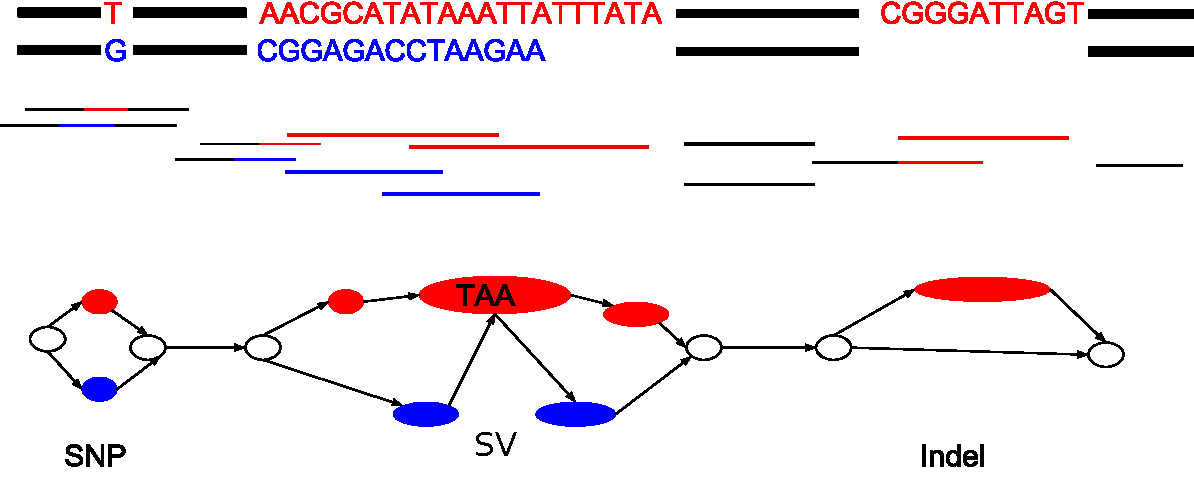
\includegraphics[width=\columnwidth]{ex_sv.pdf}
% \caption{Based on reads (middle) from the two sequences (top), the bubbles in the graph (bottom) show three different heterozygous variations; the first one is an SNV, the second one is an SV, and the third one is an indel. }
% \label{fig:ex_sv}
% \end{figure}

% \begin{figure}[t!]\centering
% 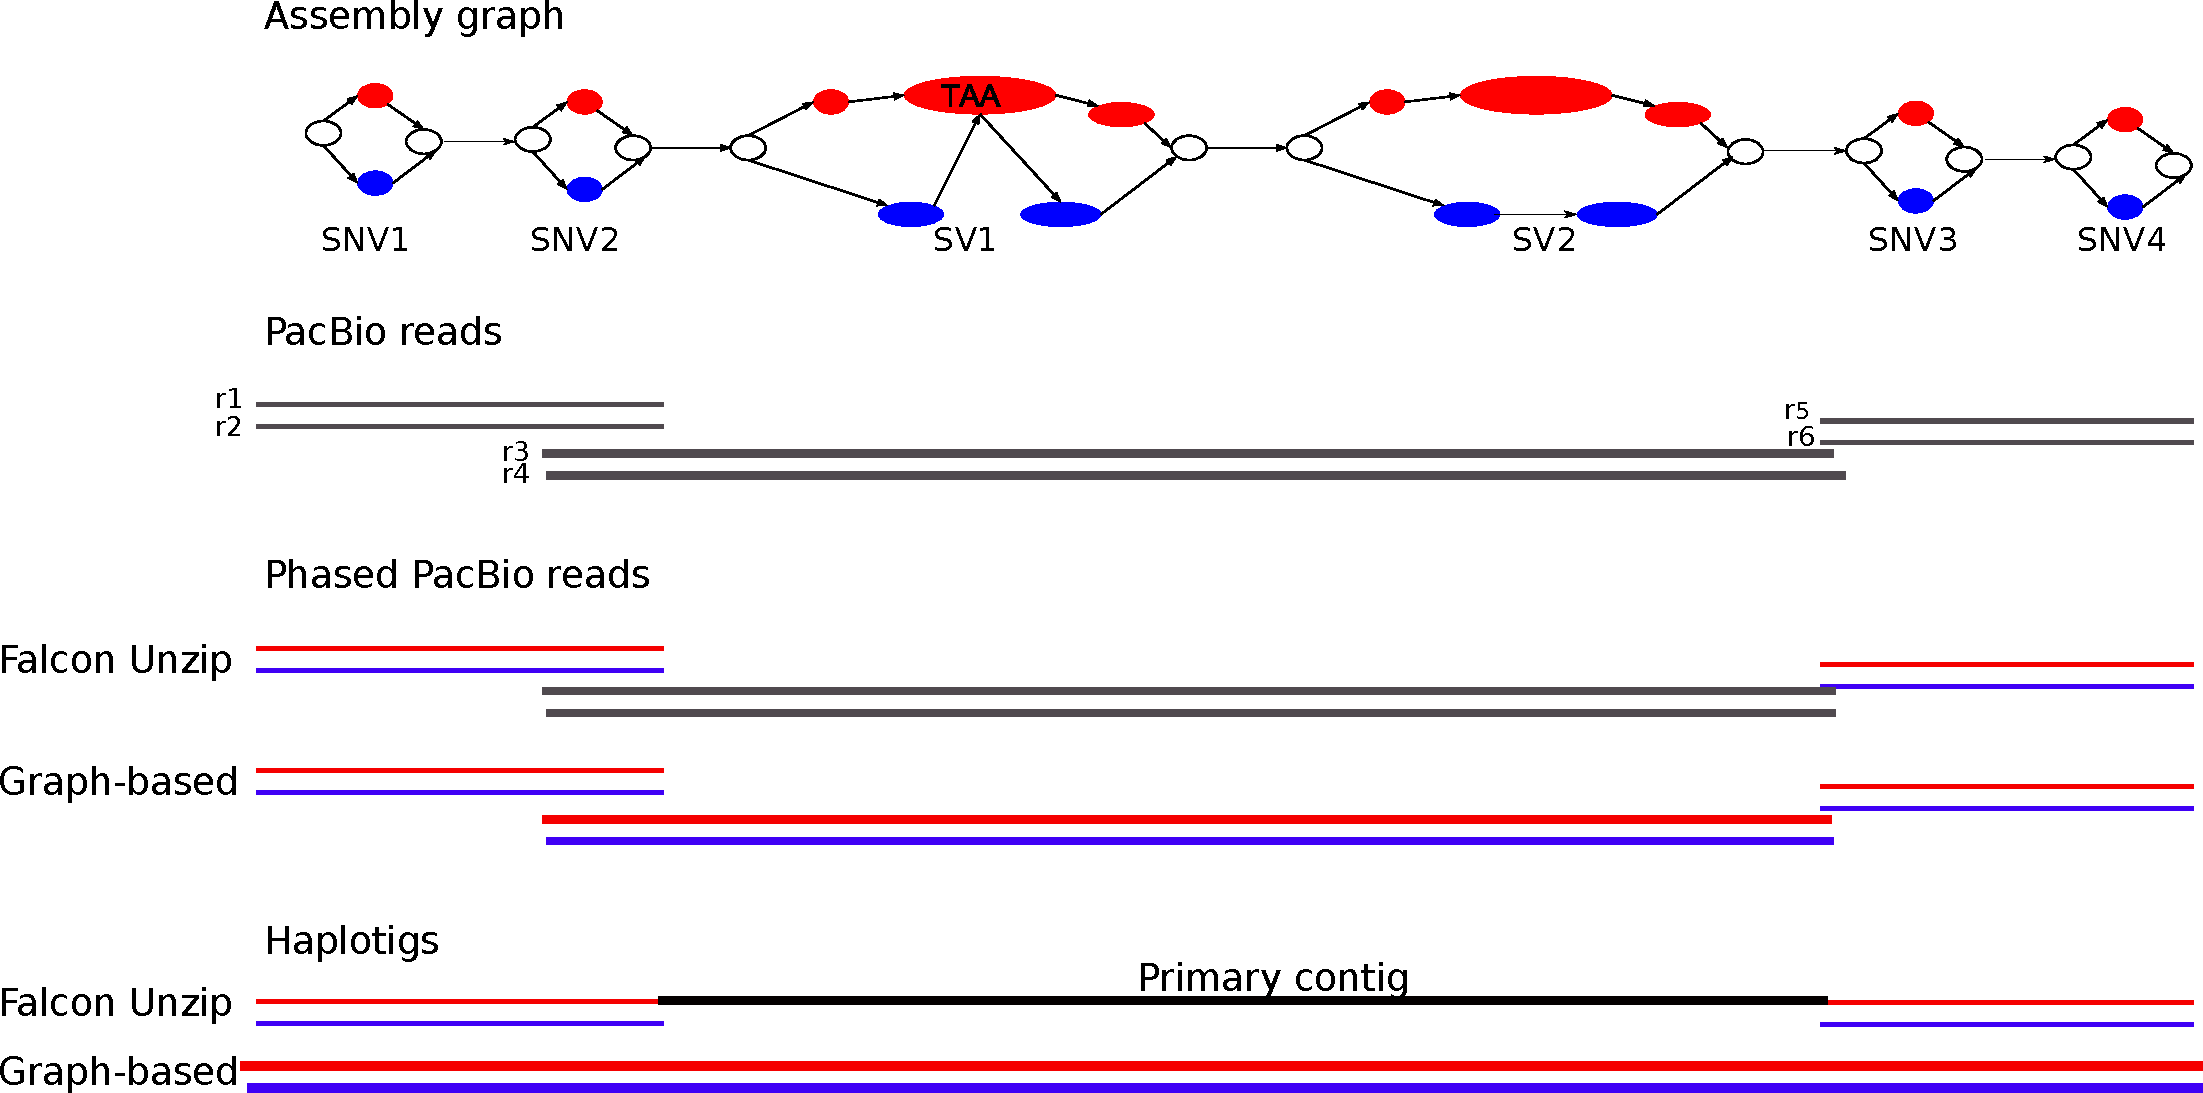
\includegraphics[width=\columnwidth]{ex_graph_approach.pdf}
% \caption{Input: an assembly graph (top) (consisting of four SNVs and two SVs) and the PacBio reads $r_1, r_2, r_3, r_4, r_5, r_6$ (gray). Output: the phased reads (colored in blue and red) and haplotigs (bottom) using Falcon Unzip and our graph-based approach. 
% Our graph-based approach delivers end-to-end haplotigs. Contrarily, Falcon Unzip does not phase the central section, which does not contribute to the total haplotig size.}
% \label{fig:ex_graph_approach}
% \end{figure}
% https://dl.acm.org/citation.cfm?id=322075
% https://www.ncbi.nlm.nih.gov/pmc/articles/PMC5411783/
% http://journals.plos.org/plosone/article?id=10.1371/journal.pone.0019175
\section{Further related work}
The assembly problem was initially formalized as the shortest common super-string problem \citep{maier1978complexity} to generate consensus sequence.
The SCS problem turned out to be NP-hard, thus \cite{tarhio1988greedy} followed the greedy approach to find an approximate solution to solve the assembly problem.
The basic idea of this approach is to combine the two reads that overlap to a maximum extent in terms of length or base quality estimates.
This process is repeated until a predefined minimum quality threshold is reached.

The initial genome assemblers \citep{sutton1995tigr, Green99phrapdocumentation} were based on the greedy strategies and have been used during the Human Genome Project.
Greedy approaches were also explored for datasets generated by second-generation DNA sequencing technologies \citep{warren2006assembling, jeck2007extending}.

The major disadvantage of these greedy approaches is that the shortest common super-string problem neglects an essential feature of complex (e.g.,
vertebrate) genomes: repeats. This has led to the invention of graph-based models for sequence assembly to handle repeats and other complex genomes.
Graph-based models form the basis of most current genome sequence assemblers. 
As introduced in Chapter 1, there are basically two types of graph models such as de Bruijn and OLC-based string graphs.
Over the last few years, a lot of effort has been devoted to improving the graph based assemblers. 

The Edena assembler followed the string graph approach for short-read sequencing data \citep{hernandez2008novo}. To efficiently construct the string graph, several assemblers were developed using the FM index \citep{simpson2010efficient}, 
which led to memory-efficient assemblers for large genomes \citep{li2012exploring, simpson2012efficient}.
Furthermore, several fast string graph construction algorithms were developed \citep{dinh2011memory, gonnella2012readjoiner, ben2014string}.
 
\begin{figure}[t!]\centering
\includegraphics[width=\columnwidth]{{cropped_falcon-unzip}.pdf}
\caption{(a) An initial assembly graph is constructed by FALCON by error-correcting the reads. 
The bubbles are collapsed into a consensus sequence ``primary contig''.
(b) Heterozygous SNPs  are identified and phased, thus haplotype of reads is identified. (c) The phased reads are used to incorporate the haplotype-fused path into the initial assembly graph, thus finally a set of primary contigs and associated haplotigs are generated.
Figure from paper ``Phased diploid genome assembly with single-molecule real-time sequencing''.}
\label{fig:falcon_unzip}
\end{figure}
In the direction of de Bruijn graph, there were also quite a lot of efforts involved.
The ABySS assembler \citep{simpson2009abyss} introduced a representation of
the graph as a hash table of k-mers, with each k-mer storing a byte representing the presence or absence of its eight possible
neighboring k-mers. This representation helped in computational gain by allowing the hash table to be distributed across a cluster
of computers. In recent years, the use of Bloom filters \citep{bloom1970space} has been gaining popularity by representing a set of k-mers.
The Bloom filter was first applied to k-mer counting by \cite{melsted2011efficient}. 
The FM-index data structure \cite{ferragina2000opportunistic}, which was basically designed for mapping reads to the reference genome, was also used for
sequence assembly. 
The FM-index, with slight modifications, has been recently used for representing de Bruijn graphs \citep{bowe2012succinct, rodland2013compact}.
The main point that only a fraction of k-mers need to be directly stored as vertices was observed by \cite{ye2012exploiting}. A similar
technique was used to improve the memory consumption of the popular SOAPdenovo assembler \citep{luo2012soapdenovo2}.

Several algorithms that particularly consider the mate-pair information during assembly have been developed .
 In the works of \citep{butler2008allpaths, bankevich2012spades}, the assembler attempts to enumerate all the paths connecting the endpoints of a mate pair.
The paired de Bruijn graph \citep{medvedev2011paired} approach modifies the de Bruijn graph
structure to implicitly encode the mate-pair information, thereby resolving segments of the graph based on the mate-pair information.
\paragraph{Long-read assemblers}
Although these short-read assemblers can generate consensus sequences to span entire chromosomes, they are very fragmented and lack the finer resolution required to improve contig lengths. 
Instead, the biggest gains in contig lengths stem from single-molecule sequencing, which generates long-read datasets.
These long-read technologies such as PacBio and ONT can generate reads much longer than Illumina. 
More specifically, these reads are long enough to cover the most common repeats in both microbial and vertebrate genomes and can therefore generate highly continuous assemblies. 
Subsequent efforts have been devoted to handling long read lengths and decreasing error rates to generate good quality assemblies.
This includes assembly tools designed specifically for long-read PacBio and Nanopore data: Canu \citep{koren2017canu}, HINGE \citep{kamath2017hinge}, Racon \citep{vaser2017fast}, Falcon \citep{chin2016phased}, and Miniasm \citep{li2016minimap}.

Canu, which is based on Celera Assembler, has been specifically designed for noisy single-molecule sequences.
Canu follows an adaptive overlapping strategy based on tf-idf weighted MinHash \citep{berlin2015assembling} and a sparse assembly graph construction.
It was mainly designed to support long-read data, to be efficient in terms of run-time and coverage requirements, and additionally perform repetition and haplotype separation.
Racon corrects assemblies by finding a consensus sequence between reads and the assembly through the construction of partial order alignment (POA) graphs.
After aligning the reads by a mapper of choice (e.g. Minimap or Graphmap),
Racon segments the sequence and finds the best alignment between a POA graph of the reads and the assembly.
The HGAP (Hierarchical Genome Assembly Process) pipeline
was developed to assemble PacBio-generated data without requiring correction using short-read
data \citep{chin2013nonhybrid}. HGAP is a hierarchical pipeline; it selects the longest PacBio reads to form the basis
of the assembly and error-corrects this subset of reads using the remaining data. The corrected
long reads are then assembled, and a consensus sequence is generated using the complete data
set. This method often generates single-contig assemblies of bacterial genomes.
The FALCON assembler follows the design of the hierarchical genome assembly process (HGAP) but uses more computationally optimized components. It uses string graph algorithm for genome assembly and being best suited for PacBio reads.
It includes several important steps: error correction of raw reads, pre-assembly error correction, overlap filtering, graph construction from overlaps and contig construction from graph.

\paragraph{Hybrid assemblers}
Besides short and long-read assemblers, the hybrid approaches to combine different sequencing datasets provide another avenue for generating accurate, contiguous and complete assemblies. 
The hybrid assemblers, SPAdes by \cite{bankevich2012spades} and ALLPATHS-LG by \cite{gnerre2011high}, are DBG-based, which constructs the base graph using Illumina data and then scaffold the assemblies using longer, less accurate reads such as PacBio. 
Furthermore, SPAdes also supports ONT data as the long read complement to NGS data. 
Recently, \cite{fan2017hysa} demonstrates that the combination of PacBio and Illumina delivers accurate structural variant calls.

\paragraph{Other technologies}
An emerging trend to generate accurate, contiguous and complete assemblies is, to combine cost-effective Illumina sequencing dataset with other sequencing techniques. 
One powerful sequencing technique is chromatin conformation capture via proximity ligation and high-throughput sequencing (Hi-C) \citep{lieberman2009comprehensive}. 
This technique involves in generating a paired-read data type (two reads separated by some distance) but from a distribution of sizes that can span mega bases. 
The main advantage of these data sets is in the scaffolding step to connect contigs, which help in generating chromosome-length scaffolds, and phase haplotypes \citep{burton2013chromosome, selvaraj2013whole}. 
Along the similar lines, \cite{rice2017improved} demonstrates on using in vitro reconstituted chromatin and Illumina sequencing to assemble the American alligator genome. 
Another sequencing technique is the barcoding of short reads to tag groups of ``linked reads'' that all originate from a larger, single molecule of DNA. 
For these synthetic long-read data, \cite{weisenfeld2017direct} introduces a new assembler, Supernova, for the de novo assembly of diploid human genomes. 
Additionally, in the latest version of the ABySS assembler, \cite{jackman2017abyss} explores linked reads and optical mapping for improved scaffolding.
\paragraph{Diploid assemblers}
To date, there is only one diploid assembler, Falcon Unzip. It's pipeline is given in Figure~\ref{fig:falcon_unzip}.
Falcon Unzip first constructs a string graph by using PacBio reads and then collapse the bubbles representing divergent regions between homologous sequences (Fig.~\ref{fig:falcon_unzip}a) to generate sets of ``haplotype-fused contigs'' , also called ``primary contigs''. 
Next, Falcon-Unzip identifies phase of reads using aligned reads over heterozygous SNVs. (Fig.~\ref{fig:falcon_unzip}b). 
The aligned reads provides information on how alleles at heterozygous positions are connected. Based on the aligned reads, Falcon Unzip identifies haplotypes for the genome and phases each read using greedy approach.
Phased reads are then used to assemble haplotigs and primary contigs (Fig.~\ref{fig:falcon_unzip}c) 
that form the final diploid assembly with phased single-nucleotide polymorphisms (SNPs) and structural variants (SVs).
\begin{figure}[t!]\centering
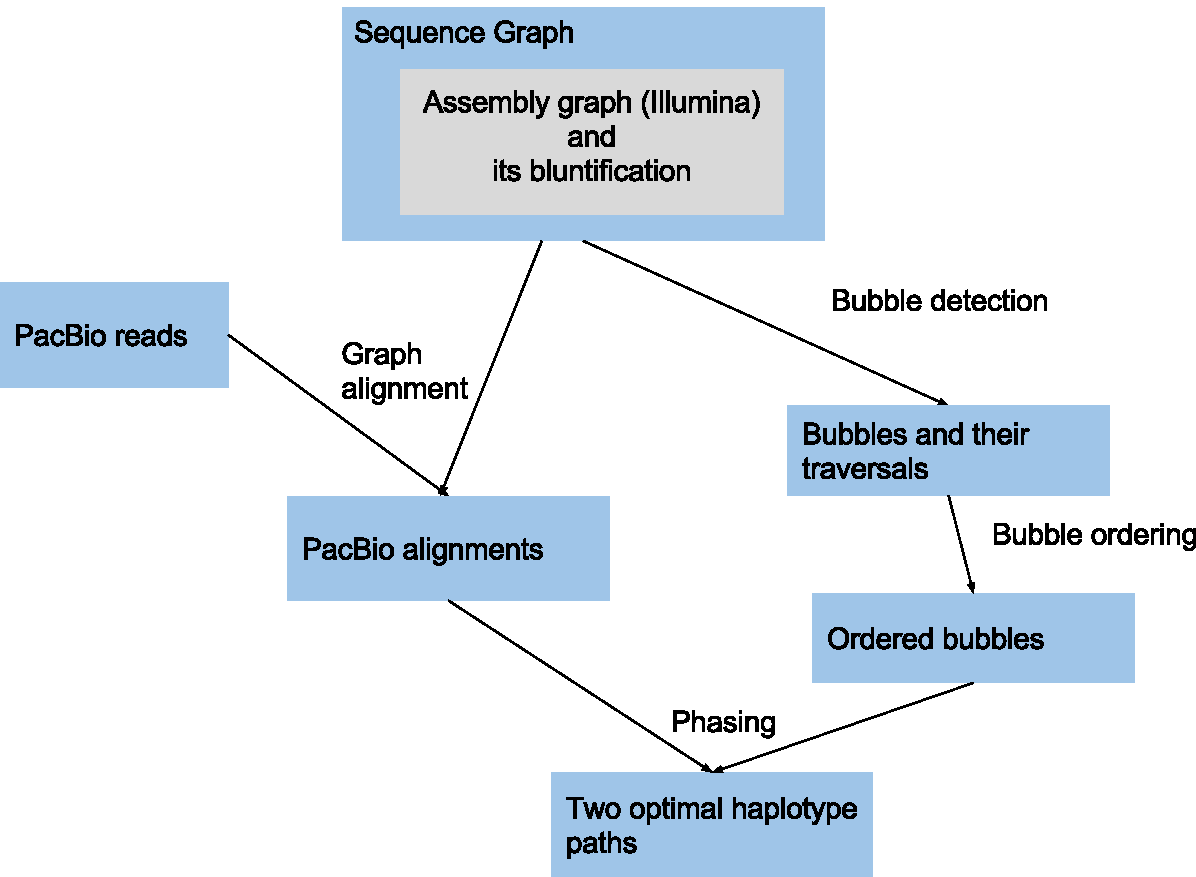
\includegraphics[width=.8\columnwidth]{pipeline.pdf}
\caption{Overview of the diploid assembly pipeline. }
\label{fig:pipeline}
\end{figure}

\textit{Phasing using primary contigs.}
In Falcon Unzip, the reads are aligned to primary contigs and heterozygous SNPs (het-SNPs) are called by considering signal from sequence alignments over these hets.
A simple phasing algorithm is followed to identify phased SNPs using greedy approach. 
Along each contig, the algorithm assigns phasing blocks where ``chained phased SNPs'' can be identified. 
In a contig, the phase to aligned reads to that contig can be assigned unambiguously if read covers sufficient heterozygous SNVs.
Based on the information from primary contig and phased read set, Falcon Unzip assigns a phased tag.
Some reads might not have enough phasing information. For example, if there are not enough het-SNP sites covered by a read, it assigns a special 'un-phased tag' for each un-phased read.
The initial assembly graph is fused using phased reads and the haplotigs are generated in a greedy manner using local conservative approach.
% \todo{maybe add example how haplotigs from haplotype fused assembly graph works?}

\section{Diploid assembly pipeline}
Our assembly workflow uses short read (e.g.\ Illumina) and long read (e.g.\ PacBio) data combinedly, as illustrated in Figure~\ref{fig:pipeline}, and we describe the details of this process in the following.

\subsection{Sequence graph} 
Our first step is to construct a sequence graph using short read data with a low error rate, as provided by the Illumina platform.
% The diploid assembly problem can be modelled using a sequence graph (defined below). We construct the underlying sequence graph using Illumina data.
\begin{definition}[Sequence Graph]
We define a sequence graph $G_s (N_s, E_s)$ as a bidirected graph, consisting of a set of nodes $N_s$ and a set of edges $E_s$.
The nodes $n_i$ are sequences over an alphabet $\mathcal{A} = \{A,C,G,T\}$.
For each node $n_i \in N_s$, its reverse-complement is denoted by $n'_i$.
An edge $e_{i'j}$ connects the nodes $n'_i$ to $n_j$. 
Nodes may be traversed in either the forward or reverse direction, with the sequence being reverse-complemented in the reverse direction. 
% \todo{There was a left/right in the definition at some point. Where did it go (and why)?} \sgnote{Richard and I prefer to write in the language of n and n', it is easier and more mathematical. What do you think? TM: That's ok with me. (Although I disagree that it's more mathematical.)}
\end{definition}

In words, edges represent adjacencies between the sequences of the nodes they connect.
Thus, the graph implicitly encodes longer sequences as the concatenated sequences of the nodes along walks through the graph.

To illustrate this, we consider an example sequence graph $G_s$ in Figure~\ref{fig:wmec}. It consists of a node set $N_s = \{1, 1', 2, 2', 3, 3', \ldots\}$
and an edge set $E_s = \{1 \rightarrow 2', 1 \rightarrow 3' \ldots\}$.

To generate the sequence graph $G_s$, we first employ SPAdes \citep{bankevich2012spades}, which constructs and simplifies a de Bruijn graph, and we subsequently remove the overlaps between the nodes in the resulting graph in a process we call \textit{bluntification}, explained in the Supplement.

\subsection{Bubble detection in sequence graphs} To account for heterozygosity in a diploid genome, we perform bubble detection. The notion of \textit{bubble} we use is closely based on the \textit{ultrabubble} concept as defined by \cite{paten2017superbubbles}. Briefly, bubbles have the following properties:
\begin{itemize}
 \item \textit{2-node-connectivity}. A bubble is bounded by fixed start and end nodes.
 Removing both the start and end nodes disconnects the bubble from the rest of the graph.
 Note that a bubble can be viewed in either orientation.
 If the graph is traversed in one direction, and a bubble is encountered that starts at a node $n_i$  and ends at a node $n'_j$, then that bubble can also be described as the bubble with start node $n_j$ and end node $n'_i$, as it would be encountered when traversing the graph in the opposite direction.
  \item \textit{Directed acyclicity}. A bubble is directed and acyclic.
 \item \textit{Directionality}. All paths through the bubble flow from start to end.
 \item \textit{Minimality}. No vertex in the bubble other than the start node $n_i$ (with proper orientation) forms a pair with the end node $n'_j$ (with proper orientation) that satisfies the above properties. Similarly, no vertex in the bubble other than $n'_j$ forms such a pair with $n_i$.
%  \todo{Reword to avoid ``Only the smallest possible bubble ... is a bubble'' (because larger structures are no bubbles)}
\end{itemize}

A bubble can represent a potential sequencing error or genetic variation within a set of homologous molecules.
We represent bubbles as collections of alternative paths.

\begin{definition}[Path] We define path $a_i$ as a linear ordering of nodes $a_i= n_1, \ldots n_m$. 
% \todo{Why start from a complemented node $n'_1$?}
\label{def:allele-path}
\end{definition}

A bubble is a collection of paths with the same start and end node and can be defined as follows:
\begin{definition}[Bubble]
Formally, a bubble is represented as a collection of allele paths
 $l_k= \{a_1,a_2 \ldots\}$
 where 
 \[a_1=(n_1, n_2, \ldots n_m), a_2=(n_1, n_3 \ldots n_m)\] and so on. 
\end{definition}


For example, Figure~\ref{fig:wmec} shows a set of two bubbles $L=\{l_2, l_1\}$, and the set of allele paths for the
% \todo{TM: did you define ``complex bubble'' already?} 
bubble $l_2$ is $\{a_1, a_2, a_3\}$,
where $a_1 = (6, 7', 8', 11')$, $a_2 = (6, 9', 11')$, $a_3=  (6, 10, 11')$.

\subsection{PacBio alignments} 
For phasing bubbles, we consider long reads from third generation sequence technologies such as PacBio.
We align these long reads to the sequence graph $G_s$ to generate paths through the graph.
We perform graph alignment using a banded version of the algorithm described by \cite{rautiainen2017aligning}, which is a generalization of semi-global alignment to sequence-to-graph alignment\footnote{\url{https://github.com/maickrau/GraphAligner}}.

There are several advantages of aligning PacBio reads to graphs instead of to a reference genome or contigs.
SNPs often occur near larger variants such as insertions and deletions. SNPs are thus often missed in these regions when reads contain large mismatches with respect to the linear sequences they are aligned against. Graph alignment allows the alignment of reads to variants appropriate to each read's phase, and to other types of complex events.

\begin{definition}[Alignment]
We define a set of read alignments as $R=\{r_1, r_2, \ldots, r_j\}$, where each read alignment $r_{j}$ is given by a path of oriented nodes in graph $G_s$, written $r_{j}=(n_1, \ldots, n_m)$.
\end{definition}
For example, in Figure~\ref{fig:wmec}, $R = \{r_1, r_2, r_3, r_4\}$ and the read alignment path $r_1$ can be written as 
$r_1 = (1, 2', 5', 6, 7', 8', 11' ) $


\subsection{Bubble ordering}
The next stage of our algorithm is to obtain an ordering of the bubbles $L=(l_1, l_2, \ldots l_k)$, which we refer to as a \emph{bubble chain}. 
For example, in Figure~\ref{fig:wmec}, $L=(l_1, l_2)$ is a bubble chain.
A general sequence graph $G_s$ is cyclic, due to different types of repeats present in the genome that create both short and long cycles.
Ordering bubbles in such a graph is closely related to resolving repeats, which is a challenging problem.
In this study, we rely on the Canu algorithm \citep{koren2017canu} to provide a bubble ordering by aligning Canu-generated contigs to our sequence graph.
Furthermore, we detect repetitive bubbles---that is, bubbles that would need to be traversed more than once in a final assembly---based on the depth of coverage of aligned PacBio reads, and remove such bubbles.
% \todo{Shilpa, please check these sentence. I reworded them a bit.}
We deem a bubble repetitive if the number of PacBio reads aligned to its starting node is greater than a coverage threshold specified by the user over the genome.
For example, given a 30$\times$ ($=c$) data set and a repeat that occurs 20 ($=r$) times in the genome, then the coverage at the bubble on average is 600 ($=r \cdot c$).

\subsection{Graph-based phasing}
\label{sec:phasing} 
Given a sequence graph $G_s$, ordered bubbles $L$, and PacBio alignments $R$, the goal is to reconstruct two haplotype sequences $\{h_0, h_1\}$, called haplotigs, along each chain of bubbles.
\begin{definition}[Haplotype path]
Formally, a pair of haplotype paths $(h_0, h_1)$ can be defined as two paths through a bubble chain in the sequence graph and denoted as:
\[h_0=(n_s, n_2, \ldots n_e )\]

\[h_1=(n_s, n_3, \ldots n_e )\]

where $h_0$ and $h_1$ may differ at the heterozygous regions defined by bubbles, and $n_s$ and $n_e$ are the start and end of the bubble chain.
% \todo{I'm really confused by these $n'$s. I think we can just use plain $n$s.}
\end{definition}

The two genome sequences can be seen as two walks through the bubbles $L$ in the sequence graph $G_s$ that are consistent with the PacBio alignments $R$.
In maximum likelihood terminology, the goal is to find the most likely haplotype paths given the alignment paths traversing through the bubbles.
For example, in Figure~\ref{fig:wmec}, given bubbles $(l_1, l_2)$ and PacBio alignments $R=\{r_1,r_2,r_3,r_4\}$, the goal is to find two maximum likelihood haplotype paths $\{h_0, h_1\}$ such that each PacBio alignment is assigned to one of the haplotypes. 
% \todo{continue with ``that...'', because you do not just want to find any two paths, but ML ones.}

For a linear chain of bubbles $L$, the task of finding these two haplotype paths is equivalent to picking one allele path per haplotype for each bubble.
% We generate an association between bubbles $L$ and aligned PacBio reads $R$ in the sequence graph $G_s$ in order to encode alignment paths in the form of an allele path in bubbles.
To this end, we note that an alignment path $r_j$ for a given read can be viewed as a sequence of allele paths traversed in consecutive bubbles. 
% stores the information about the allele path $a_i$ in a bubble $l_k$ that the read $r_j$ is aligned.
We represent this association of reads to allele paths in the form of a \emph{bubble matrix} $\mathcal{F}\in\{0,1, \ldots m, -\}^{|R|\times |L|}$, where $|R|$ is the number of reads, $|L|$ is the number of bubbles along a chromosome, and $m = \max_k|l_k|$ is the maximum number of  paths (or alleles) in any bubble $l_k\in L$.
% Please note that the different paths in a bubble corresponds to possible alleles at a genetic variant.
The entry $\mathcal{F}(j,k) \in \{0, 1, \ldots m, -\}$ represents the allele path index in bubble $l_k$ that read $r_j$ is aligned to, where a value of ``$-$'' indicates that the read does not cover the bubble.
% For example, in Figure~\ref{fig:wmec}, the read alignment path $r_1$ traverses an allele path $a_1$ in a bubble $l_1$ and $a_1$ in $l_2$. \todo{TM: The allele paths are not shown in that figure, right? Can we add them?}
In Figure~\ref{fig:wmec}, note that the read alignment path $r_4$ does not cover all the nodes in any of the allele paths in $l_2$ and hence we set the corresponding value $\mathcal{F}(4,2)$ to ``$-$''.
As a result, this read covers only one bubble, which renders it uninformative for phasing, and we do not consider it further.
The remaining phasing-informative reads in Figure~\ref{fig:wmec} are represented as:

\begin{equation}\label{eq:bubble_matrix}
  \mathcal{F}  = \kbordermatrix{
     & l_{1}       & l_{2}  \\
    r_{1}       & 0 & 0 \\
    r_{2}       & 2 & 2 \\
    r_{3}       & 1 & 2 \\
  }
\end{equation}

Corresponding to $\mathcal{F}$, we have a weight matrix $\mathcal{W}\in W^{|R|\times |L|\times m}$. %, where $|R|$ is the number of reads, $|L|$ is the number of bubbles and $m$ is the maximum number of alleles in a bubble $l_k$.
Each entry in $\mathcal{W}(j,k)$ is a tuple storing a weight for each allele, which can for instance reflect ``phred-scaled'' (i.e. $-10\log(p)$) probabilities that the read supports a given allele.
The weight of ``0'' at the $i^\text{th}$ entry in the tuple $\mathcal{W}(j,k)$ encodes that the read $r_j$ is aligned to allele path index $i$ in bubble $l_k$.
The remaining non-zero values in tuple $\mathcal{W}(j,k)$ store the confidence scores of switching the aligned read $r_j$ to other alleles in bubble $l_k$.

For example, the corresponding weight matrix $\mathcal{W}(j,k)$ for $\mathcal{F}$~\eqref{eq:bubble_matrix} is given by:
\begin{equation}\label{eq:weight_matrix}
  \mathcal{W}  = \kbordermatrix{
     & l_{1}       & l_{2}  \\
    r_{1}       & [0,q_1,q_2] &  [0,q_3,q_4]\\
    r_2 & [q_9,q_8,0] & [q_{11},q_5,0] \\
    r_3 & [q_{10},0,q_7] & [q_5,q_6,0] \\
  }
\end{equation}
where the entry $\mathcal{W}(1,1)$ value $[0,q_1,q_2]$ means that the read $r_0$ is aligned to allele $a_0$ at bubble $l_1$.
Additionally, the cost of flipping it to other alleles is $q_1$ for $a_1$ and $q_2$ for $a_2$.
% \todo{We should use different $q$s for each entry.}

We are now ready to present the problem formulation.
The main insight is that solving phasing for bubble chains is similar to solving the phasing problem for multi-allelic SNVs in reference-based haplotype reconstruction.
Therefore, we build on the previous formulation of the Minimum Error Correction (MEC) problem \citep{Lancia2001} and its weighted version (wMEC) \citep{lippert2002algorithmic,Patterson2015} and further adapt it to work on a subgraph consisting of a chain of bubbles, defining the \emph{Minimum Error Correction for graphs} (gMEC) problem.

\begin{figure}[t!]\centering
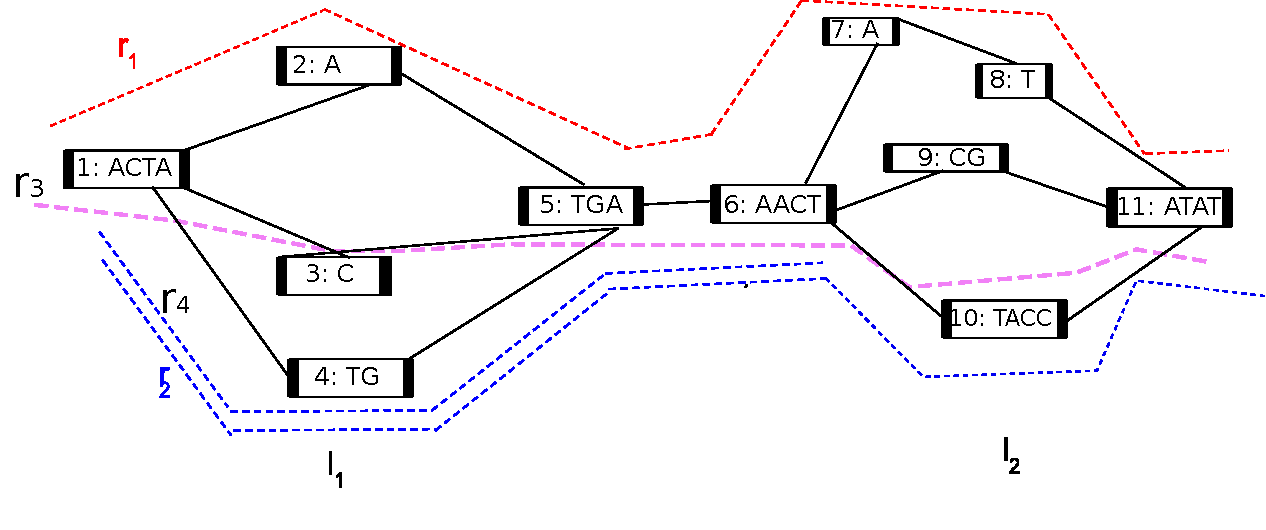
\includegraphics[width=\columnwidth]{wmecfig.pdf}
\caption{For a subgraph of $G_s$, the example shows two bubbles $l_1$ and $l_2$, and their corresponding alleles. Reads $r_1,r_2,r_3,r_4$ traverse the bubbles.}
\label{fig:wmec}
\end{figure}

% \begin{definition}[Distance] 
% The quality of a solution relies on the measure $d(r_1,r_2)$ based on the Hamming distance between any two rows $r_1,r_2$. Formally,
% \[d(p_1,p_2):=\sum_{k=1}^{|L|} \big|\big\{k\,\big|\,r_1(k)\neq -\ \wedge\ r_2(k)\neq -\ \wedge\ r_1(k)\neq r_2(k)\big\}\big|.\]
% \end{definition}
% 
% \begin{definition}[Feasibility]
% A feasible solution to a bubble matrix $\mathcal{F}\in\{a_0, a_1 \ldots a_m, -\}^{|R|\times |L|}$ is a pair of haplotypes $h^0,h^1\in\{a_0, a_1, \ldots a_m\}^M$ such that 
% \[d(h_0,h_1):=\sum_{j=1}^{|R|} \min\{ d(\mathcal{F}(j), h_0), d(\mathcal{F}(j), h_1)\} \]
% and there exists a bi-partition of rows (i.\,e., reads) into two sets such that all pairwise distances of two rows within the same set are zero.
% \end{definition}

\begin{problem}[wMEC for bubble chains (gMEC)]\label{prob:gMEC}
Assume we are given a bubble chain $L=(l_1,\ldots,l_{|L|})$ and a set $R$ of aligned reads $r_j$ that pass through these bubbles, with $\mathcal{F}(j,k)$ indicating the index of the allele in bubble $l_k$ that the alignment of read $r_j$ passes through, or ``$-$'' if it does not pass through $l_k$, and that $\mathcal{W}(j,k,i)$ is the cost of flipping $\mathcal{F}(j,k)$ to new value $i$.  
We want to find two paths through $L$, each of which consists of a sequence of allele indices specifying which allele the path takes in each bubble $l_k$, and then to flip entries of $\mathcal{F}$ such that each row is equal to one of the paths for all non-dash entries while the incurred costs are minimized.
\end{problem}
% For simplicity, we represent the $i^{th}$ element of tuple $\mathcal{W}(j,k)$ as $\mathcal{W}(j,k,i)$.
Note that the wMEC problem constitutes a special case of gMEC, where the input graph is a chain of bi-allelic bubbles.
% In its linear counterpart, wMEC with each entry in $\mathcal{F}(j,k) \in \{0,1\}$ works for bi-allelic cases.
Next, we describe how to solve gMEC via dynamic programming (DP).

In the WhatsHap algorithm \citep{Patterson2015}, wMEC is solved in an exact manner for bi-allelic variants using a dynamic programming approach.
It runs in $\mathcal{O}(2^c\cdot |L|)$ time, where $|L|$ is the number of variants to be phased and $c$ is the maximum physical coverage.
The basic idea is to proceed column-wise from left to right over a set of active reads.
Each read remains active from its first non-dash position to its last non-dash position in $\mathcal{F}$.
In column $k$, we denote the set of active reads as $A(k)$, particularly, $c=\max_{k}\{|A(k)|\}$.
The algorithm now considers all \emph{bipartitions} of $A(k)$, that is, all pairs $B=(P,Q)$ of disjoint sets $P$ and $Q$ such that $P\cup Q=A(k)$.
We fill a DP table column wise and for each column $k$ of $\mathcal{F}$, we fill a DP table column $C(k,\cdot)$ with $2^\abs{A(k)}$ entries corresponding to these bipartitions of $A(k)$.
Each entry $C(k,B)$ is equal to the cost of solving wMEC on the partial matrix consisting of columns $1$ to $k$ of $\mathcal{F}$ such that the bipartition of the full read set $A(1)\cup\ldots\cup A(k)$ \emph{extends} $B$ according to the below definition.
\begin{definition}[Bipartition extension]
For a given set $A$ and a subset $A'\subset A$, a bipartition $B=(P,Q)$ of $A$ is said to \emph{extend} a bipartition $B'=(P',Q')$ of $A'$ if $P'\subset P$ and $Q'\subset Q$.
\end{definition}

Once all entries of the DP table have been computed, the minimum of the last column $\min_B\{C(|L|,B)\}$ indicates the optimal wMEC cost and the optimal bipartition can be obtained by backtracing.
We refer the reader to \cite{Patterson2015} for a more detailed explanation of this algorithm.

\textit{Solving gMEC for bubble chains}. The basic idea is to now extend the dynamic program to consider all possible path-pairs through each bubble. 
In the bi-allelic case, we have only two paths in every bubble and, therefore, there is only one pair of distinct paths.
In the multi-allelic case, we consider all possible path pairs in each bubble.
The goal is to find an optimal pair of paths from the sequence graph $G_s$.
% \todo{what does ``simplified version'' refer to? After repeat removal?} 
Analogously to the WhatsHap algorithm for wMEC, we proceed from left to right using dynamic programming.  
% Assuming we have completed the process up to bubble $l_k$, at bubble $l_{k+1}$ we consider each possible bipartition of all the reads crossing that bubble into two groups.\todo{TM: unclear wording}
% For each bipartition, we find the best pair of alleles and the best assignment at $l_k$.\todo{Can we be more precise here and mention costs in this column vs.\ costs from previous columns?}
% We continue this way until the last bubble $|L|$ and then backtrace to get the two optimal paths.

To explain the dynamic programming algorithm that we use, consider a toy example with the weight matrix~\eqref{eq:weight_matrix}:
\begin{equation}\label{eq:weight_matrix1}
  \mathcal{W}  = \kbordermatrix{
     & l_{1}       & l_{2}  \\
    r_{1}       & [0,10,5] &  [0,5,8]\\
    r_2 & [7,6,0] & [5,2,0] \\
    r_3 & [2,0,4] & [4,3,0] \\
  }
\end{equation}

\textit{DP cell initialization}. Along similar lines as \cite{Patterson2015}, we first compute the local cost incurred by bipartition $B= (R,S)$ in column $k$, denoted $\Delta_C(k,B)$, and later combine it with the corresponding costs incurred in previous columns.
% We write $\mathcal{S}(k,B)$ to denote this set of sets of reads induced by bipartition $B$ in column $k$.
The cost $W_{k,R}^i$ of flipping all entries in a read set $R$ to an allele index $i\in\{0,1,\ldots |l_k|\}$ is given by 
\[W_{k,R}^i = \sum_{j\in R}\iverl \mathcal{F}(j,k)\neq i\iverr\cdot\mathcal{W}(j,k,i),\]
In the same manner, we can compute costs $W_{k,S}^i$ for read set $S$ to an allele index $i$.

To compute the cost incurred by a bipartition in a particular column $k$, we minimize over all possible pairs of alleles in bubble $l_k$.
There are ${|l_k| \choose 2}$ such pairs.
So given the corresponding column vectors $\mathcal{F}(k)$ and $\mathcal{W}(k)$ of the bubble matrix and of the weight matrix, respectively, and the bipartition $B=(R,S)$ of active reads $A(k)$, the cost $\Delta_C(k,B)$ is computed by minimizing over all pairs of alleles
$A = \{(x,y) \in l_k \times l_k | x \ne y, x\textless y\}$:
\begin{equation}\label{eq:dp-cell}
  \Delta_C(k,B)= \min_{(p_0,p_1)\in {A}}\left\{\min\{W_{k,S}^{p_0} + W_{k,R}^{p_1}, W_{k,S}^{p_1} + W_{k,R}^{p_0}\}\right\},
\end{equation}
where the outer minimization considers all allele pairs and the inner minimization considers the two possibilities of assigning those two alleles to the two haplotypes.

   

% \begin{algorithm}
%     \caption{\label{alg:dp-cell}\textsc{DP CELL INITIALIZATION}}
%     \SetKwInOut{Input}{Input}
%     \SetKwInOut{Output}{Output}
%     \Input{The column vectors of the bubble matrix $\mathcal{F}(k)$ and a weight matrix $\mathcal{W}(k)$ of the bubble $k$, and the bipartition $S$ of active reads $R (k)$}
%     \Output{$\Delta_C(k,B)$}
%     All allele-pairs set $A = \{(x,y) \in l_k \times l_k | x \ne y, x\textless y\}$ from bubble $l_k = \{a_1, a_2, \ldots a_m\}$
%     \[\Delta_C(k,B)= \min_{i\in {A}^{\mathcal{S}(k,B)}}\left\{\sum_{S\in\mathcal{S}(k,B)}W_{k,S}^{i}\right\},\]
%     
% \end{algorithm}

\textit{DP column initialization}. 
We initialize the first DP column by setting $C(1,B):=\Delta_C(1,B)$ for all possible bipartitions $B$.
We enumerate all bipartitions in Gray code order, as done previously in \cite{Patterson2015}.
This ensures that only one read is moved from one set to another in each step, facilitating constant time updates of the values $W_{k,S}^i$.

For a variant matrix~\eqref{eq:bubble_matrix} and its corresponding weight matrix~\eqref{eq:weight_matrix1}, the DP column cell for bipartition $B=(R,S)$ is given by
\[\Delta_C(k,(R,S))= \min\big\{W^0_{k,R} + W^1_{k,S}, W^1_{k,R} + W^2_{k,S}, \]
\[W^0_{k,R} + W^2_{k,S}, W^1_{k,R} + W^0_{k,S},\]
\[W^2_{k,R} + W^1_{k,S}, W^2_{k,R} + W^0_{k,S} \big\}\]
Now, plugging values from~\eqref{eq:weight_matrix1} into the above equation for different bipartitions, $\Delta_C(1,.)$ can be filled as follows:
\[
\begin{split}
\Delta_C(1,& (\{r_1,r_2,r_3\},\emptyset)) =\\ & min\{9+0, 16+0, 9+0,16+0, 9+0, 9+0\} = 9 
\end{split}
\]
% \[C(1, (\{r_1,r_2\},\{r_3\})) = \min\{7+2, 16+0, 5+4, 7+0, 16+4, 7+4\} = 7\]
Similarly, we can compute $\Delta_C(1,.)$ for other bipartitions $(\{r_1,r_2\},\{r_3\}),$\\
$(\{r_1,r_3\},\{r_2\}), (\emptyset,\{r_1,r_2,r_3\}), (\{r_3\},\{r_1,r_2\}), (\{r_2\},\{r_1,r_3\})$.

\begin{algorithm}
    \caption{\label{alg:dp-column}\textsc{DP COLUMN INITIALIZATION}}
    \SetKwInOut{Input}{Input}
    \SetKwInOut{Output}{Output}
    \Input{Set $A(1)$ of reads covering bubble $l_1$.}
    \Output{$C(1,.)$}
    \For{ all bipartitions $B$ of column $k$}{
	Compute $\Delta_C(k,B)$ using Equation~\ref{eq:dp-cell} and store in $C(1,B)$.	
    }
\end{algorithm}
Due to the use of the Gray code order, we can perform this operation for one DP column in $\mathcal{O}( {|l_k| \choose 2} \cdot 2^{|A(k)|})$ time.

\textit{DP column recurrence}.
Note that $C(k,B)$ is the cost of an optimal solution of Problem~\ref{prob:gMEC} for input matrices restricted to the first $k$ columns under the additional constraint that the solution's bipartition of the full read set extends $B$.
Since column $k$ lists all bipartitions, the optimal solution to the input matrix consisting of the first $k$ columns would be given by the minimum in that column.
To compute entries in column $C(k+1,\cdot)$, we add up local costs incurred in column $k+1$ and costs from the previous column (see Algorithm~\ref{alg:dp-table}).
To adhere to the semantics of $C(k+1,B)$ described above, only entries in column $k$ whose bipartitions are \emph{compatible} with $B$ are to be considered as possible ``predecessors'' of $C(k+1, B)$.

\begin{definition}[Bipartition compatibility]
For bipartitions $B = (P, Q)$ of $A$ and $B' = (P', Q')$ of $A'$, $B$ and $B'$ are \emph{compatible} if $P \cap A \cap A' = P' \cap A \cap A'$ and $Q \cap A \cap A' = Q' \cap A \cap A'$, denoted by $B \simeq B'$
\end{definition}

For example, consider the second column from~\eqref{eq:bubble_matrix} and~\eqref{eq:weight_matrix1}. Let us compute $C(2,.)$ for different bipartitions using recurrence in Algorithm~\ref{alg:dp-table}:
\[C(2, (\{r_1,r_2,r_3\},\emptyset)) = \min\{9+0, 10+0, 9+0,10+0, 8+0, 8+0\} \]
\[ + \min\{C(1, (\{r_1,r_2,r_3\},\emptyset)\} = 8+9 = 17 \]

To fill DP column $C(2,.)$, we can analogously compute this for the remaining bipartitions $(\{r_1,r_2\},\{r_3\})$,
$(\{r_1,r_3\},\{r_2\})$, $(\emptyset,\{r_1,r_2,r_3\})$, $(\{r_3\},\{r_1,r_2\})$, and $(\{r_2\},\{r_1,r_3\})$.

\begin{algorithm}
    \caption{\label{alg:dp-table}\textsc{DP TABLE}}
    \SetKwInOut{Input}{Input}
    \SetKwInOut{Output}{Output}
    \Input{$C(1,.)$ for all bipartitions of bubble $k$.}
    \Output{$C(k,.)$ for all the columns $k$ up to the last column $|L|$}
    \For{ all columns $k \in \{2 \ldots |L|\}$}{
        \For{ all bipartitions $B \in \mathcal{B}(A(k))$}{
            Compute $\Delta_C(k,B)$ using Equation~\ref{eq:dp-cell}. \\
            Combine it with cost from column $k-1$ to obtain cost for column $k$:
            \[C(k,B)= \Delta_C(k,B) + \min_{\substack{B'\in\mathcal{B}(A(k-1)):B\simeq B'}}C(k-1,B')\]
        }
        where $\mathcal{B}\big(A(k)\big)$ denotes the set of all bipartitions of $A(k)$.
    }
\end{algorithm}

\textit{Backtracing}. We can backtrace from the last column $C(|L|, \cdot)$ to compute an optimal bipartition $B=(R,S)$ of all input reads.
Given this bipartition, we obtain minimum-cost haplotypes as follows:
Let $B_k=(R_k,S_k)$ with $R_k=R\cap A(k)$ and $S_k=S\cap A(k)$ be the induced bipartition in column $k$.
We then set
\begin{equation}\label{eqn:haplo_c1}
h_0(k)= a_i \quad \text{with } i:=\argmin_{i'\in \{0,1, \ldots |l_k|\}} W_{k,{R_k}}^{i'}, \nonumber
\end{equation}
\begin{equation}\label{eqn:haplo_c2}
h_1(k)= a_j \quad \text{with } j:=\argmin_{j'\in \{0,1, \ldots |l_k|\}} W_{k,{S_k}}^{j'}, \nonumber
\end{equation}
where $a_i$ and $a_j$ refer to the corresponding allele paths of bubble $k$ (see Definition~\ref{def:allele-path}).
% The full length haplotypes $(h_0, h_1)$ are then obtained by concatenating the bubble paths $\big(h_0(k), h_1(k)\big)$ over all bubbles.

\textit{Time complexity}. 
% As in the previous WhatsHap algorithm \citep{Patterson2015}, we performed algorithm engineering to save the phase information from two consecutive bubbles.
Computing one DP column takes $\mathcal{O}( {m \choose 2} \cdot 2^{|A(k)|})$ time, and the total running time is $\mathcal{O}( {m \choose 2} \cdot 2^{|A(k)|} \cdot |L|)$ for $|L|$ bubbles, where $m$ is the maximum number of alleles in any bubble from $L$. 
Running time is independent of read-length and, therefore, the algorithm is suitable for the increased read lengths available from upcoming sequencing technologies.

\subsection{Generation of final assemblies}
To generate final assemblies, for every connected component in the base sequence graph $G_s$, we traverse along the haplotype paths $(h_0,h_1)$ running through that component. For the nodes in each path, we concatenate together the nodes' sequences from the base sequence graph $G_s$ (in either in their forward or reverse-complement orientations, as specified by the path) in order to generate the final haplotig sequences.

\section{Datasets and experimental setup}
To evaluate the performance of our method, we consider the real data available from two haploid yeast strains SK1 and Y12 \citep{yue2017contrasting}, which we combine to generate a pseudo-diploid yeast.
Both the SK1 and Y12 yeast strains are deeply sequenced using Illumina and PacBio sequencing.
The Illumina dataset is sequenced to an average coverage of 469$\times$ with 151\,bp paired end reads. We randomly downsample the dataset to a lower average coverage of 50$\times$.
The PacBio data is sequenced to an average coverage of 334$\times$ with an average read length of 4510\,bp. 
For coverage analysis, we randomly downsample the PacBio reads to obtain datasets of different coverages $10\times$, $20\times$ and $30\times$ with their average read-lengths of 4482, 4501 and 4516\,bp respectively.

\subsection{Pipeline implementation}
\textit{Sequence graph}.
The first step in our pipeline is to perform error correction on the Illumina data by using BFC \citep{li2015bfc}, which, in our experience, retains heterozygosities well for diploid genomes.
BFC is used with default parameters and provided with a genome size of 12.16\,Mbp.
The second step is to generate a sequence graph that includes heterozygosity information.
To construct such a graph, we first construct the assembly graph by using a modified version of SPAdes v3.10.1 \citep{bankevich2012spades}.
We modify the original SPAdes to skip the bubble removal step and retain the heterozygosity information in the graph, and run it with default parameters plus the \texttt{{-}{-}only-assembler} option.
It uses the short Illumina reads to generate a De~Bruijn-based assembly graph without any error correction.
We then convert the assembly graph to a bluntified sequence graph using VG \citep{garrison2017sequence}.
After graph simplification, the resulting sequence graph has 158,567 nodes and 190,767 edges.

\textit{Bubble detection}. In the next stage, we use VG's snarl decomposition algorithm \citep{paten2017superbubbles} to detect the regions of heterozygosity, or \textit{snarls}, in the sequence graph. This results in 29,071 bubbles.
% and 58,183 total alleles of bubbles. 
% \todo{So there must be bubbles with only one allele since $29095\cdot 2= 58190$. How many multi-allelic bubbles are there?}.

\textit{PacBio Alignments}. After bubble detection, we align different coverage levels (10$\times$, 20$\times$ and 30$\times$) of long read PacBio data to the generated sequence graph using GraphAligner\footnote{\url{https://github.com/maickrau/GraphAligner}}.
% For efficient alignment of PacBio reads, we use a seed-based approach.
This resulted in 21,868, 43,459 and 73,129 PacBio alignments for input coverages of $10\times$, $20\times$ and $30\times$, respectively.

\textit{Bubble ordering}. To obtain an ordering of bubbles, we perform \textit{de novo} assembly using Canu v1.5 \citep{koren2017canu} on each PacBio dataset.
As suggested by \cite{giordano2017novo}, we use Canu v1.5 with the following parameter values: \texttt{corMhapSensitivity=high,} \texttt{corMinCoverage=2,} \texttt{correctedErrorRate=0.10,}\\
\texttt{minOverlapLength=499,} \texttt{corMaxEvidenceErate=0.3}.
Next, we align these Canu contigs to the sequence graph to obtain the bubble ordering, which we define as the sequence of bubbles encountered by each aligned contig.
Note that we use Canu solely for bubble ordering.
In this paper, we restrict ourselves to phasing bubbles only in unique, non-repetitive regions.
We detect repetitive bubbles based on the coverage depth of the PacBio alignments and remove them from downstream analyses.
The coverage depth threshold used is 1.67 times the average coverage.
This results in 148, 80, and 71 bubble chains, and 26,576, 27,556 and 27,741 bubbles, at coverages of $10\times$, $20\times$, and $30\times$ respectively.

% \todo{What is the definition of ``ordered bubble''? How many bubble chains and how many bubbles per chain on average?} 
\begin{figure}[t!]\centering
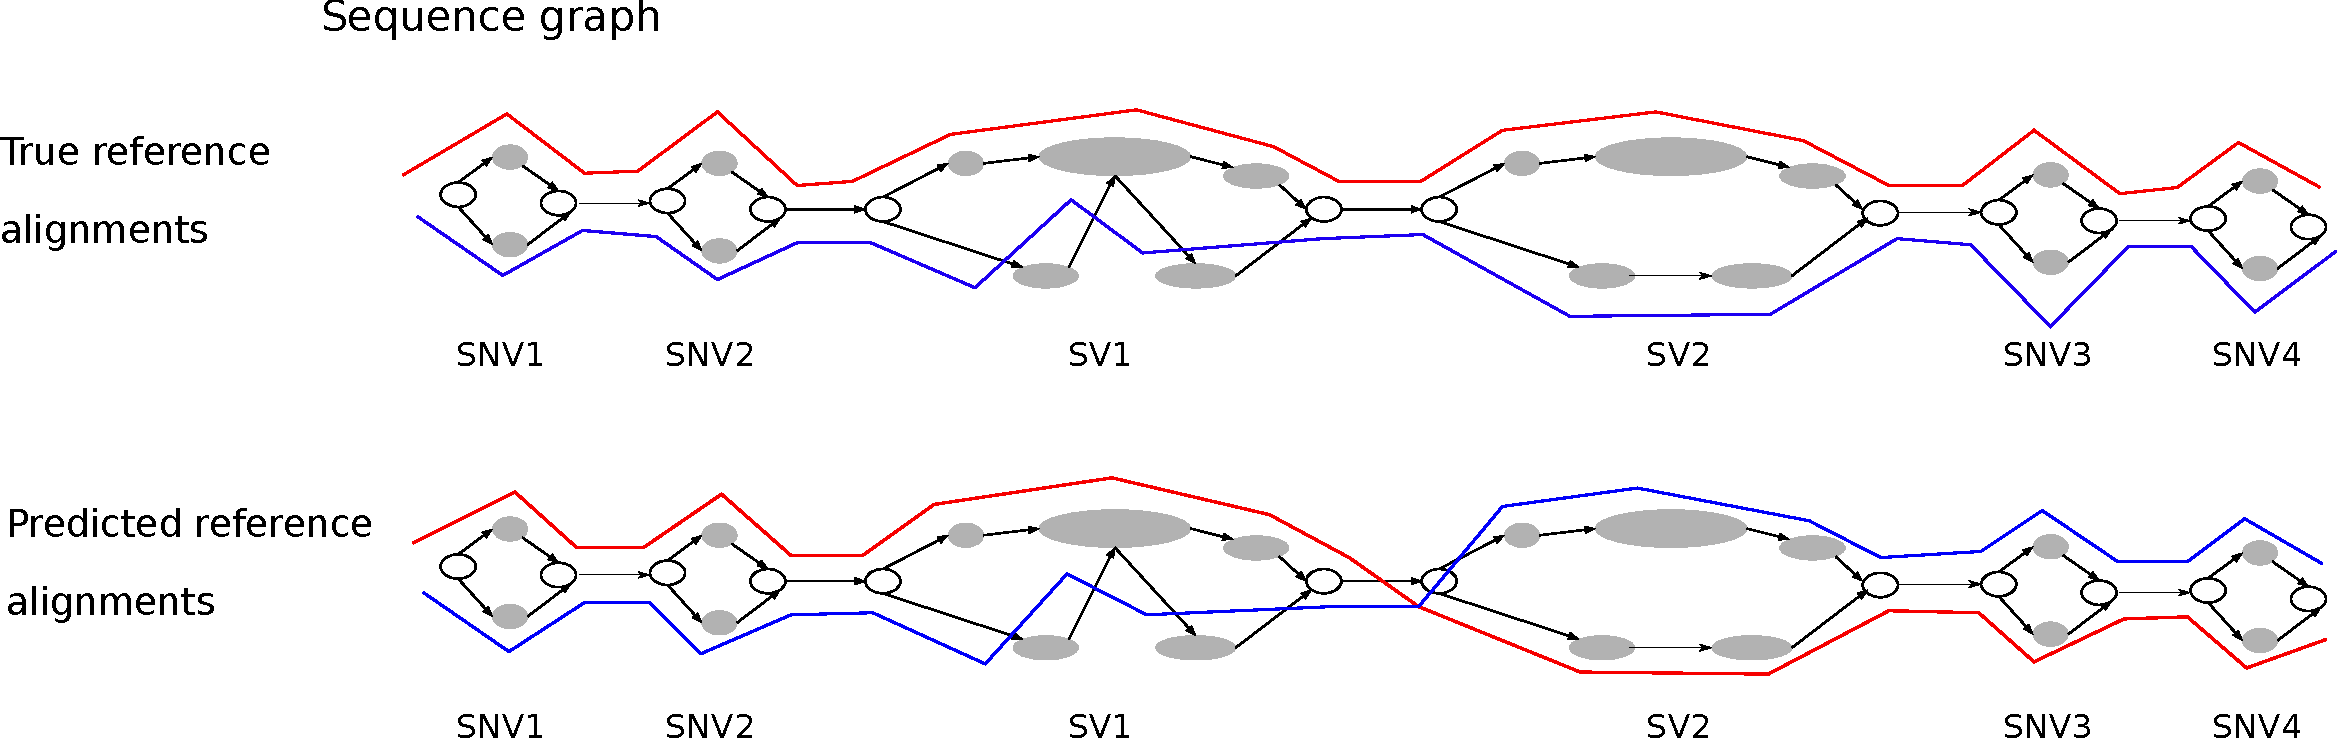
\includegraphics[width=\columnwidth]{evaluation.pdf}
\caption{For a subgraph of $G_s$, this example shows the true (top) and predicted (bottom) versions of two haplotype alignments (red and blue) through a series of bubbles. When comparing the correspondingly-colored lines between the two versions, we see one switch between SV1 and SV2: the prediction contains one switch error. 
Six bubbles have been phased, for a total of five phase connections between consecutive bubbles. Therefore, the phasing error rate is 1/5.}
\label{fig:evaluation}
\end{figure}
\textit{Graph-based phasing}. For each of the coverage conditions, we take as input the ordered bubbles, the long-read PacBio alignments and the sequence graph, and solve the gMEC problem by assuming constant weights in the weight matrix $\mathcal{W}$.
The optimal bipartition is computed via backtracing and the final haplotigs are generated by concatenating the node labels of the two optimal paths.
These steps have been implemented in our WhatsHap software as a subcommand \texttt{phasegraph}\footnote{Presently this functionality resides in the \texttt{MAV} branch, which will be merged to the \texttt{master} branch in the near future and will be part of future WhatsHap releases.}.
\subsection{Running Falcon Unzip}
The main goal of this study is to measure the performance of phasing using a graph based approach, 
and, in particular, the quality of haplotypes at heterozygous sites achievable by using this method with low coverage PacBio data.
Therefore, we compared our graph-based approach to the state-of-the-art contig based phasing method Falcon Unzip, which also generates diploid assemblies.

The Falcon Unzip \citep{chin2016phased} algorithm first constructs a string graph composed of ``haploid consensus'' contigs, with bubbles representing structural variant sites between homologous loci. 
Sequenced reads are then phased and separated for each haplotype on the basis of heterozygous positions. 
Phased reads are finally used to assemble the backbone sequence (primary contigs) and the alternative haplotype sequences (haplotigs). 
The combination of primary contigs and haplotigs constitutes the final diploid assembly, which includes phasing information dividing single-nucleotide polymorphisms and structural variants between the two haplotypes.

We ran Falcon Unzip using the parameters given in the official parameter guide\footnote{http://pb-falcon.readthedocs.io/en/latest/parameters.html}.
We tried to run Falcon Unzip for lower coverages of 10$\times$ and 20$\times$, but it did not generate output in these cases (and we assume it is not designed for such low coverages).
Therefore, we only ran Falcon Unzip for 20$\times$ PacBio coverage.
Primary contigs and haplotigs were polished using the Quiver algorithm and corrected for SNPs and indels using Illumina data via Pilon, with the parameters ``\texttt{{-}{-}diploid}'' and ``\texttt{{-}{-}fix all}'' \citep{walker2014pilon}.
% To compare the Falcon Unzip haplotigs to the true references, we align the haplotigs produced by Falcon Unzip to our sequence graph and then 
% compared these aligned haplotigs to the true reference alignments through the bubbles.

\subsection{Assembly performance assessment}
To evaluate the accuracy of the predicted haplotypes, we align reference assemblies of the two yeast strains SK1 and Y12 \citep{yue2017contrasting} to the sequence graph.
% In doing so, first, we obtain the true references based on previously generated assemblies of two yeast strains SK1 and Y12 using high coverage PacBio data \citep{yue2017contrasting} and, second, we align these references to the sequence graph.
We emphasize that these reference assemblies are only used for evaluation purposes and are not a part of our assembly pipeline.
We use the following performance measures for the evaluation of diploid assemblies:

\textit{Phasing error rate}. Over the yeast genome, we compare the different diploid assemblies with the ground truth haploid genomes of SK1 and Y12.
As with the reference assemblies, we align the haplotigs produced by Falcon Unzip to our sequence graph.
For each phased bubble chain, the predicted haplotype is expressed as a mosaic of the two true haplotypes, minimizing the number of switches. 
This minimum then gives the number of switch errors.
% Note that the second predicted haplotype is exactly the complement of the first one, due to only considering heterozygous sites, and so does not have to be considered. \todo{But that's only true for bi-allelic loci, right? What happens at mulit-allellic loci?}
The phasing error rate is defined as the number of switch errors divided by the number of phased bubbles.
Figure~\ref{fig:evaluation} illustrates this calculation for a toy example.  The top panel shows the true references aligned to the sequence graph. At the bottom, predicted haplotypes (from Falcon Unzip or our graph-based approach) are aligned to the graph.
Comparing the true and predicted haplotypes, we see one switch between SV1 and SV2, which means that the switch error count is one. 
The number of phase connections between consecutive bubbles is five and the resulting switch error rate for this example is 1/5.

\textit{Average Percent Identity}. We consider the best assignment of each haplotig to either of the two true references, obtained by aligning the haplotig to the references.
For each whole diploid assembly, we compute the average of the best-alignment percent identities over all haplotigs. 

\textit{Assembly contiguity}. We assess the contiguity of the assemblies by computing the N50 of haplotig size.

\textit{Assembly completeness}. We consider two assembly completeness statistics: first, the total length of haplotigs assembled by each method, and second, the total number of unphased contigs.

% \begin{center}
\begin{table}[!ht]
\centering
\begin{tabular}{ |l|c|c|c| } 
 \hline
 Statistics & PacBio & Graph-based  & Falcon Unzip \\ 
 & coverage &  approach &  \\ 
  \hline
  \multicolumn{4}{|c|}{Diploid assemblies Quality}\\
  \hline
 Average Identity[\%] & 10$\times$& 99.50 & \textemdash\\
   & 20$\times$& 99.61  &\textemdash\\
   & 30$\times$& 99.80 &99.4 \\
 Phasing error rate[\%] & 10$\times$& 2.5 & \textemdash\\
   & 20$\times$& 1.5  &\textemdash\\
   & 30$\times$& 0.7 & 3.8 \\
  \hline
  \multicolumn{4}{|c|}{Contiguity}\\
  \hline
   N50 haplotig size [bp]& 10$\times$& 40k &\textemdash\\
   & 20$\times$& 42k &\textemdash\\
   & 30$\times$& 43k &32k\\ 
     \hline
  \multicolumn{4}{|c|}{Completeness}\\
  \hline
  Haplotig size [Mbp] & 10$\times$& 20.7 &\textemdash\\
   & 20$\times$& 21.1 &\textemdash\\
   & 30$\times$& 23.9 &16.6\\
   \# Unphased contigs  & 10$\times$& 2 &\textemdash\\
   & 20$\times$& 2 &\textemdash\\
   & 30$\times$& 2 &77\\
 \hline
\end{tabular}
\\[10pt]
 \caption{Comparison of two phasing methods, Falcon Unzip and our graph-based approach, at different PacBio coverage levels. For computing the ``haplotig N50'', we only consider those portions of a contig for which two haplotypes are available, i.e.\ those regions where Falcon reports both a primary contig and an alternative haplotig.
 For ``haplotig size'', we sum the length of contigs on both haplotypes (``primary contigs'' plus ``haplotigs'' in terms of Falcon's output), so the target size is twice the genome size (24.3Mbp in case of yeast).}
\label{table:graph_unzip}
\end{table}
% \end{center}
\section{Results}
In this section, we present the results of our analysis of the diploid assemblies generated by our method and by Falcon Unzip on the data sets described above.

\textit{Coverage analysis}. To discover a cost-effective method for assembling a diploid genome, we consider PacBio datasets that vary in terms of coverage---specifically, 10$\times$, 20$\times$ and 30$\times$ coverage are considered.
One of the primary aims of our study is to compare two approaches---the graph-based approach we implemented and the contig-based phasing done by Falcon Unzip. In doing so, we quantify the agreement between the diploid assemblies generated by both methods and the true references.
Table \ref{table:graph_unzip} shows the assembly performance statistics for both of these methods.
In order to assess the accuracy of the competing diploid assemblies, we compute the phasing error rate and the average percent identity at different PacBio coverages.
For the graph-based approach, we observe that as we increase the long read coverage from 10$\times$ to 30$\times$, the average identity of haplotigs increases from 99.5\% to 99.8\% and 
the phasing error rate decreases from 2.5\% to 0.7\%. In contrast, Falcon Unzip produces haplotigs with an average identity of 99.4\% and phasing error rate of 3.8\% at 30$\times$ coverage. 
Overall, comparing the agreement between the graph-based approach (at 10$\times$ coverage) and Falcon Unzip (at 30$\times$ coverage) to the true references, our graph-based approach delivers better haplotigs with respect to all measures reported in Table~\ref{table:graph_unzip}.
We believe that one reason for this is that we use an Illumina-based graph as a backbone.
Furthermore, optimally solving the gMEC formulation of the phasing problem most likely contributes to generating accurate haplotigs.
Overall, our analysis supports the conclusion that our approach delivers accurate haplotype sequences even at a long read coverage as low as 10$\times$.

To analyse the effect of different coverages of the Illumina short-read datasets on the quality of our haplotigs, we went back to the original, high coverage Illumina dataset (which we had been using downsampled to 50$\times$ coverage) and downsampled it to 100$\times$ coverage, i.e.\ twice the amount of reads used above.
We observed that increasing the coverage did not have a drastic effect on the quality of haplotigs.
The average phasing identity rose to 99.81\% and the total haplotig size was 23.9\,Mbp, which is virtually identical to the results for 50$\times$ as reported in Table~\ref{table:graph_unzip}.

With an increase in average PacBio coverage from 10$\times$ to 30$\times$, the haplotype contiguity achievable by using our approach improves from 40\,kbp to 43\,kbp.
By way of comparison, Falcon Unzip delivers haplotigs with a N50 length of 32\,kbp at the same coverage level. This highlights the fact that our approach generates more contiguous haplotypes compared to Falcon Unzip.
In terms of haplotype completeness, our approach yields diploid assemblies of length 20.7\,Mbp, 21.1\,Mbp and 23.9\,Mbp at average PacBio coverages of 10$\times$, 20$\times$ and 30$\times$ respectively.
At coverage 30$\times$, Falcon Unzip delivers a total assembly size of 16.6\,Mbp, while the total length of both haplotypes of the pseudo-diploid yeast genome is 24.3\,Mbp.
Our approach therefore delivers more complete haplotypes at a long-read coverage of 10$\times$ compared to Falcon Unzip at a coverage of 30$\times$.
There are 2 haplotigs that are not phased by our approach; this is due to the lack of heterozygosity over those regions.
In comparison, there are 77 (out of 123) contigs that are not phased by Falcon Unzip.
% We believe that the haplotig completeness and contiguity using the graph-based approach is mainly derived from aligning PacBio reads to the sequence graph, and additionally performing bubble calling and phasing them (as illustrated in Figure~\ref{fig:ex_graph_approach}).
In summary, our graph-based approach delivers complete and contiguous haplotype sequences even at a relatively low coverage of 10$\times$.
\begin{figure*}[t!]
\begin{center}
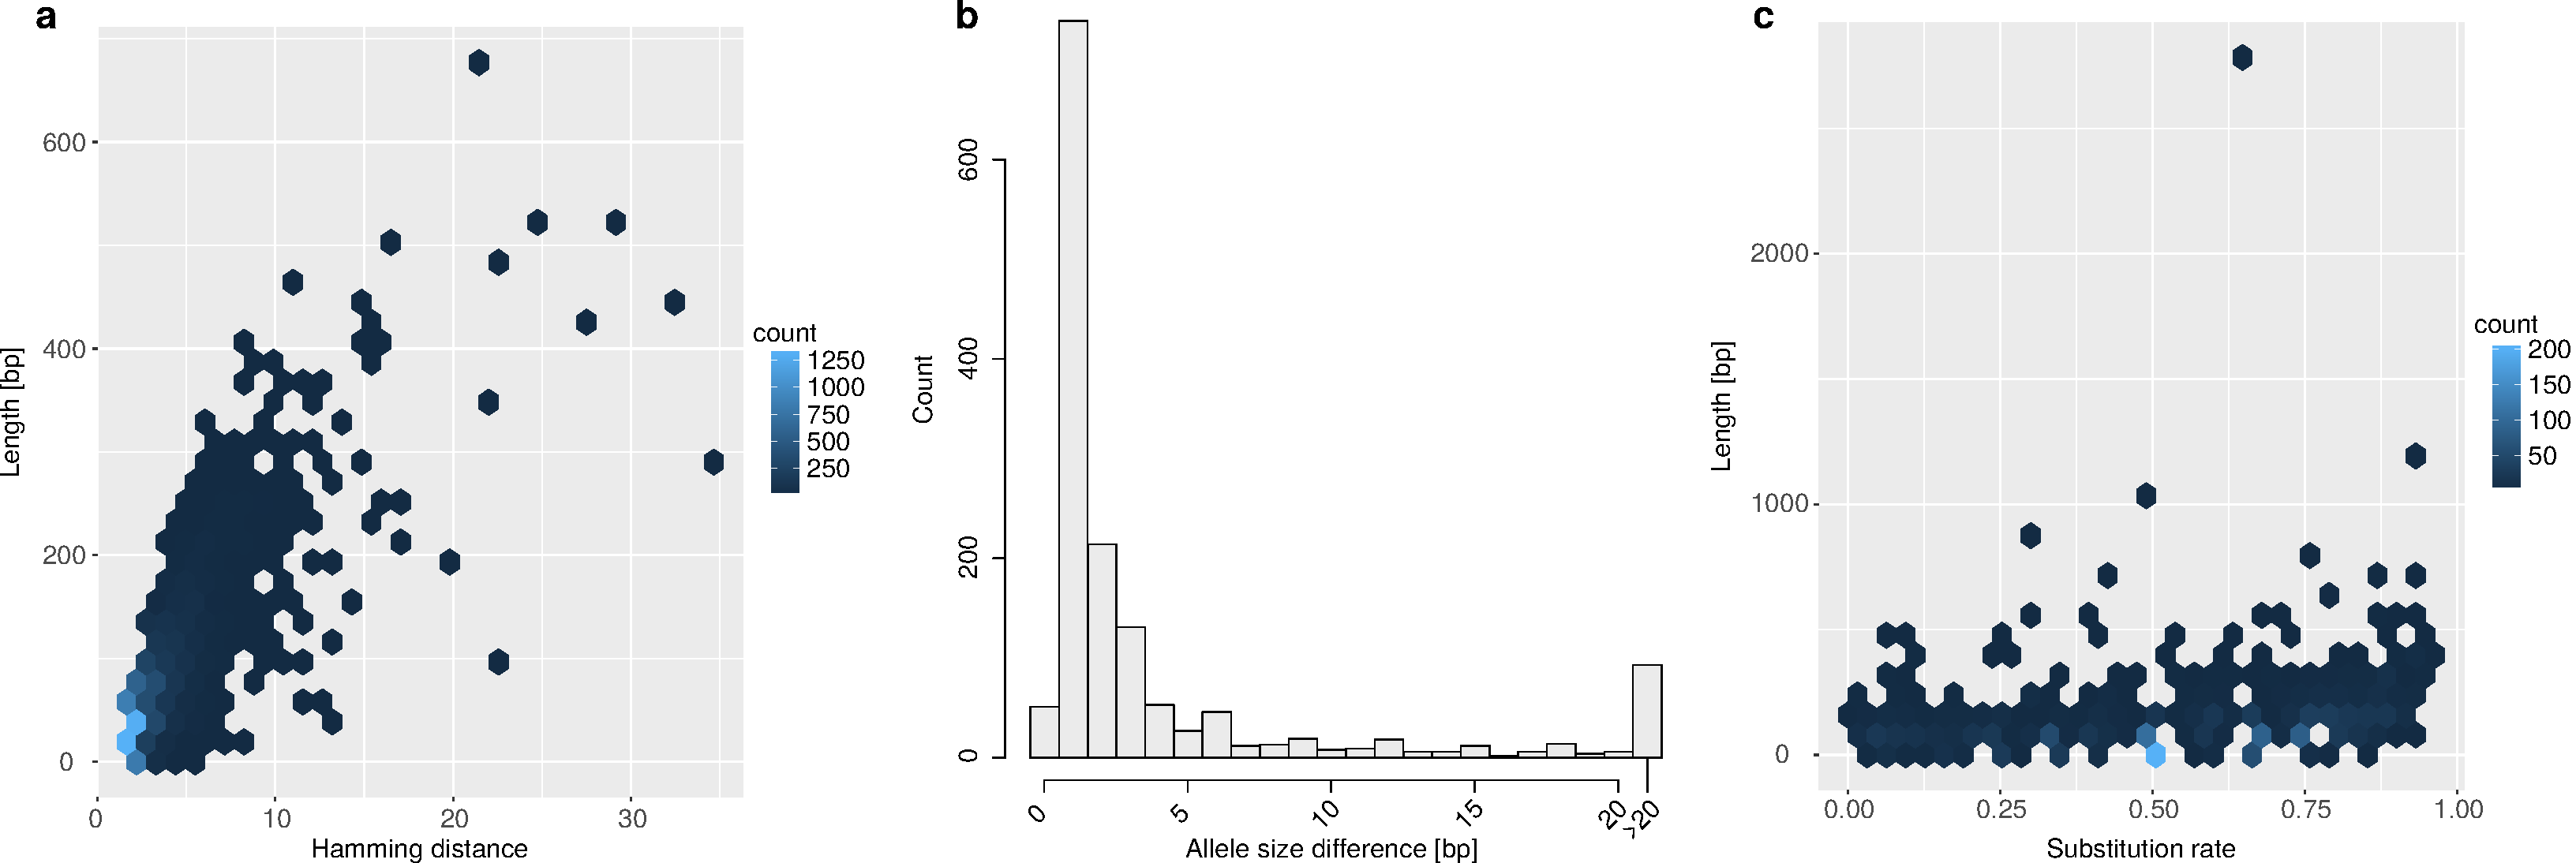
\includegraphics[width=\textwidth]{bubble-breakdown}%
\end{center}
\caption{Structural variation analysis of phased bubbles from our graph-based approach.
a: Joint distribution of allele length and Hamming distance, for pure substitutions.
b. Distribution of size difference between the two alleles, for mixed bubbles and indels. 
Pure substitutions always have a size difference of 0, and are not included in the figure.
c. Joint distribution of the length of the longer allele and the substitution rate, for mixed bubbles.
With a higher substitution rate, the bubble has more substitutions, and with a lower rate more indels.
}
\label{fig:bubble_breakdown}
\end{figure*}

\textit{Bubble characterization}.
We attempted to characterize the nature of the heterozygous genomic variation encoded in the phased bubbles.
There are 25,033 bi-allelic bubbles phased by our approach when using 30$\times$ coverage PacBio data.
Of these bubbles, there are 15,293 for which both allele sequences have a length of at most 1\,bp, out of which 15,258 are single base pair substitutions (SNVs) and 35 are 1\,bp indels.
The remaining 9,740 bubbles either encode two or more small variants or more complex differences.
To differentiate these cases, we computed an alignment between the two allele paths and refer to those bubbles for which the alignment contains only substitutions but no indels as ``pure substitutions''.
Figure~\ref{fig:bubble_breakdown}a shows the joint distribution of length and (Hamming) distance for these pure substitution bubbles.
This analysis reveals, on the one hand, that many longer pure substitions have a low distance and hence encode multiple SNVs and, on the other hand, that there also exists a population of more complex substitutions.
For the 1,489 bubbles not classified as pure substitutions, which we refer to as ``mixed bubbles'', Figure~\ref{fig:bubble_breakdown}b shows the absolute length difference between the two alleles.
While this difference is small for most bubbles, there are 93 bubbles with a length difference of 21\,bp or more.
To further elucidate the nature of the sequence differences, Figure~\ref{fig:bubble_breakdown}c presents the joint distribution of length of the longer allele and substitition rate, which is defined as the fraction of substitutions among all edit operations done to align the two sequences. (That is, a pure insertion or deletion has a substitution rate of 0.)

% the x-axis represents the edit distance between the two allele (haplotype) paths,
% % \todo{I wouldn't call this type and talk of edit distance right away. Confusing otherwise.} 
% and the y-axis represents the maximum length from these two haplotype sequences for each bubble.
% % The structural variant type for each bubble is determined by calculating the edit distance between the two allele (haplotype) paths, and the maximum variant size is calculated by considering the maximum length from these two haplotype sequences.
% The color of each point in the plot indicates the number of corresponding bubbles.
% Using our approach, in Figure~\ref{fig:sv_scatter}, we observe that 17,733 bubbles (out of 29,071) are at a bottom left corner with an edit distance of 1 bp, indicating that the bubbles describe SNVs or 1 bps indels. 
% There are a few points that lie on the diagonal (i.e. with one edit per base in the longest allele), which represent larger indels.
% % \todo{Also below 20bp, right?}.
% The points along the vertical line and those in between vertical and diagonal of the plot represent the bubbles containing SNPs or indels that are close to each other and that end up being contained in a single bubble.
% Furthermore, we see that some points represent larger and more complex variation.
% Overall, the distribution of phased bubbles in the plot indicates that the graph-based approach using both Illumina and PacBio data can phase both small and large structural variants.

% Taken together, the above analysis shows that our graph-based approach delivers better diploid assemblies even at lower PacBio coverages.
% In addition, the graph-based approach helps to detect and phase larger structural variants present in the diploid genomes.

% \begin{figure}[t!]\centering
% \includegraphics[width=\columnwidth]{falcon_bubbles.pdf}
% \caption{Structural variation analysis of phased bubbles from Falcon Unzip. The x axis and y axis show edit distance and maximum size for the two haplotype paths going through each bubble. The color shows the density of bubbles.}
% \label{fig:sv_scatter_falcon}
% \end{figure}

\section{Discussion}
The Falcon Unzip method \citep{chin2016phased} is based purely on PacBio reads, which exhibit a high error rate; it is therefore not suitable for lower coverages.
By using (costly) high coverage PacBio data, Falcon Unzip can generate good quality assemblies with an average haplotig identity of up to 99.99\% \citep{chin2016phased}.
% \todo{I do not see this number in the table above}. %, which is not the cost-effective way to solve the problem.
However, it follows a conservative approach for phasing genomic variants.
As sketched in Figure~\ref{fig:ex_graph_approach}, Falcon Unzip generates long primary contigs, but tends to phase them only partially.

To address the above problems, we have created a novel graph-based approach to diploid genome assembly that combines different sequencing technologies.
By using one technology producing shorter, more accurate reads, and a second technology delivering long reads, we produce accurate, complete and contiguous haplotypes. 
Our method also provides a cost-effective way of generating high quality diploid assemblies.
By performing phasing directly in the space of sequence graphs---without flattening them into contigs in intermediate steps---we can phase large structural variants, which is not possible using linear approaches. 
We have tested our approach using real data, in the form of a pseudo-diploid yeast genome, and we have shown that we deliver accurate and complete haplotigs.
Furthermore, we have shown that we can detect and phase structural variants.

In this study, we restricted ourselves to phasing unique, non-repetitive regions of the genome.
As a next step, we plan to develop techniques for phasing repetitive regions as well.
Resolving repeats and polyploid phasing are closely related problems, as pointed out by \cite{Chaisson2017}.
Therefore, we will aim to solve heterozygous variants and repeats in a joint phasing framework, in order to obtain even more contiguous diploid genome assemblies that include both types of features.
The machinery we plan to develop for this purpose would also remove the need to run an external assembler (Canu) for bubble ordering.
Finally, our framework allows, in principle, for incorporating additional data from other sequencing technologies, such as chromatin conformation capture \citep{burton2013chromosome}, linked read sequencing \citep{weisenfeld2017direct}, and single-cell template strand sequencing (Strand-seq; \citealp{Porubsky2016}).
In previous studies on reference-based haplotyping, we have shown such integrative approaches to be very powerful when infering chromosome-scale haplotypes \citep{porubsky2017dense,chaisson2017multi}; we believe similar results can be obtained for \textit{de novo} diploid genome assemblies.
Moreover, studying the biological implications of the phased structural variation we can now detect also constitute an exciting future research direction.


  \chapter{Conclusions}


%%% Local Variables:
%%% mode: latex
%%% TeX-master: "main"
%%% End:

 {
%\bibliographystyle{unsrtnat}
   \bibliographystyle{apalike}
   \bibliography{main}
 }
\appendix
\appendixpage
\noappendicestocpagenum
\addappheadtotoc

\chapter{Additional Details}

\section{Proof of Lemma~\ref{lem:SWC}}\label{app:SWC}
\begin{proof}
    We show the claim by using a randomized argument. 
    To this end, we assume that for each $i$, the rows from $R_i$ and $S_i$ are selected uniformly at random from $R_i \cap \tau(M)$ and $S_i \cap \tau(M)$ and
    the rows from $R'_i$ and $S'_i$ are selected uniformly at random from $R'_i \cap \tau'(M)$ and $S'_i \cap \tau'(M)$.
    We argue that for each column, the expected number of errors is at most a factor $(1 + O(\epsilon))$ larger than in an optimal solution.
    Then the claim follows from linearity of expectation and the fact that there is a selection with at most the expected number of errors. 

    We consider the $j$th column of $M$.
    Let $c := \tau(M)_{*,j}$, but without rows that have an entry ``$-$'' in column $j$.
    Let $p := |\{ i : c_i = 0\}|/|c|$ be the fraction of zeros in $c$.
    By swapping the zeros and ones we can assume \WLOG that $p \ge 1-p$, \ie, $p \ge 1/2$.
    Our assumption implies $\tau_j = 0$ and the optimal solution has $(1-p)|c|$ errors within $c$.

    The general idea of the proof is as follows.
    Suppose we would select exactly one row from $\tau(M)$ uniformly at random.
    Then with probability $p$, the algorithm has $(1-p)|c|$ errors in $c$ and with probability $(1-p)$ the number of errors is $p|c|$.
    Therefore the expected number of errors is $(p(1-p) + (1-p)p) |c| = 2 p (1-p) |c|$.
    We obtain the approximation ratio $2 p (1-p) |c| / ((1-p)|c|) = 2 p$.

    We will see that the approximation ratio improves with choosing several rows instead of a single one.
    Additionally, we have to handle the circumstance that we only sample from $U \cup L$ and ignore $X$.

    There is a further issue regarding $U$.
    Let $s$ be the smallest index such that $R_s$ and $c$ intersect, \ie, $R_s$ is the first set with binary entries in column $j$.
    Then rows sampled for $R_s$ may be located outside of $c$ at positions with wildcards in column $j$.
    We avoid the complications caused by the wildcards by only considering classes $R_{i}$ for $i > s$.

    To summarize, $c$ has at least $\epsilon r$ selected entries and we ignore at most $2 \epsilon^2 r$ of these due to $X$ and $R_s$.
    For each $i > s$, we sample $1/\epsilon^3$ rows from $R_i$. 
    Let $c'$ be $c$ restricted to $\bigcup_{i > s} R_{i}$ and let $c''$ be $c$ restricted to  $L$.
    Let $\hat{c}$ be $c$ without $R_s$ and $X$ and let $\bar{c}$ be the part of $c$ in $X \cup R_s$.
    For each $i$, let $c'_i$ be the fraction of zeros of $c'$ in $R_i$ and $c''_i$ the fraction of zeros of $c''$ in $S_i$.

    For each $i \le \ell$, we define $p'_i$ to be the fraction of zeros $c'_i$ and $p''_i$ the fraction of zeros $c''_i$.

    We define a random variables $Y'_{i,k}$ for each $s < i \le 1/\epsilon^2$ and $Y''_{i,k}$ for each $1 \le i \le 1/\epsilon^2$. 
    In both cases, $1 \le k \le 1/\epsilon^3$.
    For each $i,k$, we pick an entry from $c'_{i}$ ($c''_i$) uniformly at random. 
    Then $Y'_{i,k}$ ($Y''_{i,k}$) is the value of the picked entry.
    For all $i,k$, $E[Y'_{i,k}] = 1 - p'_{i}$ and $E[Y''_{i,k}] = 1 - p''_i$. 
    Observe that the $Y_{i,k}$ are independent Poisson trials.
    Let $Y' := \sum_{s<i ,1 \le k \le 1/\epsilon^3} Y'_{i,k}$ 
    and $Y'':= \sum_{i, 1 \le k \le 1/\epsilon^3} Y''_{i,k}$.
    We want to use Chernoff bounds to control the probability to take the wrong decision.
    It is sufficient to consider $Y'$ with $s = 1/\epsilon^2-1$, since in all other cases the probabilities are amplified more.
    Let $\mu' := E[Y']$.
    We analyze the ranges of $\mu'$ separately.
    \subparagraph{Case 1:} Let us assume that $\mu' \in [0,1/(2\euler\epsilon^3)]$.
    We define $\delta' := 1/(2\mu'\epsilon^3) - 1$.
    Using a multiplicative Chernoff bound (cf.~\cite{MU05_probability}), we obtain
    \begin{align}
        \Pr(Y' \ge 1/(2\epsilon^3)) &< \Bigl(\frac{\euler^{\delta'}}{(1+\delta')^{(1+\delta')}}\Bigr)^{\mu'} = \Bigl(\frac{1}{1 + \delta'}\Bigr)^{\mu'} \Bigl(\frac{\euler}{{1 + \delta'}}\Bigr)^{\mu'\delta'}\\
        &= (2 \mu' \epsilon^3)^{\mu'}(\euler \cdot 2\mu'\epsilon^3)^{(1/(2\epsilon^3)  - \mu')}\label{eq:rhs}
    \end{align}
    Note that both terms of \eqref{eq:rhs} are numbers between zero and one.
    If $\mu' < 1/\epsilon$, the right term is smaller than $\epsilon^4 \mu'$. 
    Otherwise the left term is smaller than $\epsilon^4 \mu'$

    The range of $\mu'$ implies that the majority of entries in $\hat{c}'$ is zero.
    Recall that $\hat{c}'$ has an $\epsilon^3 \mu'$ fraction of zeros.
    The expected number of errors done by the algorithm is therefore at most
    $(1 - \epsilon^4 \cdot \mu') \cdot (\epsilon^3 \mu') + \epsilon^4 \cdot \mu' \cdot (1 - \epsilon^3 \mu') = (1+\epsilon) \epsilon^3 \mu'$.

    \subparagraph{Case 2:} Let us assume that $\mu' \in (1/(2\euler\epsilon^3), 1/(2\epsilon^3) - 1/\epsilon^2]$.
    We use Hoeffding's inequality \cite{Hoe63_probability} to analyze the range.
    To this end, we scale $Y'$ and obtain $\bar{Y}':= \epsilon^3 Y'$, which has values between zero and one.
    Then 
    \[
        \Pr(\bar{Y}' - E[\bar{Y}'] \ge \epsilon) \le \euler^{-2\epsilon^2/\epsilon^3} = \euler^{-2/\epsilon}\,.
    \]

    Since for sufficiently small $\epsilon$, $\euler^{-2/\epsilon} < \epsilon/(2\euler) \le \epsilon^4 \mu'$,
    again we obtain a $(1+\epsilon)$-approximation in expectation.

    All other ranges now follow immediately:
    For $\mu' \in (1/(2\epsilon^3) - 1/\epsilon^2,1/(2\epsilon^3)]$ every solution is a $(1+O(\epsilon))$-approximation and for larger $\mu'$ the majority of entries in $\hat{c}'$ is one.
    The analysis is analogous.

    In order to combine $Y'$ and $Y''$, we introduce a bias for $Y'$ such that we count rows $i$ for $s < i \le \ell$ with a factor $(1-\epsilon)/(\epsilon - \epsilon^2)$.
    Then
    \[
        \bar{Y} := \frac{\bar{Y}' \cdot (\ell-s)(1-\epsilon)/(\epsilon - \epsilon^2) + \bar{Y}'' \cdot \ell}{(\ell-s)(1-\epsilon)/(\epsilon - \epsilon^2) + \ell}\,.
    \]
    Then, using the union bound, setting $\sigma_j = 0$ for $\bar{Y} < 1/2$ and $\sigma_j = 1$ otherwise gives an expected $1+O(\epsilon)$ approximation within $\hat{c}$.
    Errors in $\bar{c}$ are either also errors in an optimal solution, or they contribute at most a factor $O(\epsilon)$ to the total number of errors.
    Thus overall we obtain an approximation ratio $1+O(\epsilon)$ within $c$.
    The algorithm $\SWC$ has at most the same approximation ratio, since the only difference is that we do not fix the $Y_{i,k}$ to be zero or one.
    Thus the random process used by the algorithm can only have a lower variance.

    This finishes our analysis for $\tau(M)_{*,j}$.
    For $\tau'(M)_{*,j}$, the proof is analogous.

    % I DON'T UNDERSTAND THE FOLLOWING ANYMORE, THEREFORE COMMENTED.
    %To finish the proof we still have to argue that we may assign the $r$ rows with maximal values $d_i$ to $\sigma$ and the remaining $r'$ rows to $\sigma'$.
    %The reason is that at all times we compare against the assignment of $(\tau,\tau')$, which is a stronger result then the mere approximation ratio.
    %Since $|\tau(M)|=r$ and the choice of $d_i$ gives the assignment with fewest errors, the claim follows.
\end{proof}

We introduced a small but easy to handle imprecision due to the assumption that we can choose exactly the same number of strings from each range.



%%% Local Variables:
%%% mode: latex
%%% TeX-master: "main"
%%% End:

\listoffigures
\listoftables
\listofalgorithms
\end{document}
